\documentclass{article}

% Language setting
% Replace `english' with e.g. `spanish' to change the document language
\usepackage[english]{babel}
\usepackage{natbib}

\usepackage{algorithm}

\usepackage{caption}
\usepackage{array}% For line breaks in cells
\usepackage{subcaption}

\usepackage{algorithmic}

\usepackage{tikz}
\usepackage{float}
\usetikzlibrary{trees}
\usetikzlibrary{mindmap,trees}
\usetikzlibrary{arrows.meta, positioning, shapes.geometric, fit, backgrounds}


% Set page size and margins
% Replace `letterpaper' with `a4paper' for UK/EU standard size

\usepackage[letterpaper,top=2cm,bottom=2cm,left=3cm,right=3cm,marginparwidth=1.75cm]{geometry}

% Useful packages
\usepackage{amsmath}
\usepackage{amsfonts}
\usepackage{graphicx}
\usepackage[colorlinks=true, allcolors=blue]{hyperref}

\renewcommand{\arraystretch}{1.4} % More vertical space
\setlength{\tabcolsep}{6pt} % More horizontal padding

\title{Enabling Sample Efficient Design Space Exploration through Machine Learning}
\author{Joshua Hellewell}

\begin{document}

\maketitle

\newpage{}

\begin{abstract}
In engineering, design problems are often complex with components composed of intricate parts and features that define the functionality or performance of the component. One of the key driving activities to enable engineering innovation is design exploration and optimisation, referring to the ways in which potential designs are identified that result in the most optimal performance being realised in context of an objective. To determine this, and as is common in industry, numerical tools such as Computational Fluid Dynamics (CFD) or Finite Element Analysis (FEA) are used to provide performance data associated with engineering designs (e.g., lift performance for an aerofoil or heat losses for a heat exchanger). These tools are computationally expensive and not suited to fast, iterative design exploration, attributed to the computational cost of solving physical equations to provide numerical data. They are typically used towards the end of a design process, downstream of opportune points to iterate or change designs. This computational burden generally increases with added complexity in the inputs, such as number of elements in unstructured meshes, point clouds or voxels.

In contrast, optimisation methods rely on our ability to parameterise the problem in an efficient way. While simpler shapes such as tubes or rings can be easily parametrised by properties such as radius or thickness to enable a well-defined set of search dimensions that correspond to different design configurations, more complex shapes such as turbo-machinery components, or intricate heat exchange surfaces cannot be concisely described by a finite set of parameters and reside in high-dimensional geometry representations. As part of this research, supported by a comprehensive literature review, we will investigate approaches to representing high-dimensional engineering problems in a low-dimensional space to overcome the \textit{curse of dimensionality}, therefore enabling efficient design space exploration and optimisation. Identified methods will be implemented to develop a framework for embedding such representations into a proof-of-principle geometric optimisation problem. One of the key research objective will be to investigate and asses the interpretability and controllability of the low-dimensional representations to enable targeted design modification and optimisation in this intermediate low latent space manifold.
\end{abstract}

\noindent \textbf{Keywords:} Design optimisation, Machine learning, Dimensionality reduction, Variational autoencoders, Generative adversarial networks
\newpage

\tableofcontents  % <-- This generates the Table of Contents
\newpage          % Optional: start next content on a new page

\section{Introduction}

Engineering innovation is an iterative process that often involves exploration of vast design spaces under specific constraints to identify configurations that result in optimal solutions according to performance objectives \cite{Yamada2022}. These objectives, for example, could include minimizing aerodynamic performance metrics such as drag or minimizing material usage in manufacturing processes through optimal geometry configurations. Approaches for evaluating the objective function may include measurements on a prototype implementation, complex numerical simulation or estimates based on analytical models \citep{Pimentel2022}. Complex computational tools such as finite element analysis (FEA) and computational fluid dynamics (CFD) \citep{Archbold2024} are often used as part of optimisation frameworks as substitutes for physical prototyping and testing of solutions. 

While such tools are often noted as being cost-effective alternatives to physical implementations of designs, numerical tools themselves are known to be computationally expensive taking a long time to execute \citep{Shi2010}. They are not well suited to multi-query problems such as optimisation, uncertainty quantification, and inverse problems \citep{Archbold2024}. Optimisation problems that depend on computationally expensive fitness evaluations are termed Expensive Optimisation Problems (EOPs)\citep{Ren2025}. As a result, numerical tools are rarely used to assess performance for every design iteration; rather, they are used as a performance verification before committing to final designs. Solving such design problems becomes even more challenging when the input space is high-dimensional, as well as being computationally expensive to evaluate \citep{Tripp2020}, particularly if used with inefficient design exploration approaches such as grid-search, which would require simulations to be run for every conceivable configuration of design parameters. 

For example, if we define a design space by only two parameters, and each parameter has 50 potential values, there would be 2500 design configurations—each of which would require assessment via costly numerical simulations. Extending this to three design parameters reveals $1.25 \times 10^6$
configurations, which soon becomes computationally intractable in any reasonable time frame if dependent on costly function evaluations (FE). Further, it would be naïve to assume that two or three design parameters would effectively describe the features that define real-world components. Such a problem is known as the \textit{curse of dimensionality} \citep{Keogh2017}, whereby the number of FEs grows exponentially with the number of search dimensions. Typical components in industries such as aerospace may be composed of vastly unique features and complex sub-features that cannot be easily, if at all, parameterized by standard methods. For 2D aero-foils, tens of design variables are common, whereas for 3D wing problems, hundreds or thousands of shape design variables may be necessary \citep{Jabn2024}. In these cases, the design space becomes a function of the data representation itself, where common intermediate representations of 3D shapes include unstructured meshes, point clouds, and voxel representations \citep{Jabn2024}. In the context of design optimisation and other multi-query applications, it is necessary to limit the input dimensions for computational tractability \citep{Jabn2024}. However, real-world engineering designs are typically composed of multi-million element unstructured meshes, and in the absence of a set of concise descriptors, the design space becomes infeasibly complex, with each mesh cell, voxel, or point cloud having the freedom to occupy all values in space for all configurations. 

To highlight this, assuming a 3D voxel grid of dimensions \( 128\times128\times128 \), and an arbitrary 3D shape \( S \) contained within, defined by 100 nodes, the total design space would include every combination of \( x,y,z \) position for each of the 100 nodes. That is:
\[
2^{128\times128\times128} =  2^{2097152}
\]
configurations. This is more than the number of atoms in the universe. Consequently, the search space has many constraints and only a small feasible region \citep{Shi2010} increasing the risk of missing global optimum solutions.

For this reason, one of the biggest challenges in engineering design optimisation is finding ways to effectively parameterize designs such that we can numerically and concisely (using a low number of variables) describe how one arbitrarily complex shape relates to another, thus reducing the dimensions of the design space and enabling more efficient sampling. In doing so, optimisation methods including non-gradient-based \citep{Hare2013} (e.g., evolutionary algorithms and Bayesian optimisation) and gradient-based methods can be employed to find solutions to real-world optimisation problems. See \citep{Roy2008} for a review of some historicaly popular optimisation approaches.

 Conventional approaches to parameterizing engineering components include B-splines, Bezier curves, and free-form deformation \citep{Jabn2024}, however, such methods are limited and are not suited to the most complex of components. As part of this research, machine learning will be explored as a means to enable transformation of a high-dimensional problem into a low-dimensional, sample-efficient form, commonly regarded as the \textit{latent space}. 

Machine learning, a subfield of artificial intelligence, has emerged as a dynamic approach for dimensionality reduction that enables data compression, which can work on complex datasets and is not constrained to the linear bounds of conventional dimensionality reduction techniques such as Principal Component Analysis (PCA) \citep{Lew2021} or Singular Value Decomposition. However, in reality, problems require non-linear approaches \citep{Jabn2024}. Popular among the literature to address these limitations are variational autoencoders (VAEs) and generative adversarial networks (GANs). These models belong to a category of machine learning known as \textit{unsupervised generative models}, whereby they learn from the data a mapping from input data to a reconstruction of itself \citep{Lew2021}. 

These methods provide a reduced-dimension representation of a data distribution in the form of a continuous latent space, which is a concise descriptor of the underlying data distribution itself \citep{Zheng2023}, represented as set of latent variables \citep{Jabn2024}. Depending on the complexity of the underlying data distribution, the dimension of this latent representation will vary, and it is necessary to find an optimal representation dimension that balances \citep{Lew2021}: 

\begin{enumerate}
    \item A useful degree of dimensionality reduction.
    \item Maintaining an effective reconstruction of the original data.
\end{enumerate}

The former supports sample-efficient design space exploration, while the latter ensures that the reconstruction from the latent representation results in realistic, representative data samples. More generally, the bottleneck layer, or the latent representation, should preserve meaningful information about the original data while reducing its complexity and dimensionality \citep{Zheng2023}. Simply enabling an exact reconstruction of the data yields limited benefit; this would simply be an identity function. 

The mentioned methods are embedded with continuity constraints that enable interpolation through the low-dimensional manifold, which gives the opportunity to leverage gradient-based optimisation methods or simply discover novel data that matches the original data distribution. Commonly seen in VAEs is the Kullback-Leibler (KL) divergence, which acts to penalise any divergence from the original data distribution \citep{Zheng2023}, therefore enforcing a physical similarity between deconstructed, adjacent samples in the low-dimensional space.

Unique to this research will be the abstraction of the methods to a simplified optimisation problem to avoid distraction from the underlying concepts. In contrast, in the literature, such methods are often coupled with complex problem applications. Attempting to demonstrate and validate a method when deployed to an overly complex domain problem will likely result in limited insight into the predictive capability itself. Therefore, it is necessary to validate at varying levels of complexity to build up understanding and identify limitations free from problem-specific domain complexities \citep{Hobbs2021}. 

This research focuses on a simplified problem statement to investigate and assess methodologies for interpretability and controllability of low-dimensional representations, enabling targeted design modification and optimisation.

\newpage

\section{Problem Statement and Background}

\subsection{Geometric Representation}\label{Geometry}

Despite the widespread application of 3D geometries in various industries, the underlying concepts to be investigated in this research are applicable to the computationally simpler case of 2D geometry optimisation problems.  While there are a multitude of complex optimisation problems in engineering that could be explored, such as material specific structural properties, or aerodynamic efficiency metrics, their evaluation requires significant upfront computational investment via numerical solvers to determine performance. We opt for a simpler, analytically tractable optimisation problem as a proxy for a computationally expensive numerical simulation, thus avoiding being engrossed in computational inefficiencies and domain-specific expert knowledge requirements.

We consider the case of 2D geometric shapes, defined by a series of connected nodes.
Let the 2D shape be defined by a series of \(N\) nodes, where each node \(P_i = (x_i, y_i)\), with \(x_i, y_i \in \mathbb{R}\) representing the coordinates of the \(i\)-th node. Then, the shape can be expressed as the set:

\[
S_{2D} = \{ P_i \mid P_i = (x_i, y_i), \, x_i, y_i \in \mathbb{R}, \, i = 1, 2, \dots, N \}
\]
where \(N\) represents the number of nodes.

For completeness, though not within the scope of this research, a 3D shape \(S_{3D}\) is defined by a set of \(N_V\) vertices, each represented by coordinates \((x_i, y_i, z_i)\):

\[
S_{3D} = \{ V_i \mid V_i = (x_i, y_i, z_i), \, x_i, y_i, z_i \in \mathbb{R}, \, i = 1, 2, \dots, N_V \}
\]
where \(N_V\) represents the number of vertices in the mesh.

For the 2D geometric optimisation problem under consideration in this research, a fixed connectivity between nodes will be maintained, thereby preventing the defining perimeter of the 2D shapes from varying as a result of node re-connectivity. Any shape change will be achieved through a translation of the individual nodes in the $x,y$ plane. Example shapes with resolution of $N=200$ are shown in in Figure~\ref{fig:randomshapes}. As part of this research, approaches to describing shapes such as those shown in \ref{fig:randomshapes}.


\begin{figure}[htp]
    \centering
    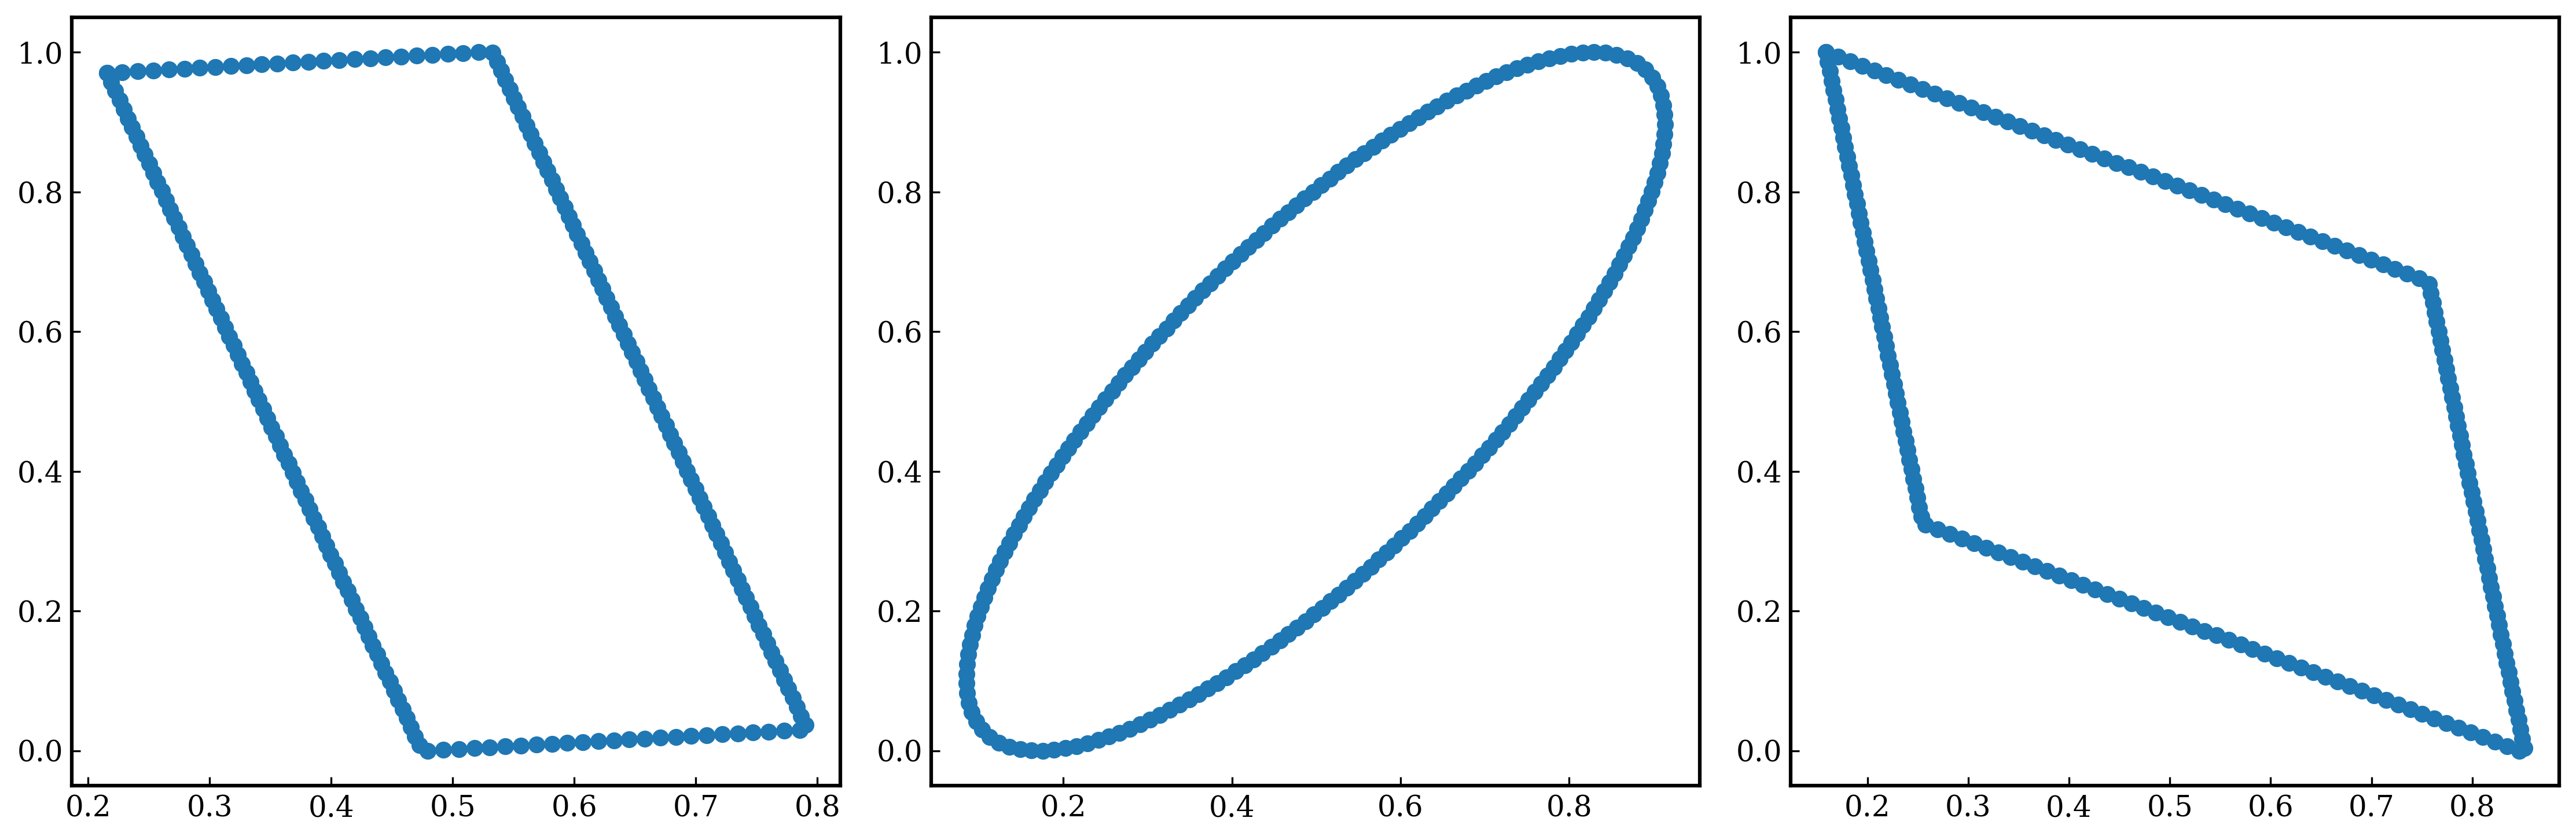
\includegraphics[width=12cm]{figures/output.png}
    \caption{Random shapes, $N=200$}
    \label{fig:randomshapes}
\end{figure}


\subsection{Geometric Optimisation Problem}

The optimisation problem that will be explored in this research will be denoted as 'compactness'. We will use a definition of compactness as outlined in \citep{Bribiesca2008}, denoted as the ratio of the perimeter squared to the area of the 2D as shown in Equation~\eqref{eq:compactness}. This problem has a computationally tractable solution, but will serve as a proxy for complex, expensive simulations in this research. 

\begin{equation}
    \text{Compactness}=\frac{\text{Perimeter}^2}{\text{Area}}
    \label{eq:compactness}
\end{equation}

In the absence of a concise and finite set of of descriptors for the 2D shapes, the design space contains all combinations of configurations for every $x,y$ position of each node $P_i$, defining a shape $S_{2D}$ and therefore \eqref{eq:compactness} would need to be computed for every conceivable configuration of $S_{2D}$ to identify an optimal solution.

Let us consider the case where the potential values for $x_i,y_i$ of each node $P_i$ is constrained to discrete values between 0 and 1 in increments of 0.1. For both $x_i$ and $y_i$, there are 10 potential design values resulting in a total number of potential configurations for each $P_i$ of 100. If $N=100$, such that there are 100 nodes defining the 2D shape, the total design space contains $100^{100}$ potential configurations. This is a significantly large design space. Each of the 100 nodes can be considered a dimension in this problem, and we can demonstrate how adding additional nodes increases the search space exponential, known as the curse of dimensionality \citep{Keogh2017}. Similarly, with 200 nodes, the total number of shape configurations increases to $100^2$.

To evaluate \eqref{eq:perimeter_area}, we must have a method of determining the perimeter and area for any arbitary shape defined by $S_{2D}$. For shapes such as circles there are existing parameterisations and equations that can be used to compute their geometric properties (see Equations~\eqref{eq:areacircle} and \eqref{eq:perimetercircle})

However, for arbitary polygons this is not always the case. 
\begin{equation}
    \text{Area of Circle}= \pi r^2 
    \label{eq:areacircle}
\end{equation}
\begin{equation}
    \text{Perimeter of Circle}= 2\pi r
    \label{eq:perimetercircle}
\end{equation}

To determine the area of any 2D shape $S_{2D}$ defined by nodes $P_i$ we employ the shoelace theorem, also known as Gauss's area formula. This is mathematical method used to find the area of a simple polygon when its vertices are given in order. The theorem works by summing up products of coordinates in a specific way, resembling the crossing of laces in a shoe \citep{Braden1986}.
The Shoelace Theorem states that the area of a simple polygon, $S_{2D}$ with vertices $P_i =(x_1, y_1), (x_2, y_2), \dots, (x_N, y_N)$ arranged in order can be computed as:

\begin{equation}
A = \frac{1}{2} \left| \sum_{i=1}^{n} (x_i y_{i+1} - x_{i+1} y_i) \right|
\label{area_equaton}
\end{equation}
where \((x_{n+1}, y_{n+1}) = (x_1, y_1)\) to close the polygon.

Similarly, the perimeter of the polygon can be determined by summing the euclidean distance between adjacent nodes of fixed connectivity. The perimeter \( L \) of a simple polygon with \( N \) ordered vertices \( P_i = (x_i, y_i) \) can be computed as:


\begin{equation}
    L = \sum_{i=1}^{N-1} d_i + d_N
    \label{perimiter_equaton}
\end{equation}

where \( d_i \) represents the Euclidean distance between consecutive nodes1:
\[
d_i = \sqrt{(x_{i+1} - x_i)^2 + (y_{i+1} - y_i)^2}, \quad \text{for } i = 1, \dots, N-1
\]
The final segment that closes the polygon is:

\[
d_N = \sqrt{(x_1 - x_N)^2 + (y_1 - y_N)^2}
\]

\subsection{Design Space Exploration}
Design space exploration (DSE) is the process of realing a design solution or solutions that best satisfy the design requirements from a space of tentative design points \citep{CARDOSO2017255}. For the geometry representation described in \ref{Geometry}, the total design space for all 2D shapes is vast, and due to the continuous freedom that the $x_i,y_i$ coordinates can occupy, the total design space is infinitely complex, including every combination of every node in all positions in $x_i,y_i$. Introducing freedom for the connectivity between nodes to change would also add additional complexity to the search space. In reality, constraints are applied to the design spaces to enforce logical and appropriate design outcomes. Such constraints may come from prior knowledge of a particular domain, or may be prescribed by manufacturing capabilities (e.g., design must fit on the print bed of a 3D printer). Further, the associated performance surface, that is the evaluation of the performance objective (See equation~\eqref{eq:compactness}) is non-linear and non-convex meaning there are often multiple local optima. 

Ineffective searches may result in designs being selected at local optima, and not global optima. Often in real-world design engineering, there are often multiple design objectives to optimise for which adds additional complexity the the already non-linear performance spaces - this is known as multi-objective (DSE) \citep{Pimentel2022}.  Examples of this performance surface will be explored in the results section. The combination of a large design space, and non-convex performance surface means identifying optimal designs is not trivial and necessitates the user to utilise an appropriate design space search strategy, or alleviate the aforementioned challenges. In engineering, the costly nature of design, and subsequent redesign mandates that design space exploration with the aim of identifying optimal soltutions should be performed as early as possible, as this will often contribute to the success or failure of the final product \citep{Pimentel2022}.

Some search search strategies rely on heuristics to prune the search space, that is using expert knowledge or intuition to explore designs in regions regarded as appropriate to the designer or known to be performant based on prior knowledge \citep{Nardi2018}, however this is typically unfeasible due to the complexity of the search space and noise within as a method of comprehensively searching for new designs \citep{Zheng2023}. This approach also puts significant reliance on the designers, and will often limit the discovery of new optimal designs to the tendency to explore known configurations. This approach will often be complimented by random searches, or brute force methods \citep{Huang2022}. In all cases, regardless of the design search strategy employed should provide a reasonable balance between confidence, convergence to an optima and required effort \citep{Pimentel2022}.

Search strategies can be split into \textit{exact} and \textit{non-exact} method, whereby exact methods guarantee the realisation of an optimum solutions. In contrast, non-exact methods utilise \textit{metaheuristics}, providing a design solution that satisfied the performance objective as best as possible. The former is often compute intensive, requiring pruning techniques to optimise for efficiency in vast design spaces though in reality do not scale well for real-world, complex applications. Metaheuristic approaches include hill-climbing, tabu search, simulated annealing, ant colony optimisation, particle swarm optimisation, and genetic algorithms \citep{Panerati2016}. In this section, we will explore some of the popular search strategies and their usage in engineering design optimisation workflows.

\subsubsection{Genetic Algorithm (GA)}\label{GA}
The genetic algorithm is a type of evolutionary algorithm referring to strategies that discriminate and down select optimal solutions according a specified performance metric. They are widely used in design space optimisation, as they do not require any prior knowledge to implement, navigating to solution by the principle of starting from random population of solutions, and iteratively improving upon those \citep{Panerati2016}. Evoltuionary methods such as GA are not guaranteed to find an optimal solution, however generally find good enough solutions if permitted to search and explore for sufficiently large numbers of evolutions. The pseudo code for this can be seen in Algorithm~\ref{alg:GA} \citep{Sivanandam2008}.

\begin{algorithm}
\caption{Genetic Algorithm}
\begin{algorithmic}[1]
\label{alg:GA}
\STATE \textbf{Initialize} population with random individuals
\WHILE{stopping criteria not met}
    \STATE \textbf{Evaluate} fitness of each individual in the population
    \STATE \textbf{Select} parents based on fitness
    \STATE \textbf{Apply Crossover} to create offspring
    \STATE \textbf{Apply Mutation} to offspring with some probability
    \STATE \textbf{Form new population} by selecting individuals from parents and offspring
\ENDWHILE
\STATE \textbf{Return} best solution found
\end{algorithmic}
\end{algorithm}

One of the most popular approaches to the genetic algorithm is the Non-dominated Sorting Genetic Algorithm (NSGA) often used for multi-objective optimisation problems. This approach differs from the classicial method in that it develops a set of fronts, based on dominance by solutions found in the initialised populations. Crossover and mutations operations are the same as that described in Algorithm~\ref{alg:GA}, however, prior to selection, the population is assigned a scored based on the individuals non-dominance. This results in two measures for the scoring of fitness. Firstly, a non-dominated rank using the Pareto front dominance, and secondly a crowding distance score to encourage divesity of the population assigning high scores to individuals who score high but are distanced from neighbours \citep{SrinivasN1994}.

In applying the genetic algorithm to design space exploration and optimisation, it is necessary to represent your engineering design problem in a format compatible with GA, meaning defining a suitable parameterisaton of the design space. For GA, each individual design represents a biological individual where the complete collection of all shapes/designs is referred to as $X$. This population $X$ includes each $X_i$ individuals from each generation and is composed genes $x^n_{i,j}$. In the context of the geometric shape optimisation problem described in \ref{Geometry}, the genes would be each of the individual node points, $P_i$. The initial random population of individuals would be some finite number of shapes $S_{2D}$. Each individual $X_i$ has a fitness function, that is a the measure of the performance, like that shown in Equation~\eqref{eq:compactness} - though more generally we will refer to this as fitness measure, $FM(X_i)$. In many engineering applications, this fitness measure may be determined via experimentation, or numerical simulation \citep{Pimentel2022}. As a result, this encourages efficiency and accuracy in the selection of individuals in which to perform evaluations, attributed to the numerical or physical cost associated of assessing individual suitability. However, our abstracted geometry optimisation enables rapid, and direct fitness evaluation via computation of \eqref{eq:compactness}.

\cite{Kim2021} use a genetic algorithm to explore potential design solutions for 11x11 grid composites, using the GA to propose potentially improved candidate, determined via finite element analysis (FEA) while also combining domain knowledge via constraining the explored solutions according to some prescribed domain conditions. This results in a an acceleration of the optimisation process compared to conventional GA. \cite{Taj2023} employs GA in a multi-objective optimisation problem coupled with CFD for optimising for drag, and low radar cross section (RCS) -  a pair of conflicting requirements in aerodynamic design. They are able to achieve a  6.7\% reduction in drag and 50.9\% in RCS. Their framework also incorporates a surrogate model in place of the costly numerical simulation in the form of Gaussian Processes to enable a speed up of the performance evaluation step thus enabling more generations to be explored.

While GA is effective in moving towards an optimal solution, it still requires the evaluation of fitness measure by means of numerical simulation, or analysis or some surrogate approach. In \cite{Taj2023}, 20401 function evaluations were performed to find the optimal geometry, made computationally  tractable by the use of an efficient GP-based surrogate model. In it's absence  such numerous evaluations would be computationally infeasible. The analytically tractable nature of the geometric optimisation problem in this study circumvents this, enabling rapid evaluation of the fitness measure. In general, the larger the number of dimensions in the design space (genes), the larger the initial population and the more generations are required to reach a viable solution by enabling more \textit{exploratory} steps, across a more comprehensive set of initial design points \citep{Gibbs2011}. This is a result of a large number of design dimensions increasing the search space exponentially \citep{Keogh2017}, and therefore the larger initial population gives better coverage of this space, reducing the risk of premature convergence. For this reason, seeking to reduce this dimensional complexity while retaining critical information enables more efficient utilisation of optimisation methodologies and mitigates against the \textit{curse of dimensionality} \citep{Serani2024}. Alternatively, rather than trying to reduce the number of dimensions in the search space, it is common, often in early design stages to reduce the volume of the design space according to constraints put on defining varaibles according to prior domain knowledge.


\subsubsection{Gradient-based Design Exploration}
While heuristic based search strategies are common, and often result in sufficiently good enough solutions with respect to the global performance optima, in some critical applications, finding guaranteed optima is necessary. With evolutionary strategies, there is a risk that many potentially viable solutions are missed unless the approach is compensated for by running the evolutionary algorithms multiple times, with varying starting conditions (e.g., algorithm settings, objective priorities). Though in reality, this is not ideal and using a more robust, guaranteed approach is preferred. Additionally, while gradient-free methods (such as GA) tend to have quadratic or cubic growth factors for evaluations with respect to increases in design variable dimensions, gradient-based methods follow a more linear trend \citep{Li2022}. \cite{Li2022} also highlight that gradient-based optimisation approaches are the most suitable to overcome the conflicting challenges of high-computational cost of typical evaluation simulations, and the high-dimensionality of the geometric design space often encountered with complex engineering design applications, attributed to their ability to efficiently search high-dimensional spaces.
In contrast, the sub category of optimisation methods built upon the principle of calculating or estimating the gradient of the objective function are known as gradient-based methods. With such approaches, the gradient provides information on how the objective function is changing with respect to the design variables \citep{Brown:2018:2518-6582:1}. Updates to the design variables in response to the determined rate of change of the objective function enables iterative movement towards an optima (i.e., where the gradient is 0). The design variable is any calculation, or simulation that can be minimised, maximised or targetted during the optimisation workflow - for example, compactness as in \eqref{eq:compactness}, may be minimised to meet a performance requirement of an engineering design.

The gradient of the objective function can be used in two ways, firstly, the gradient can be used to point in the direction for which the design variables should move to improve upon performance. In a multi-dimensional design space, this would be represented as a multi-dimensional vector - an example may be the node points denoting a structure. This interpretive approach enables visually, designers to adjust the design space accordingly. \cite{Brown:2018:2518-6582:1} uses gradient based optimization across two variables $x_1,x_2$ to optimise for a design objecitbe of minimising the weight of a truss design - they demonstrate navigate through the 2D design space according to vectors provided from a finite-difference gradient computation method.

Gradient-based methods also pose challenges related to the dimensionality of the optimisation problem when computing the gradient of an objective function with respect to the design variables. To do so, evaluations of samples from the design space must be made in context of the objective function to be optimised. For particularly high-dimensional design spaces \citep{Serani2024}, the number of evaluations required grows. The estimation of gradients at single point, for example, in a design space with $M$ dimensions, would require M+1 function evaluations if using the finite difference approach for gradient approximation. For the original high-dimensional geometric shape representation in \ref{fig:randomshapes} would therefore require 201 function evaluations per point in the design space to estimate the gradient with respect to the compactness objective function. While this may be tractable thanks to the analytical solution for compactness, in complex engineering applications, computationally expensive simulations or experiments would render this prohibitive. This further motivates the necessity to find representations for high-dimensional design spaces via that enables  sample efficient exploration of the design space and consequently more efficient optimisation approaches. Additionally, having a smooth and continuous objective function space also makes it easier for gradient-based design exploration, therefore realising a low-dimensional representation of the design space, such as those offered by generative models (to be discussed in later sections) is preferred (\cite{bottou2010large}), additionally the search space should not contain too many local optima for the performance surface - otherwise, there is risk that the gradient-based method gets stuck and fails to reach a global optimal solution. \citep{Huang2022} use predictor-based gradient descent over a low-dimensional smooth latent space, to randomly select starting points, and iterate towards a target performance using the gradient of the a trained performance predictor model and they found that when deployed to the low-dimensional space, gradient descent performed better than when used on the original high-dimensional space when trying to minimise the energy-delay product of accelerator hardware designs.


\subsection{Dimensionality Reduction Techniques}
The curse of dimensionality often necessitates intractably large number of sample evaluations to comprehensively sample a design space, particuarly when the design space is of high-dimensionality. As the the number of design variables increases, the volume of this space grows exponentially, minimising the chance of being able to survey the space adequately in any finite number of evaluations \citep{Serani2024}. To mitigate this computational scalability challenge there are two main approaches to reducing the complexity in aid of enabling efficient navigation and sampling. The approaches include reducing the volume of the design space itself, or reducing the dimensionality (i.e., the number of variables which describes the design space). The former focuses on constraining the design volume without altering the number of design dimensions. This may involve applying physical constraints to the designs permitted in the design space, effectively applying bounds, based on previous engineering knowledge or application limitations \citep{Serani2024}. For example, when designing an alloy wheel for a car, there will be a physical maximum dimension that the wheel can be to fit inside the wheel arch when fitted with the tyre - such constraints often emerge as part of requirements captures processes ahead of and during design iterations. This approaches bounds the values for which design variables can take, for example putting an upper limit on the diameter of a wheel, or enforcing that the wheel diameter can only take integer values of diameter to interface with common tyre sizes thus transforming and constraining the design variable to be discrete in one of the dimensions. Such an approach is common in early design stages to direct the overall design via broad design bounds.

In contrast, dimensionality reduction works to reduce the cardinality of the data and has become an essential part of the workflow for many machine learning (ML) and data engineering applications \citep{Mendez2022}. For example, in parametric design approaches such as the NACA 4 digit design representation the design space is defined by 4 parameters that (see \cite{Jacobs1933}). Other variants exist, including 5, 6 and 7 digits representations. The overall objective is to perform a transformation of an originally high-dimensional design space to some low-dimensional latent representation that retains and captures the essential characteristics of the original space. This approach can be thought of as simply reducing the number of levers or controls available to describe the component at hand - where the objective is to ensure that the chosen controls are informative enough to describe the original high-dimensional problem. 

\begin{figure}[h!]
\centering
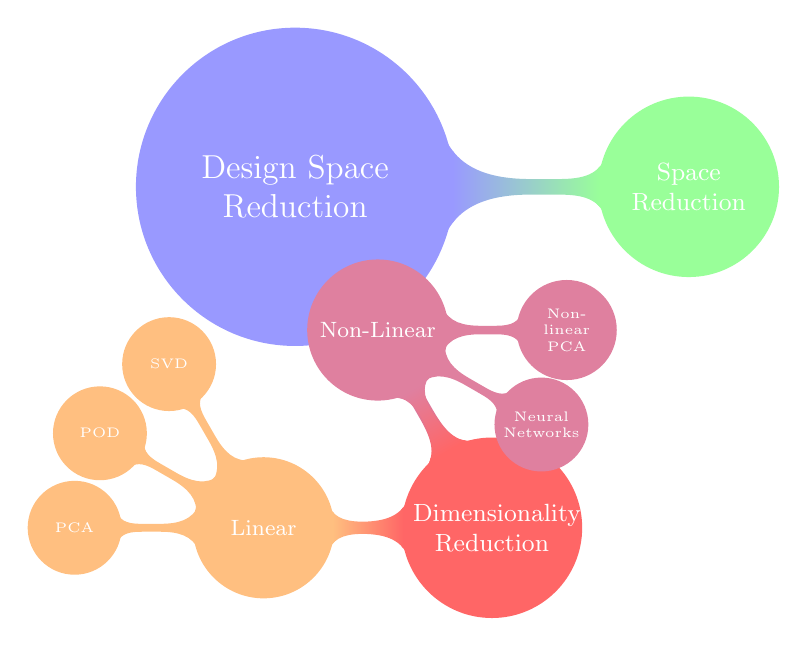
\begin{tikzpicture}
  \path[mindmap,concept color=blue!40,text=white]
    node[concept] {Design Space Reduction}
    [clockwise from=0]
    child[concept color=green!40] { 
        node[concept] {Space Reduction} 
    }
    child[concept color=red!60] {
        node[concept] {Dimensionality Reduction}
        [clockwise from=180]
        child[concept color=orange!50] {
            node[concept] {Linear}
            [clockwise from=180]
            child { node[concept] {PCA} }
            child { node[concept] {POD} }
            child { node[concept] {SVD} }
        }
        child[concept color=purple!50] {
            node[concept] {Non-Linear}
            [clockwise from=0]
            child { node[concept] {Non-linear PCA} }
            child { node[concept] {Neural Networks} }
        }
    };
\end{tikzpicture}
\caption{Overview of Design Space Reduction Techniques}
\end{figure}

In this research, we focus on the approach of dimensionality reduction as an enabler for more efficient design space exploration, possible even in the absence prior knowledge of the application or definitive design objectives. This ensures that early design stages are not bottlenecked by the need to make discrete decisions thus enabling complete design freedom. Reducing the dimensionality of the design space is is pertinent to engineering applications such as complex turbo machinery components whereby there may be 100s, or 1000s of design parameters describing the complex geometries and it may not always be possible or efficient to apply definitive constrains to all such variables particularly if pursuing completely novel designs.

We can further categorise dimensionality into two distinct approaches: linear and non-linear. Linear techniques, such as principal component analysis (PCA) and proper orthogonal decomposition (POD), are employed to reduce the dimensionality of high-dimensional design spaces.  \citep{Diez2024}. Linear approaches can yield undesirable results when simulating highly non-linear phenomena \citep{Deshpande2024} such as those typically found between engineering design parameters, therefore motivating the necessity to explore non-linear dimensionality reduction techniques \citep{Diez2024}. For example, PCA involves a linear transformatoin of features in the original data onto a new basis \citep{Donnelly2024} by searching for orthogonal directions that explain the variance in the data as much as possible - variations of PCA are explored in \cite{Sorzano2014}. Further, while PCA is a common dimensionality reduction technique, it also suffers from computational costs in high-dimensional spaces \citep{Donnelly2024} and therefore in itself can be computational bottlenecks.

More recently, machine learning has fuelled a new approach to overcoming the challenges associated with ubiquitous, high-dimensional data and offers a means for scalable, flexible and rapid dimensionality reduction all whilst being computationally inexpensive at the point of prediction \citep{Deshpande2024}, making them particularly amenable to use cases where real-time deployment is required.  Some machine learning algorithms offer a probabilistic approach to problem solving such as the variational auto encoder, allowing them to be used in downstream applications such as uncertainty quantifications of the predictions \citep{Donnelly2024}, but also in a generative sense by sampling from a learned distribution. Representation learning, referring to machine learning algorithms that learn informative features that input data inform downstream applications for tasks such as regression or classification \citep{Bengio2012}, has seen the extension to dimensionality reduction techniques that are capable of learning a compressed latent representation of otherwise high-dimensional input data, and subsequently being able to reconstruct back to the original space via an encoder-decoder type architecture that learns by iteratively measuring the difference in the original and reconstructed outputs \citep{Huang2022} and informing an update to the model weights via the process of back propgation. The two constituent parts of such model, the encoder and decoder are trained in an end-to-end loop, with a bottleneck layer which provides a compressed, lower (than the original) dimension of the data. We can denote the encoder as  $g_\phi$ and decoder as $f_\phi$ with a bottleneck layer having lesser dimensions than the original \citep{DAgostino2018}. It is this characteristic of the AE that is leveraged in downstream applications for design optimisation since the once high-dimensional design space is now represented in this new, low-dimensional latent manifold making it more suitable for dimensionally-sensitive computational tasks.

In designing an appropriate dimensionality reduction approach, the end use-case must be considered. In the context of this research, the objective is to enable efficient sampling and exploration of the design space to enable optimisation approaches such as the genetic algorithm (GA) to find, in a reasonable number of evaluations with a small starting population, an optimal solution to a performance objective. Consequently, the learned low dimensional representation must provide meaningful, compliant designs across a latent space that is continuous and smooth. Continuous and smooth referring to continuous mappings from the latent space to the original space absent of local jumps, with few high-frequency variations across the latent space \citep{Danhaive2022}. These characteristics enable interpolation within the learned latent representation to discover and generate novel, but realistic designs. However, the vanilla variant of an auto encoder is deterministic, and aims to take as input $x$ and output $x'$ by simply learning to minimise a reconstruction error, while encoding the original $x$ in a latent vector $\textbf{z}$. A standard autoencoder approach neglects any learning effort on ensuring that this latent space is smooth, therefore limiting it's use in performance optimisation frameworks. To overcome this limitation, variational autoencoders \citep{Kingma2013}, a type of generative model \citep{Danhaive2022}, introduce a regularisation during training that enforces that the latent features are form a multivariate Gaussian distribution resulting in a continuous performance surface \citep{Huang2022}. In the following subsections, we will outline the mathematical intuition behind both the vanilla autoencoder and the probabilistic extension, the variational autoencoder.

\subsubsection{Autoencoder (AE)}
An autoencoder is an supervised neural network that aims to learn to reconstruct it's inputs as accurately as possible. The latent vector that is created in the bottleneck layer of the autoencoder is a compressed representation of the original input. The dimension of this latent vector is chosen by balancing the trade-off between reconstruction error and reduction in the dimensionality required for downstream applications. For example, \cite{Donnelly2024} find that a latent vector of 12 is suitable for their application of weather forecasting using Gaussian processes. Generally speaking, as the dimension of the latent vector approaches the dimension of the original input the reconstruction error tends towards 0, however does not benefit from any dimensionality reduction, whereas large latent vectors are more expressive and retain more of the salient information yet risk failing to effectively compress the design space dimensionality to enable efficient sampling and exploration.

The autoencoder can be formulated as follows:
\begin{itemize}
  \item \textbf{Encoder:} \( g_{\phi}: \mathbb{R}^D \rightarrow \mathbb{R}^d \), which maps the input \( \mathbf{x} \in \mathbb{R}^D \) to a latent representation \( \mathbf{z} \in \mathbb{R}^d \):
  
  \begin{equation}
      \mathbf{z} = g_{\phi}(\mathbf{x})
  \end{equation}
  
  \item \textbf{Decoder:} \( f_{\phi}: \mathbb{R}^d \rightarrow \mathbb{R}^D \), which reconstructs the input from the latent representation:
  \begin{equation}
    \mathbf{x}' = f_{\phi}(\mathbf{z}) = f_{\phi}(g_{\phi}(\mathbf{x}))
  \end{equation}
\end{itemize}




The autoencoder is trained to minimize the reconstruction loss between the input \( \mathbf{x} \) and its reconstruction \( \mathbf{x}' \). A common loss function is the mean squared error (MSE):
\begin{equation}
    \mathcal{L}(\phi) = \frac{1}{N} \sum_{i=1}^N \left\| \mathbf{x}_i - f_{\phi}(g_{\phi}(\mathbf{x}_i)) \right\|^2
\end{equation}


\subsubsection{Variational Autoencoder (VAE)}
While the autoencoder provides a single output of a latent vector $z$ for a given input $x$, the variational autoencoder, a type of generative model outputs the mean vector $\mu$ and standard deviations $\sigma$ vector of the latent distribution, unlike a vanilla VAE that outputs a deterministic mapping from the original input to the latent vector. During training time, a latent vector is sampled from this multivariate latent distribution and decoded to the output, $x'$ Repeated sampling from this distribution yields different latent vectors. Rather than guiding the model training via a measurement measuring only the reconstruction loss (MSE), a regularisation term, the Kullback-Leibler divergence, is included in the loss function that measures the difference between the learned distribution and the standard normal distribution \citep{Huang2022}, this ensures that latent space is continuous and complete \citep{Lew2021}. This can be seen denoted as $D_{KL}$ in equation~\eqref{VAE loss function}. One of the key benefits to the VAE over a standard AE is that samples can be made from the latent distribution to generate new data \citep{Danhaive2022}, which in this research refers to generating new designs. It is this characteristic that enables it be used to design exploration and optimisation workflows by sampling novel designs from the latent distribution, we can identify new designs through a continuum of the design space in this low-dimensional latent manifold and since the latent space is continuous we can interpolate through this space, generating new designs every time the interpolated latent vector is decoded back to the original dimensions.

A unique feature and therefore approach for training a probabilistic variational auto encoder emerges. One of the challenges associated with training a VAE is that we cannot simply back propagate a stochastic neural network node, therefore to enable compatability with typical machine learning training approaches, \cite{Kingma2013} proposes what is denoted the \textit{reparametrisation trick}, referring to a change of the variables \citep{Kingma2019}. The intention here is to remove the stochastic nature of the sampling node, i.e., the one preventing the gradient from being computed, and instead shifting it to another differentiable random variable, $\epsilon$, where the distribution of this random variable is independent of the input $\textbf{x}$ or the encoder parameters, $\phi$. For the purpose of this research, the details are not important (refer to \citep{Kingma2013}, however, it is the reparametrisation that enables the training of a VAE similar to that of a deterministic model. A noteworth requirement for successful VAE utilisation in generative workflows, is that the data used to train the VAE should reflect realistic, and valid design points. This is important due to the way the VAE learns, specifically, that is will learn distributions around the training data that should similarly resemble the original data distribution where introducing unphysical designs would result in unphysical generated designs also \citep{Huang2022}. In this research, we opt to train the VAE on data samples from pre-defined classes of shapes that exist in the real-world, complimented by random rotations and skewing to augment the data and encourage diversity in the learnt features.

The constituent parts of the Variational Autoencoder are as follows:

\begin{itemize}
  \item \textbf{Encoder:} The encoder maps an input \( \mathbf{x} \in \mathbb{R}^D \) to the parameters of a probability distribution over the latent variables. Typically, it outputs the mean vector \( \boldsymbol{\mu} \in \mathbb{R}^d \) and the standard deviation vector \( \boldsymbol{\sigma} \in \mathbb{R}^d \) of a Gaussian distribution:
  \begin{equation}
  (\boldsymbol{\mu}, \boldsymbol{\sigma}) = g_{\phi}(\mathbf{x})
  \end{equation}
  
  \item \textbf{Latent Sampling:} A latent vector \( \mathbf{z} \in \mathbb{R}^d \) is sampled from the Gaussian using the reparametrisation trick:
  \begin{equation}
  \mathbf{z} = \boldsymbol{\mu} + \boldsymbol{\sigma} \odot \boldsymbol{\epsilon}, \quad \boldsymbol{\epsilon} \sim \mathcal{N}(\mathbf{0}, \mathbf{I})
  \end{equation}
  where \( \odot \) denotes element-wise multiplication.
  
  \item \textbf{Decoder:} The decoder maps \( \mathbf{z} \) back to the reconstructed input \( \mathbf{x}' \in \mathbb{R}^D \):
  \begin{equation}
  \mathbf{x}' = f_{\theta}(\mathbf{z})
  \end{equation}
\end{itemize}

The VAE is trained by minimizing the following loss function, which combines the previous MSE loss and a regularisation term (the Kullback-Leibler divergence between the approximate posterior and the prior):

\begin{equation}\label{VAE loss function}
\mathcal{L}(\theta, \phi; \mathbf{x}) = \mathbb{E}_{q_{\phi}(\mathbf{z}|\mathbf{x})} \left[ \log p_{\theta}(\mathbf{x}|\mathbf{z}) \right] - D_{\text{KL}} \left( q_{\phi}(\mathbf{z}|\mathbf{x}) \, \| \, p(\mathbf{z}) \right)
\end{equation}

Here:
\begin{itemize}
  \item \( q_{\phi}(\mathbf{z}|\mathbf{x}) = \mathcal{N}(\mathbf{z}; \boldsymbol{\mu}, \operatorname{diag}(\boldsymbol{\sigma}^2)) \) is the approximate posterior
  \item \( p(\mathbf{z}) = \mathcal{N}(\mathbf{0}, \mathbf{I}) \) is the prior
  \item \( p_{\theta}(\mathbf{x}|\mathbf{z}) \) is the likelihood modeled by the decoder
\end{itemize}

\subsection{Related Works}
The literature presents a vast application of generative models for the purpose of enabling dimensionality reduction to support efficiencies and maximise utilisation in downstream workflows. As is leveraged in this research, numerous studies incorporate variational autoencoders to provide a generative, continuous and smooth latent representation of an otherwise high-dimensional problem. In \cite{Huang2022} build a variational autoencoder network to compress their hardware accelerator design problem. The specific problem focuses on a discrete design space, including variables such as number of processing elements, resulting in a large but finite design space of $10^{17}$ configurations over 6 discrete parameters. In the 2D domain of geometric shape optimisation, this design landscape is continuous and infinite, therefore reinforcing the necessity to provide a compact representation over which to search. In addition to transforming their design representation, they also develop a predictive model for latency and energy predictors, performing as a surrogate model. Due to the analytical tractability of our performance metric, we opt to compute the performance surface directly. The VAE model and fully connected multi-layer perceptron (MLP) are trained in an end-to-end manner thus providing a combined loss for the training process that includes the VAE loss, and the loss associated with the energy and latency predictions. By incorporating a fully differentiable MLP network, they also enable gradient determination via auto-differentiation to provide a performance function over the latent space, making it interfaceable with gradient based optimisation techniques. While the study makes acknowledgement to training the models on realistic and valid data points in the design space, they do not demonstrate the inability of performing optimisation methods on their original design manifold containing 6 design variables. Our work aims to motivate the need for pursuing low-dimensional representations by performing geometric shape optimisation on geometries in a high-dimensional representation and compare the efficacy when performed post-latent transformation. Similarly to our work, the authors demonstrate the reconstruction loss of the VAE over 4 different latent dimensions (i.e., [1,2,4,6]). Metrics for assessing their models include finding the highest performing points, and sample efficiency defined as the rate at which optimisation frameworks find points in the latent design space that have a performance within 3\% of the highest known. Finally, the authors also opt to explore different values for the Beta term, controlling the weighting of the KL-divergence in the combined VAE loss term to assess performance at Beta=0, 0.01 and 0.0001. We do not apply any weighting to KL-divergence component of the VAE loss term in order to minimise the number of independent variables between the different VAE models, with the intent of providing unbiased insights into impact of adjusting only the bottleneck size of our network.

Andrew Lew et al also employ VAEs to enable efficient design space exploration, with a focus on material structures, especially for optimisation of cantilever design via trajectory exploration within the 2D latent space. Their use of a VAE model enables exploration and generation of novel cantilever designs, thus unveiling performant designs extrapolated beyond the limits of the original training dataset. They opt to use image data as their input into the models, whereby each datapoint into the VAE is an image of a cantilever design with a varying mass fraction between 5\% and 99\%. By utilising an image-based format of their data, they can leverage 2D convolutional operations (Oshea CNNs) for the VAE architecture, thus enabling the learn of spatial features in the dataset in the form of convolutional filters. Such an architecture is an efficient alternative to the fully connected MLP due to the weight sharing nature of the convolutional filters, making it well-suited to high-dimensional computationally expensive input data. While the author reports 2D input images, convolutional approaches can be extended to 3D convolutions where features are learned from voxels. While this approach is promising, opting to represent inputs as 2D pixel or 3D voxel images enforces a loss of fidelity, whereby the inputs are constrained to a discretised grid. While doing this does reduce the design space volume from continuous to discrete, it introduces a loss of fidelity and therefore information. For example, attempting to represent a highly complex curved surface via pixels will introduce steps to the surface, therefore detracting from the original high-fidelity input. In our research, we maintain a more typical  representation of the geometric shapes defined by nodes on a 2D manifold with fixed connectivity denoting the boundaries of the 2D shapes, which is easily extensible to 3D geometry representations (defined by nodes and edges).



\newpage

\section{Methodology}
As part of this research, we investigate methods that enable a more controllable and efficient approach to design space representation, exploration and optimisation. The overall objective of this research will be to investigate and implement an approach for reducing the complexity of engineering design space problems to enable efficient design space exploratoin to better service downstream applications such as design optimisation or uncertainty quantification. To formalise this, there are 3 research objectives that direct the research efforts as follows:
\begin{enumerate}
    \item Investigate techniques and approaches for representing geometry in a low dimensional form to enable sample efficient design space optimisation and carry out a comprehensive literature review of existing methods, to both the representation problem, and design space exploration and optimisation.
    \item Develop approaches for representing 2D geometries in a lower dimensional representation that can be used directly as part of a geometric shape optimisation problem and investigate the structure and smoothness of the learned geometry representations and their suitability for use in different optimisation approaches.
    \item The research will assess which approaches to geometry representation provide the most interpretable and controllable representation that can be harnessed to conduct targeted design modification and optimisation for the selected optimisation problem.
\end{enumerate}

In accordance with the above, this research will provide both a theoretical investigation of novel data-driven methods for representing complex design problems in a low-dimensional, sample efficient format, but will also include the development of and testing of the identified approach as part of an engineering design optimisation problem. Specifically, the method will be used to optimise 2D shapes for a metric denoted as compactness as defined in Equation~\eqref{eq:compactness}. To motivate the investigation, a demonstration of the challenges associated with performing design space exploration in high-dimensional parametrised spaces will be conducted and then compared the results when deployed into a low-dimensional latent space. The metaheuristic approach of the genetic algorithm as described in \ref{GA} will be used to demonstrate the effect on the number of generations required, and required starting population size by transforming the problems into the latent representations of otherwise high-dimensional problems that quickly fall victim to the curse of dimensionality.

The workflow can be categorised into two main parts, firstly, the development and training of a dimensionality reduction technique that can ingest high-dimensionally represented 2D shapes, and learn a concise low-dimensional representation. In this research, we focused on a probabilistic deep learning model, the variational autoencoder (VAE) which is an extension of the deterministic autoencoder (AE) to enable a smooth, continuous latent space that enables interpolation for design optimisation and discovery. The second part is the integration of the learned representation into an optimisation framework that enables directed evolution towards an optimal solution according to our defined fitness function (i.e., the compactness metric) for which to optimise. The VAE is trained separately to the deployment into the optimisation framework in order to generate a latent space dataset that can be used in downstream applications, such as as part of a genetic algorithm \citep{Deshpande2024}. The complete workflow is shown in Figure~\ref{VAE_GA_workflow}, denoting the separate VAE and GA. The VAE is trained in isolation to the VAE, however, the train model is used inside the GA loop to transform from the low-dimensional latent representation to the original shape structure for the purpose of computing the area, perimeter and therefore compactness. The final selected designs, according to those with optimal fitness values, are decoded at the final stage.


\begin{figure}[htp]
    \centering
    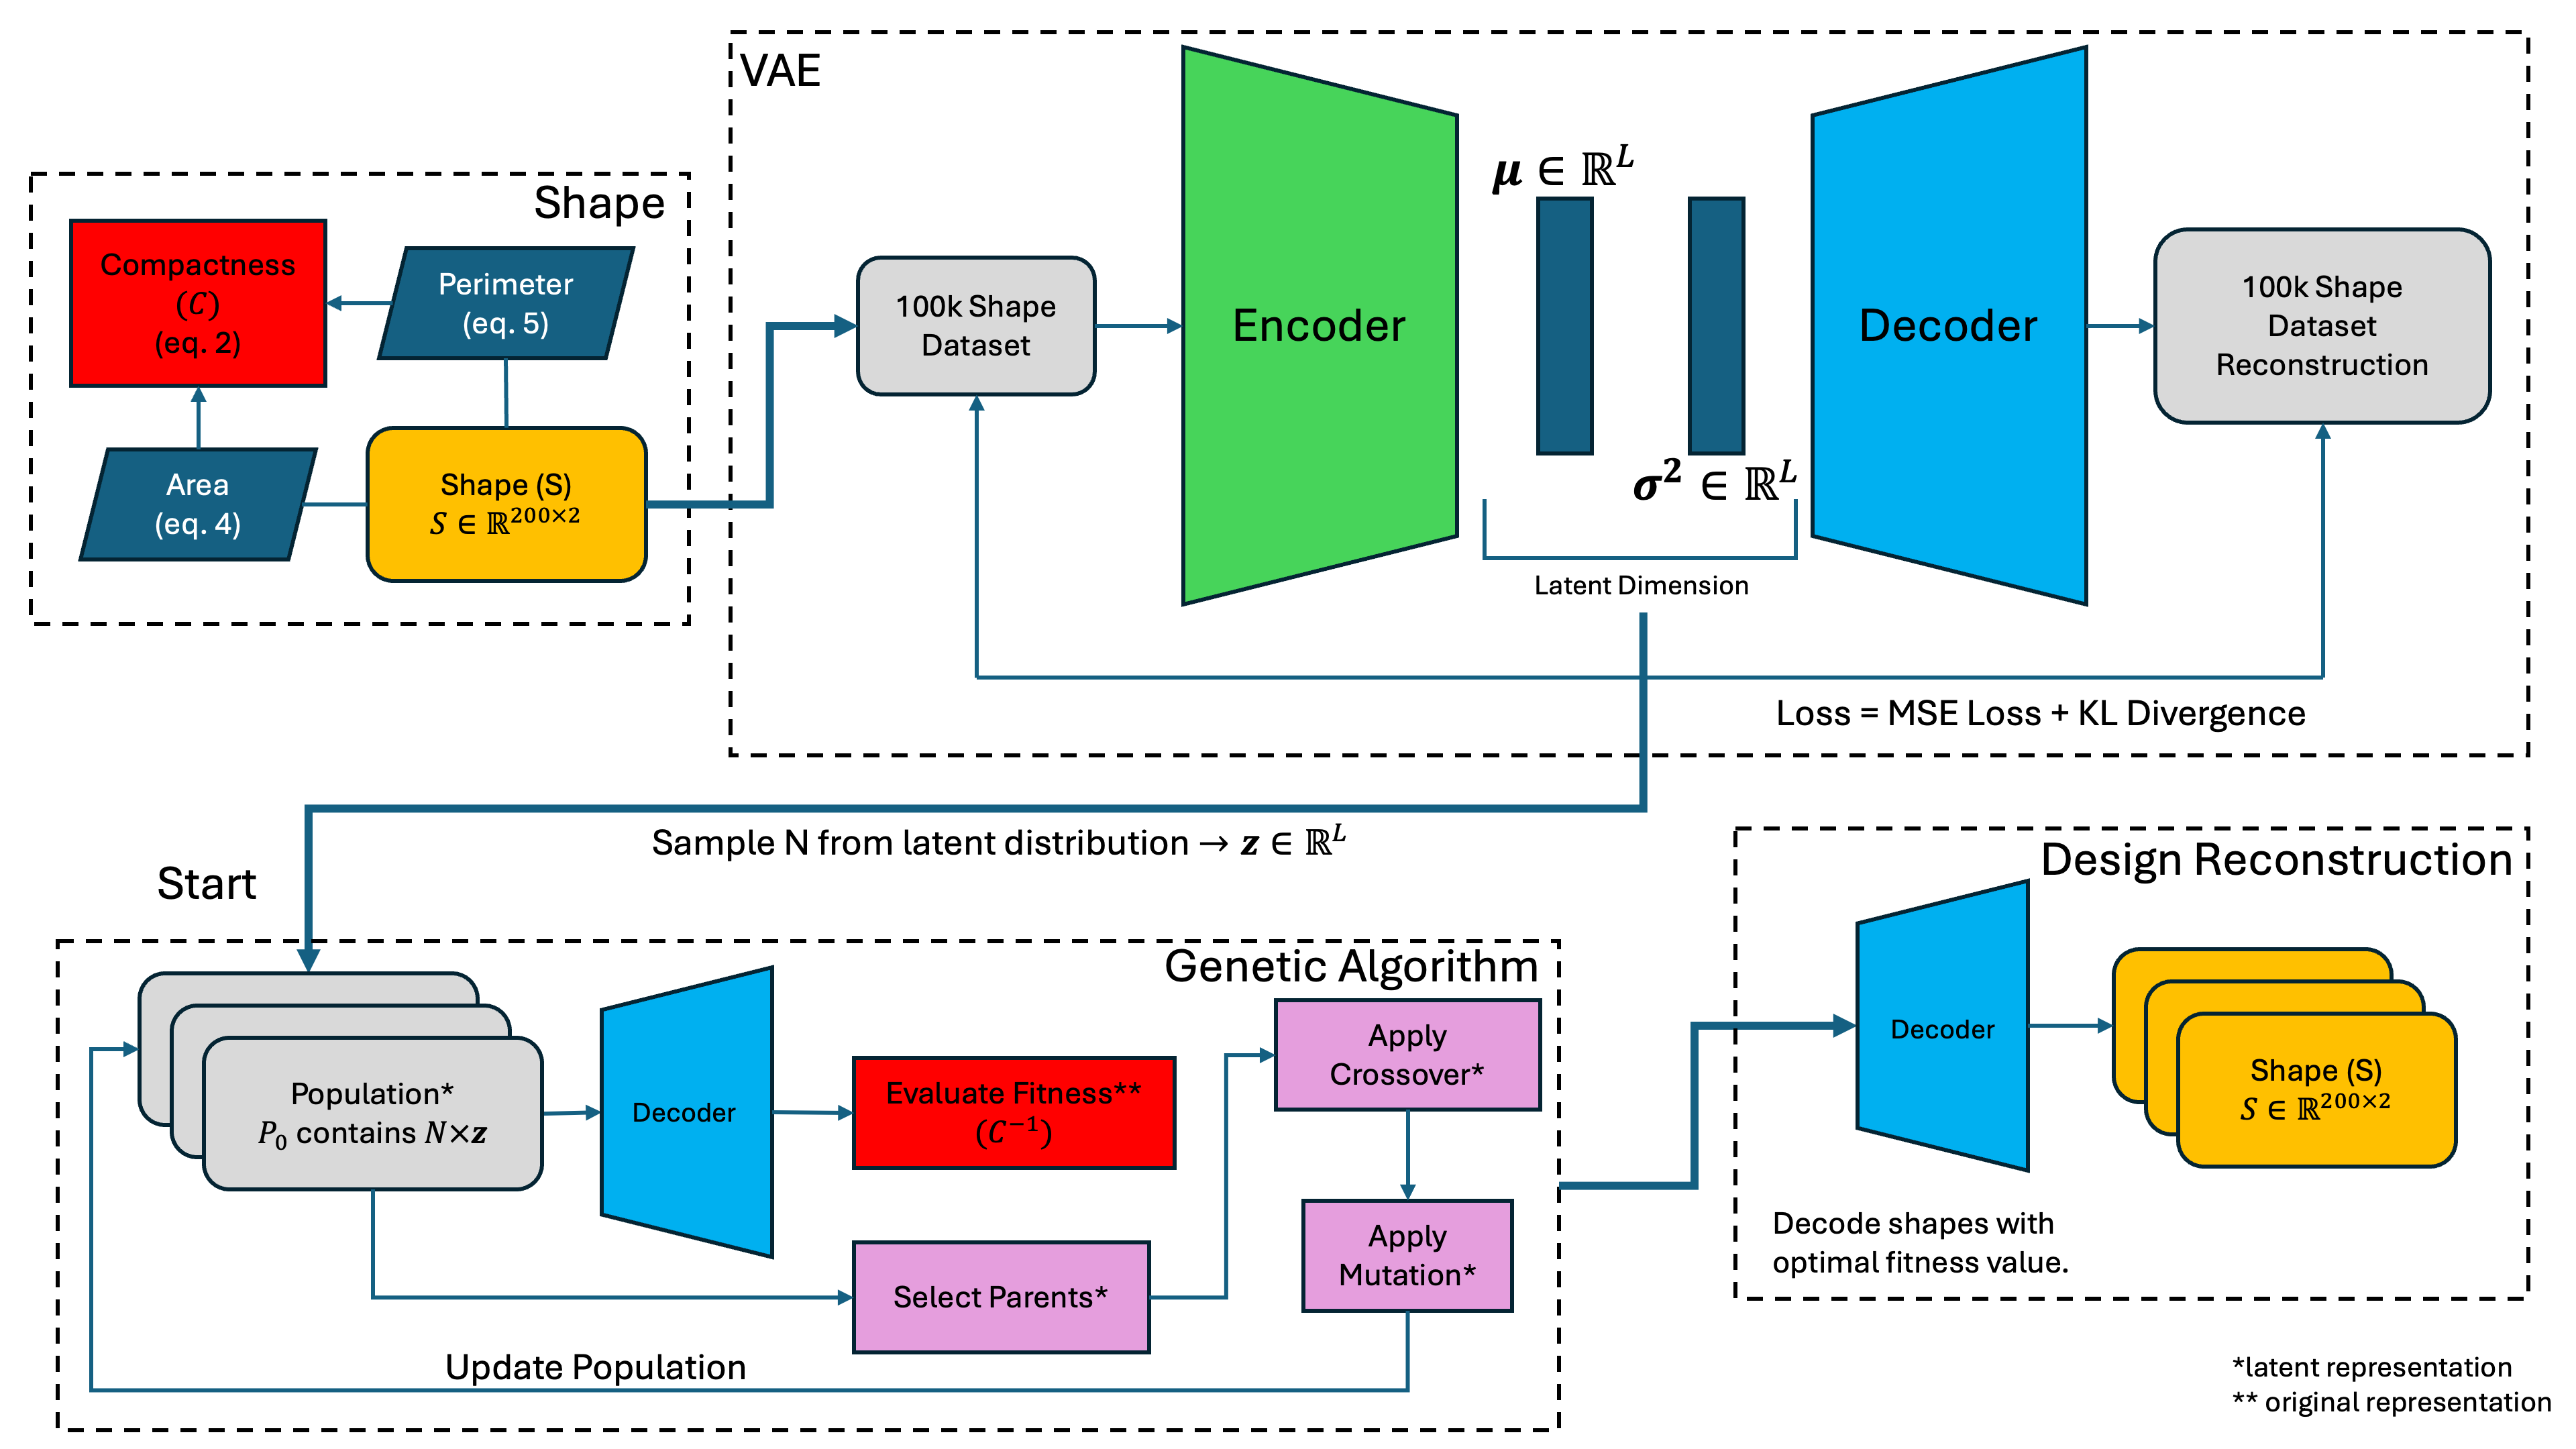
\includegraphics[width=12cm]{figures/workflow_diagram.png}
    \caption{Combined VAE and GA optimisaton workflow}

    \label{VAE_GA_workflow}
\end{figure}





\subsection{Hypothesis}

Due to the challenges posed by high-dimensional problems, the hypothesis of this research is that by employing data-driven methods to provide a reduced dimensionality representation,  the design space will be more efficiently accessible without having to iterate over a high number of combination of design parameters and therefore, the number of evaluations of samples from the design space will be reduced in order to obtain an optima. 
Additionally, some generative models such as variational autoencoders result in a latent design space that is continuous, which is one of the requirements to employ optimisation techniques such as gradient based methods \citep{Archbold2024}, which also require the objective function to be analytically or numerically differentiable. We hypothesise that approaches such as the genetic algorithm will converge with a smaller number of starting samples, and in fewer generations than if performed in the high-dimensional space. This is significant in engineering design, since the evaluation of samples in the design space is often expensive, therefore a limited number of initial samples in the population is probable, and being able to perform numerous re-evaluations during each generation may be intractable in expensive engineering workflows. The difference between performing 5 or 10 performance evaluations via costly CFD may mean the difference between identifying or missing a performant novel design. We also hypothesise that by employing a variational autoencoder as the dimensionality reduction technique, there will be a loss of information attributed to the compression in the latent layer and the probabilistic nature of the latent distribution. However, the generative nature of the VAE should enable the creation of realistic/logical designs that closely match the original dataset, although the absolute reconstruction of any particular shape (i.e. $\textbf{x} \rightarrow \textbf{z} \rightarrow \textbf{x'}$) will likely demonstrate heightened reconstruction losses. To overcome this, a deterministic approach via a vanilla autoencoder may be employed resulting in a deterministic reconstruction of $\textbf{x}\rightarrow\textbf{z}\rightarrow\textbf{x'}$, though this would not favour interpolation and exploration through the latent space since there is no constraint on the generated latent space to ensure a smooth and continuous manifold, thus limiting the use case to dimensionality reduction and not discovery of new designs. In the workflow shown in Figure~\ref{VAE_GA_workflow}, the trained VAE is used only for it's decoder in converting the evolved latent dimensions back to the original dimension to enable the performance evaluation to be conducted. Since the latent values are generated via exploration, and not a result of inputting a predefined shape $\textbf{S}$ into the trained encoder $g_\phi$, the operation of decoding is isolated with no ground-truth measure to compare against. Instead, the compactness metric is computed in the high-dimensional space thus informing which of the individuals in the GA population to select for the next generation, therefore the actual shape that is reconstructed is not important as the GA will evolve towards those with the highest fitness values.

\subsection{Data}
By design, this research has been conducted in a way that abstracts the underlying concepts from the necessity of complex, IP-sensitive datasets common to modern engineering applications. The downstream use case of methods explored in this research may include sensitive commercial designs that would not be easily permitted for the public domain, such as aerodynamic profiles of jet turbine airfoils. However, the purpose of this research is not to provide a deterministic means for design engineers to optimise specific components, rather to identify, investigate and highlight the benefits and limitations realised by data driven methods in enabling design space exploration workflows, agnostic of the specific use-case. We employ the philosophy that in demonstrating the efficacy of an approach, a suitable level of abstraction should be used to simplify the problem to it's core principles - this aligns with Ocams razor 'entities should not be multiplied beyond necessity' \citep{Gori2024}. For this reason, we restrict the research to focus on 2-dimensional shapes, represented as a series of nodes defined by coordinates in the 2D manifold with fixed connectivity. While providing a simplification benefit in terms of computational cost and memory requirements, it is not difficult to extend the concepts to the commonly used 3D representation in engineering designs (see Section~\ref{Geometry}). By abstracting the data requirements to this level, we avoid distracting from the underlying principles in the techniques, and enable an unbiased assessment free of complex failure behaviour influenced by
multiple factors that might not be apparent, as is typical in industrially relevant applications \citep{Hobbs2021}.

In some engineering applications, training data-hungry machine learning models is often intractable due to the volume of data required to reach an appropriate accuracy, particularly if obtaining the data is not trivial and burdened by some significant computational investment. For example, if trying to construct a data-driven model that is able to predict steady-state flow approximations in the field of fluid dynamics, it is required that computationally expensive computational fluid dynamics (CFD) simulations are performed across a vast design space to obtain a suitable voluminous training dataset. Such an approach to acquisition of data is computationally intensive, and can take hours or days in some cases for complex prototypes \citep{guo2016convolutional}. The case-study in this research does not suffer from such challenge, attributed to the accessibility of evaluating the performance metric analytically (see Equation~\ref{eq:compactness}).
The use of a VAE does necessitate a significant training dataset size to effectively capture and learn the features necessary to construct a low-dimensional representation that also enables reconstruction to the original manifold. We opt for the creation of a 100,000 random shape dataset composed of triangles, squares, rectangles, hearts, stars, pentagons and diamonds. All shapes are normalised to have x,y values between [0,1] in both the x and y dimensions. The shapes are defined by a series of 200 nodes each of x,y position as described in Section~\ref{Geometry}. The shapes are also randomly rotated and skewed to add additional variability into the dataset, with the intention of expanding the variation of features present during training to aid in generalisability of the trained VAE. Some examples of the training data used in training the VAE are shown in Figure~\ref{fig:vae_Shapes}. An important consideration when training a VAE for the purpose of reconstruction and generation is that only valid design points are used, that is, designs that are realistic in the context of the application \citep{Huang2022} as to promote the VAE to learn a distribution of valid designs. For this reason, we provide realistic shapes from defined categories to reflect this valid design landscape. In engineering applications, this may correspond to providing only physical designs that satisfy specific constraints, such as those defined in typical engineering standards for structural designs. The alternative approach may include providing shapes defined as random noise into the VAE - however, the learned distribution of the data would result in the generation of a distribution that matches the original and hence generate noisy shapes. Such an approach may be suitable when there exists no prior engineering knowledge or intuition to direct the design landscape accordingly, rather complete freedom is sought to identify novel design cases.

Since the 100,000 random shape dataset is utilised to train a variational autoencoder (VAE) that enables a low-dimensional latent representation of otherwise 200-node 2D shapes, it is not necessary to retain this training dataset for subsequent optimisation routines. Instead, the advantage provided by the probabilistic nature of the trained VAE is that we can sample values for the latent dimensions, thereby generating novel designs. These samples can be utilised as the initial population for design optimisation frameworks. By doing so, we do not limit the design exploration to designs solely prescribed during the initial VAE training phase, but instead facilitate a comprehensive exploration across a reduced set of dimensions that, when reconstructed by the VAE decoder, correspond to the original 200-node 2D shapes. To generate the initial population for the GA shown in Figure~\ref{VAE_GA_workflow} we first encode all shapes from the original 100,00 training dataset and plot the distributions across all latent dimensions. This distribution is used to inform the bounds of latent values which form the original training data. We generate random latent values within these bounds to create an initial population for the genetic algorithm.

\begin{figure}[htp]
    \centering
    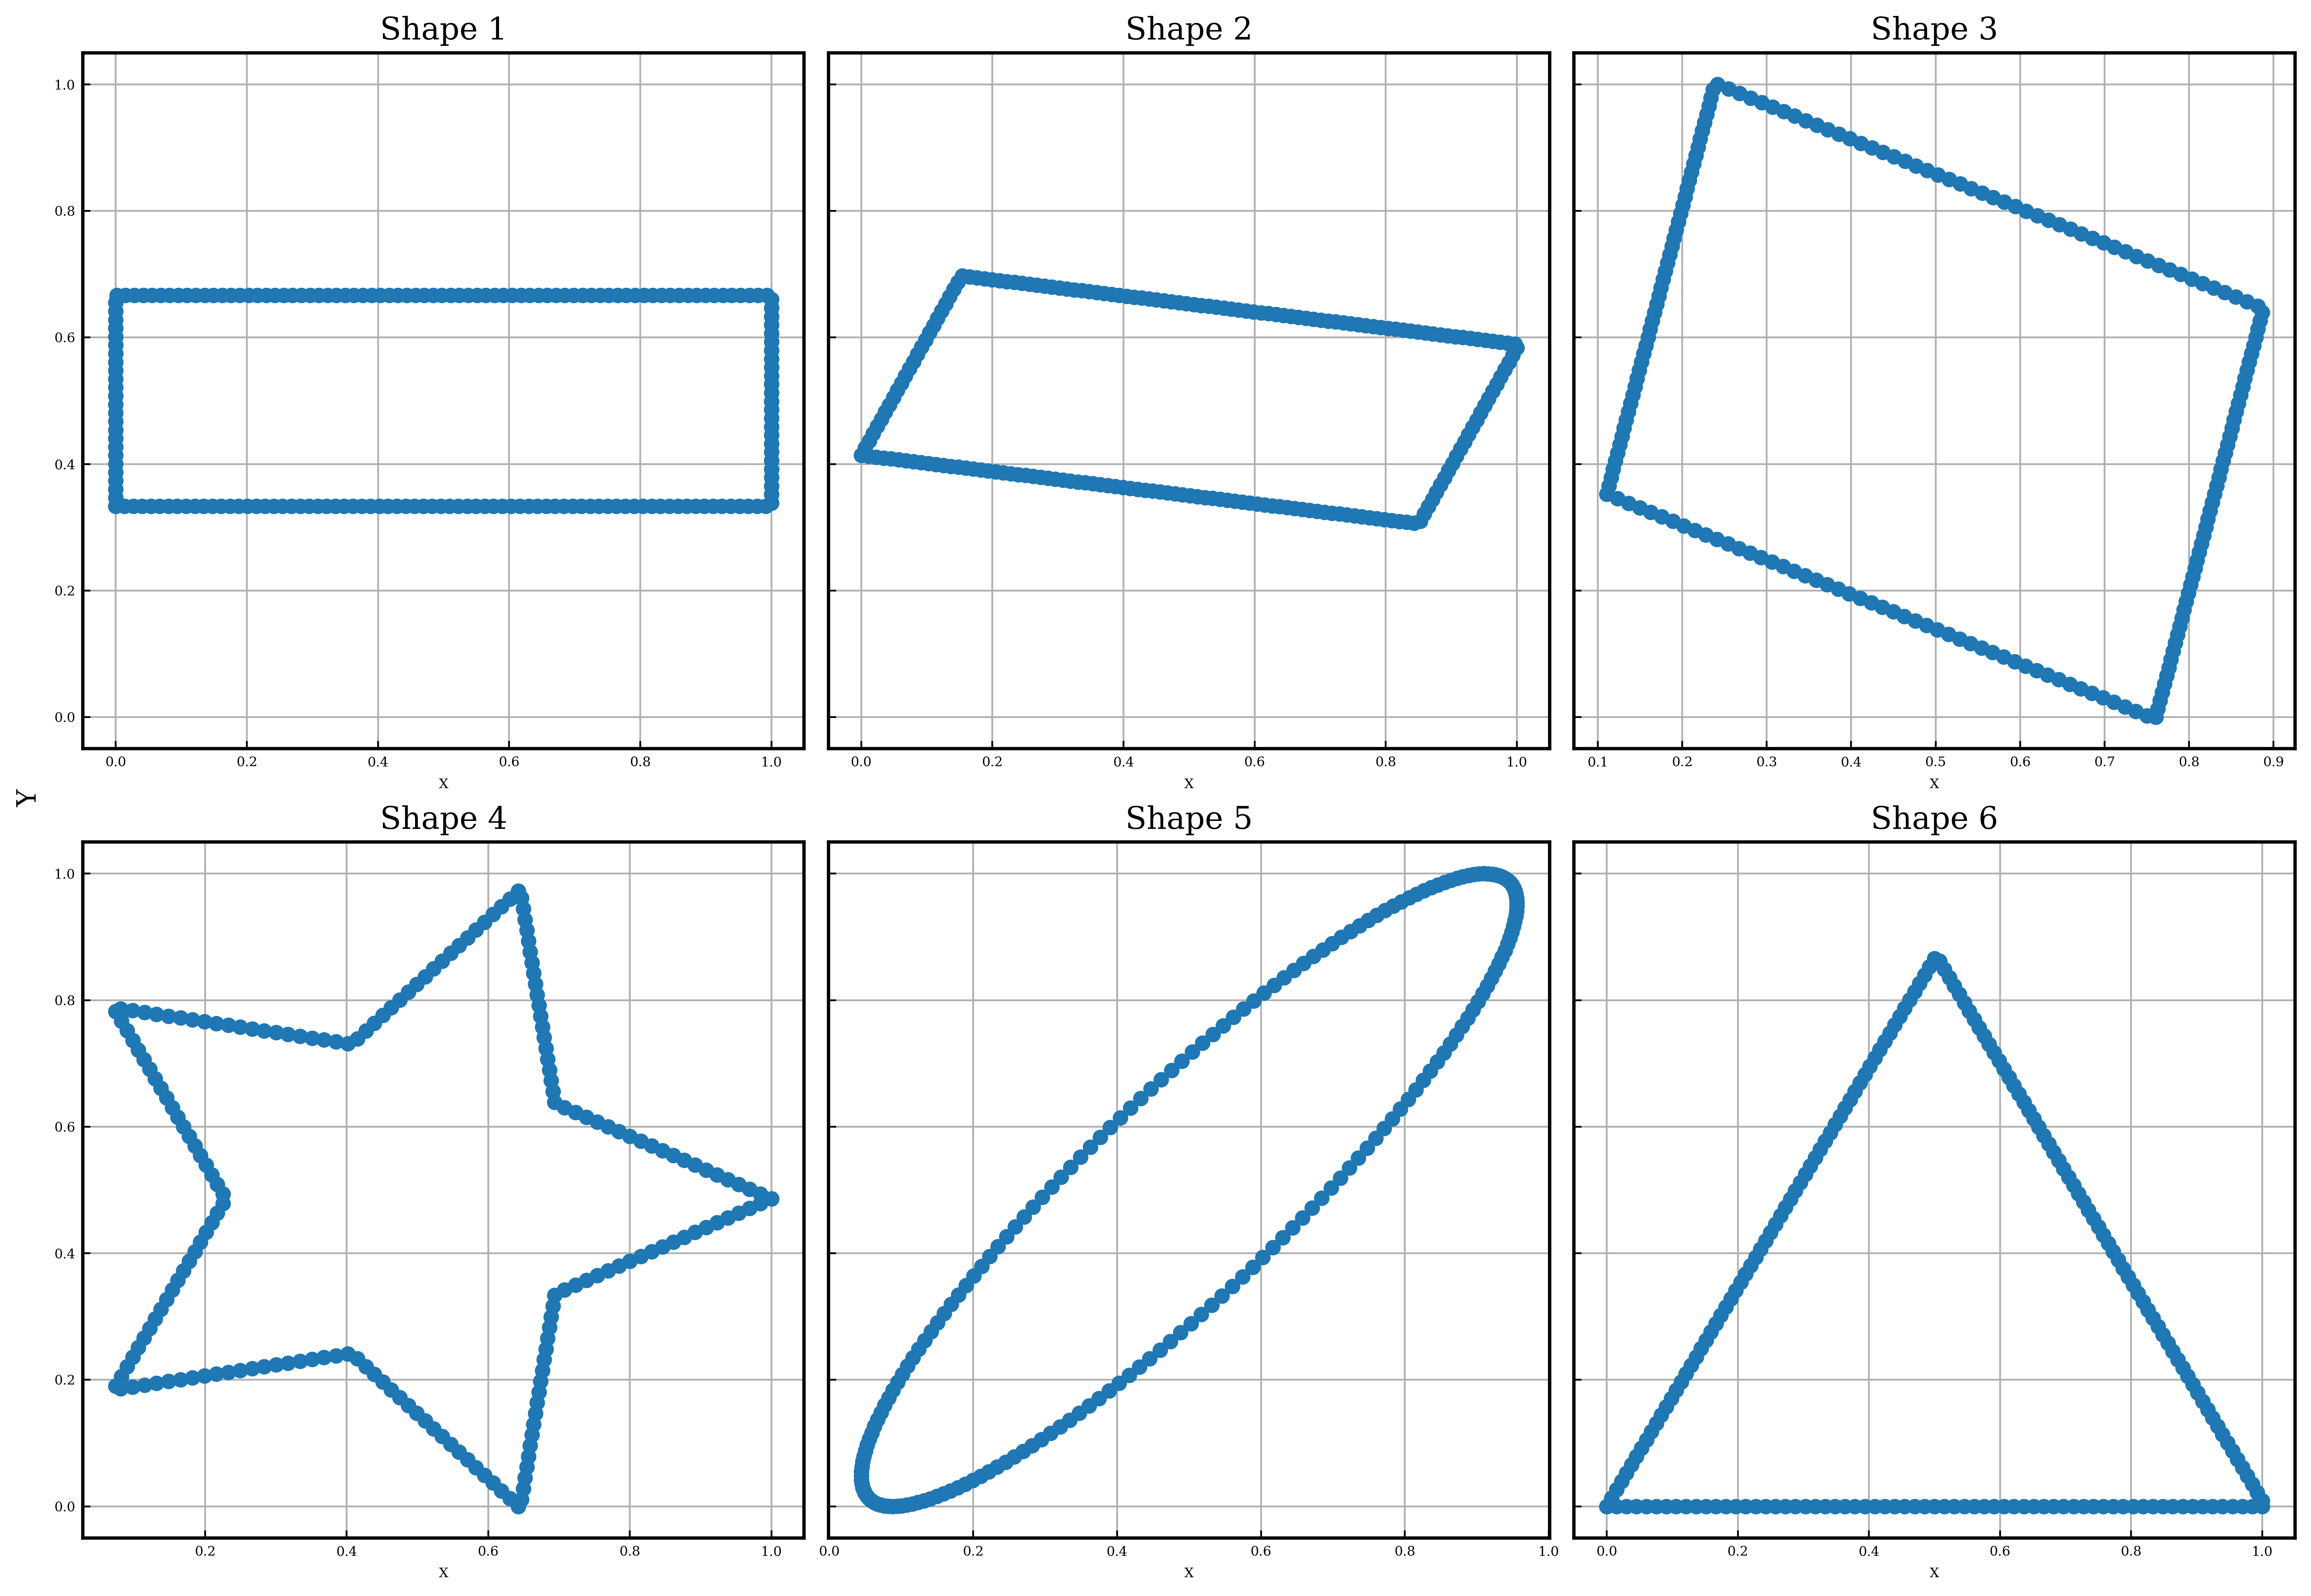
\includegraphics[width=12cm]{figures/6examples_shapes.png}
    \caption{VAE Training Dataset Example Shapes, $N=200$}
    \label{fig:vae_Shapes}
\end{figure}
\newpage{}

\subsection{VAE Model Architecture}

The Variational Autoencoder (VAE) implemented in this work is a fully connected neural network designed to encode and decode high-dimensional shape vectors into a low-dimensional latent space. The architecture is composed of an encoder network $g_\phi$, a latent space parameterisation, and a decoder network $f_\theta$.

\paragraph{Encoder Network}

The encoder maps the input vector $\mathbf{x} \in \mathbb{R}^D$ (where $D$ is the input size) into a latent space of dimension $L$ (here, $L = 2$). $\textbf{b}_1$ and $\textbf{b}_2$ are bias vectors. This is achieved through a two-layer feedforward neural network with ReLU activations:

\begin{align}
\mathbf{h}_1 &= \text{ReLU}(\mathbf{W}_1 \mathbf{x} + \mathbf{b}_1) \quad \text{where } \mathbf{W}_1 \in \mathbb{R}^{256 \times D} \\
\mathbf{h}_2 &= \text{ReLU}(\mathbf{W}_2 \mathbf{h}_1 + \mathbf{b}_2) \quad \text{where } \mathbf{W}_2 \in \mathbb{R}^{128 \times 256}
\end{align}

The output $\mathbf{h}_2 \in \mathbb{R}^{128}$ is then linearly transformed to produce the parameters of the approximate posterior distribution:

\begin{align}
\boldsymbol{\mu} &= \mathbf{W}_\mu \mathbf{h}_2 + \mathbf{b}_\mu \quad \text{where } \boldsymbol{\mu} \in \mathbb{R}^L \\
\log \boldsymbol{\sigma}^2 &= \mathbf{W}_{\log\sigma^2} \mathbf{h}_2 + \mathbf{b}_{\log\sigma^2} \quad \text{where } \log \boldsymbol{\sigma}^2 \in \mathbb{R}^L
\end{align}

\paragraph{Latent Sampling via Reparametrisation Trick}

To allow back propagation through the stochastic sampling process, the reparametrisation trick is used:

\begin{equation}
\mathbf{z} = \boldsymbol{\mu} + \boldsymbol{\sigma} \odot \boldsymbol{\epsilon}, \quad \boldsymbol{\epsilon} \sim \mathcal{N}(\mathbf{0}, \mathbf{I})
\end{equation}

where $\boldsymbol{\sigma} = \exp(0.5 \log \boldsymbol{\sigma}^2)$ and $\odot$ denotes element-wise multiplication.

\paragraph{Decoder Network}

The decoder reconstructs the input vector from the latent vector $\mathbf{z} \in \mathbb{R}^L$ using another two-layer feedforward network with ReLU activations:

\begin{align}
\mathbf{h}_3 &= \text{ReLU}(\mathbf{W}_3 \mathbf{z} + \mathbf{b}_3) \quad \text{where } \mathbf{W}_3 \in \mathbb{R}^{128 \times L} \\
\mathbf{h}_4 &= \text{ReLU}(\mathbf{W}_4 \mathbf{h}_3 + \mathbf{b}_4) \quad \text{where } \mathbf{W}_4 \in \mathbb{R}^{256 \times 128} \\
\hat{\mathbf{x}} &= \mathbf{W}_5 \mathbf{h}_4 + \mathbf{b}_5 \quad \text{where } \hat{\mathbf{x}} \in \mathbb{R}^D
\end{align}

\paragraph{Training Objective}\label{prior_dist}

The VAE is trained to minimize the standard VAE loss function, which combines the reconstruction loss (mean squared error) and the Kullback--Leibler (KL) divergence between the approximate posterior $q(\mathbf{z}|\mathbf{x})$ and the prior $p(\mathbf{z}) = \mathcal{N}(0, \mathbf{I})$:

\begin{equation}\label{eq:VAE_loss_function}
\mathcal{L}(\mathbf{x}, \hat{\mathbf{x}}, \boldsymbol{\mu}, \log \boldsymbol{\sigma}^2) = \| \mathbf{x} - \hat{\mathbf{x}} \|^2 + \frac{1}{2} \sum_{i=1}^{L} \left( \mu_i^2 + \exp(\log \sigma_i^2) - \log \sigma_i^2 - 1 \right)
\end{equation}

This encourages the network to learn meaningful, continuous latent representations while ensuring that samples drawn from the latent space produce realistic outputs.



In total, there are 5 different models trained. All models share the same architecture except for the latent dimension which is increased from 2 dimensions to 6 to expand the expressive capacity of the latent layer (see Table~\ref{tab:vae_models}). The key difference is that at the bottleneck layer there is an increasing size of the latent distributions defined by $\mu$ and $log\sigma^2$. While these vectors define a multivariate normal distribution, sampling from these distributions results in latent vectors that can be inputted into the trained decoder, $f_\theta$ to obtain a reconstructed shape, $x'\in \mathbb{R}^D$. One of the underlying assumptions in a VAE is that the covariance matrix of the multivariate Gaussian distribution in the latent layer is diagonal such that there are no correlations between latent dimensions (i.e. all off diagonal values of the covariance matrix are 0). Since the model architecture remain relatively consistent, the parameter count across the models also remains similar around 272,000 parameters. 

\begin{table}[h]
\centering
\begin{tabular}{|c|c|c|l|}
\hline
\textbf{Model} & \textbf{Latent Dimension} & \textbf{Parameter Count} & \textbf{Architecture Details} \\
\hline
Model 1 & 2 & 272{,}276 & \begin{tabular}[c]{@{}l@{}}Encoder: 400 → 256 → 128 → (2 for $\mu$, 2 for $\log\sigma^2$)\\ Decoder: 2 → 128 → 256 → 400\end{tabular} \\
\hline
Model 2 & 3 & 272{,}662 & \begin{tabular}[c]{@{}l@{}}Encoder: 400 → 256 → 128 → (3 for $\mu$, 3 for $\log\sigma^2$)\\ Decoder: 3 → 128 → 256 → 400\end{tabular} \\
\hline
Model 3 & 4 & 273{,}048 & \begin{tabular}[c]{@{}l@{}}Encoder: 400 → 256 → 128 → (4 for $\mu$, 4 for $\log\sigma^2$)\\ Decoder: 4 → 128 → 256 → 400\end{tabular} \\
\hline
Model 4 & 5 & 273{,}434 & \begin{tabular}[c]{@{}l@{}}Encoder: 400 → 256 → 128 → (5 for $\mu$, 5 for $\log\sigma^2$)\\ Decoder: 5 → 128 → 256 → 400\end{tabular} \\
\hline
Model 5 & 6 & 273{,}820 & \begin{tabular}[c]{@{}l@{}}Encoder: 400 → 256 → 128 → (6 for $\mu$, 6 for $\log\sigma^2$)\\ Decoder: 6 → 128 → 256 → 400\end{tabular} \\
\hline
\end{tabular}
\caption{Comparison of VAE models with different latent dimensions}
\label{tab:vae_models}
\end{table}

\subsubsection{Model Training}
To ensure consistency across the trained models and allow the effect of the latent dimension to be prevalent and discernible in the results, we maintain the same training parameters and process across all models. As shown in Table~\ref{tab:vae_models}, all models have similar numbers of parameters. For this reason, we maintain the same 100,000 sample training dataset for training all the VAE models. In machine learning, it is a common requirement to provide additional data as a model architecture increases significantly, however, in this research the relatively small increase in model parameters is assumed to have negligible effect on the models ability to learn. Further, we maintain a consistent batch size of 512 for the same reason. The learning rate was also fixed at $1\times10^{-3}$, and demonstrated a reasonable levels of learning via observation of the loss curves demonstrating convergence of the combined loss. All models were run for 1000 epochs, with their loss values being logged every 200 epochs. This enabled recovery of an earlier model if the final loss curve demonstrated divergence from optimal performance. The comparisons of models in this research are done at the 1000 epoch training point. The popular Adam optimiser \citep{Kingma2014} is used for the optimisation algorithm to direct the learning of the neural network weights, and is often preferred over stochastic gradient descent (SGD) attributed to it's dynamic learning rates often leading to faster convergence. Table~\ref{tab:vae_training_config} shows the hyper-paramaters used during training for each model. Finally, the rectified linear unit (ReLU) (see \cite{FredAgarap2018}) is used as the non-linear activation function for all layers except for the final layer. ReLU is defined as $\text{ReLU}(x) = \max(0, x)$, meaning all negative values are set to 0 and there is no upper bound on positive outputs. We select this activation function as all the input shapes to the VAE are scaled between 0 and 1, therefore the removal of negative values is not detrimental to the models learning.

\begin{table}[h]
\centering
\begin{tabular}{|c|c|c|c|c|c|}
\hline
\textbf{Model} & \textbf{Batch Size} & \textbf{Activation Function} & \textbf{Learning Rate} & \textbf{Optimizer} & \textbf{Epochs} \\
\hline
Model 1 & 512 & ReLU & 0.001 & Adam & 1000 \\
\hline
Model 2 & 512 & ReLU & 0.001 & Adam & 1000 \\
\hline
Model 3 & 512 & ReLU & 0.001 & Adam & 1000 \\
\hline
Model 4 & 512 & ReLU & 0.001 & Adam & 1000 \\
\hline
Model 5 & 512 & ReLU & 0.001 & Adam & 1000 \\
\hline
\end{tabular}
\caption{Training configuration for each VAE model}
\label{tab:GA_models}
\end{table}

\subsection{Genetic Algorithm}
To facilitate an intuitive and interpretable comparison of performing design optimisation in a reduce-dimension latent space, we apply the genetic algorithm to the original 200 node high-resolution 2D shapes as well as the latent-representation equivalent. We denote GAs performed on high-resolution shape data as \textbf{\textit{original}} and those performed on the low-dimensional latent representation as \textbf{\textit{latent}}. To further emphasise the effect of design problem dimensionality on the ability to perform design optimisation we apply the genetic algorithm to a population of high-resolution random shapes defined by varying numbers of nodes in 2D space with fixed connectivity. Table~\ref{tab:GA_models_original} shows all the GAs run on these high-dimensional random noise shapes. Examples are shown in Figure~\ref{fig:high_res_noise_10} and Figure~\ref{fig:high_res_noise_100}. For these cases, initial populations of the GA do not  reflect realistic points in the design space, which is one of the pre-requisite for effectively training a VAE, however, for the purpose of demonstrating dimensionality sensitivity on optimisation we opt for this initial representation.

In contrast, those used in the GAs shown in Table~\ref{tab:GA_models_latent} represent shapes drawn from the multivariate latent distribution for each of the different VAE models (see Table~\ref{tab:vae_models}) and consequently reflect shapes similar to those used in training the original VAE models (see Figure~\ref{fig:latent_shape_popM1} and Figure~\ref{fig:latent_shape_popM4}). For each of the cases in Table~\ref{tab:GA_models_latent}, we also reconstruct the initial population containing samples of $\textbf{z}$ back back to the original dimension via the \textit{decoder}, $f_\theta$, such that $f_\theta(\textbf{z)}\rightarrow\textbf{x'}$ and then apply the genetic algorithmn in this manifold (i.e., $\textbf{x'}\in \mathbb{R}^{200}$). By projecting back to the high-dimension and applying the genetic algorithm we obtain a direct indication of the efficiency gain enabled by performing the optimisation workflow in reduced dimensions. Further, by comparing the GA performance across the different dimensional latent spaces models, we also see the effect of adding additional latent-dimensions to the GA performance.

The demonstration of the GA in the original high-dimensional space acts as motivation for pursuing a low-dimensional representation to overcome the curse of dimensionality, reduce the number of evaluations required to effectively cover a design space and ultimately converge towards an optimal solution more efficiently. In the results section, we provide examples of the initial starting populations for both problem domains (high-resolution \& latent), and the consequential effect on the ability to find an optimal solution in context of the compactness objective function.

\begin{figure}[h]
    \centering
    \begin{subfigure}[b]{0.45\textwidth}
        \centering
        \includegraphics[width=\textwidth]{figures/random_noise_shapess/100point_initial_pop.png}
        \caption{$N=100$, GA5}
        \label{fig:high_res_noise_100}
    \end{subfigure}
    \hfill
    \begin{subfigure}[b]{0.45\textwidth}
        \centering
        \includegraphics[width=\textwidth]{figures/random_noise_shapess/10point_initial_pop.png}
        \caption{$N=10$, GA1 \& GA2}
        \label{fig:high_res_noise_10}
    \end{subfigure}
    \caption{Original representation random noise example shapes for GA initial population (Table~\ref{tab:GA_models_original})}
    \label{fig:random_noise_ga_shapes}
\end{figure}

\begin{table}[h]
\centering
\resizebox{\textwidth}{!}{%
\begin{tabular}{|c|c|c|c|c|c|c|}
\hline
\textbf{GA} & \textbf{Category} & \textbf{Resolution} & \textbf{Starting Population} & \textbf{Number of Parents} & \textbf{Total Generations} & \textbf{Mutation Probability}  \\
\hline
GA1 & Original & 10 & 100 & 4 & 1000 & 0.05 \\
\hline
GA2 & Original & 10 & 100 & 10 & 1000  & 0.05\\
\hline
GA3 & Original & 30 & 100 & 10 & 1000 & 0.05\\
\hline
GA4 & Original & 50 & 100 & 10 & 1000 & 0.05\\
\hline
GA5 & Original & 100 & 100 & 10 & 1000 & 0.05\\
\hline
GA6 & Original & 200 & 100 & 4 & 1000 & 0.05\\
\hline
GA7 & Original & 200 & 100 & 20 & 1000 & 0.05\\
\hline
GA8 & Original & 200 & 1000 & 20 & 1000 & 0.05\\
\hline
GA9 & Original & 300 & 100 & 10 & 1000 & 0.05\\
\hline
GA10 & Original & 300 & 1000 & 10 & 1000 & 0.05\\
\hline
\end{tabular}%
}
\caption{Genetic Algorithm Tested Optimisation Tasks for Original Resolution Shape Representations}
\label{tab:GA_models_original}
\end{table}

To remain consistent with the approach in the VAE hyper-parameter selection, we also opt to minimise the number of changes to the GAs between \textbf{\textit{original}} and \textbf{\textit{latent}} problem domains. For the cases, we fix the mutation size to 0.05, that is the chance of a gene in an individual being mutated \citep{Hassanat2019}. The mutation rate influences the balance between exploration and exploration in the GA framework such that a higher mutation rate will create greater diversity in the population hence promoting exploration beyond the evolved population individuals \citep{Hussain2020}. Meanwhile, the 'number of parents' hyper-parameter is adjusted depending on the size of the initial population to maintain some stability. This parameter controls how many of the current generations individuals are selected for propagation to the next generation via crossover and mutation. Similar to the mutation probability, selecting a higher number of parents results in greater exploration by allowing more diversity in the subset of individuals that take part in the crossover and mutation operations. We keep the number of parents to 10 and 3 individuals for the \textbf{\textit{latent}} GA depending on the population size, whereas this is varied between 4-20 for the \textbf{\textit{original}} dimensional problem.

GAs run using the \textbf{\textit{original}} high-dimensional representation are permitted to run for 1000 generations, whereas those in the latent representation are stopped at 100. In the latent dimension, 100 generations was found to be sufficient to enable the GA to converge towards an optima (i.e., maximum fitness value).

\begin{figure}[h]
    \centering
    \begin{subfigure}[b]{0.45\textwidth}
        \centering
        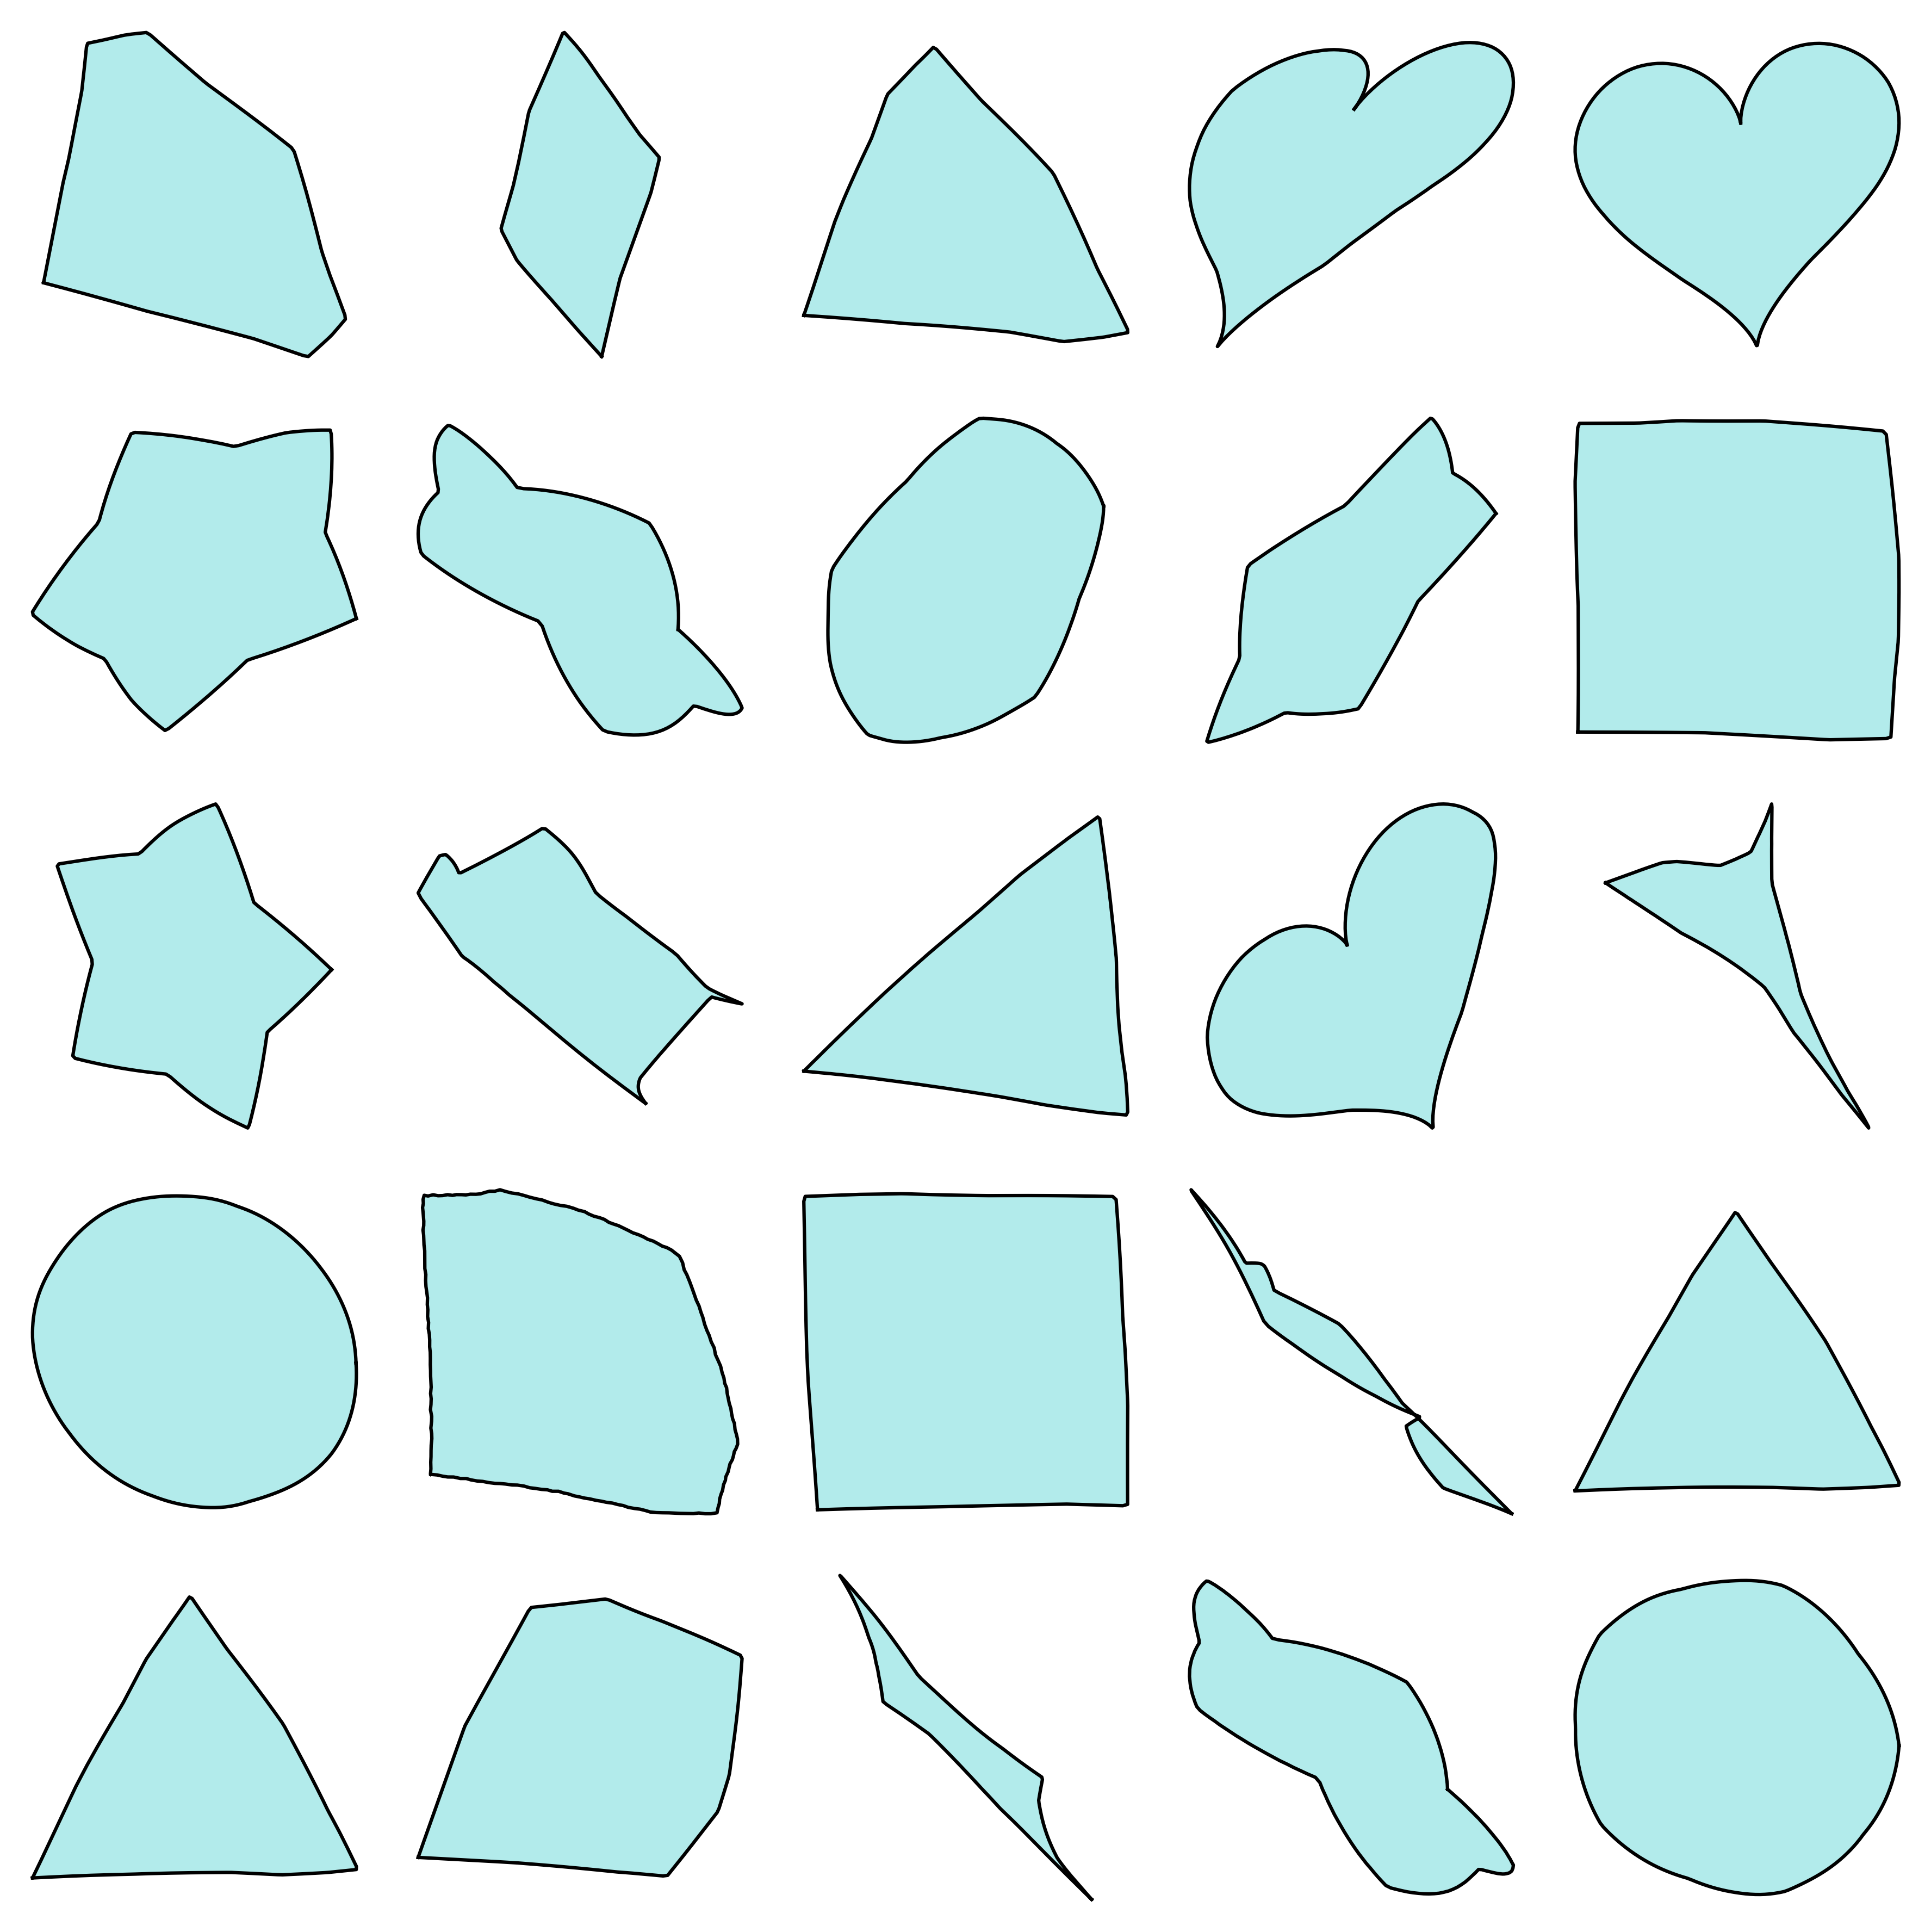
\includegraphics[width=\textwidth]{figures/latent_gen_shapes/GA_11_50_init_pop.png}
        \caption{GA11 Initial Population, VAE Model 1}
        \label{fig:latent_shape_popM1}
    \end{subfigure}
    \hfill
    \begin{subfigure}[b]{0.45\textwidth}
        \centering
        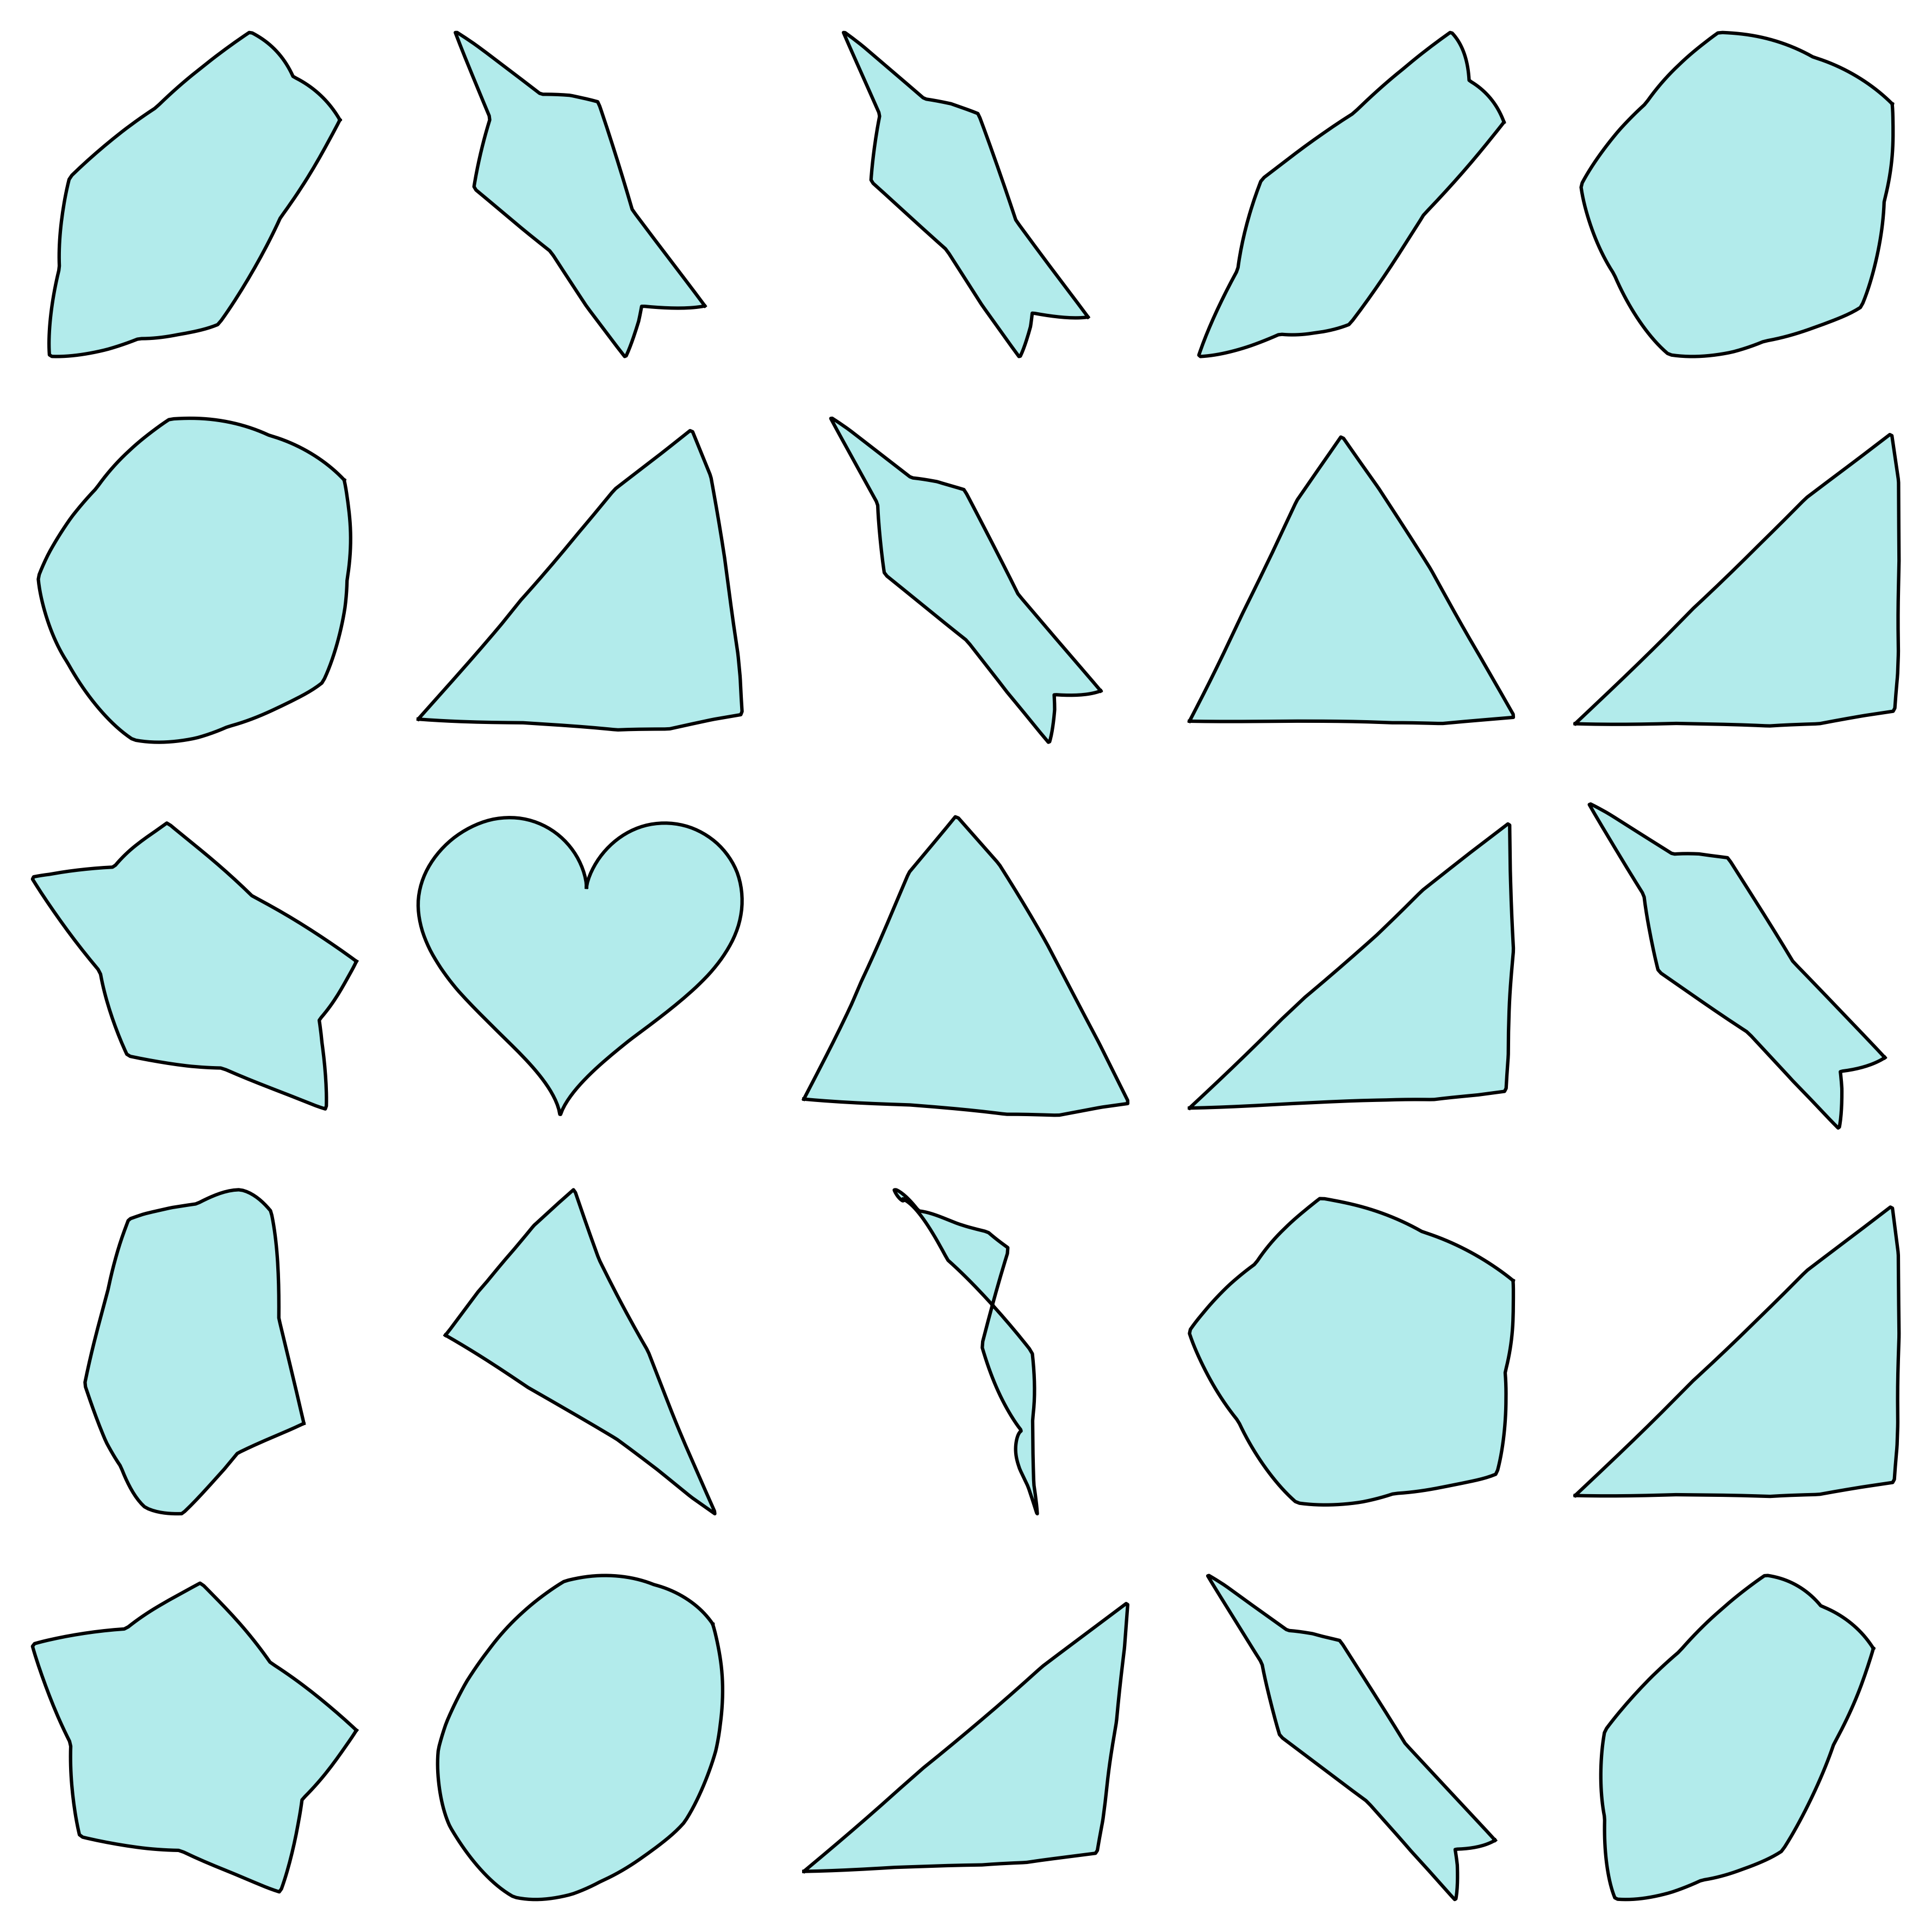
\includegraphics[width=\textwidth]{figures/latent_gen_shapes/GA_15_50initial_pop.png}
        \caption{GA15 Initial Population, Model 4}
        \label{fig:latent_shape_popM4}
    \end{subfigure}
    \caption{Example shapes generated from latent distributions of trained VAEs as initial population for GA.}
    \label{fig:latent_sampled_shapes_GA}
\end{figure}

\begin{table}[h]
\centering
\resizebox{\textwidth}{!}{%
\begin{tabular}{|c|c|c|c|c|c|c|}
\hline
\textbf{GA} & \textbf{Category} & \textbf{Latent Dimensions} & \textbf{Starting Population} & \textbf{Number of Parents} & \textbf{Total Generations} & \textbf{Mutation Probability}  \\
\hline
GA11 & Latent & 2 & 50 & 10 & 100 & 0.05 \\
\hline
GA12 & Latent & 2 & 10 & 3 & 100 & 0.05 \\
\hline
GA13 & Latent & 3 & 50 & 10 & 100 & 0.05 \\
\hline
GA14 & Latent & 3 & 10 & 3 & 100 & 0.05 \\
\hline
GA15 & Latent & 4 & 50 & 10 & 100 & 0.05 \\
\hline
GA16 & Latent & 4 & 10 & 3 & 100 & 0.05 \\
\hline
GA17 & Latent & 5 & 50 & 10 & 100 & 0.05 \\
\hline
GA18 & Latent & 5 & 10 & 3 & 100 & 0.05 \\
\hline
GA19 & Latent & 6 & 50 & 10 & 100 & 0.05 \\
\hline
GA20 & Latent & 6 & 10 & 3 & 100 & 0.05 \\
\hline



\end{tabular}%
}
\caption{Genetic Algorithm Tested Optimisation Tasks for Latent Representations Shapes}
\label{tab:GA_models_latent}
\end{table}


\newpage{}[H]

\section{Results and Discussion}
\subsection{Variational Autoencoder}
The following section will present the results of training the VAE models and provide examples of their generative capability in producing a smooth and continuous continuous latent space. We will present the visualisations of this latent space in combination with the performance surface defined by the compactness metric (see Equation~\eqref{eq:compactness}). While it is trivial to visualise the generated shapes and the resultant performance surface of VAEs with only 2-dimensions, additional dimensions are less easily interpretable. For this reason, we opt to fix all but 2 of the dimensions to z-values of 0 in latent models where the latent dimension is greater than 2. For the highest dimension models, we refrain from presenting all combinations of but instead report on the most informative observations and insightful results from the autoencoder.

\subsubsection{VAE Model 1 - 2D Latent Dimension}

Figure~\ref{fig:model1_loss_plot} shows the loss plot for \textbf{\textit{Model-1}}. The loss reported here is a combination of the mean squared error (MSE) loss, and the Kullback-Leiber divergence shown in Equation~\ref{eq:VAE_loss_function}. A hyperparamater inside the training loss is applied, which we denote $\beta$, a weighting factor for the KL-divergence contribution. We fix $\beta$ to \textbf{1.0}, however, we can vary the influence that the KL-divergence has on the total training loss by increasing or decreasing $\beta$ accordingly. Increasing the $\beta$ value affects the trade-off between reconstruction of the original data, and latent space regularisation, such that larger values will force the model to learn a latent distribution that more closely matches the prior $p(\textbf{z})$, i.e., $\mathcal{N}\sim(0,\textbf{I})$. Setting $\beta$ weighting to would remove the variational component of the VAE. The loss plot the for 2D VAE convergences quickly after ~200 epochs, with an MSE plateauing marginally above 1000. We maintain the same number of epochs for all VAE training routines, since we observe that models quickly.
\begin{figure}[H]
\centering
    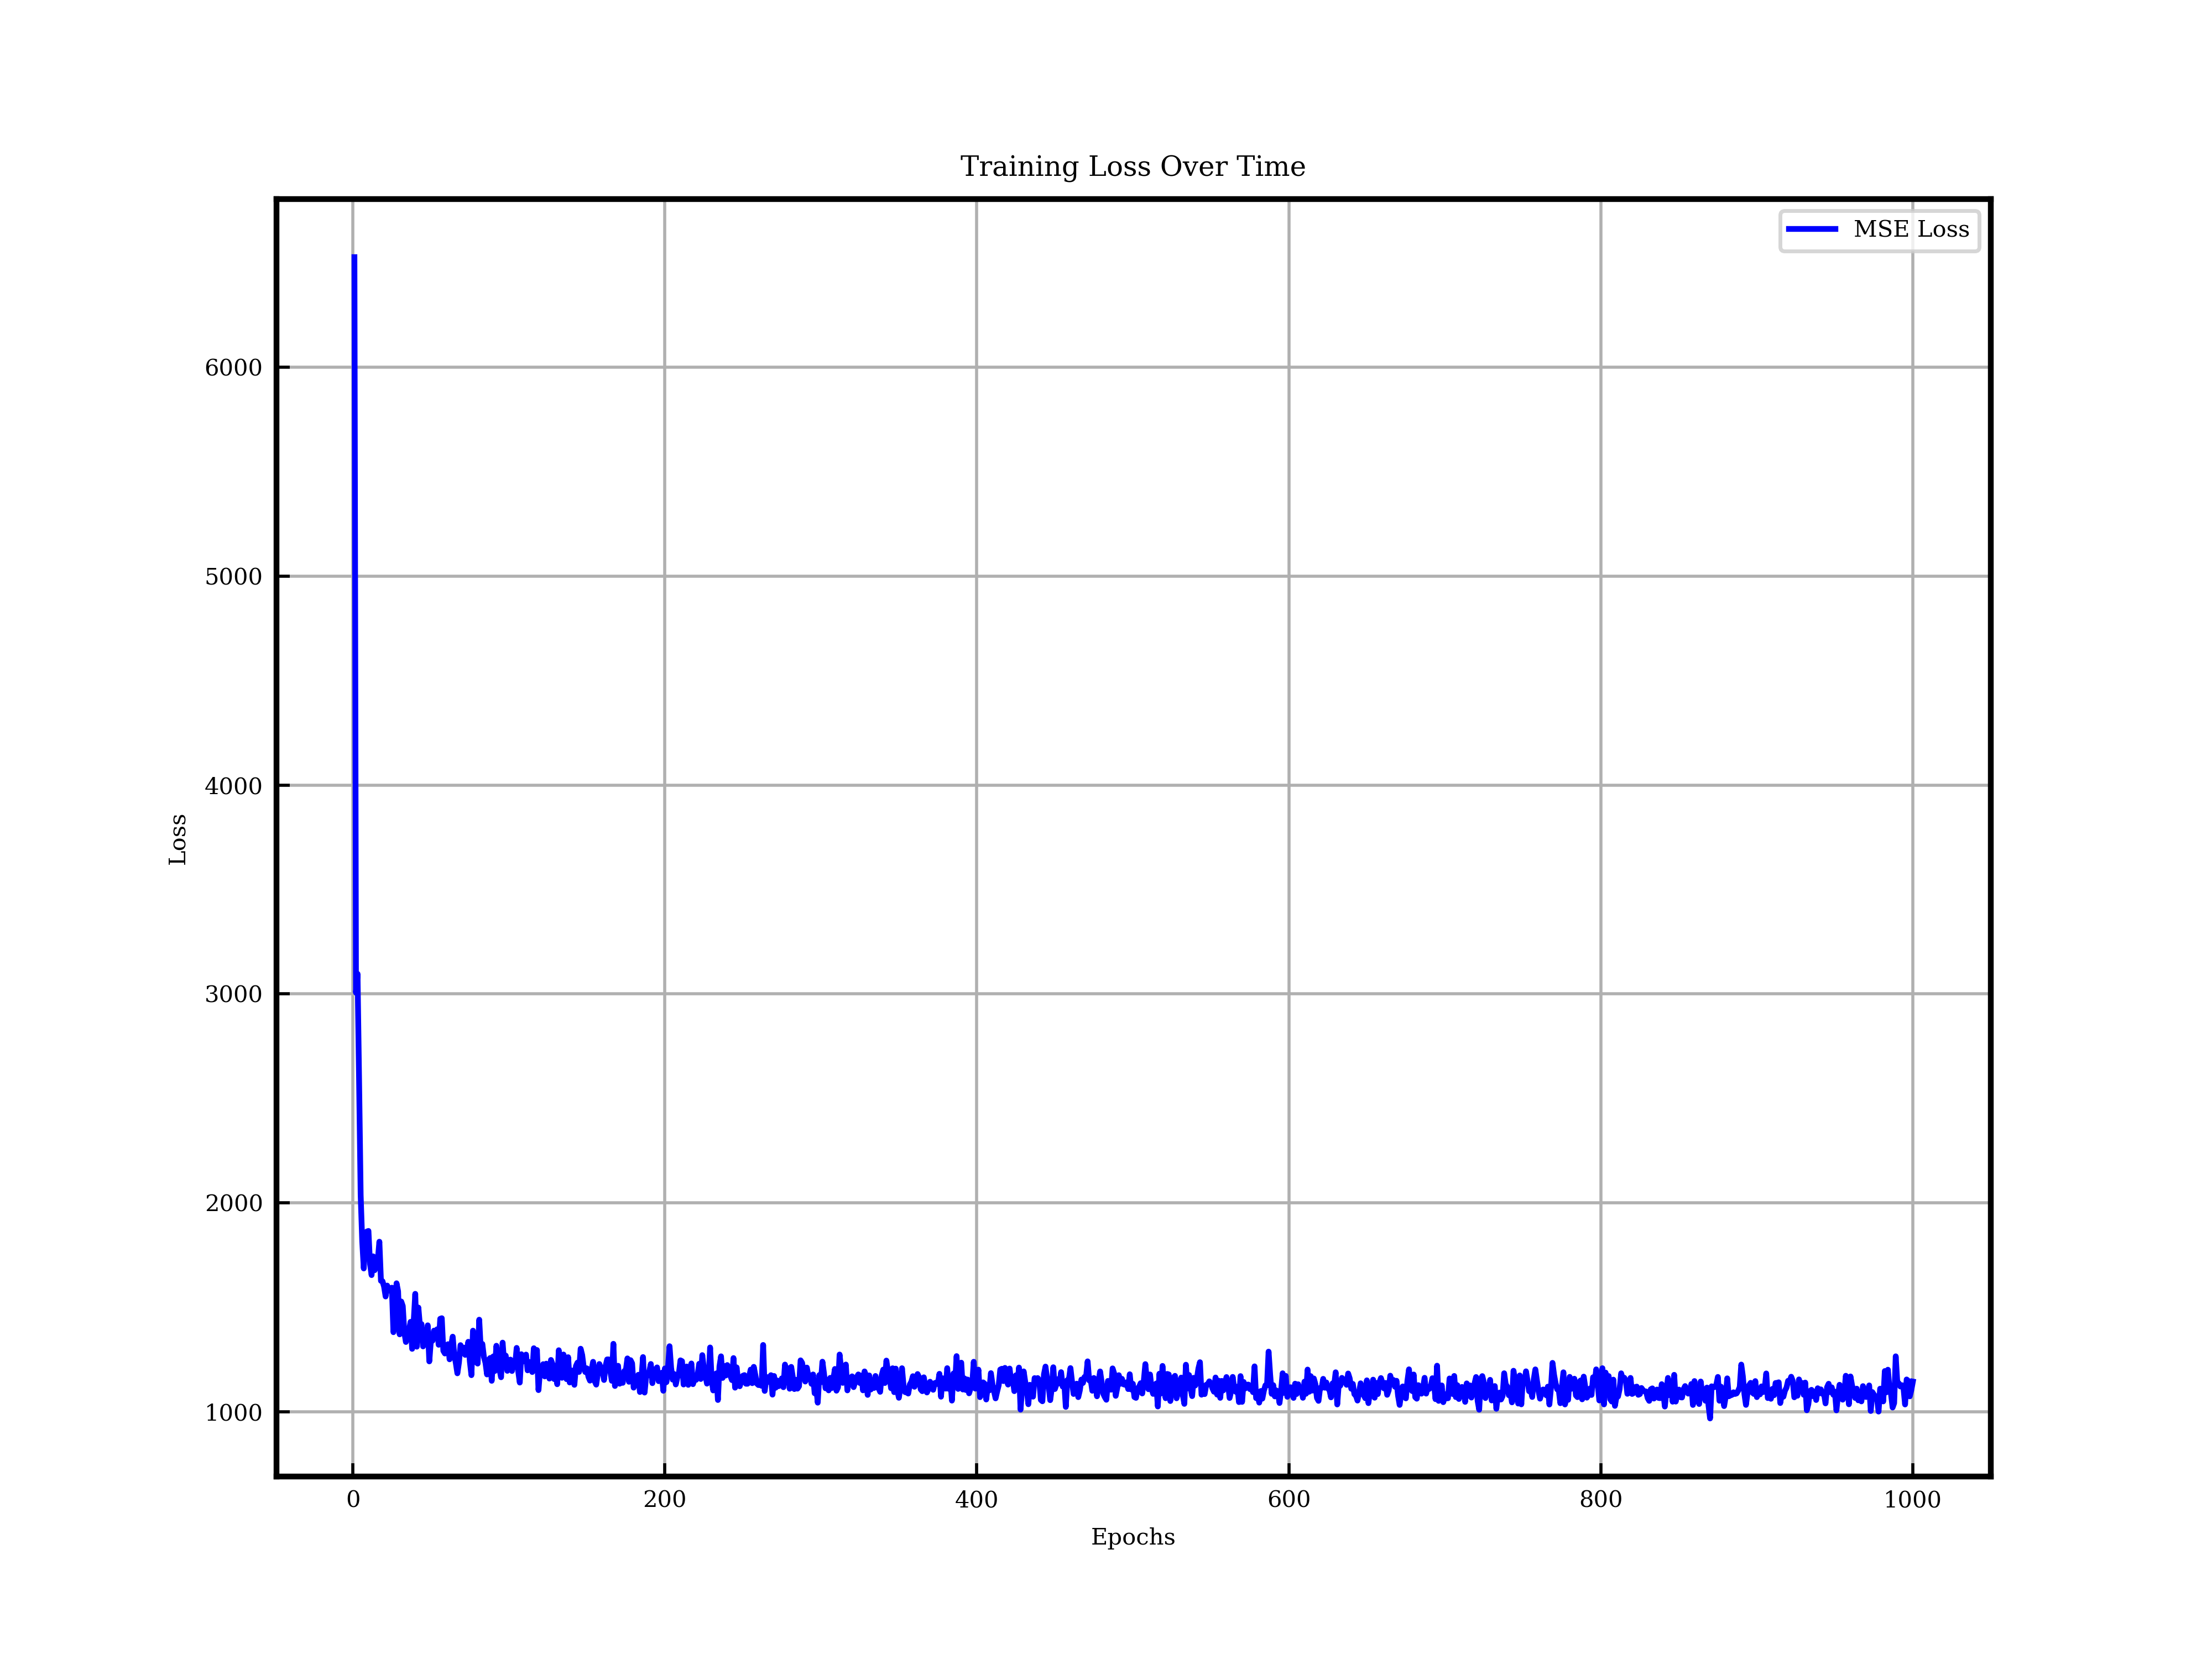
\includegraphics[width=0.75\linewidth]{figures/VAEmodels/model1/loss_plot.png}
    \caption{VAE Model 1 - MSE + KL Loss Plot}
    \label{fig:model1_loss_plot}
\end{figure}
For the purpose of interpreting the associated values of the latent vectors, we proceed to encode all the shapes contained inside the original VAE training dataset via the trained VAE models. Encoding each shape provides a $\mu$ and $\sigma^2$ vector denoting the latent distribution characterising each shape, unlike a determinist auto encoder (or VAE with $\beta=0$). By sampling from each of the latent distributions, we obtain a distribution of latent vectors, where each entry corresponds to a latent value for each latent dimension.  Plotting these distributions in Figure~\ref{fig:model1_latent_dist} reveals the limits of the z-values. It should be considered that  resampling from all the latent distributions associated with the training dataset would reveal a different set of latent values and therefore a different distribution, though for large enough samples, these should tend towards the mean. We assume that that the limits of the distributions do not vary considerably. By interrogating these distributions, we apply bounds to the latent values for which to sample from in order to generate new shapes. Be specifying bounds of the z-values based on upon those observed via encoding of the original VAE training data, we confine our generation of new shapes within this range for the purpose of visualisation and to generate a population for optimisation workflows. Figure~\ref{fig:model1_latent_dist} shows the distribution of all latent values obtained by encoding all shapes in the training dataset.
\begin{figure}[H]
    \centering
    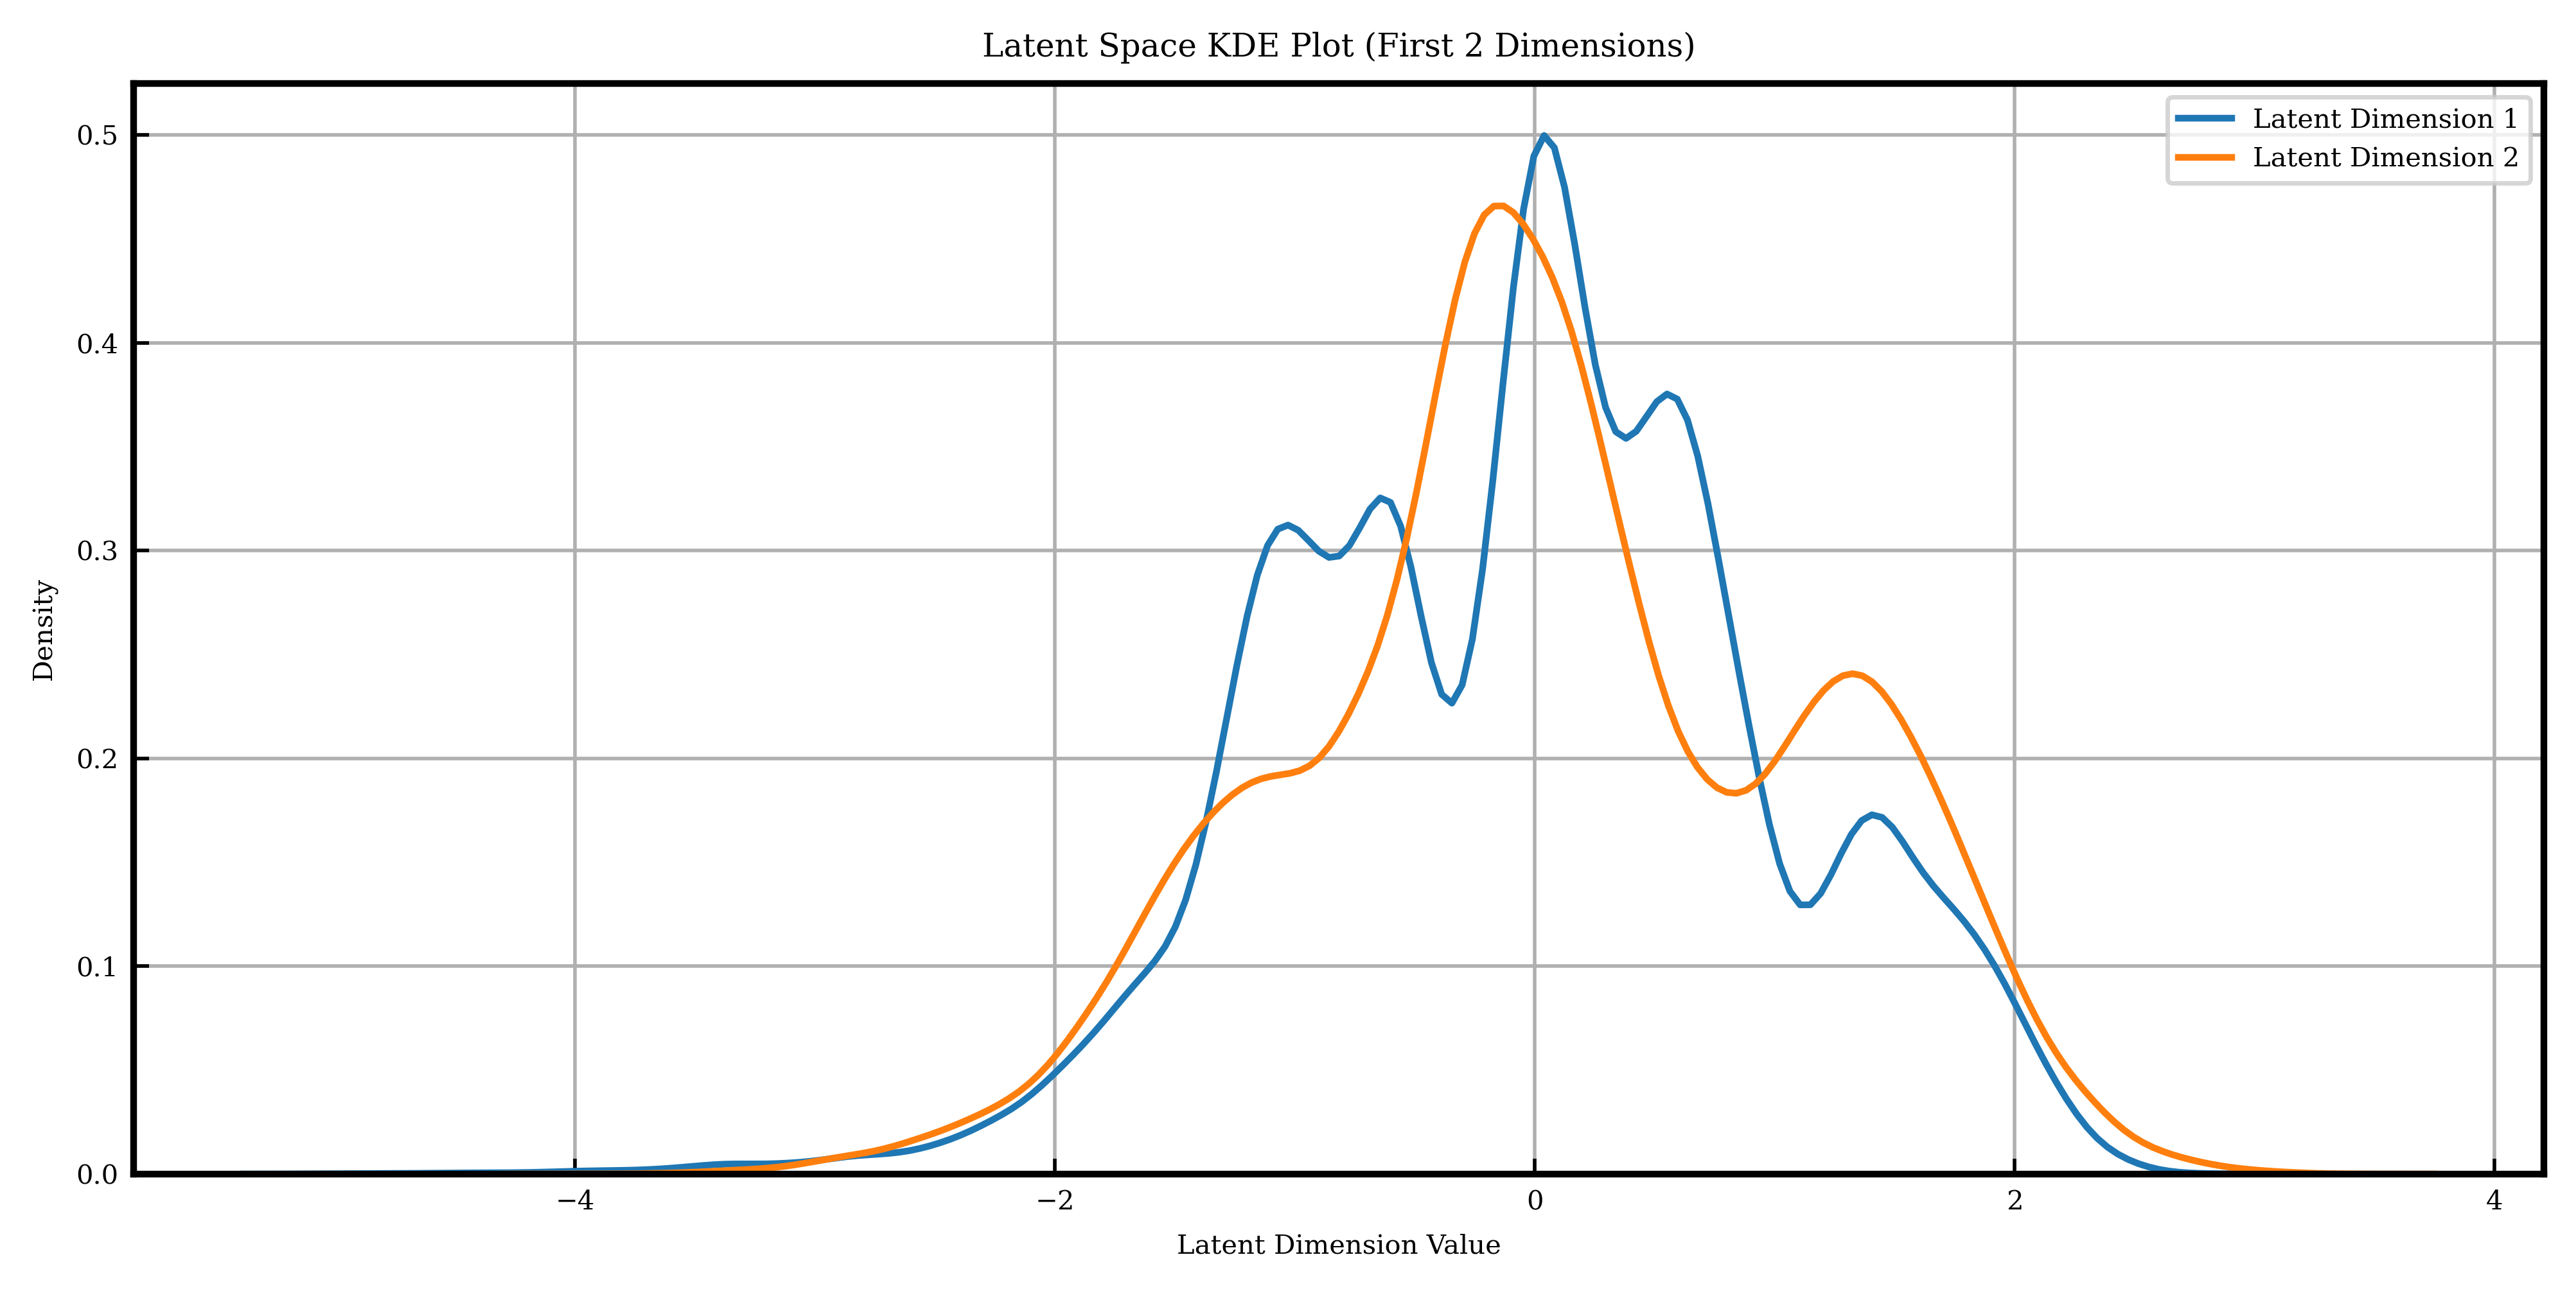
\includegraphics[width=0.75\linewidth]{figures/VAEmodels/model1/latent_distribution.png}
    \caption{Model 1 - Latent dimension distributions over all training data}
    \label{fig:model1_latent_dist}
\end{figure}

Despite the latent distribution showing limits ~[-4,+4] for both latent dimensions we select [-3,+3] for visualisation of the shapes generated over the latent space, this is to increase confidence that we are within the distribution of the training data. We sample 50 latent values between [-3,+3] for each latent dimension maintain this resolution of interrogation points for all VAE models herein. The shapes shown in Figure~\ref{fig:model1_latent_visualisation} are generated by decoding the latent values at each coordinate in the 50x50 grid $(Z_1,Z_2)$. The resultant shapes are also evaluated according to the compactness metric (Equation~\eqref{eq:compactness}), with the compactness metric overlaid as a colour map to demonstrate the performance surface. The performance surface generated is complex, with numerous local minima. Values for compactness across the two latent dimensions have a max 3.0 and minimum of 1.2. The original shapes provided as training data to the VAE can also be recognised in Figure~\ref{fig:model1_latent_visualisation}, with hearts triangles, squares emerging.

\begin{figure}[H]
    \centering
    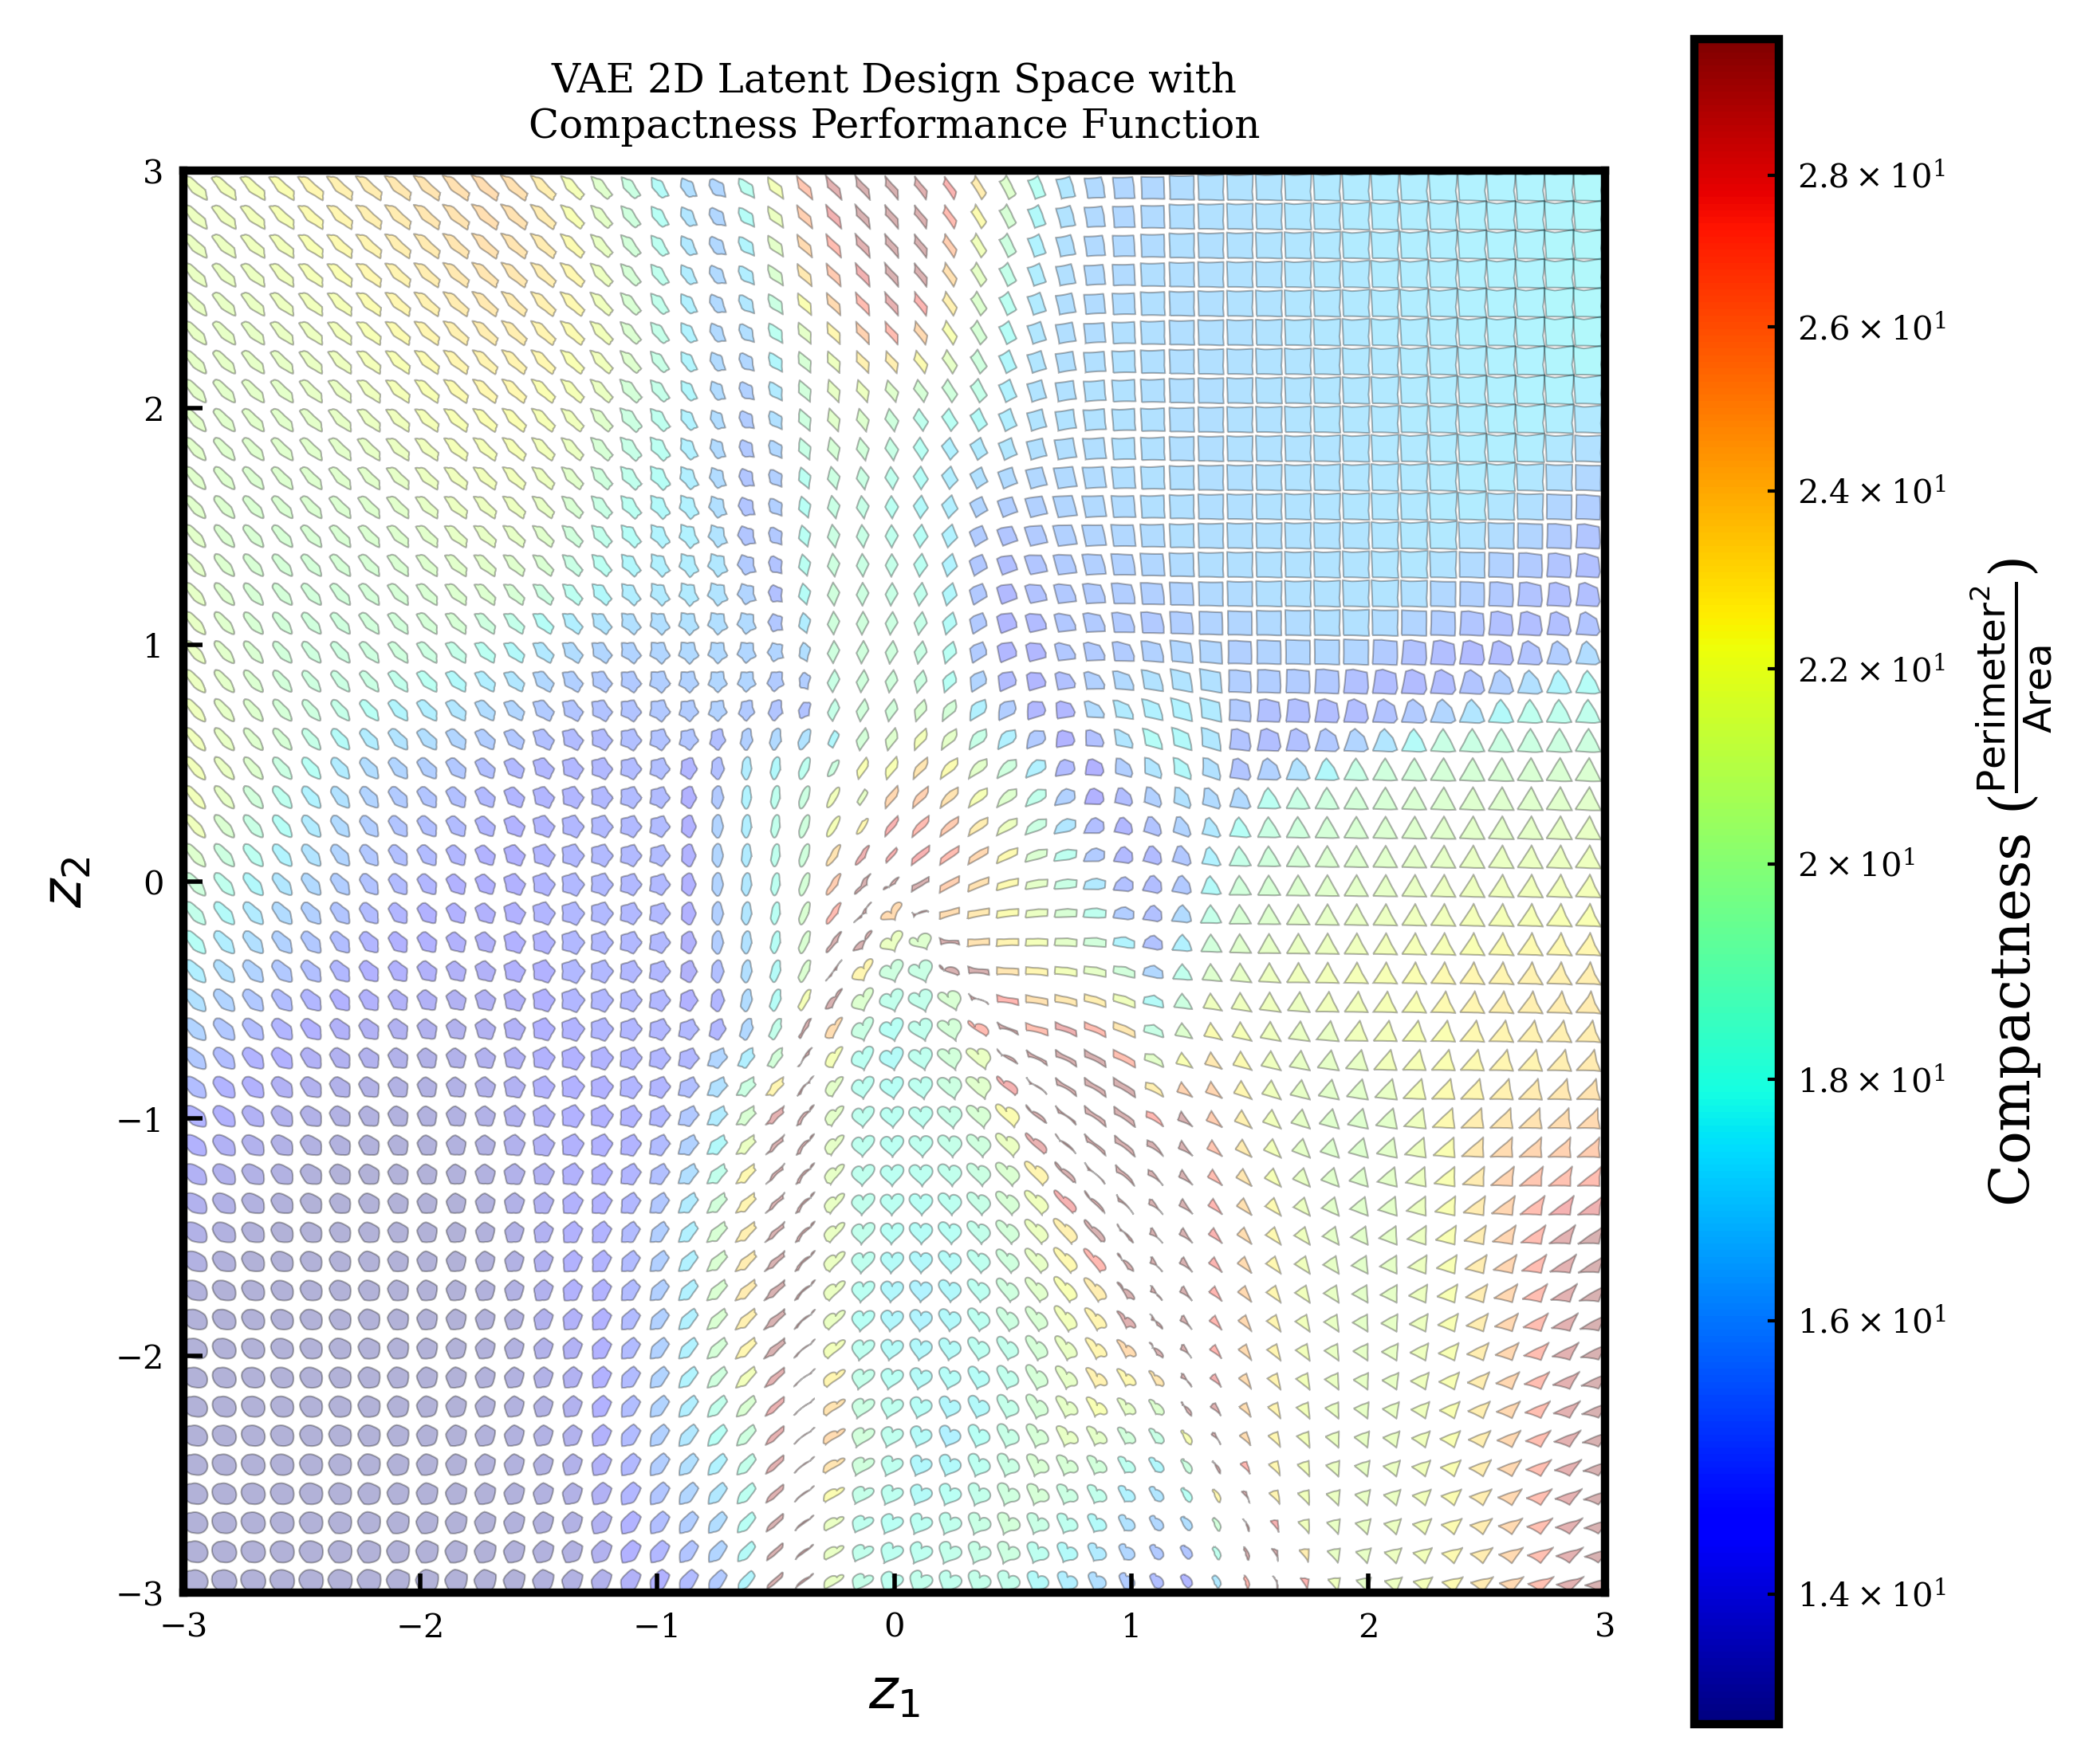
\includegraphics[width=0.75\linewidth]{figures/VAEmodels/model1/latent_vis_1000epochs.png}
    \caption{Model 1 - Latent dimension 1 \& 2 with compactness colormap.}
    \label{fig:model1_latent_visualisation}
\end{figure}

\subsubsection{VAE Model 2 - 3D Latent Dimension}
VAE model 2, employing a third dimension in the latent vector, demonstrates similar learning error with a loss curve that plateaus around MSE of 1000 in less than 100 epochs, when trained with a learning rate of $1\times10^{-4}$ and batch size of 512. The latent distribution plot is shown in Figure~\ref{fig:model2_latent_dist}. The distributions reveal similar minimum and maximum values for the latent values of each dimension, centralised around 0. The third latent dimension demonstrates multi-modality, with peaks seen ~1.5 and at 0 and ~0.5, whereas latent dimension 1 and 2 more closely reflect a standard normal distribution.


\begin{figure}[H]
\centering
    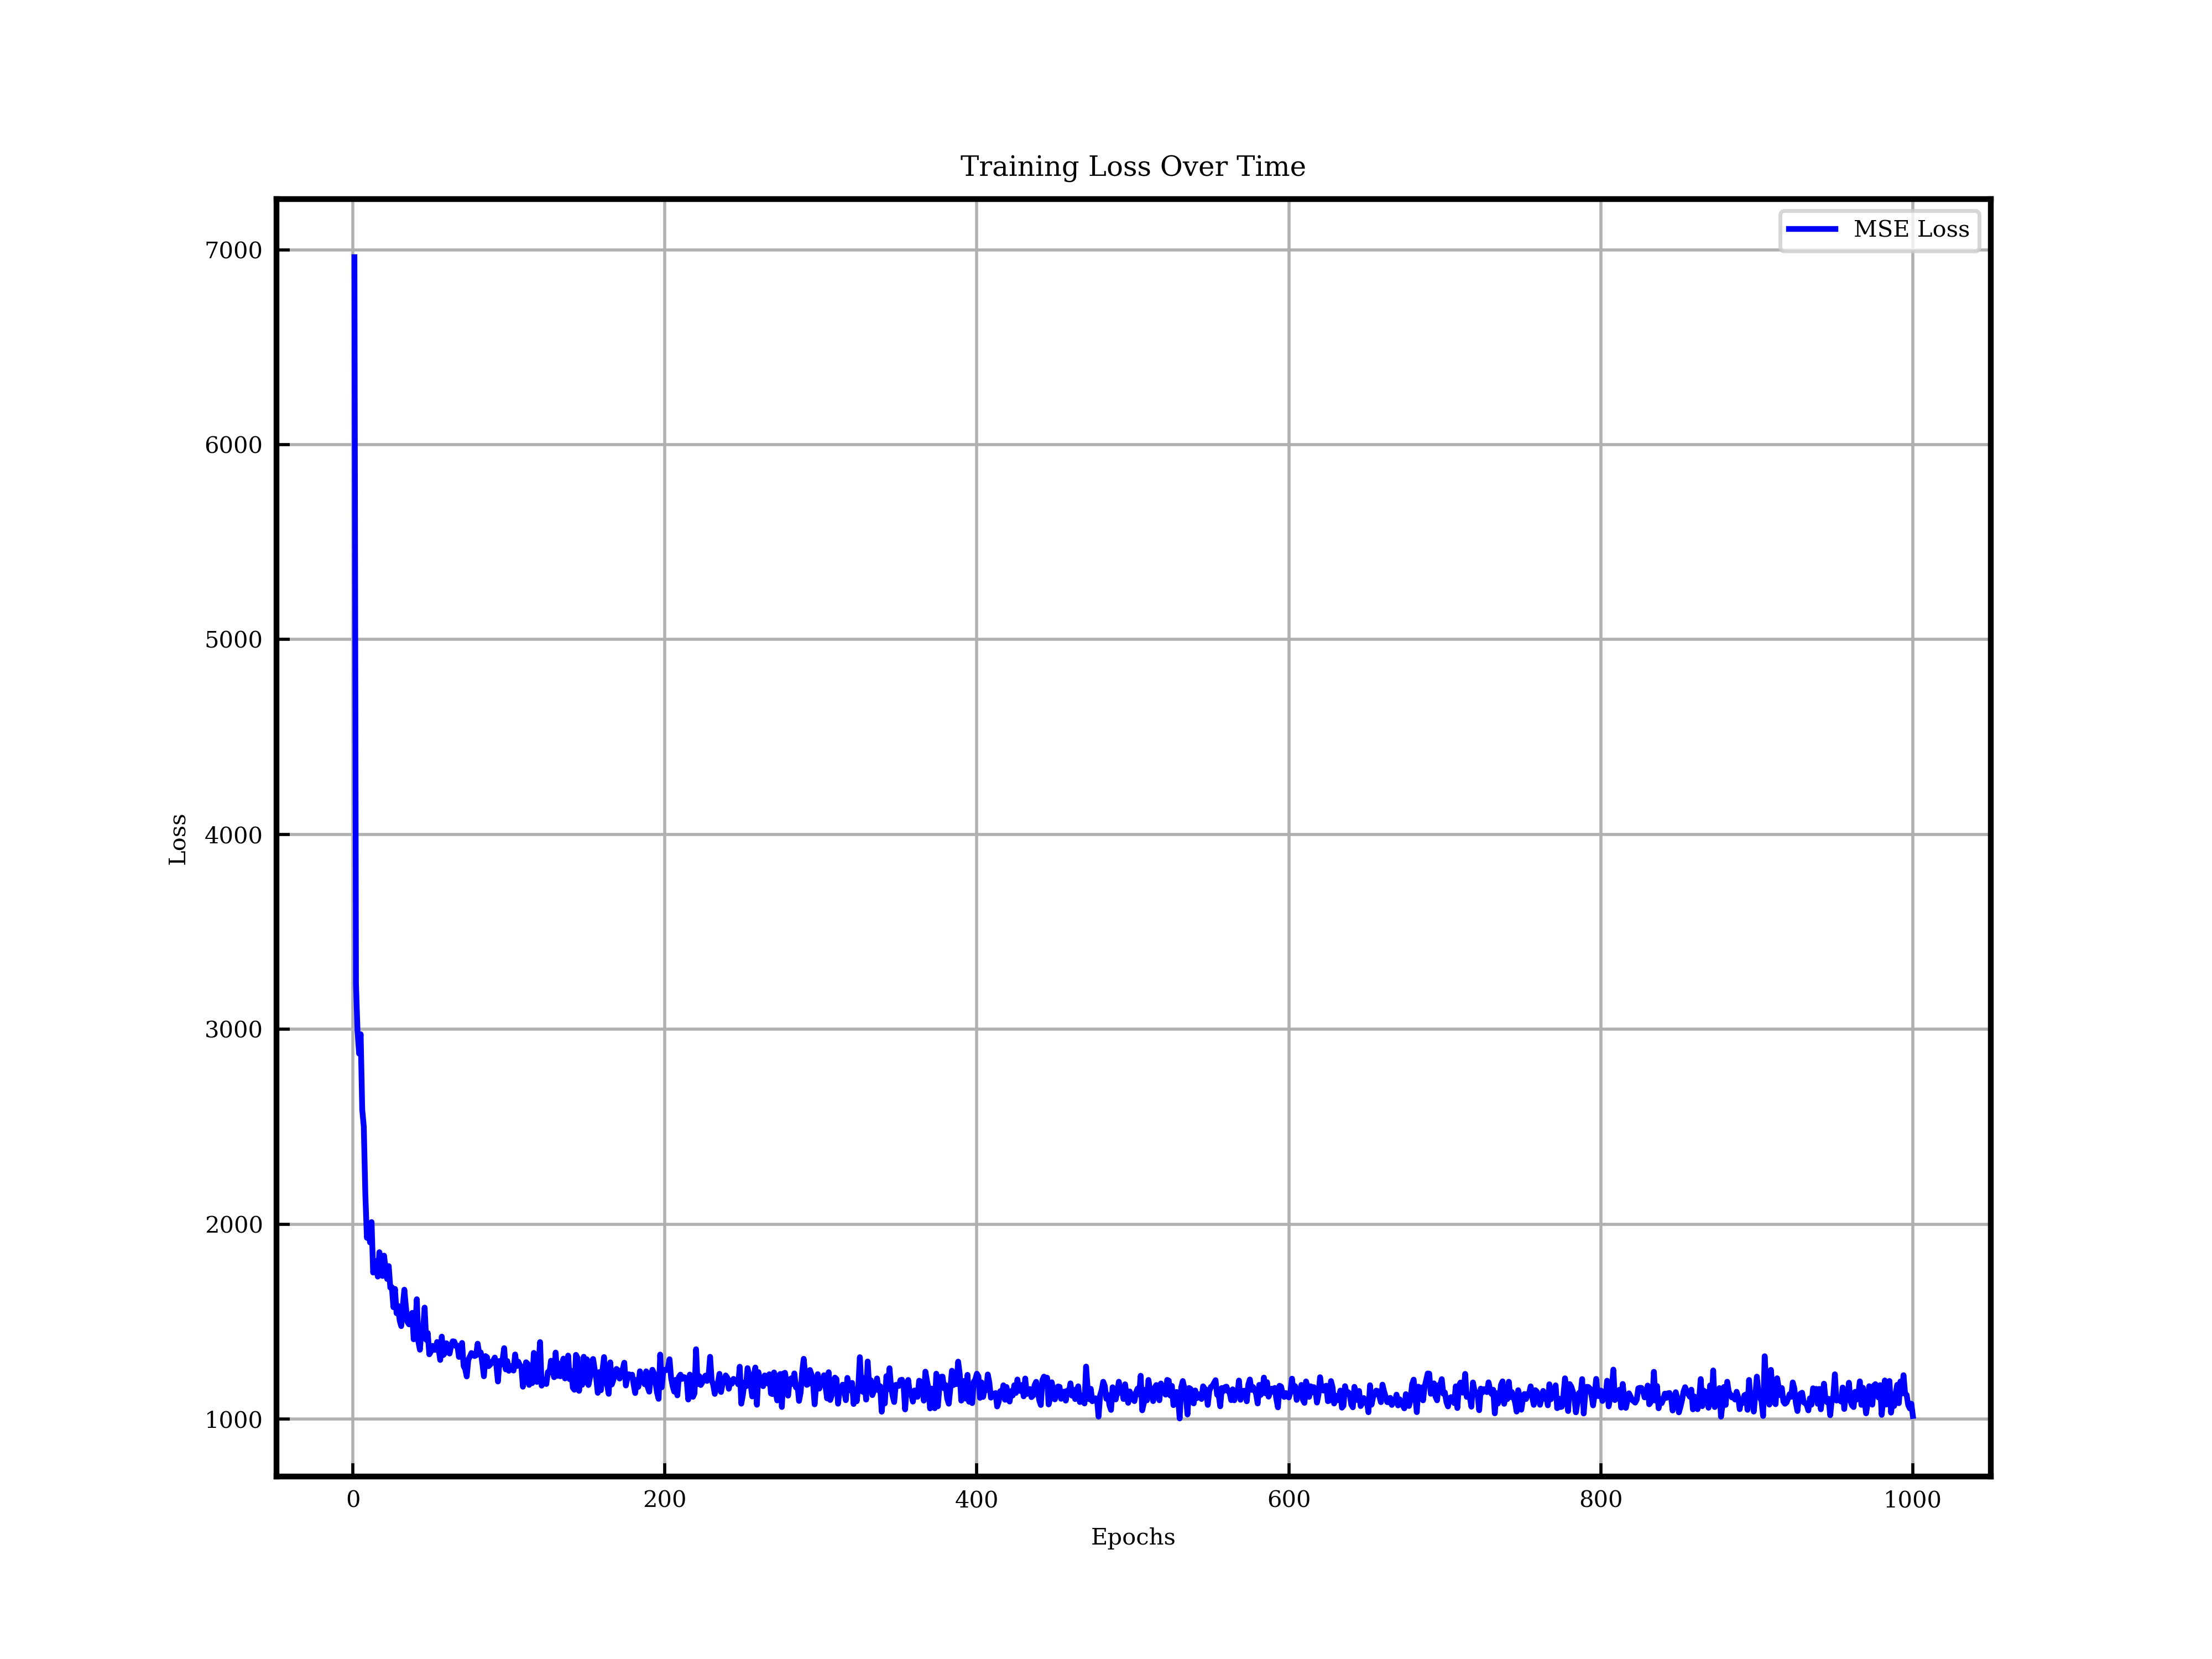
\includegraphics[width=0.75\linewidth]{figures/VAEmodels/model2/loss_plot.png}
    \caption{VAE Model 2 - MSE + KL Loss Plot}
    \label{fig:model2_loss_plot}
\end{figure}

\begin{figure}[H]
    \centering
    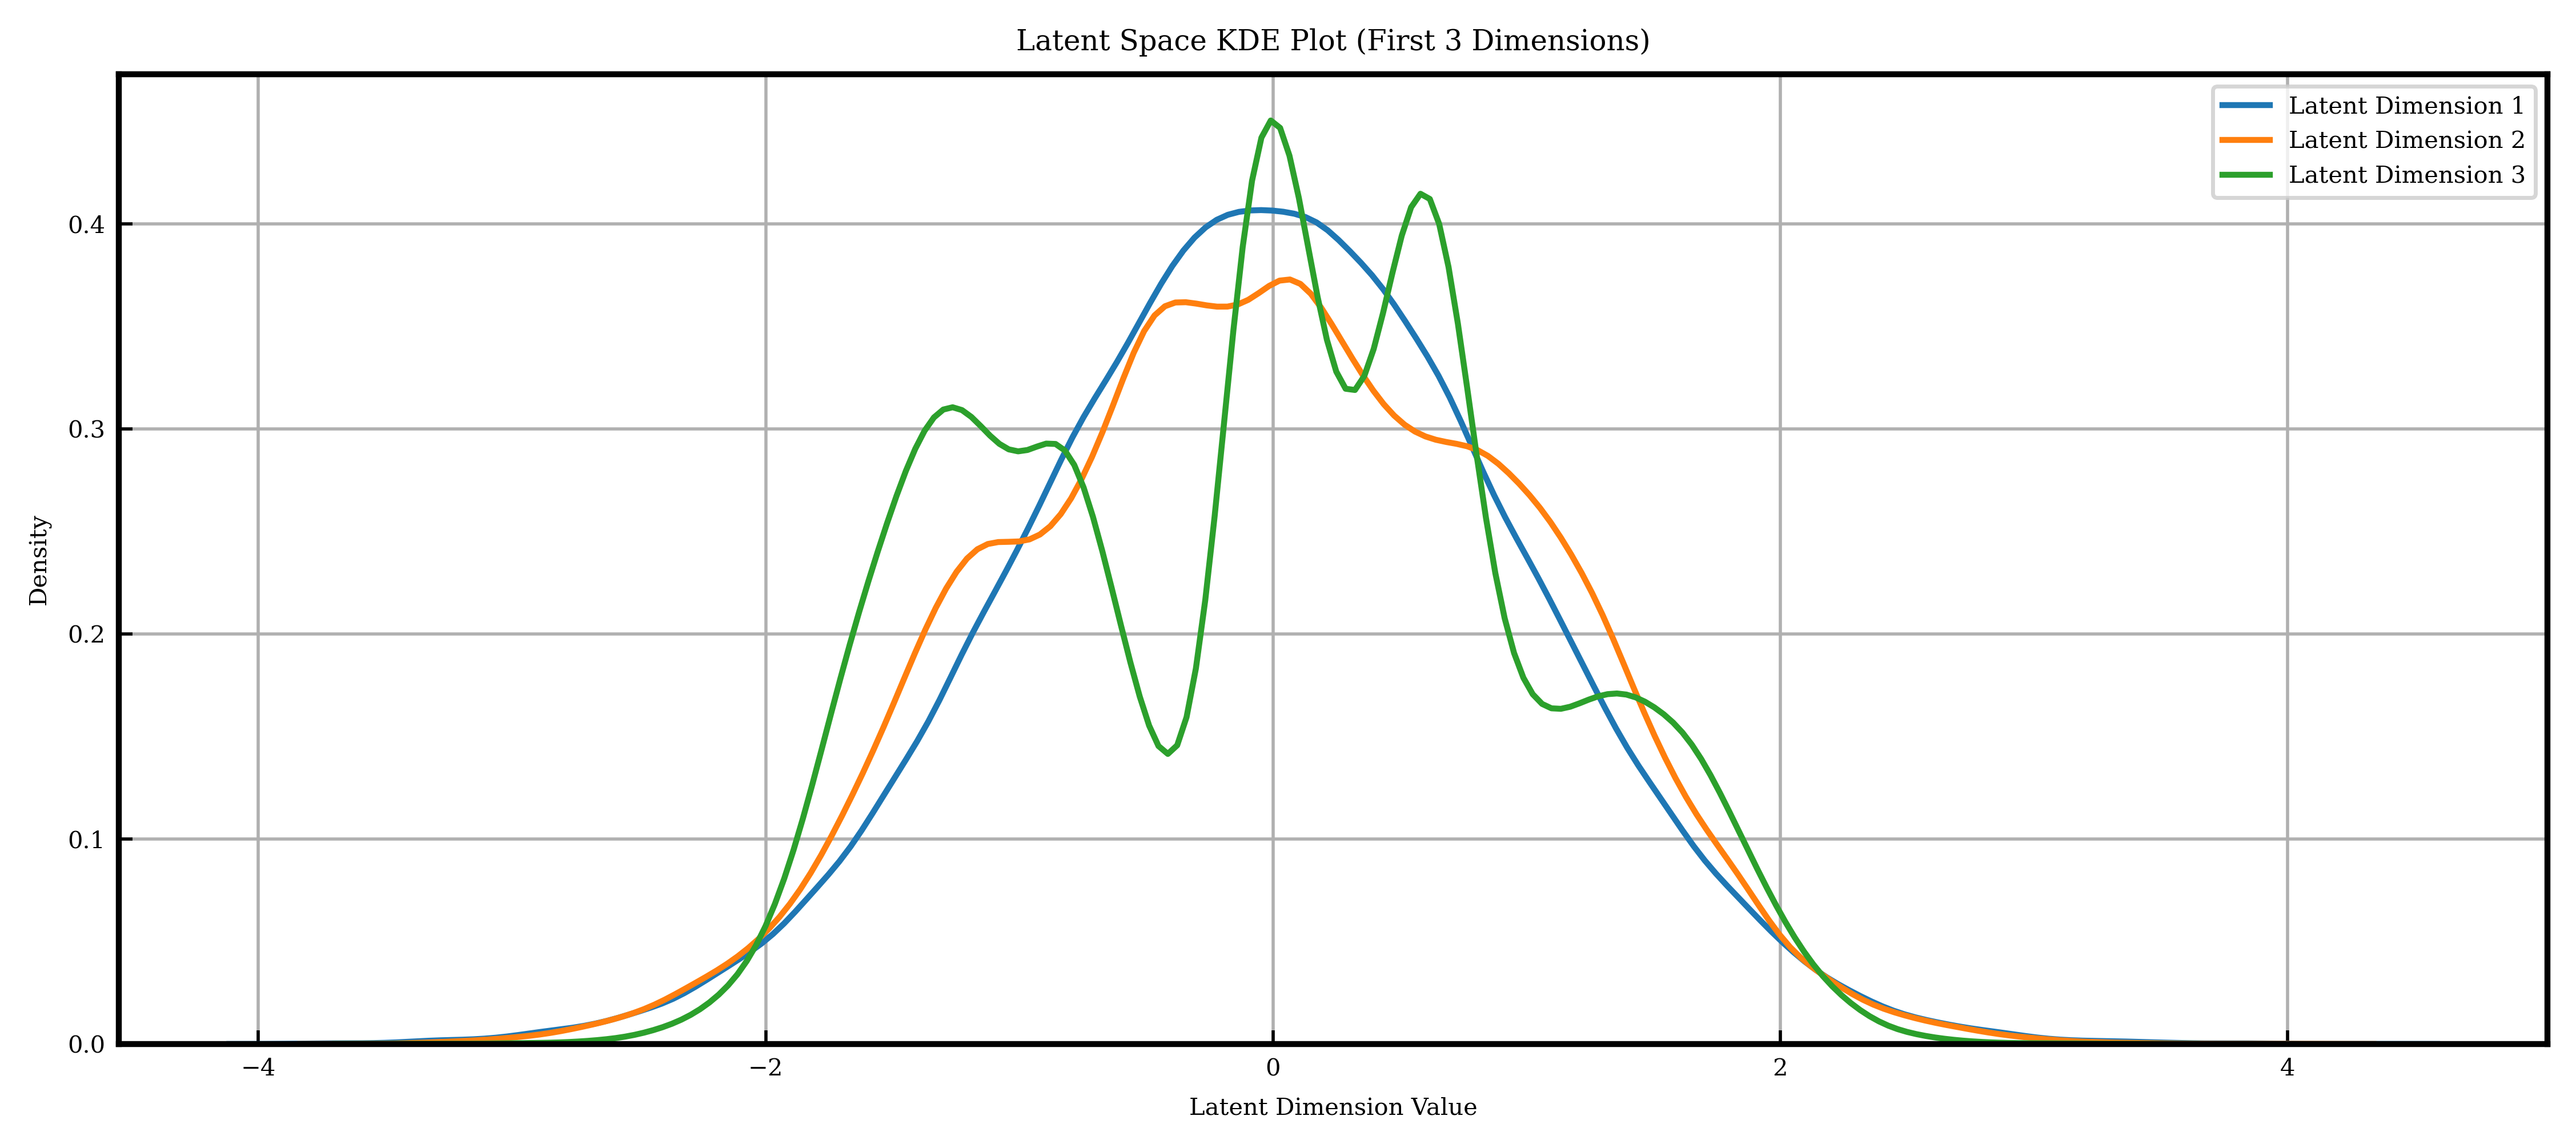
\includegraphics[width=0.75\linewidth]{figures/VAEmodels/model2/latent_distribution.png}
    \caption{Model 2 - Latent dimension distributions over all training data}
    \label{fig:model2_latent_dist}
\end{figure}

To visualise the resultant generated shapes, we present visualisations over 2 latent dimensions, while fixing the third, as shown in Figure~\ref{fig:model2_latent_vis}. All latent dimension values except for those shown on the axis of the visualisations are fixed at $0.0$. For the 3D VAE, this results in 3 possible combinations of latent visualisations in 2D. Only Figure~\ref{fig:model2_fixz1_latent} demonstrates significant variation of the generated shapes when traversing the $Z_1$ and $Z_2$ latent dimensions, with a performance surface observed similar to that seen with the 2D latent model in Figure~\ref{fig:model1_latent_visualisation}. The latent surfaces shown in \ref{fig:model2_fixz2_latent} and \ref{fig:model2_fixz3_latent} only demonstrate variation of the generated shapes when moving in the $Z_3$ and $Z_2$ dimensions respectively, this is also reflected in a non-varying change in the colormap denoting no change in the compactness values when changing these z-values, when the 3rd latent value is fixed at 0. For Figure~\ref{fig:model2_fixz3_latent}, $Z_2$ values below appear to generate only variations of hearts, with no major variation in the compactness value for varying. Only hearts, diamonds and variations of a parallelogram are evident when $Z_3$ is fixed, whereas when fixing $Z_2$ a greater diversity of shapes are generated over latent values between [-3,+3] including triangles, stars, pentagons despite demonstrating banding across all values of $Z_1$. There are no signs of discontinuities in the performance surface, revealing a smooth and continuous latent space which reflects in the smoothness of the evaluated compactness values.

\begin{figure}[H]
  \centering
  \begin{subfigure}{0.8\textwidth}
  \centering
    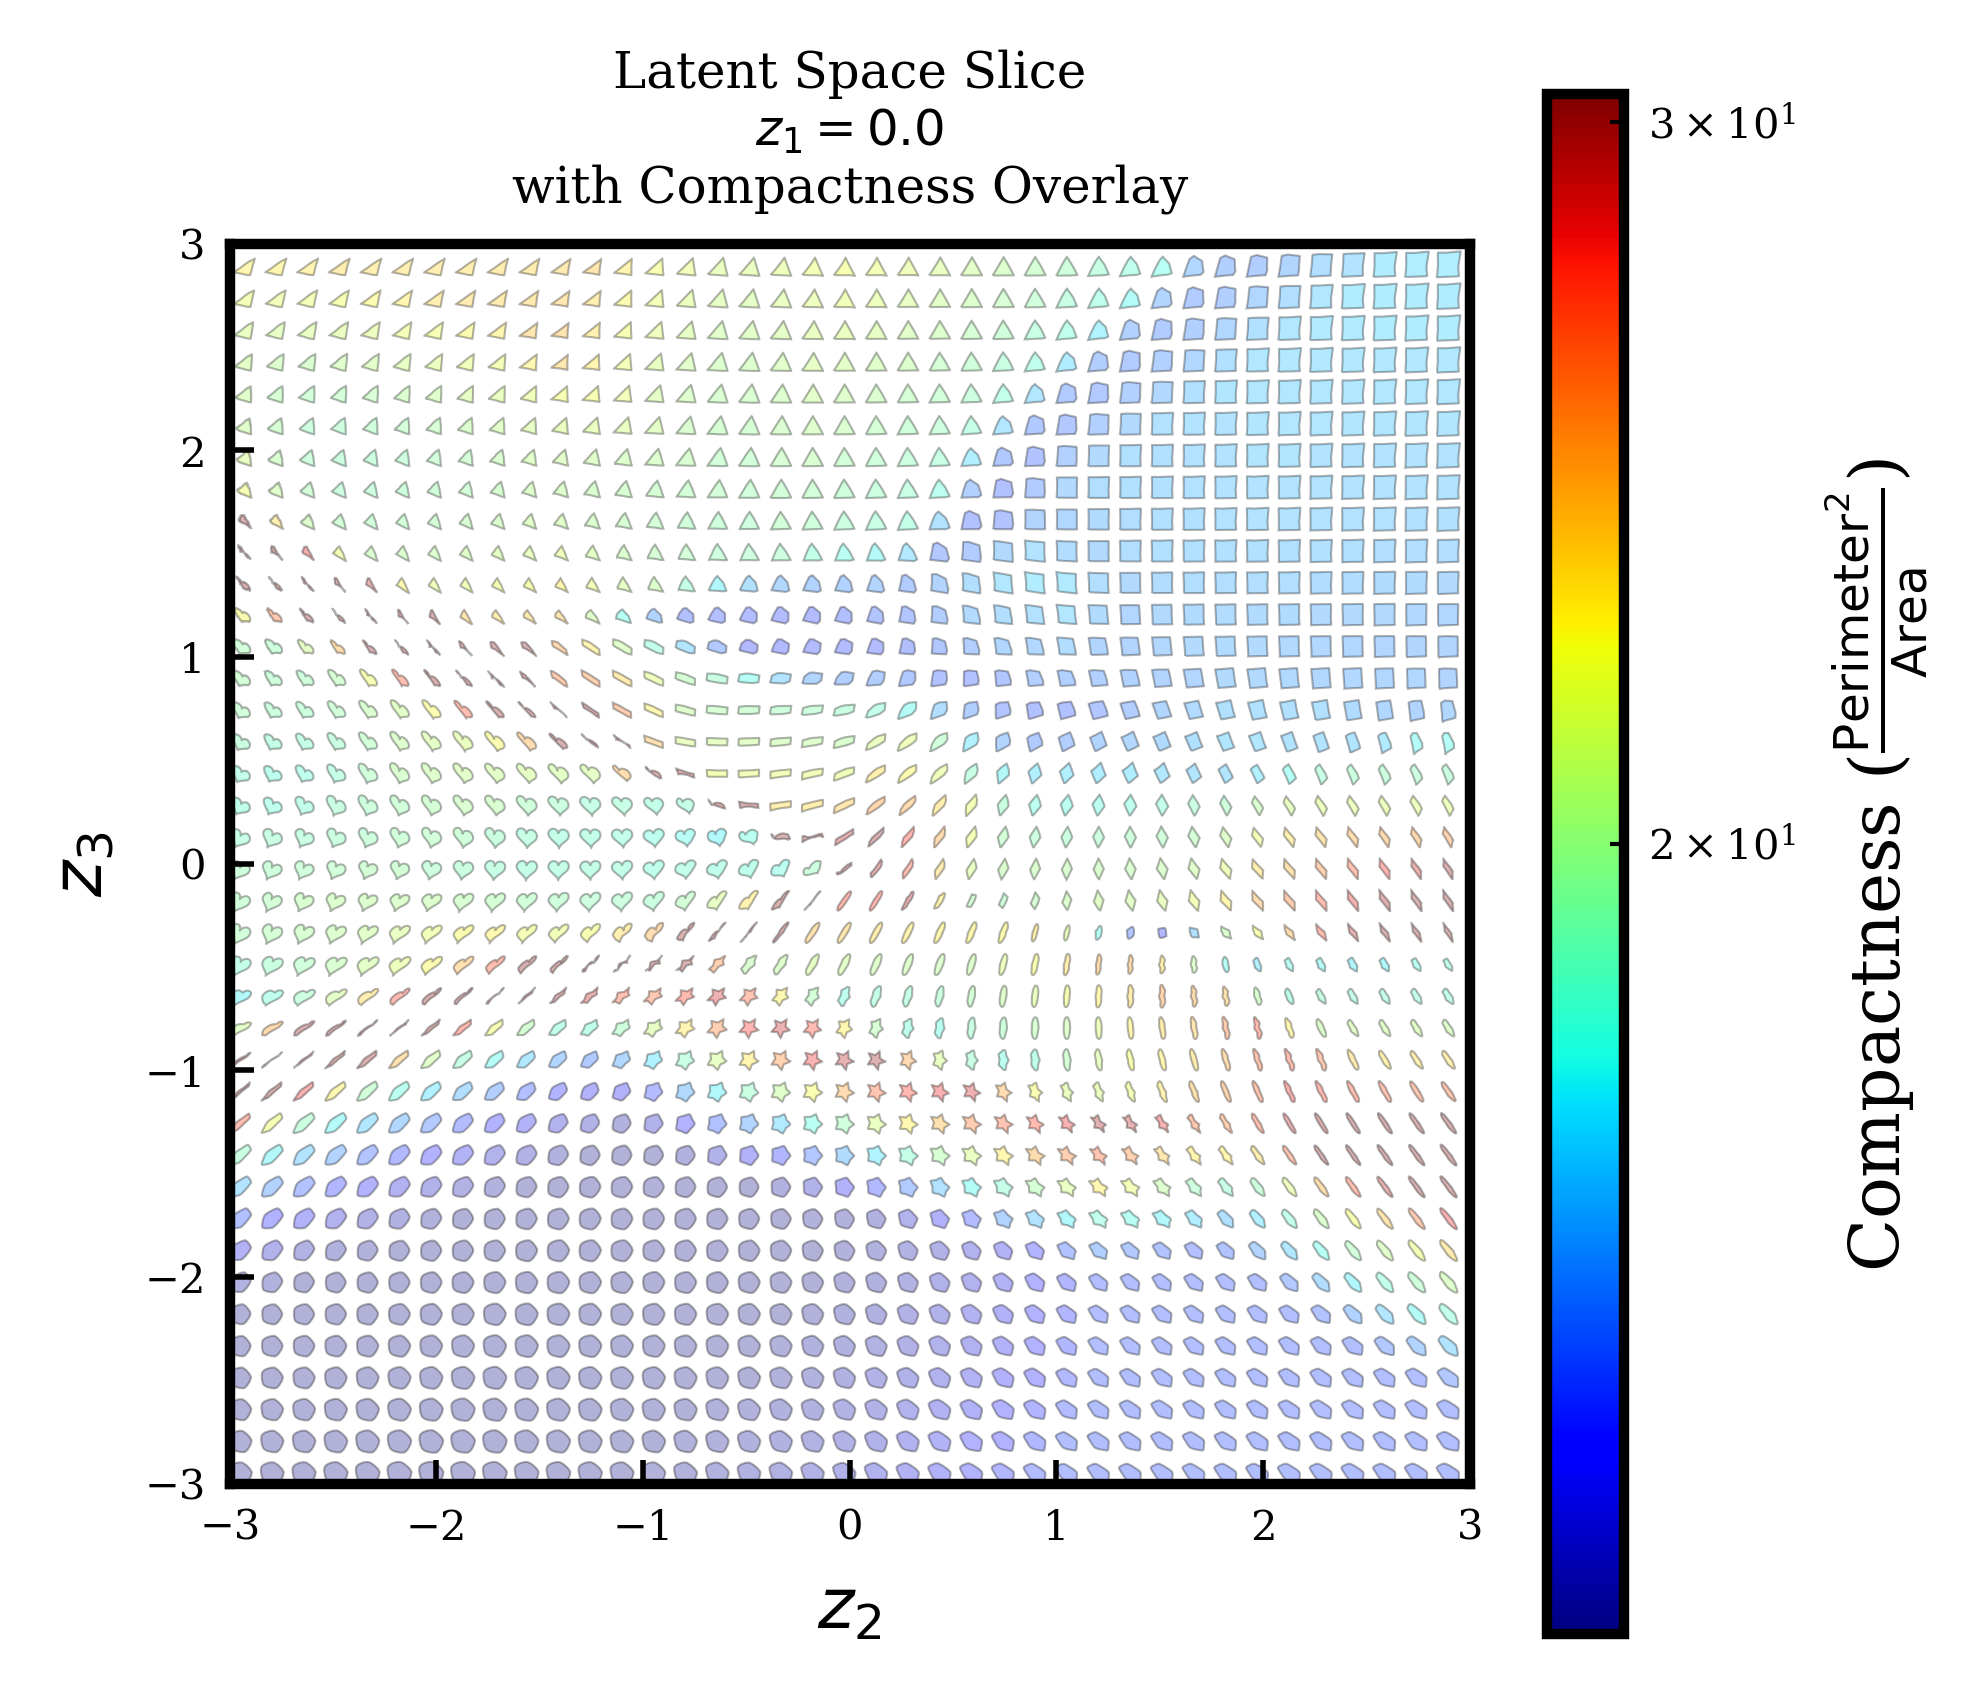
\includegraphics[height=0.3\textheight]{figures/VAEmodels/model2/fix_z1_0.0.png}
    \caption{$Z_1=0.0$}
    \label{fig:model2_fixz1_latent}
  \end{subfigure}
  \par\medskip
  \begin{subfigure}{0.8\textwidth}
  \centering
    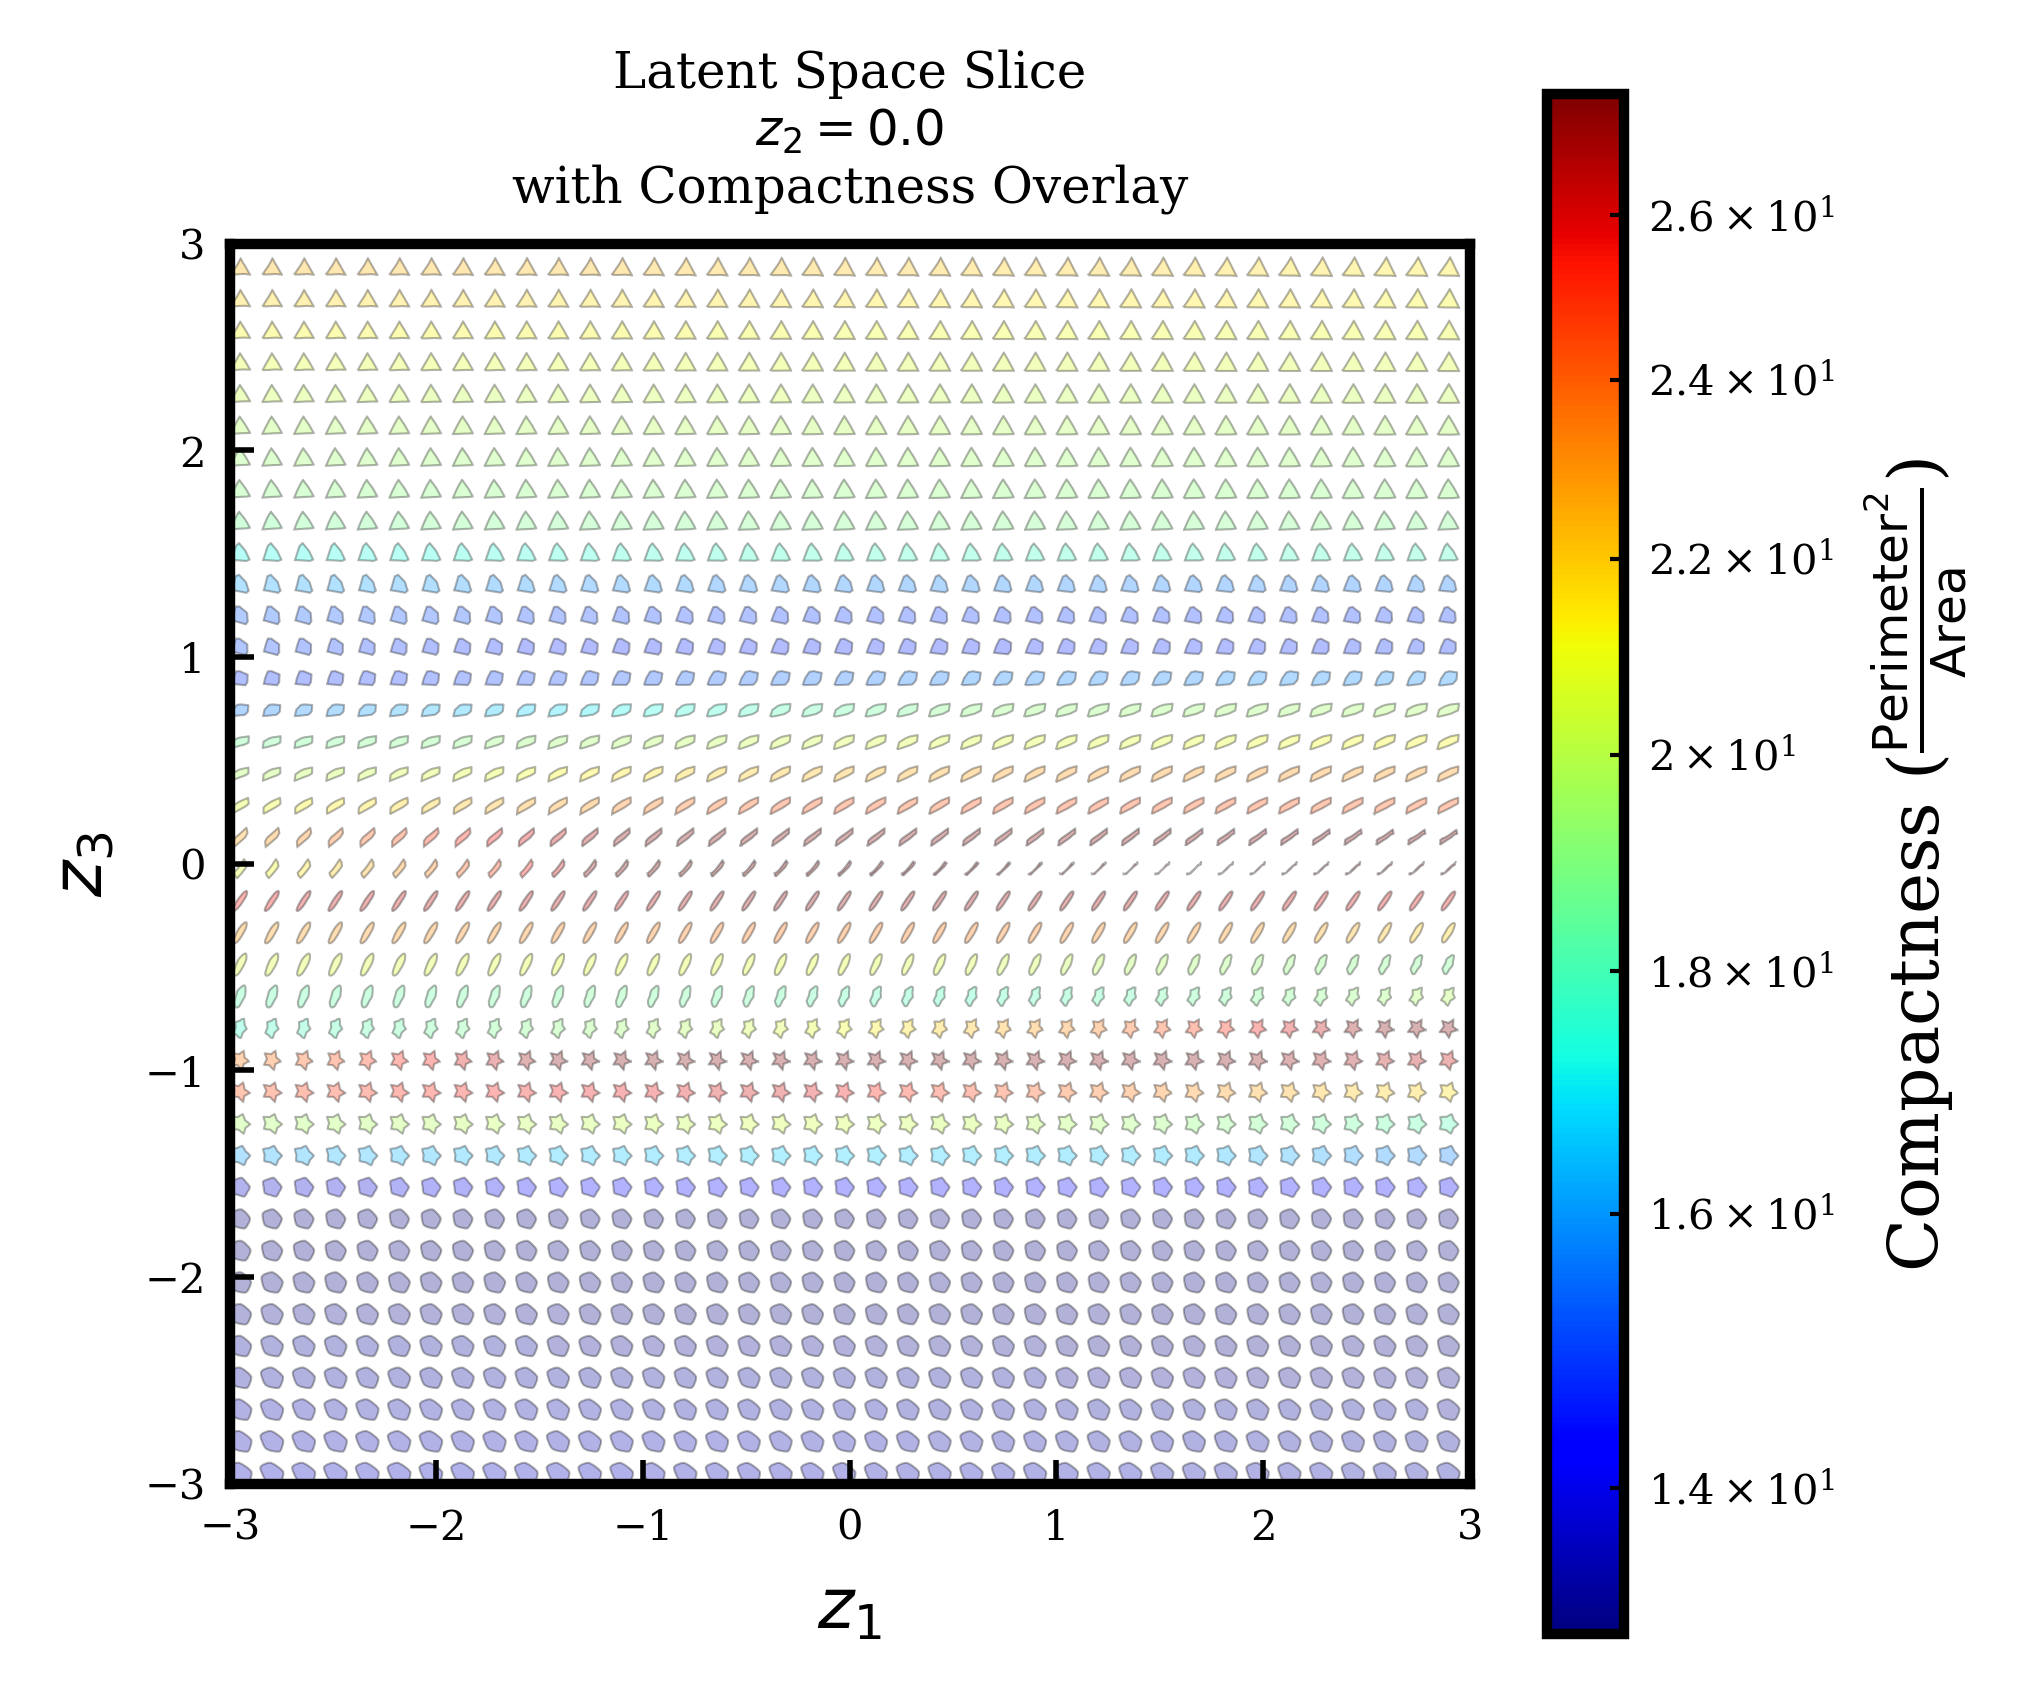
\includegraphics[height=0.3\textheight]{figures/VAEmodels/model2/fix_z2_0.0.png}
    \caption{$Z_2=0.0$}
    \label{fig:model2_fixz2_latent}
  \end{subfigure}
  \par\medskip
  \begin{subfigure}{0.8\textwidth}
  \centering
    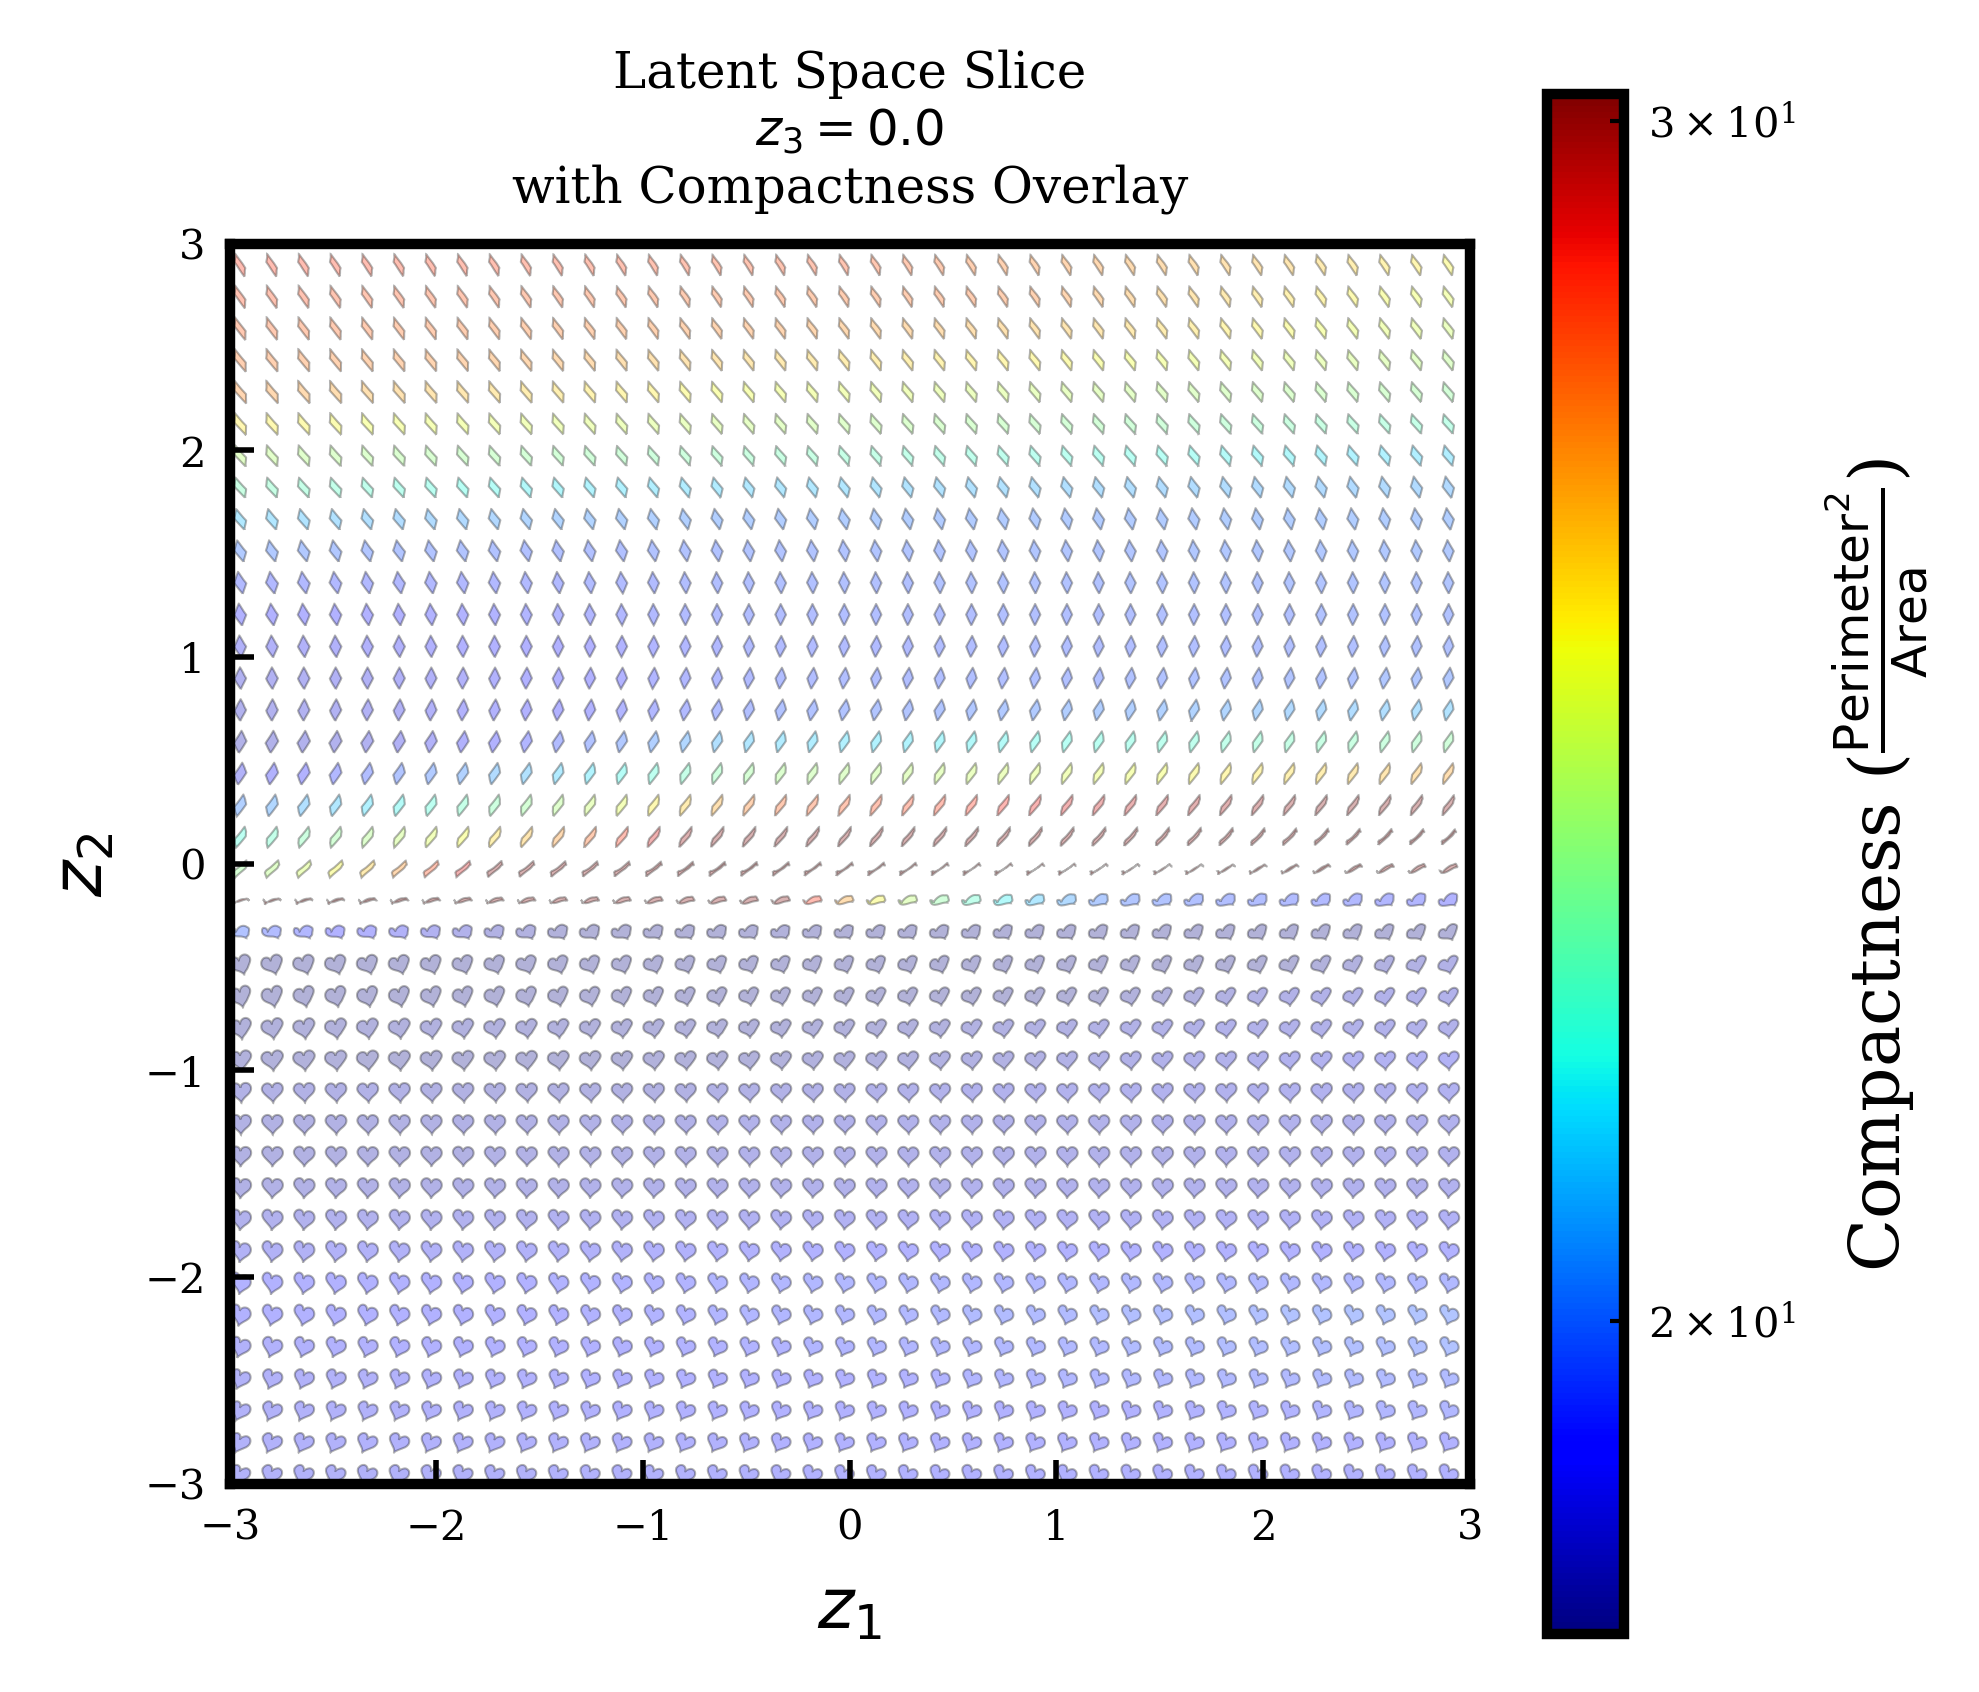
\includegraphics[height=0.3\textheight]{figures/VAEmodels/model2/fix_z3_0.0.png}
    \caption{$Z_3 = 0.0$}
    \label{fig:model2_fixz3_latent}
  \end{subfigure}
  \caption{Model 2 - Latent space visualisation with compactness colourmap.}
  \label{fig:model2_latent_vis}
\end{figure}

\subsubsection{VAE Model 3 - 4D Latent Dimension}
A 4-dimensional VAE is trained, whereby 4 latent dimensions are used to represent the originally high-dimensional 200-node shapes. Increasing the dimension of the latent space provide additional degrees of freedom, adding an additional dimension over which salient information of the original data is stored in the form of a latent value. Despite increasing the latent vector dimension to 4, we maintain the same model architecture (i.e., number of network layers, and nodes per layer), therefore the number of parameters in the network varies insignificantly (see Table~\ref{tab:vae_models}), and is therefore not expected to necessitate a significant increase in data to support effective training of the VAE. The loss curve for the combined MSE and KL-divergence loss shown in Figure~\ref{fig:model3_loss_plot} reveals similar performance to that seen in the 2D latent and 3D VAE models, whereby the loss falls to ~1000 within the first 200 epochs of training and remains stable until the 1000th epoch of training.

\begin{figure}[H]
\centering
    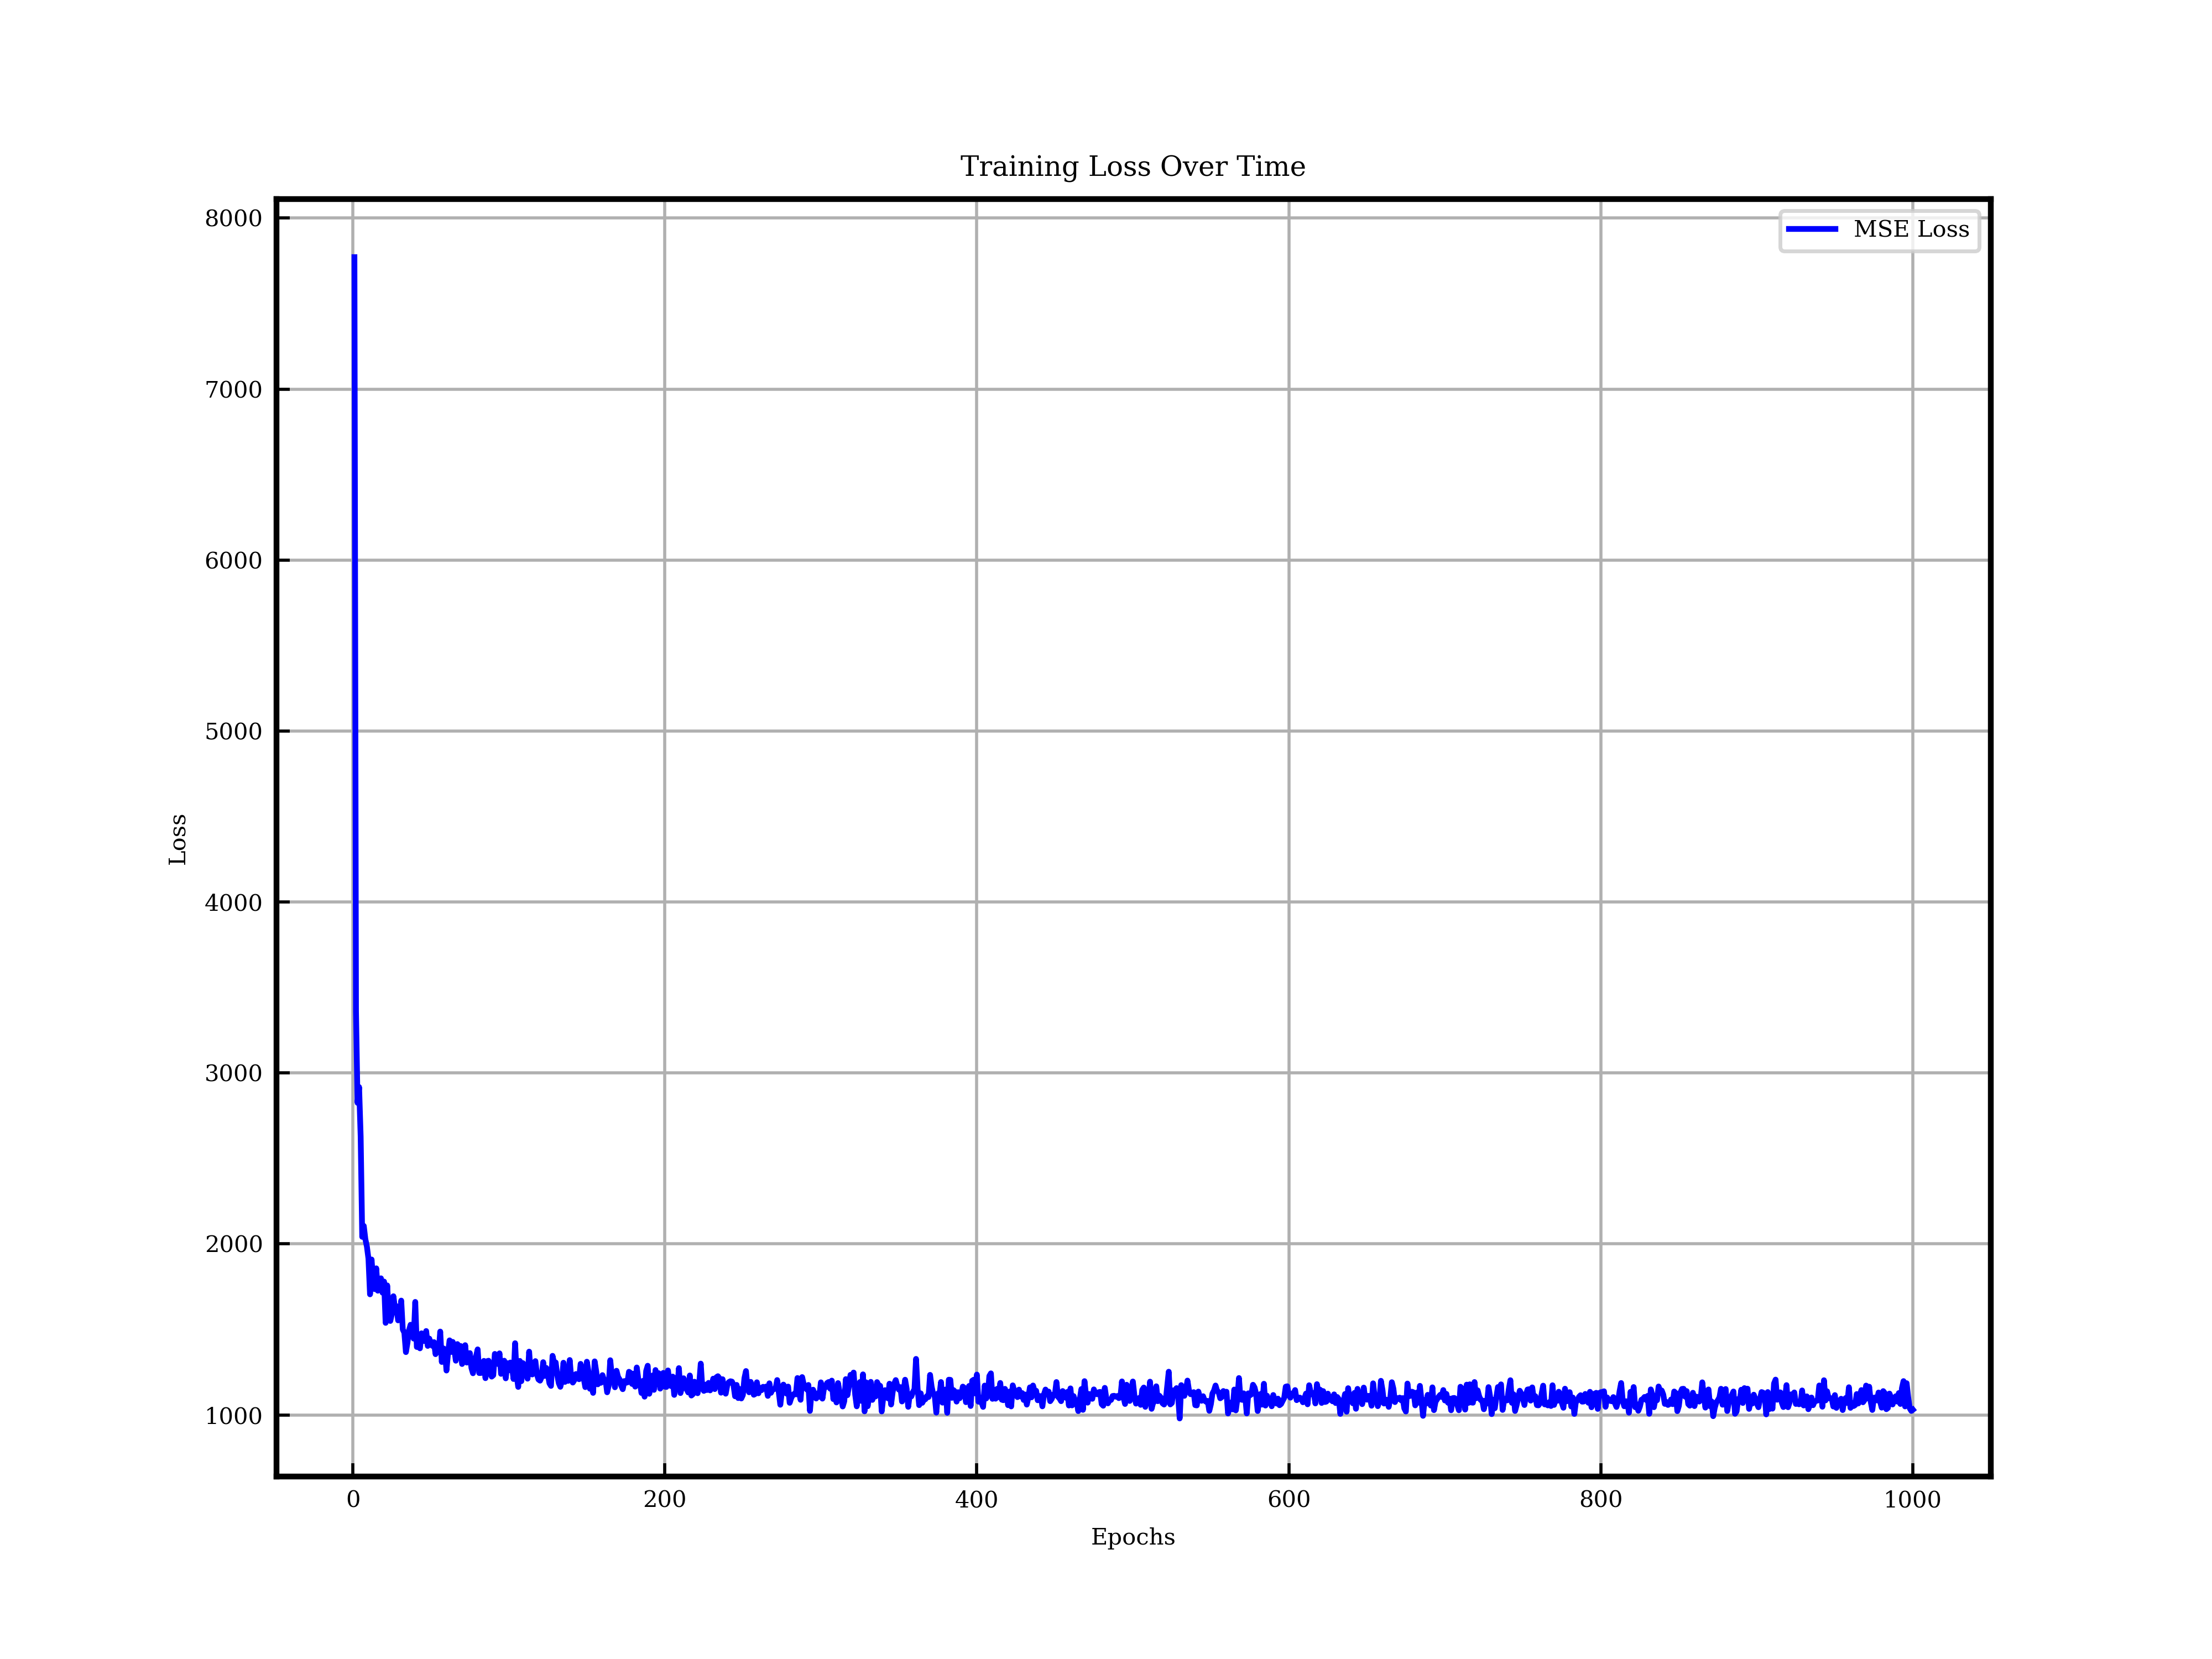
\includegraphics[width=0.75\linewidth]{figures/VAEmodels/model3/loss_plot.png}
    \caption{VAE Model 3 - MSE + KL Loss Plot}
    \label{fig:model3_loss_plot}
\end{figure}

The distribution of all latent values, for each of the latent dimensions are presented in Figure~\ref{fig:model3_latent_dist}. Four latent distributions are present, with latent dimension $Z_4$ and $Z_1$ demonstrating almost identical distributions of latent values, while $Z_2$ is characterised by multiple peaks at across the range. Latent dimension $Z_3$ shows shoulders in the distributions around -1.75, and +1.75. Despite the multi-modal features of the distributions, all latent values are centralised around 0 in accordance with the standard normal prior placed on the latent-distribution as described in \ref{prior_dist}. To avoid overburdening the reader with all combinations of fixed latent vectors while visualising the remaining dimensions in 2D, from this point on we direct the reader to the appendix for all resultant VAE generated latent spaces. For models with 4 latent dimensions, there are 6 combinations for which we could visualise, though we opt to demonstrate the most informative and pertinent latent visualisations to emphasise the effect of changing the number of latent dimensions and the implications on downstream use cases. Figure~\ref{fig:model3_fixz1z4} presents the resultant shapes generated when sampling across latent dimensions $Z_3$ and $Z_2$ while fixing $Z_1$ and $Z_4$ at 0. There is little visual difference apparent from those shown for the 2D and 3D VAE models. The performance surface is smooth and continuous, demonstrating a complex surface with various local optima. Over the range of visualised latent vector values, we can identify most of the original shape categories used as part of the training process, including squares, triangles, diamonds, pentagons, hearts and stars. Circles do not clearly emerge over the generated latent values. The remaining pairings of VAE latent dimensions do not demonstrate significant variation across the sampled latent ranges, therefore we exclude these and refer the reader to the appendix.


\begin{figure}[H]
    \centering
    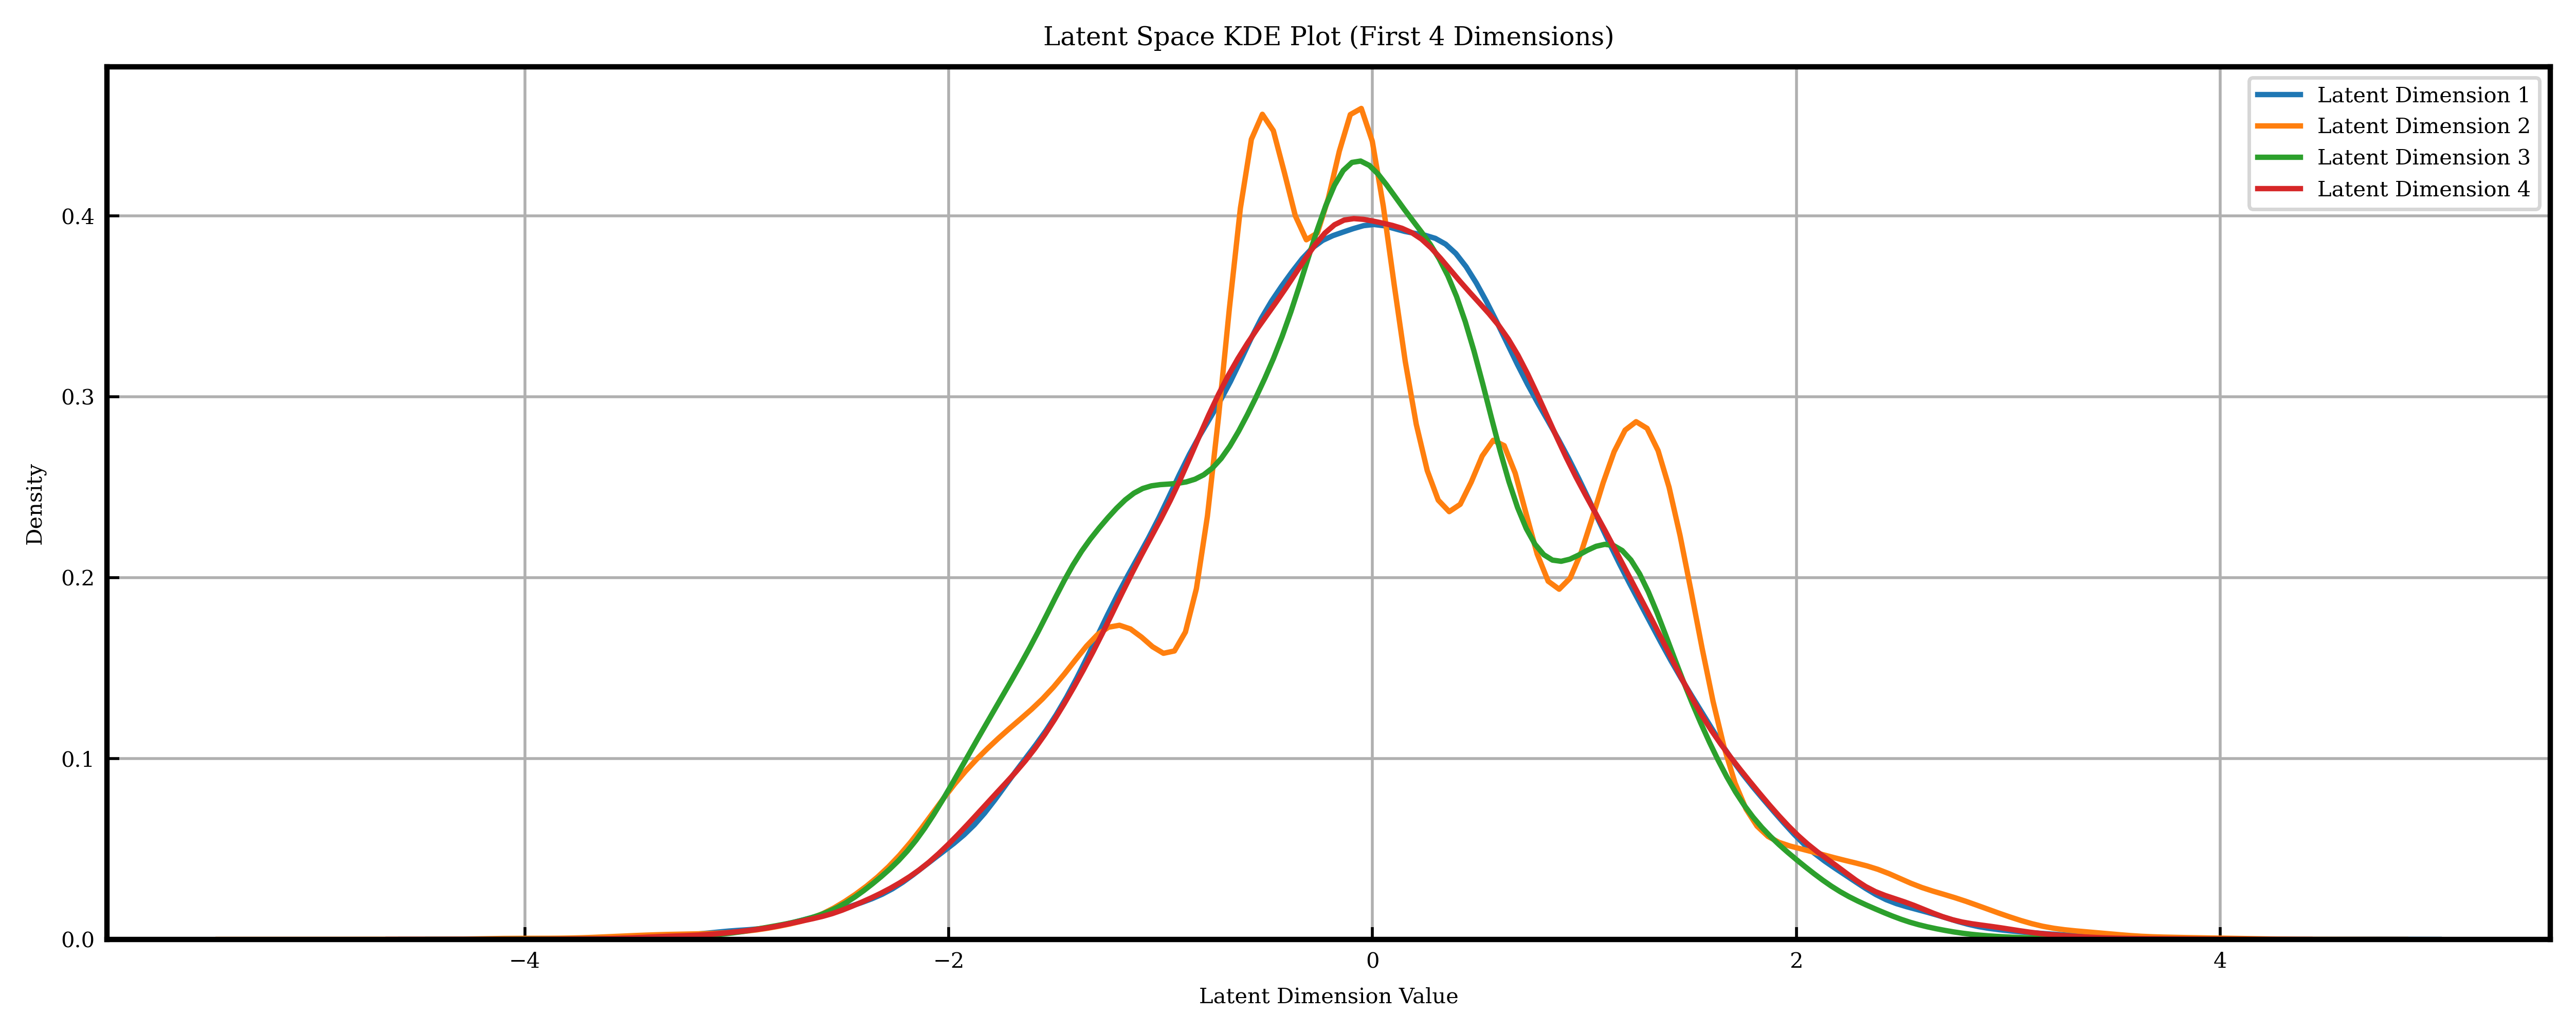
\includegraphics[width=0.75\linewidth]{figures/VAEmodels/model3/latent_distribution.png}
    \caption{Model 3 - Latent dimension distributions over all training data}
    \label{fig:model3_latent_dist}
\end{figure}

The generated shapes shown in Figure~\ref{fig:model3_fixz1z4} reveal reveal clusters whereby the performance metric has little to no change over regions of the latent space. For example, for $Z_1$ and $Z_2$ between [-3,-1] squares dominate the generated shape population, however, across this range there is no obvious sign of variation between the squares shape, neither is there any change in the compactness value. In other regions, such example $Z_3$ = [-3,-1] and $Z_2$ = [[1,3] there is a clear transition from a pentagon-like shape in the top left, down to a compressed star like structure in the bottom right with a more prominent change in the compactness value represented by the gradient of the colormap. Interpolating through this region of the latent dimensions results in increased discovery of novel shapes; a desirable characteristic in design space exploration. Deploying, for example, gradient based optimisation through finite-difference exploration would enable navigation towards an optimal compactness value, whereas for the square region, there is little performance gain to be realised, therefore the volume of the design space would need to be increase to reliably identify varying designs.


\begin{figure}[H]
  \centering

  \begin{subfigure}{0.48\textwidth}
    \centering
    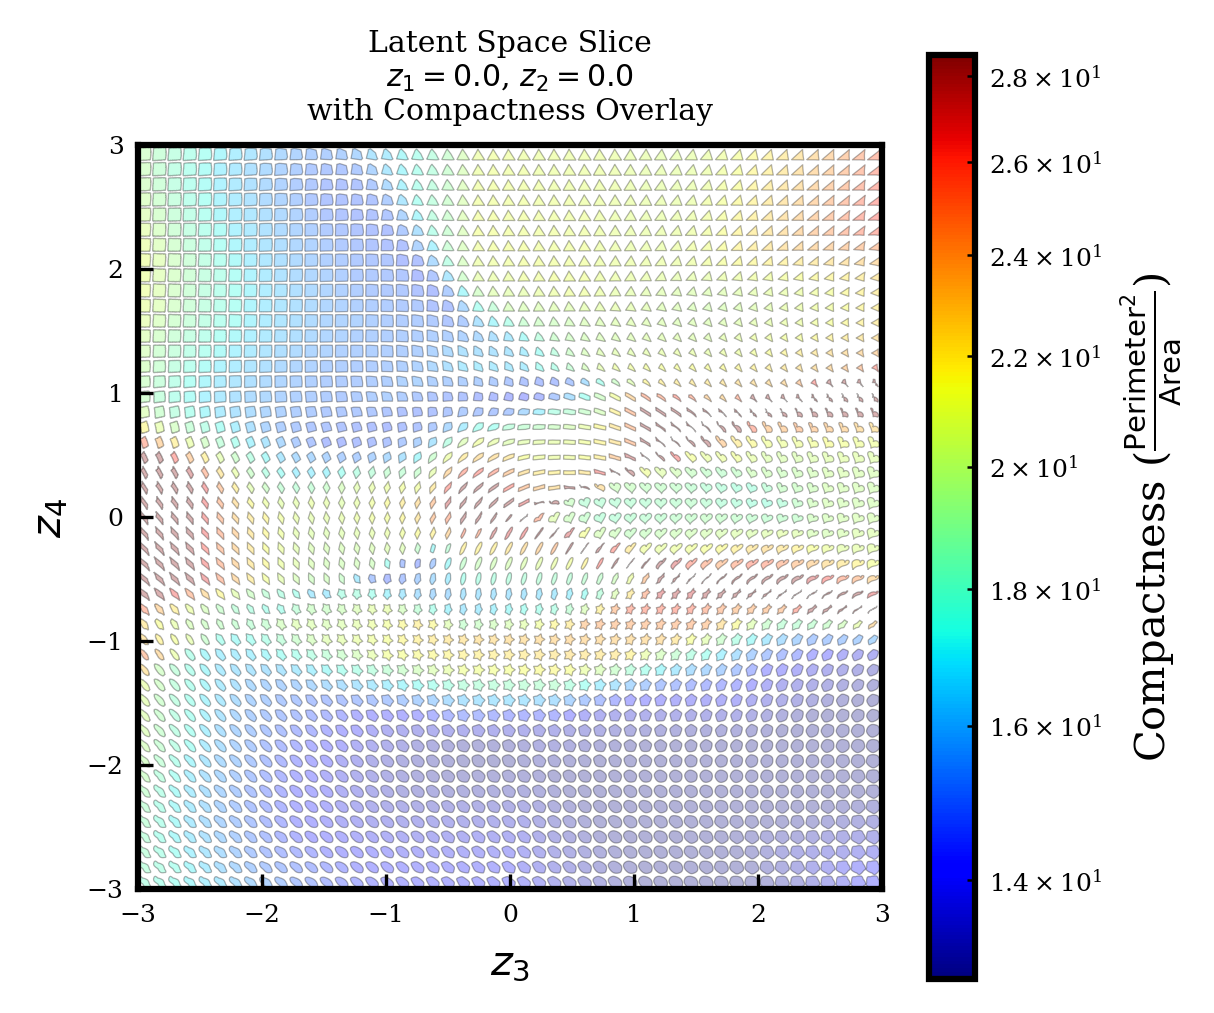
\includegraphics[width=\textwidth]{figures/VAEmodels/model3/varying_z3_z4_fixed_z1=0.0_z2=0.0.png}
    \caption{Latent dimensions $Z_3$ and $Z_4$}
    \label{fig:model3_z3_z4}
  \end{subfigure}
  \hfill
  \begin{subfigure}{0.48\textwidth}
    \centering
    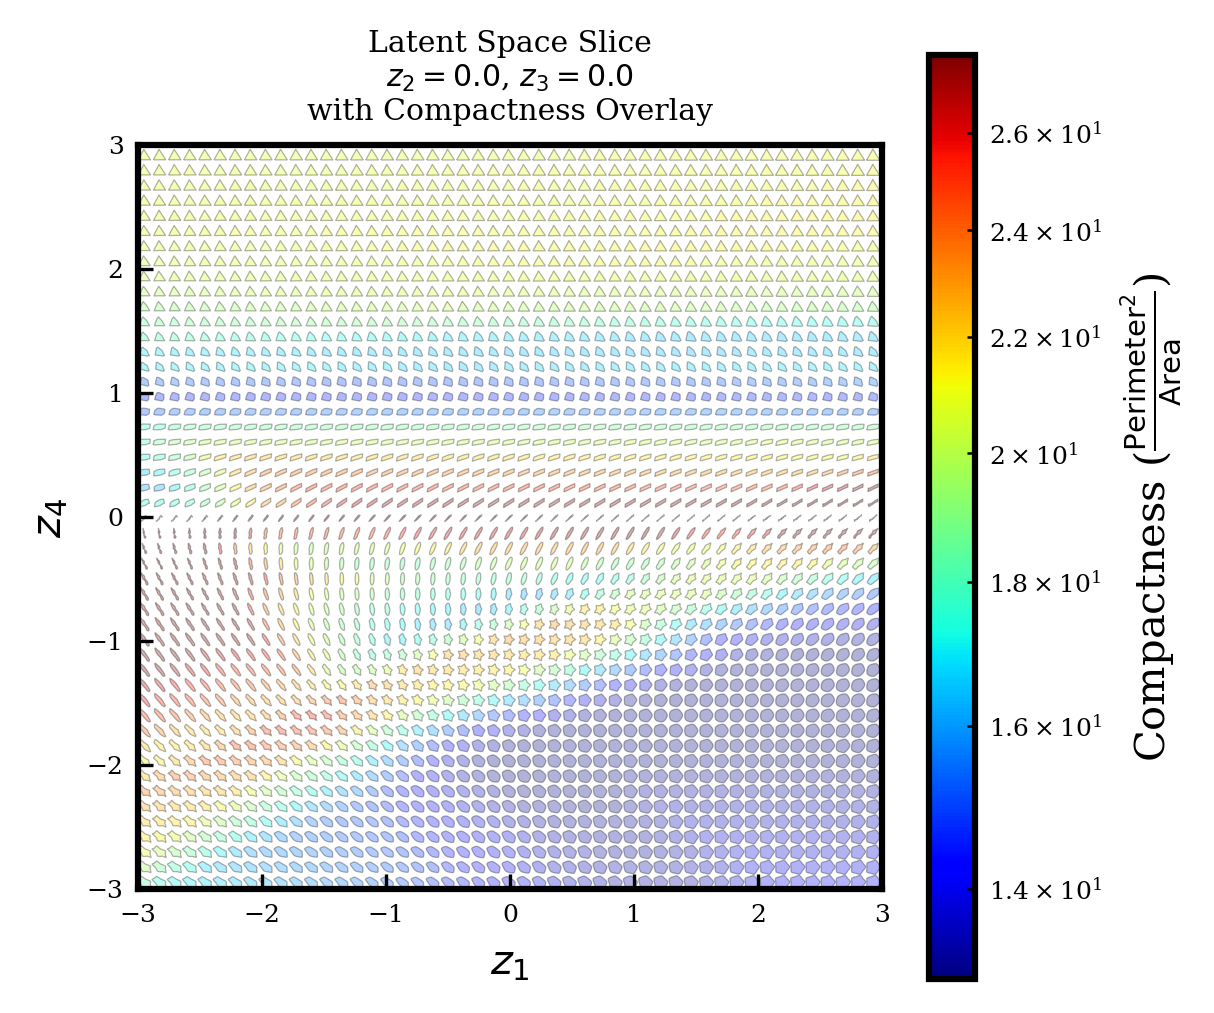
\includegraphics[width=\textwidth]{figures/VAEmodels/model3/varying_z1_z4_fixed_z2=0.0_z3=0.0.png}
    \caption{Latent dimensions $Z_1$ and $Z_4$}
    \label{fig:model3_z1_z4}
  \end{subfigure}

  \vspace{0.5em}

  \begin{subfigure}{0.48\textwidth}
    \centering
    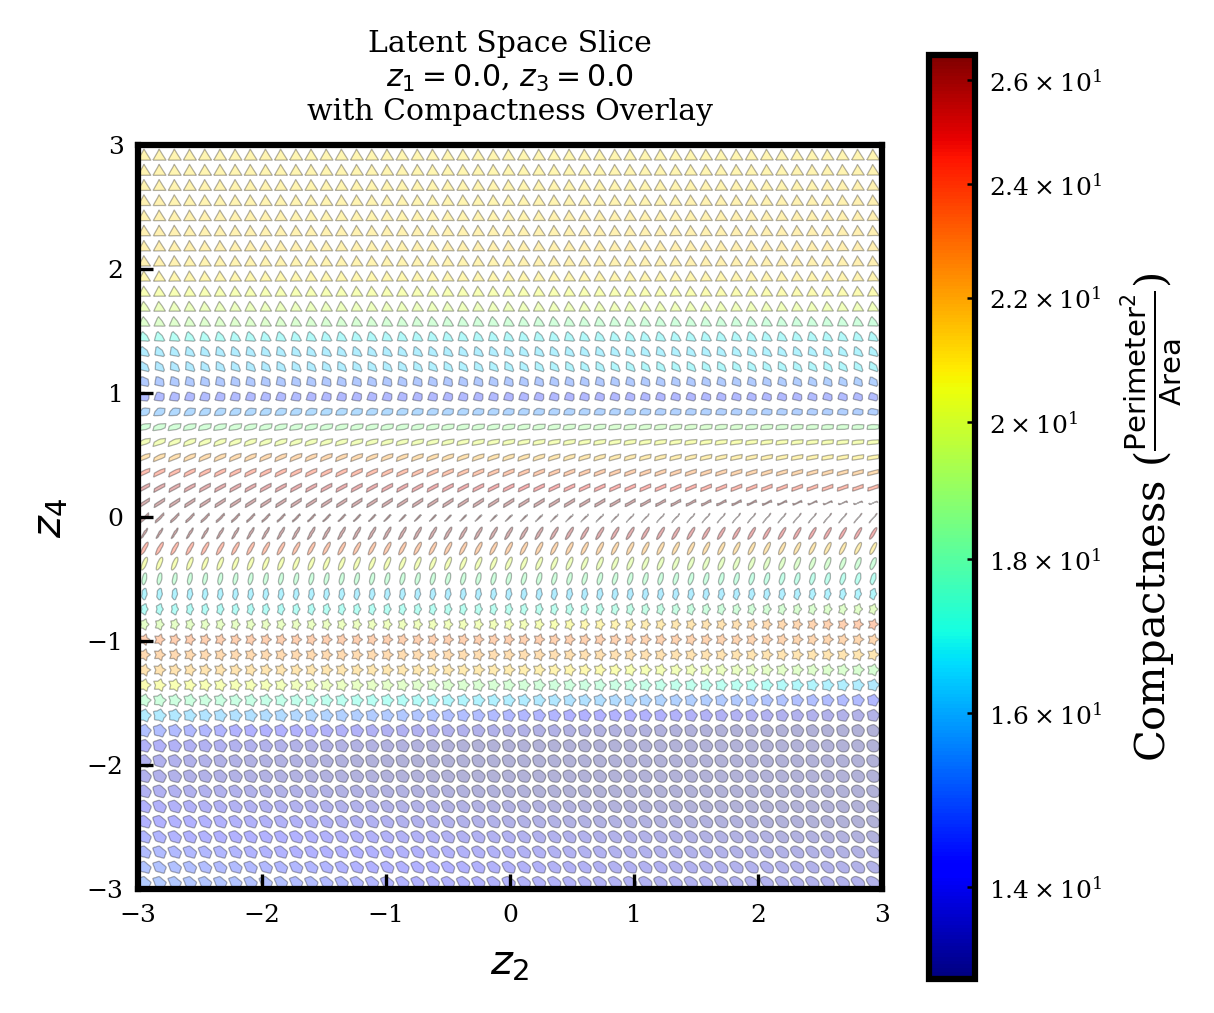
\includegraphics[width=\textwidth]{figures/VAEmodels/model3/varying_z2_z4_fixed_z1=0.0_z3=0.0.png}
    \caption{Latent dimensions $Z_2$ and $Z_4$}
    \label{fig:model3_z2_z4}
  \end{subfigure}
  \hfill
  \begin{subfigure}{0.48\textwidth}
    \centering
    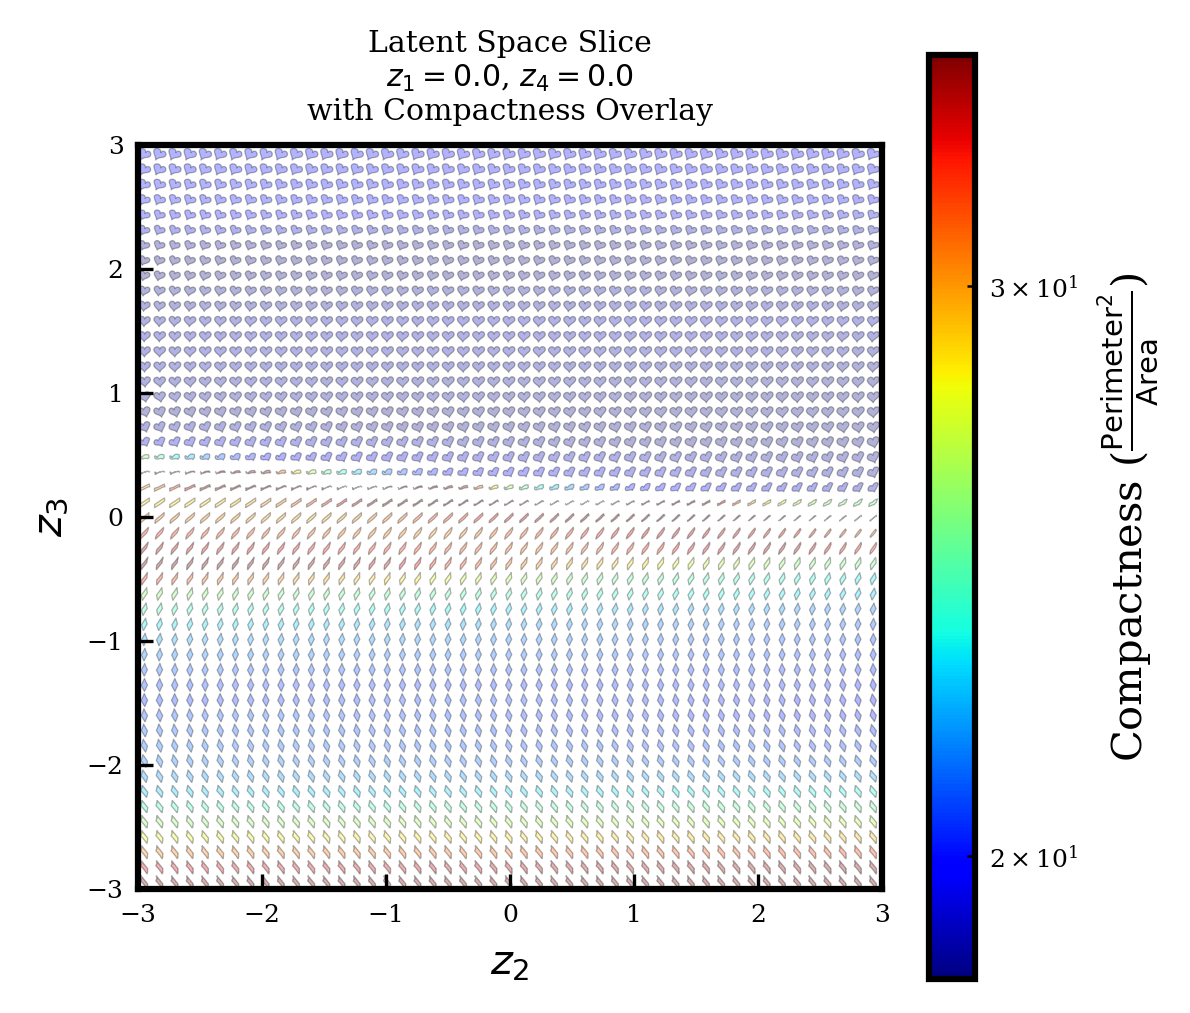
\includegraphics[width=\textwidth]{figures/VAEmodels/model3/varying_z2_z3_fixed_z1=0.0_z4=0.0.png}
    \caption{Latent dimensions $Z_2$ and $Z_3$}
    \label{fig:model3_z2_z3}
  \end{subfigure}

  \caption{Model 3 - Latent space visualisation with compactness colourmap.}
  \label{fig:model3_latent_visualisations}
\end{figure}


\subsubsection{VAE Model 4 - 5D Latent Dimension}

Model 4 expands upon the previous with an additional latent dimension, for a total of 5 dimensions. As previously demonstrated, the sole addition of an extra dimension in the bottleneck layer of the VAE does not significantly increase the size of the model architecture with respect to to model parameters, and as a result, the training phase of the VAE exhibits almost identical performance to models with lesser numbers of dimensions - this is shown in Figure~\ref{fig:model4_loss_plot}, with a combined MSE + KL-divergence loss of ~1000 after 200 epochs. For 5 dimensions, there are 10 possible combinations of visualising the generated latent shapes over 2 latent dimensions, therefore again, we refer the reader to the appendix for the full set.

\begin{figure}[H]
\centering
    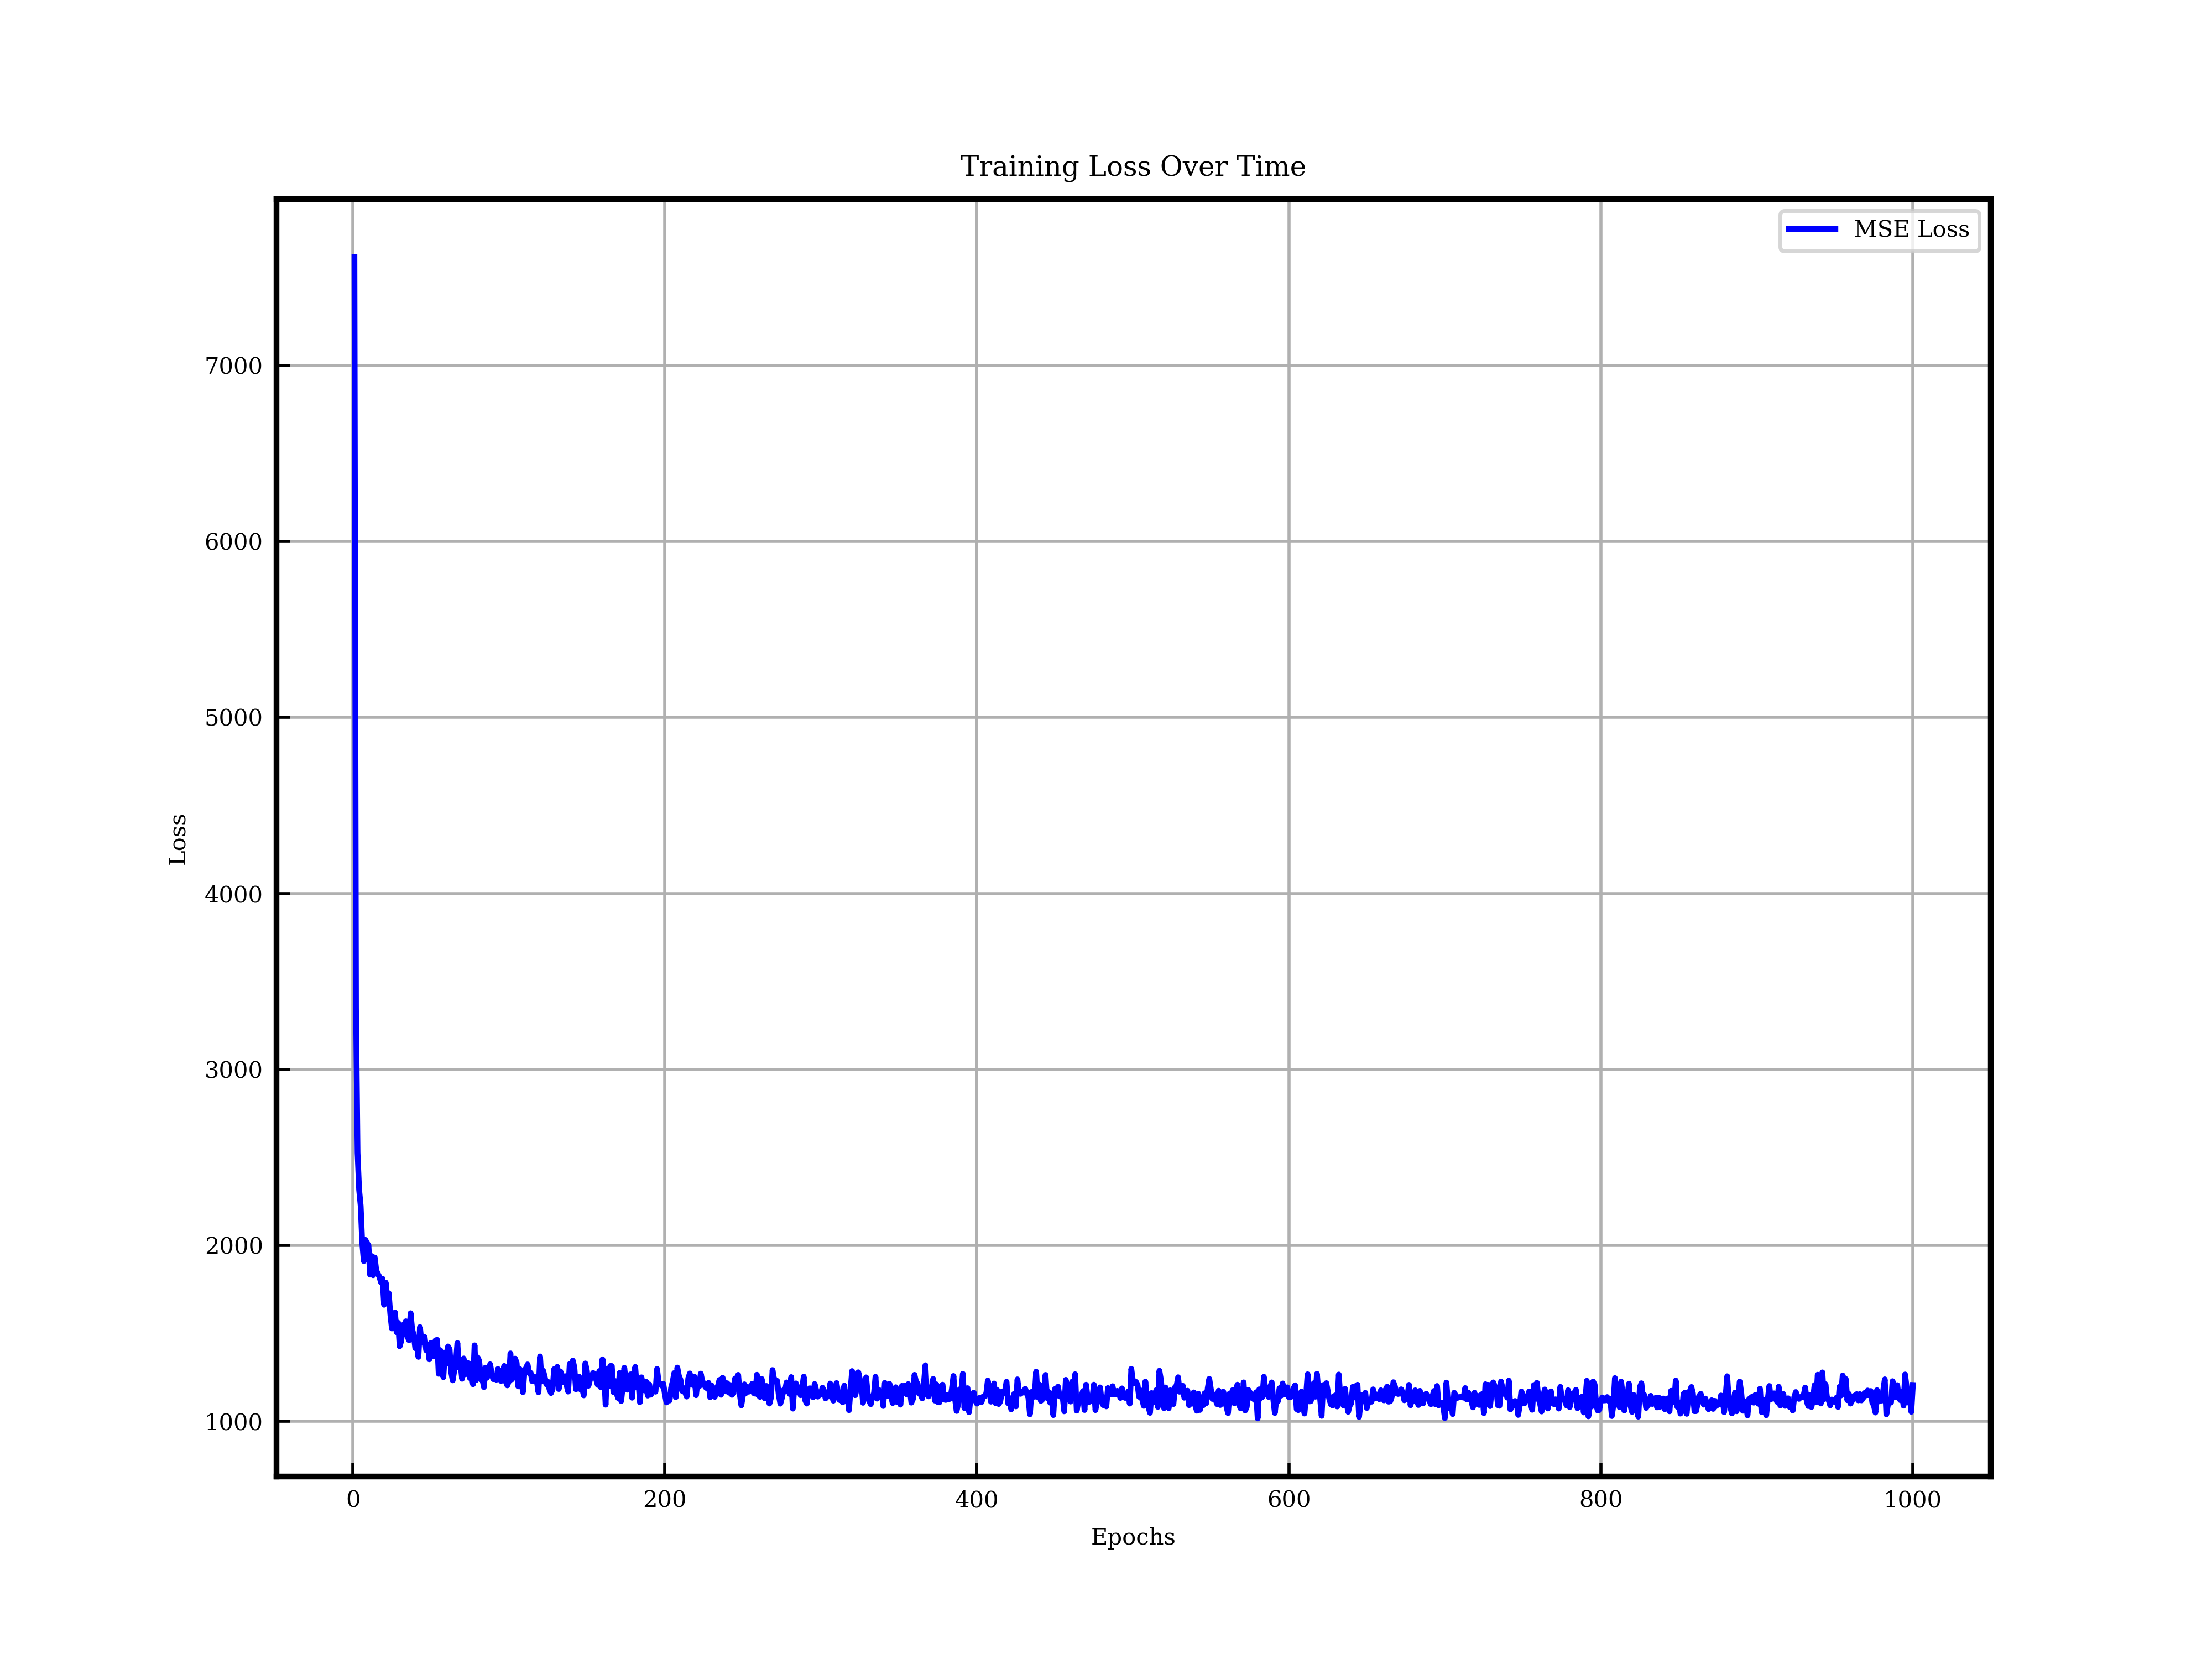
\includegraphics[width=0.75\linewidth]{figures/VAEmodels/model4/loss_plot.png}
    \caption{VAE Model 4 - MSE + KL Loss Plot}
    \label{fig:model4_loss_plot}
\end{figure}

We present the distribution over all 5 dimensions when encoding all 100,000 training shapes. The distribution of latent values for each of the dimensions is shown in Figure~\ref{fig:model4_latent_dist}. The most unique distribution is observed for latent dimension 3, whereby there are peaks around values of 0 and 1, with a shoulder also evident at -2. The remaining latent dimensions show similar distribution centred around 0. The range of z values across all latent dimensions remains similar, not exceeding above or below 4 and -4 respectively.

\begin{figure}[H]
    \centering
    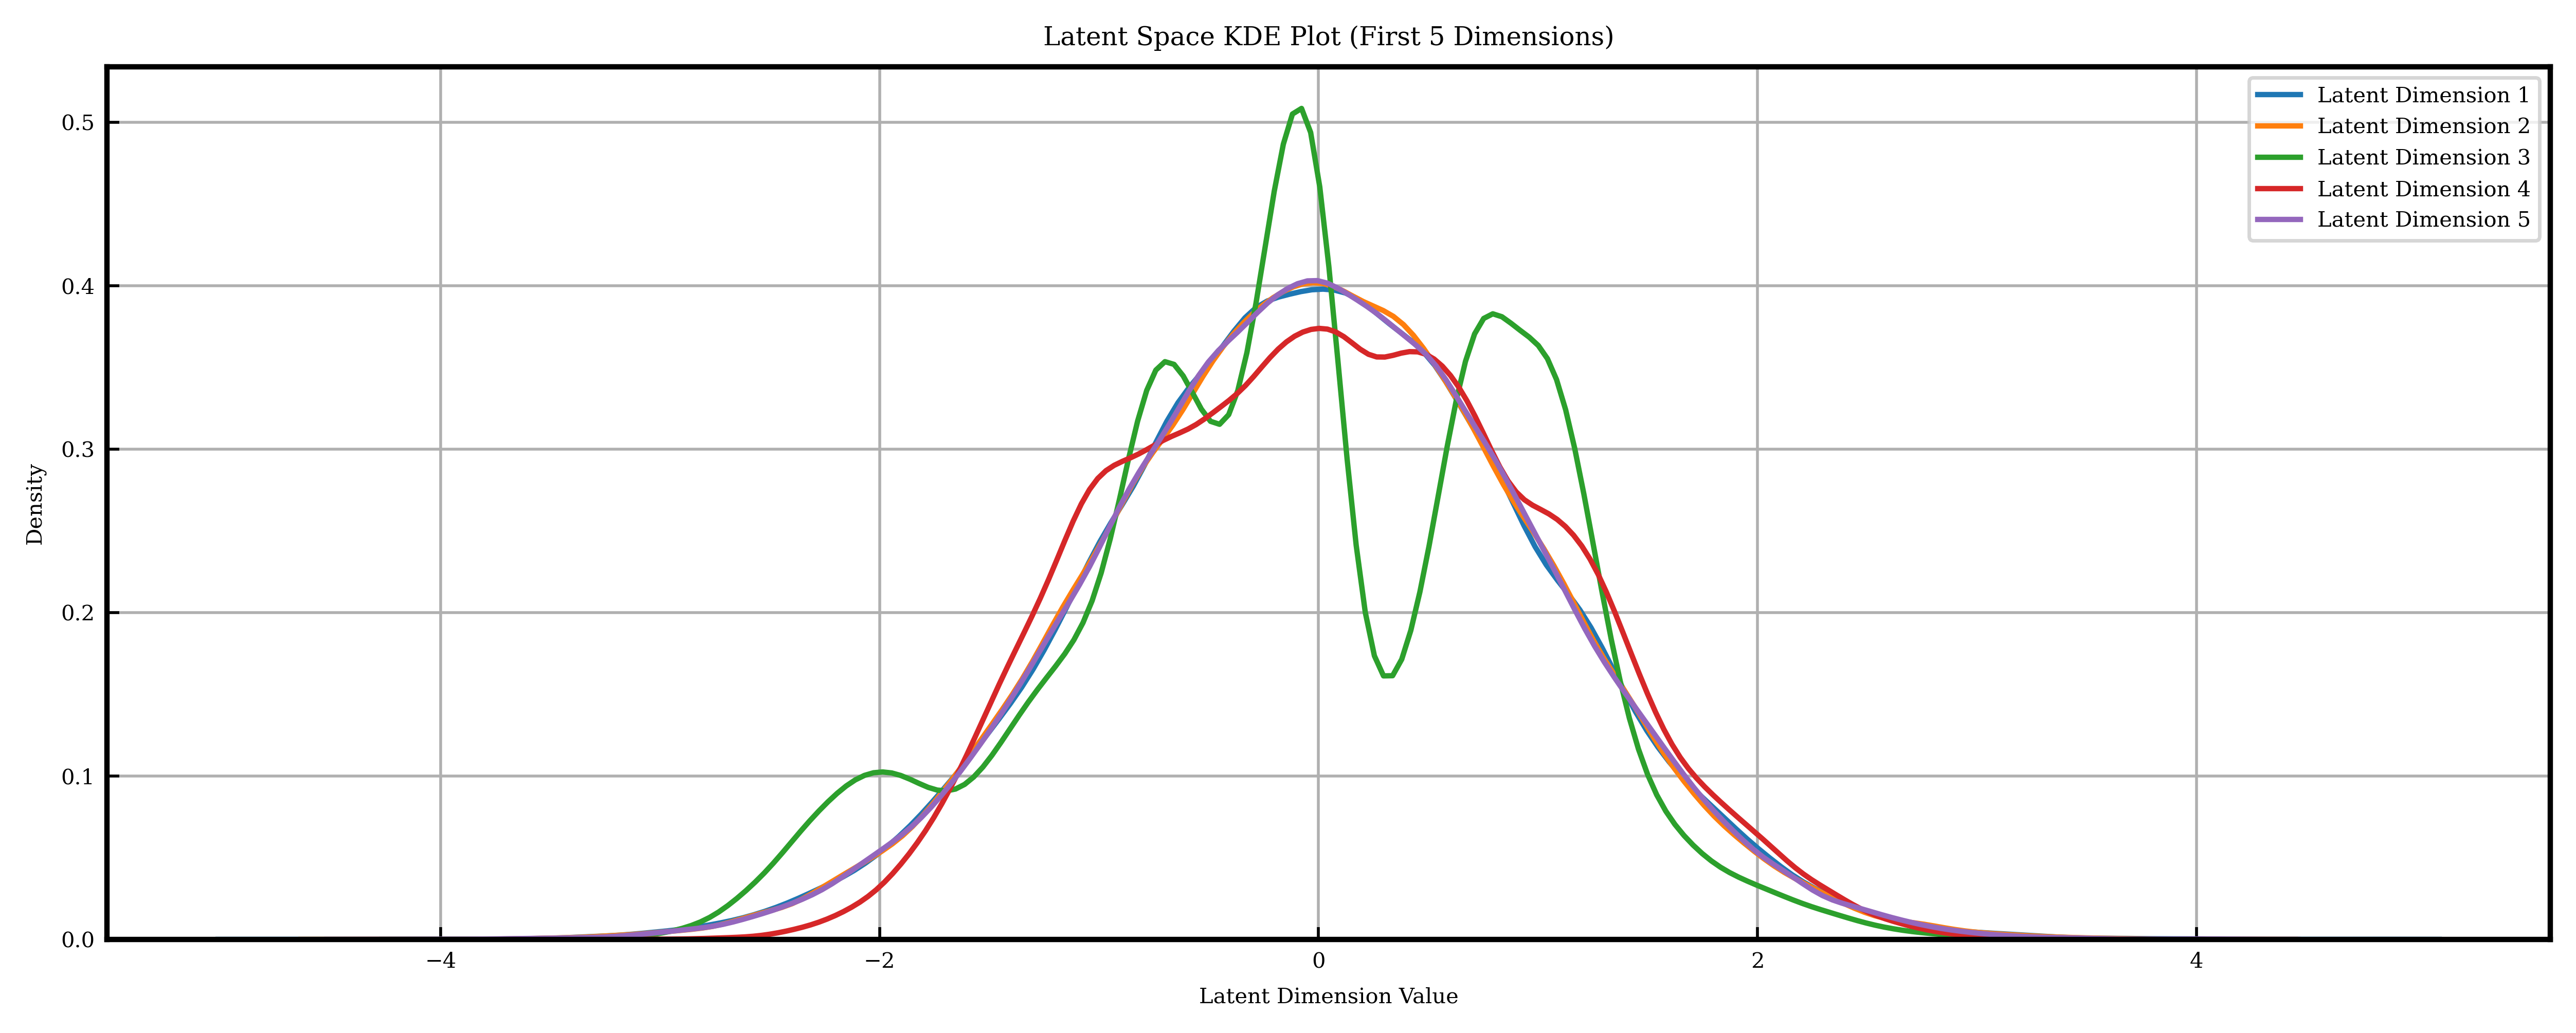
\includegraphics[width=0.75\linewidth]{figures/VAEmodels/model4/latent_distribution.png}
    \caption{Model 4 - Latent dimension distributions over all training data}
    \label{fig:model4_latent_dist}
\end{figure}

We present 4 combinations of latent dimensions that demonstrate the greatest variance in 1) shape diversity, and 2) range of compactness values across the generated shape range. These can be in seen in Figure~\ref{fig:model4_latent_visualisations}. Following trend for the previous VAE models, one single configuration of two latent dimensions results in the most expressive latent space, with the largest variance in the shapes generated across the sampled z-value range and most complex performance surface in terms of the compactness metric. Figure~\ref{fig:model4_z2_z4} demonstrates a complex performance surface that has variation in the generated shapes across both $Z_2$ and $Z_4$ dimensions. In contrast, Figure~\ref{fig:model4_z2_z3} exhibits banding where navigation through the $Z_3$ latent dimension yields little to no change in the generated shapes and resultant compactness - this is represented as vertical bands across the generated  shapes. Meanwhile, in Figure~\ref{fig:model4_z1_z5}, the generated shapes appear very similar in geometry terms, though there is a gradual, but present gradient in the compactness metrics across the range, suggesting a subtle change in the geometry, that is represented in a changing compactness value. In this example, interpolation through the latent space does not yield diversity in the generated designs, though does exhibit favourable smoothness and continuity characteristics. Similarly to Figure~\ref{fig:model4_z2_z3}, Figure~\ref{fig:model4_z1_z2} demonstrates banding through the latent space, whereby movement in the $Z_1$ dimensions does not result in any change in shape while interpolating through the $Z_2$ dimension demonstrates a transition from triangles at $Z_2=-3$ to pentagon and circle-like geometries between $Z_1=[1,3]$. 


\begin{figure}[H]
  \centering

  \begin{subfigure}{0.48\textwidth}
    \centering
    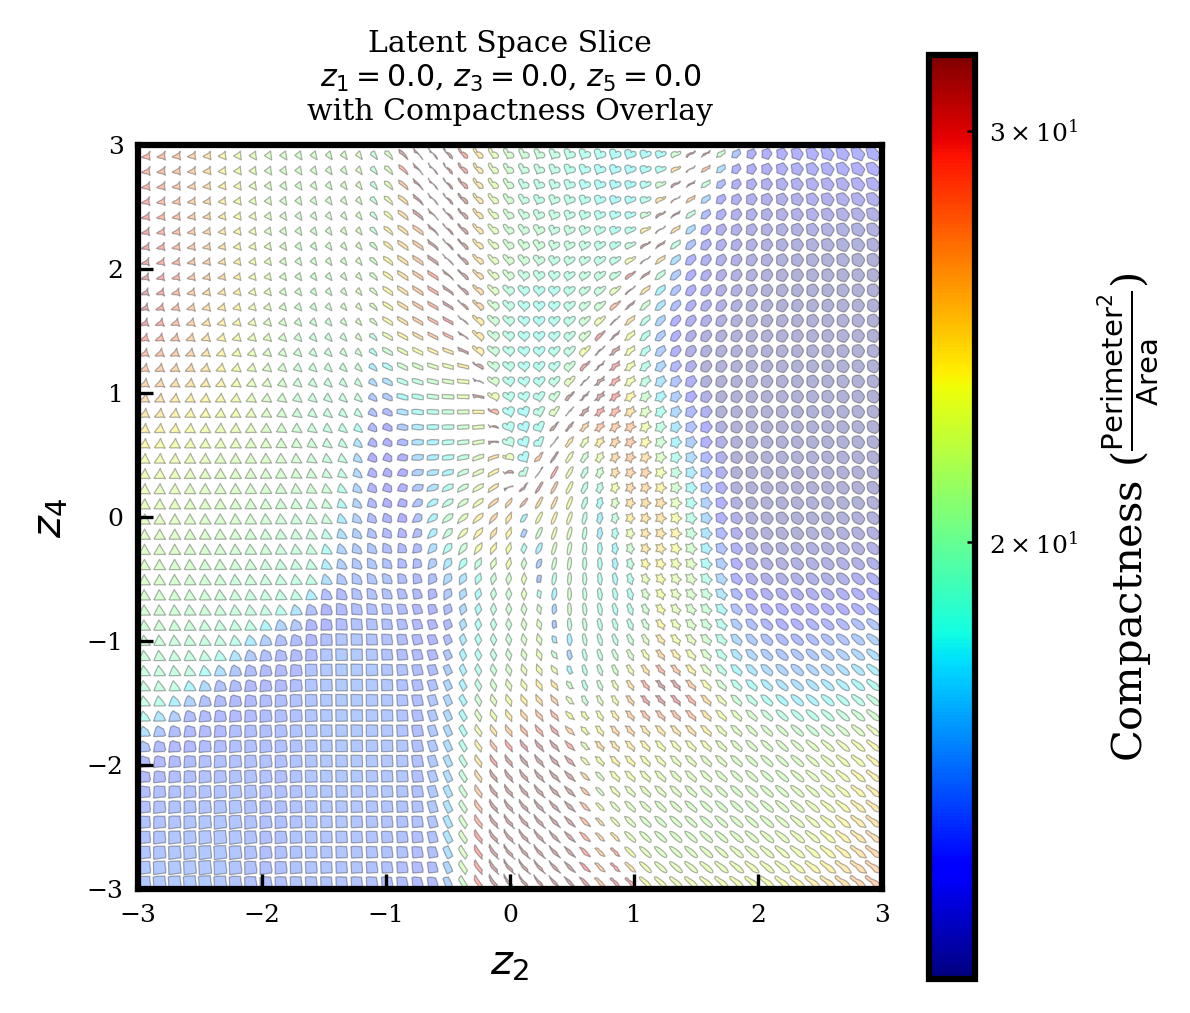
\includegraphics[width=\textwidth]{figures/VAEmodels/model4/varying_z2_z4_fixed_z1=0.0_z3=0.0_z5=0.0.png}
    \caption{Latent dimensions $Z_2$ and $Z_4$}
    \label{fig:model4_z2_z4}
  \end{subfigure}
  \hfill
  \begin{subfigure}{0.48\textwidth}
    \centering
    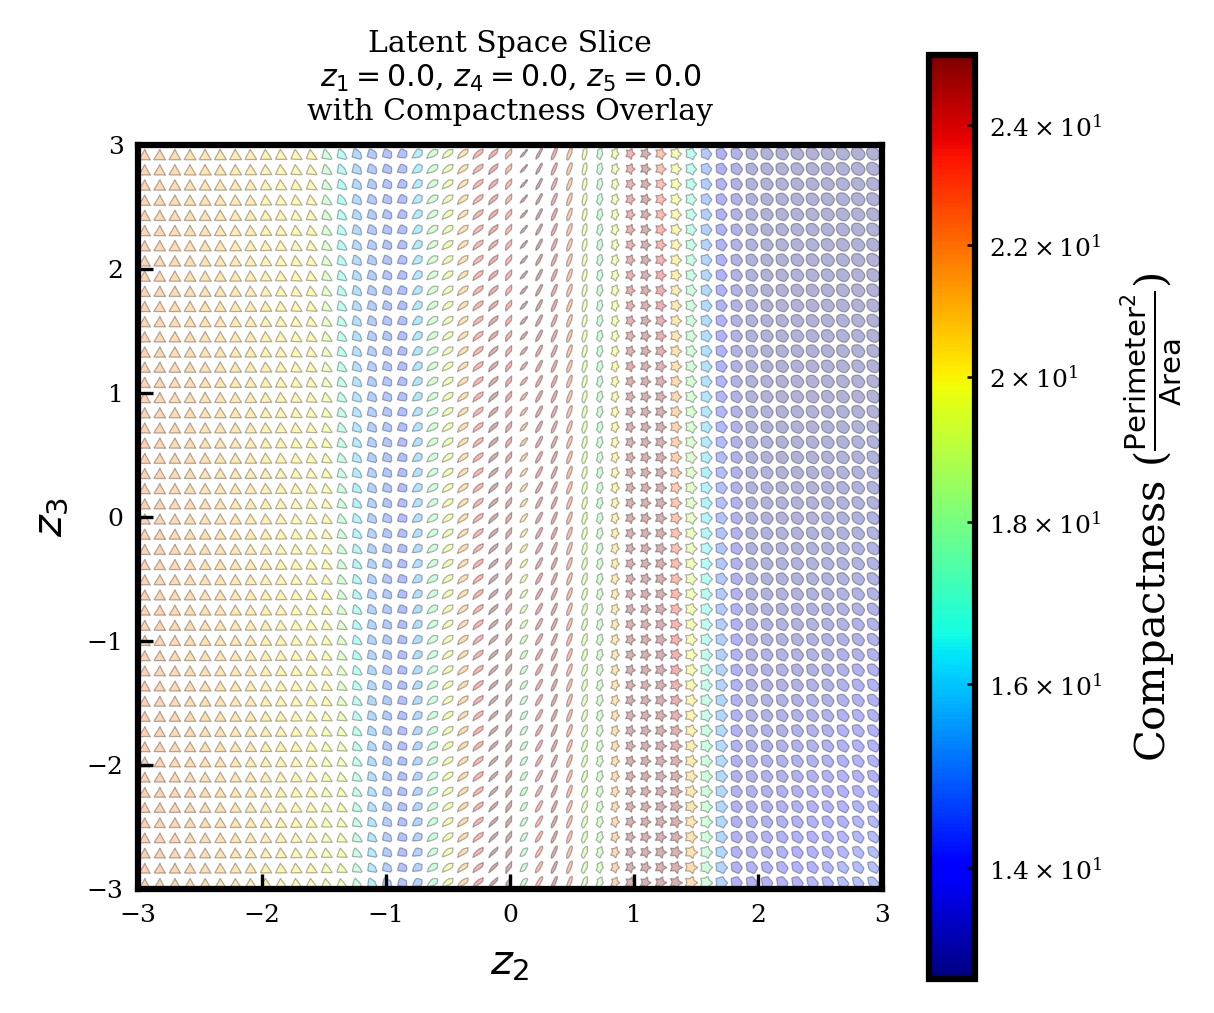
\includegraphics[width=\textwidth]{figures/VAEmodels/model4/varying_z2_z3_fixed_z1=0.0_z4=0.0_z5=0.0.png}
    \caption{Latent dimensions $Z_2$ and $Z_3$}
    \label{fig:model4_z2_z3}
  \end{subfigure}

  \vspace{0.5em}

  \begin{subfigure}{0.48\textwidth}
    \centering
    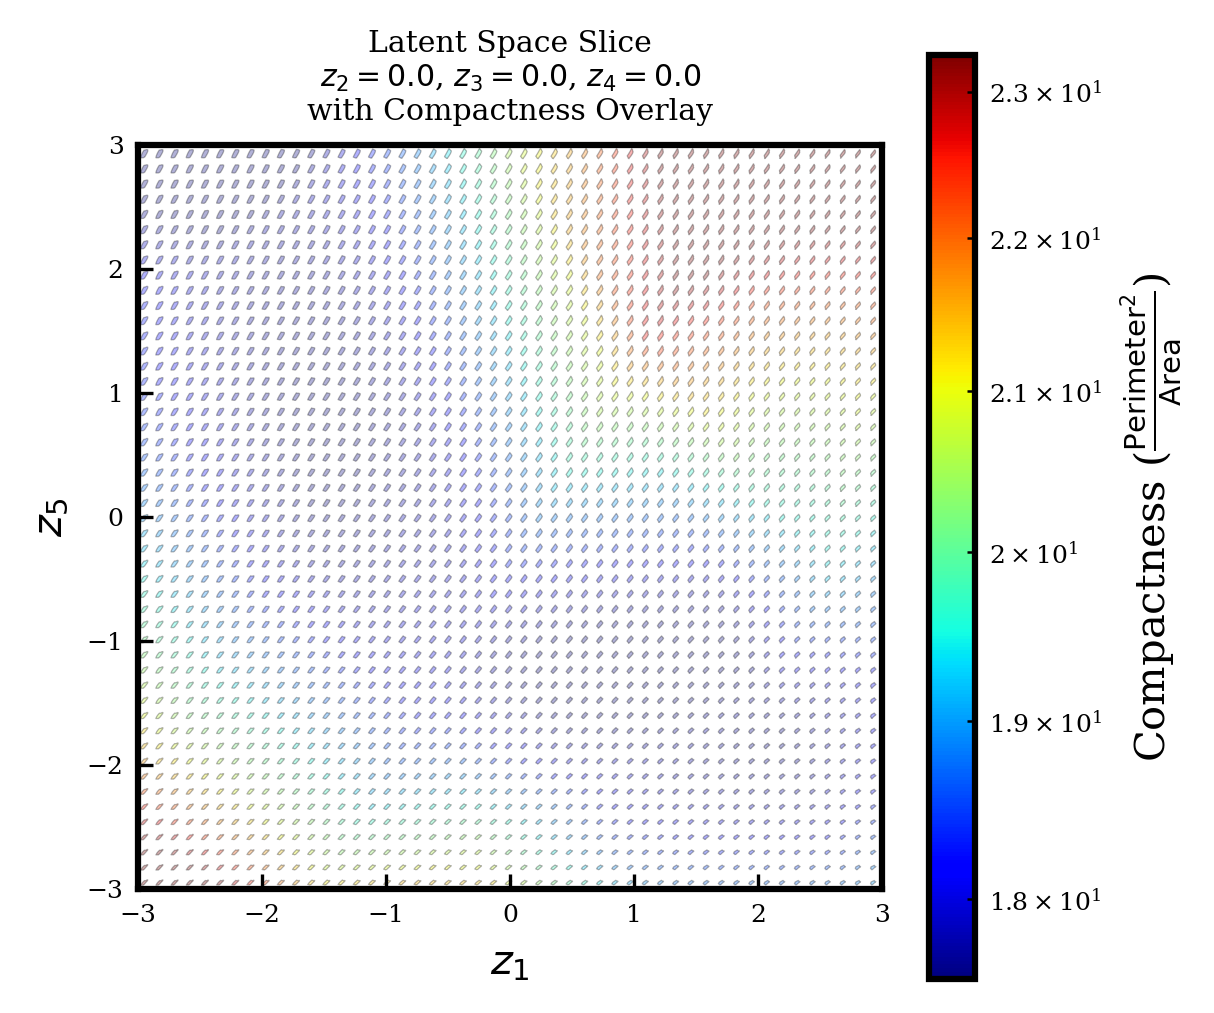
\includegraphics[width=\textwidth]{figures/VAEmodels/model4/varying_z1_z5_fixed_z2=0.0_z3=0.0_z4=0.0.png}
    \caption{Latent dimensions $Z_1$ and $Z_5$}
    \label{fig:model4_z1_z5}
  \end{subfigure}
  \hfill
  \begin{subfigure}{0.48\textwidth}
    \centering
    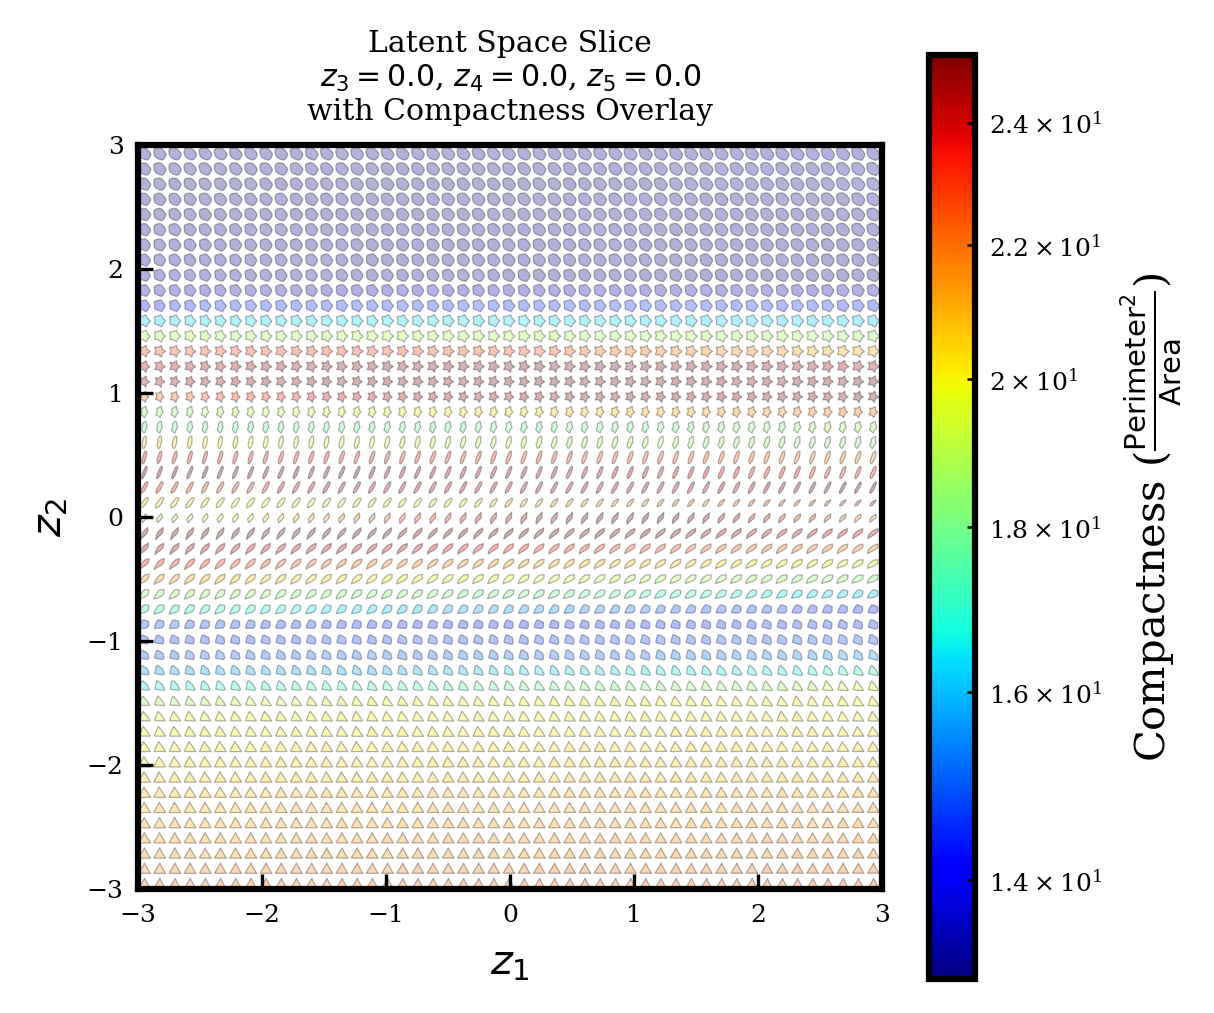
\includegraphics[width=\textwidth]{figures/VAEmodels/model4/varying_z1_z2_fixed_z3=0.0_z4=0.0_z5=0.0.png}
    \caption{Latent dimensions $Z_1$ and $Z_2$}
    \label{fig:model4_z1_z2}
  \end{subfigure}

  \caption{Model 4 - Latent space visualisation with compactness colourmap.}
  \label{fig:model4_latent_visualisations}
\end{figure}


\subsubsection{VAE Model 5 - 6D Latent Dimension}

Finally, VAE model 5 utilises 6 latent dimensions in the bottleneck layer. The addition of an additional dimensions increases the level of expressiveness the latent vector maintains, while minimises the amount of compression of the original dataset, while still providing efficiency enabling dimensionality reduction suitable for downstream use cases. The model training is identical to that of the previous reported models, reaching a combined MSE \& KL-divergence loss of ~1000 for a batch size of 512, plateauing after 200 epochs.

\begin{figure}[H]
\centering
    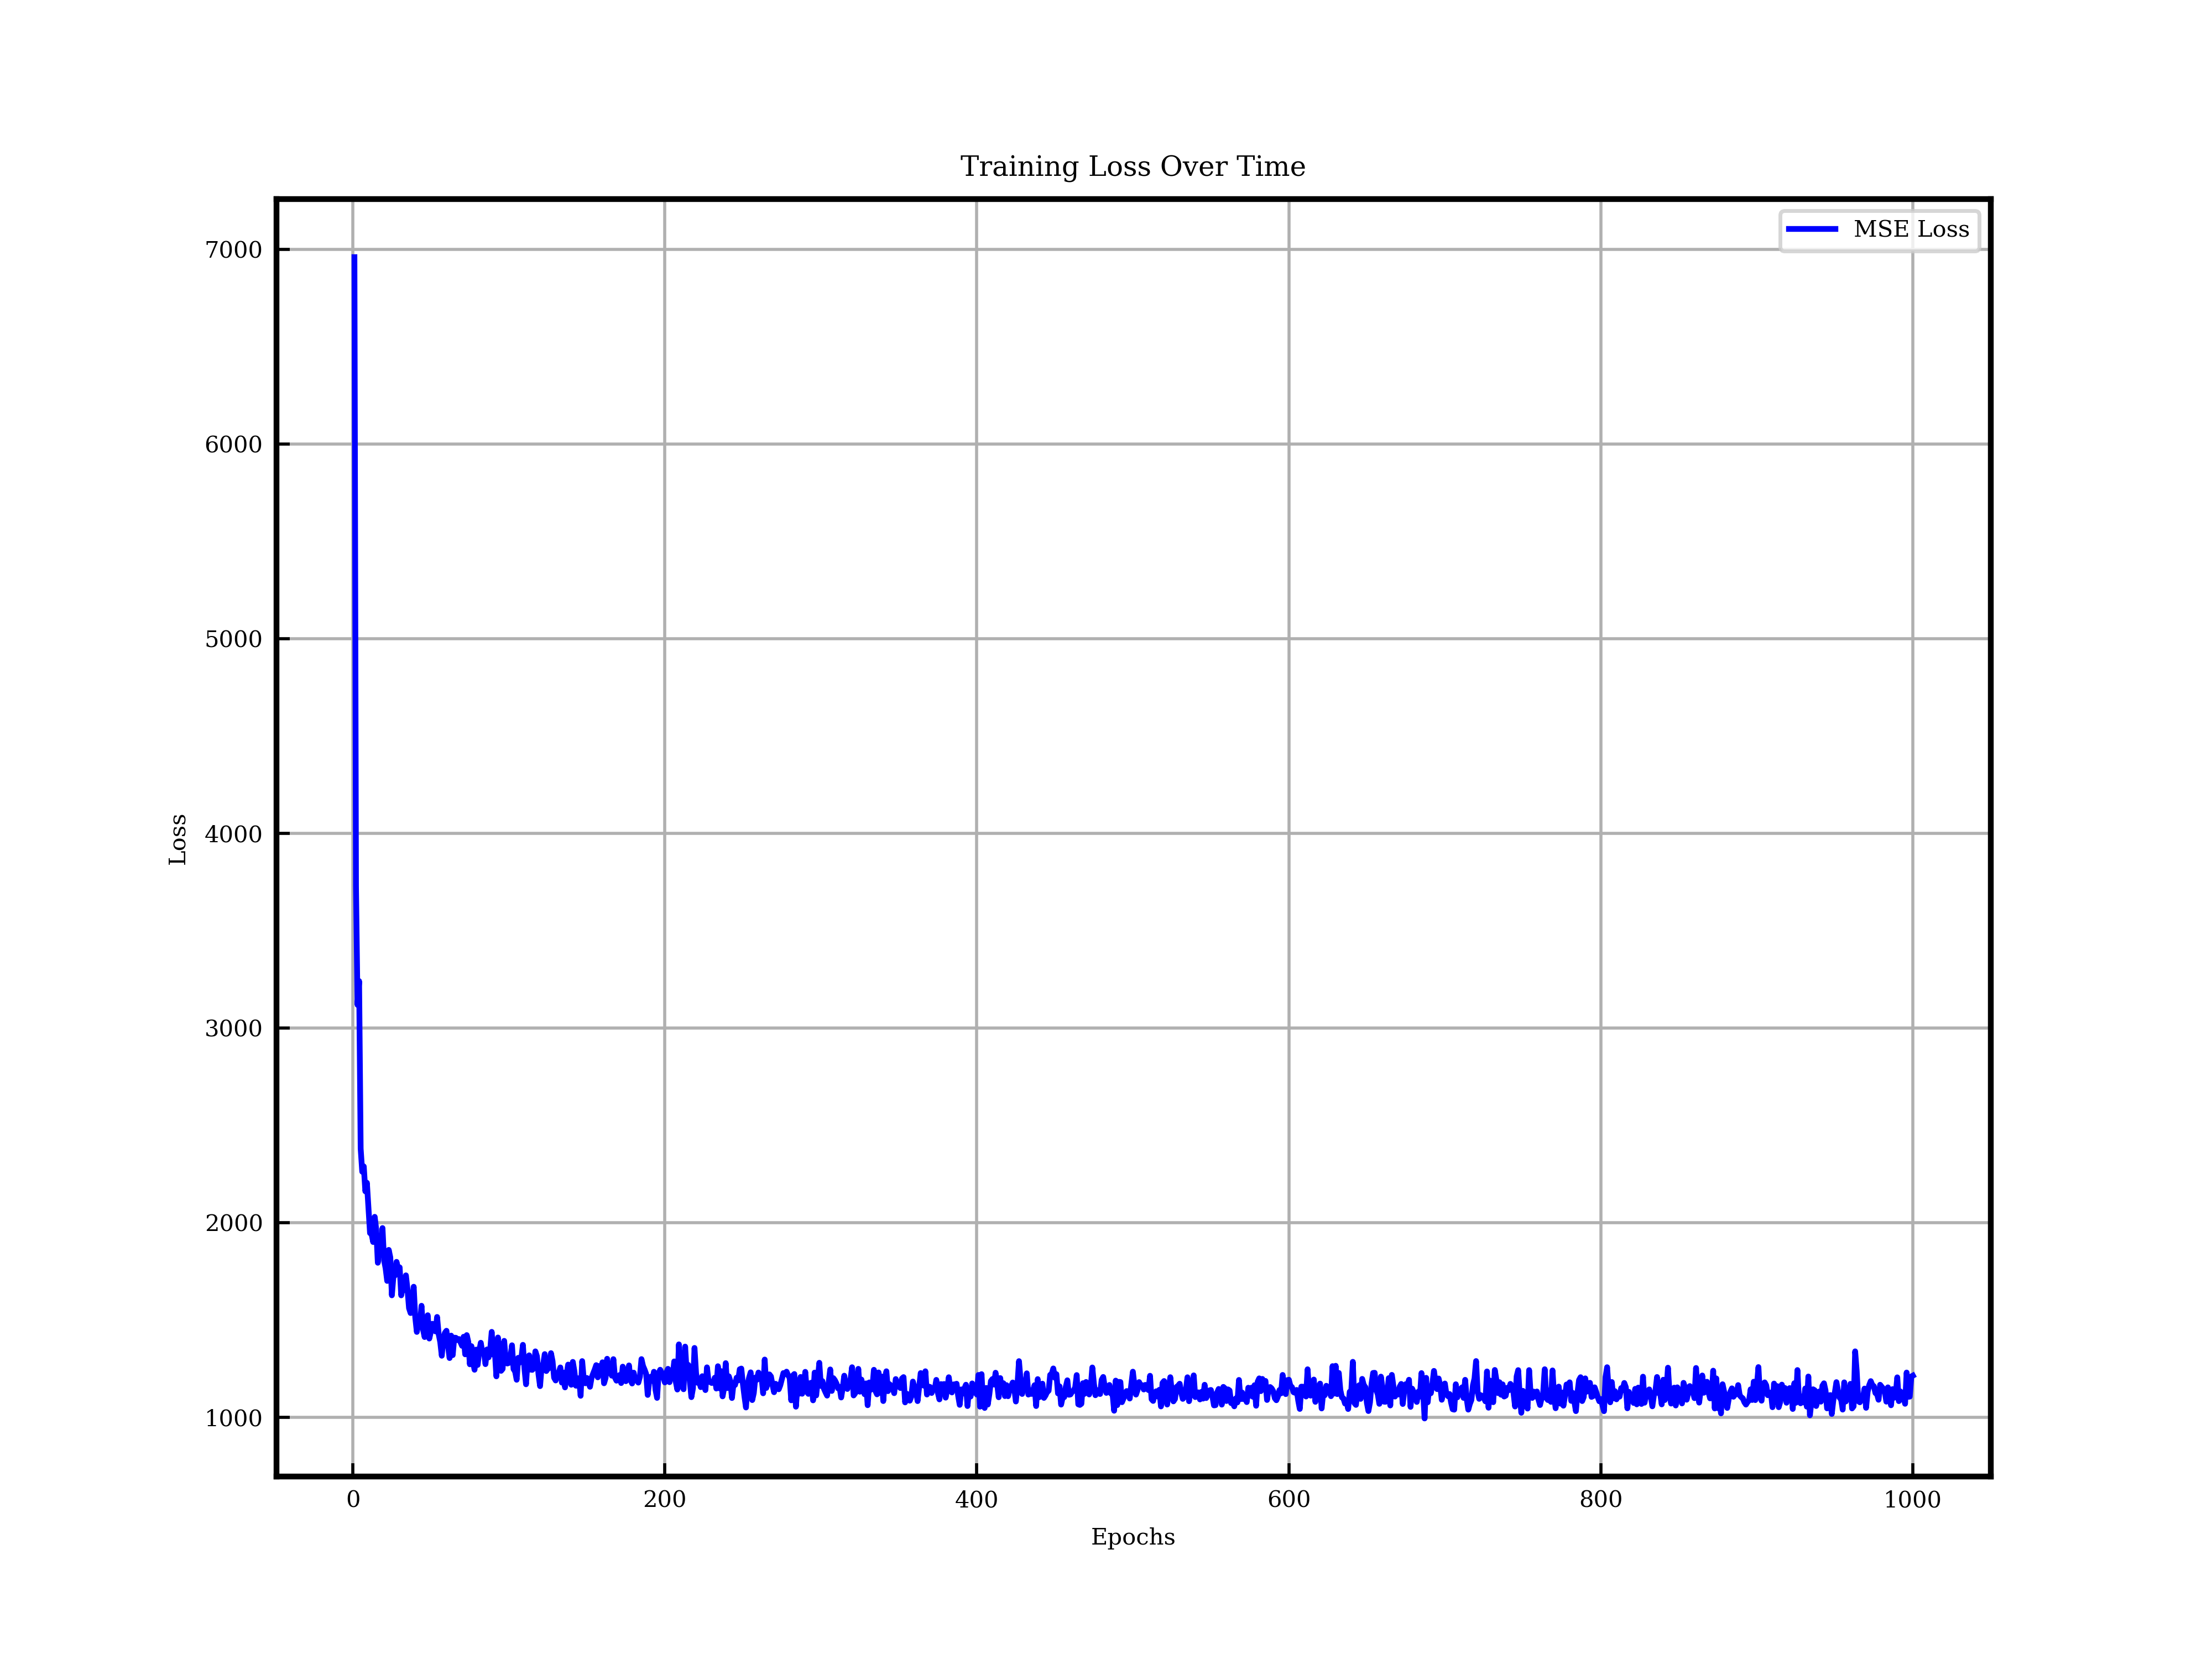
\includegraphics[width=0.75\linewidth]{figures/VAEmodels/model5/loss_plot.png}
    \caption{VAE Model 5 - MSE + KL Loss Plot}
    \label{fig:model5_loss_plot}
\end{figure}

Distributions for the values of the latent dimensions after encoding the 100,000 training shapes is presented in Figure~\ref{fig:model5_latent_dist}. Latent dimensions 1, 2, 3, 4 exhibit almost identical distributions in the Z-values, centred around 0 and resembling a normal distribution. Meanwhile, latent dimensions 5 and 6 demonstrate various peaks, with a peak emerging around -2.00, -0.75, 0.00 and 1.25 for $Z_5$. The distribution for $Z_6$ displays peaks at -1.25, 0.00, and 1.25.

\begin{figure}[H]
    \centering
    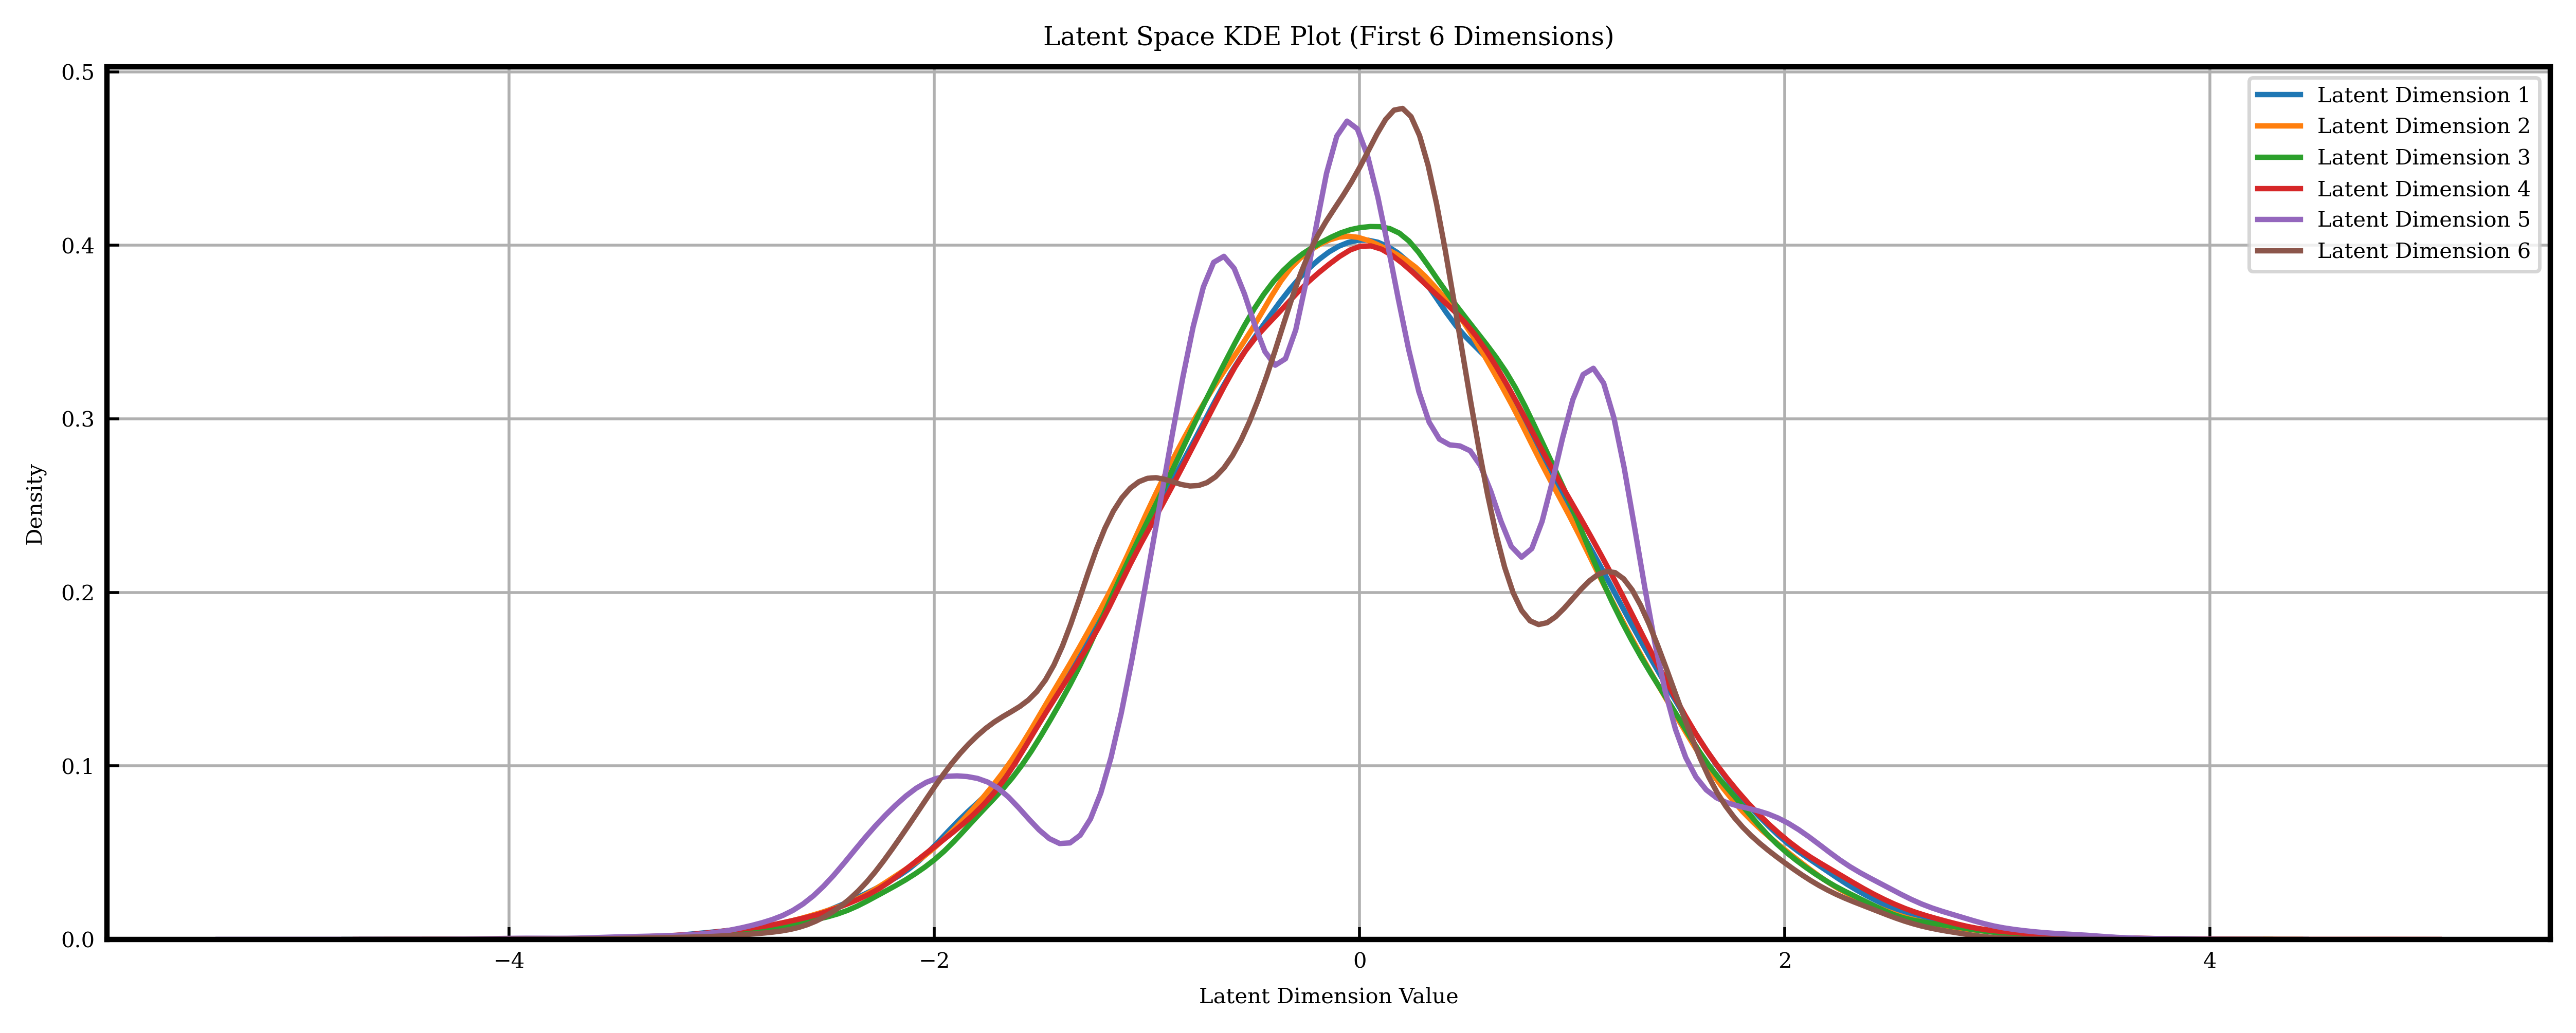
\includegraphics[width=0.75\linewidth]{figures/VAEmodels/model5/latent_distribution.png}
    \caption{Model 5 - Latent dimension distributions over all training data}
    \label{fig:model5_latent_dist}
\end{figure}

We present 4 of the configurations for latent dimensions in Figure~\ref{fig:model5_latent_visualisations} out of a total number of potential configurations of 15, though the remaining visualisations are provided in the appendix. While continuing to fix all latent dimension values to 0.0 except for those provided on the 2D visualisations, we do not observe any major change in the resultant latent space in terms of continuity or smoothness. Aligning with previous models, a single pair of latent dimensions provides the most complexity in the generated shapes over latent values between -3 and +3. This can be seen in Figure~\ref{fig:model5_z2_z3}. From the original training shapes, it can be observed that triangles, squares, diamonds, pentagons, circles, hearts and rectangles emerge with some indication of pentagons and stars, though these appear more abstract than those seen in the original training data. The largest occupancy of shapes with the lowest compactness is seen by squares in the bottom right region of Figure~\ref{fig:model5_z2_z3}, and circle like structures in the top left. Meanwhile, the highest compactness value shapes appear in more localised regions scattered across the latent space, though the physical geometries they represent appear more abstract and reflect less shapes that were provided during the VAE training phase. Figures~\ref{fig:model5_z3_z6} and \ref{fig:model5_z1_z3} demonstrate banding of shapes and associated compactness values where traversing through $Z_1$ and $Z_6$ respectively yields little variance in the generated shapes. In Figure~\ref{fig:model5_z1_z4}, we observe little change in the geometries generated, despite a change in the compactness value shown by the colour scale.

\begin{figure}[H]
  \centering

  \begin{subfigure}{0.48\textwidth}
    \centering
    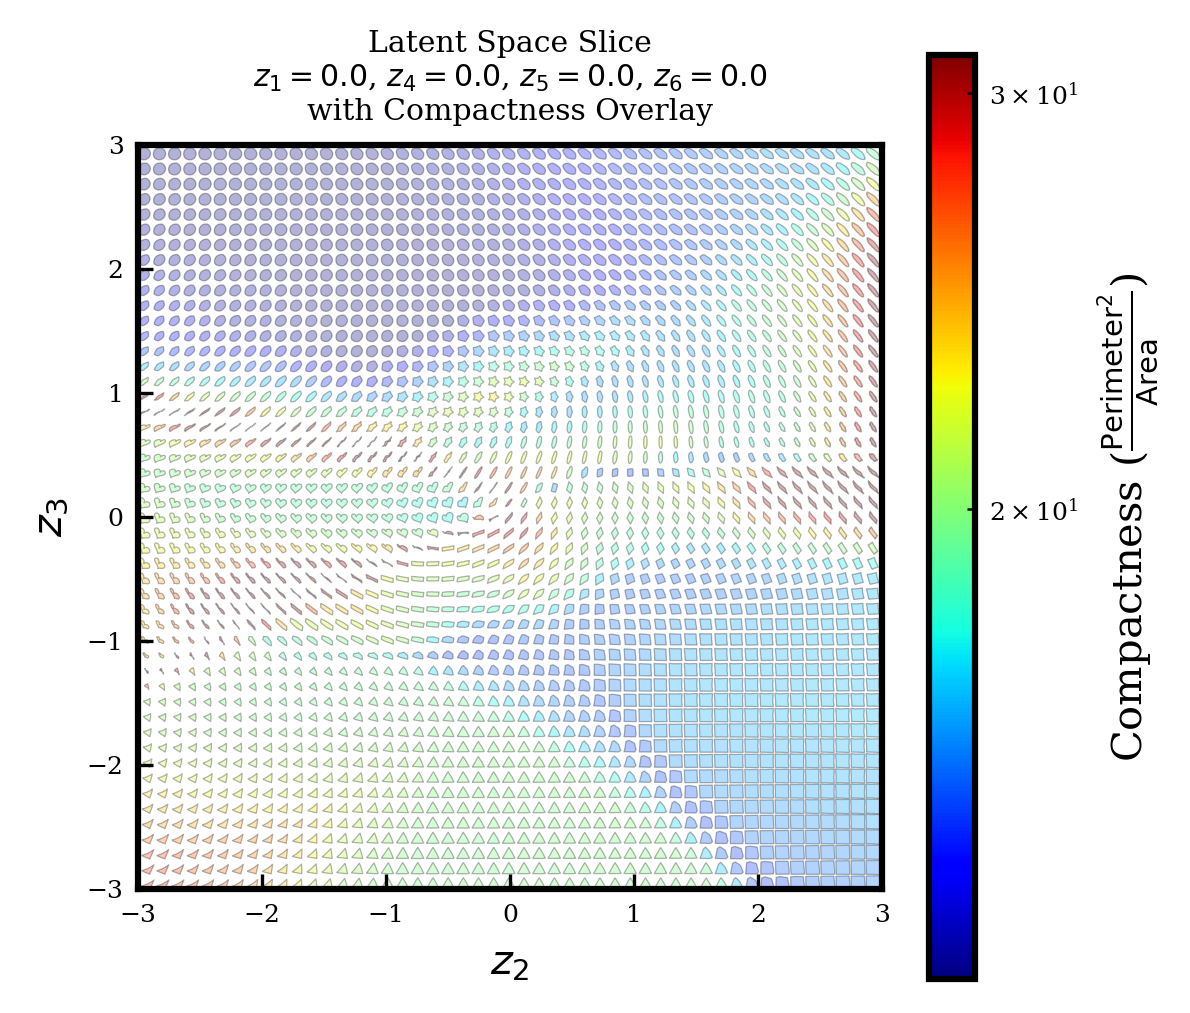
\includegraphics[width=\textwidth]{figures/VAEmodels/model5/varying_z2_z3_fixed_z1=0.0_z4=0.0_z5=0.0_z6=0.0.png}
    \caption{Latent dimensions $Z_2$ and $Z_3$}
    \label{fig:model5_z2_z3}
  \end{subfigure}
  \hfill
  \begin{subfigure}{0.48\textwidth}
    \centering
    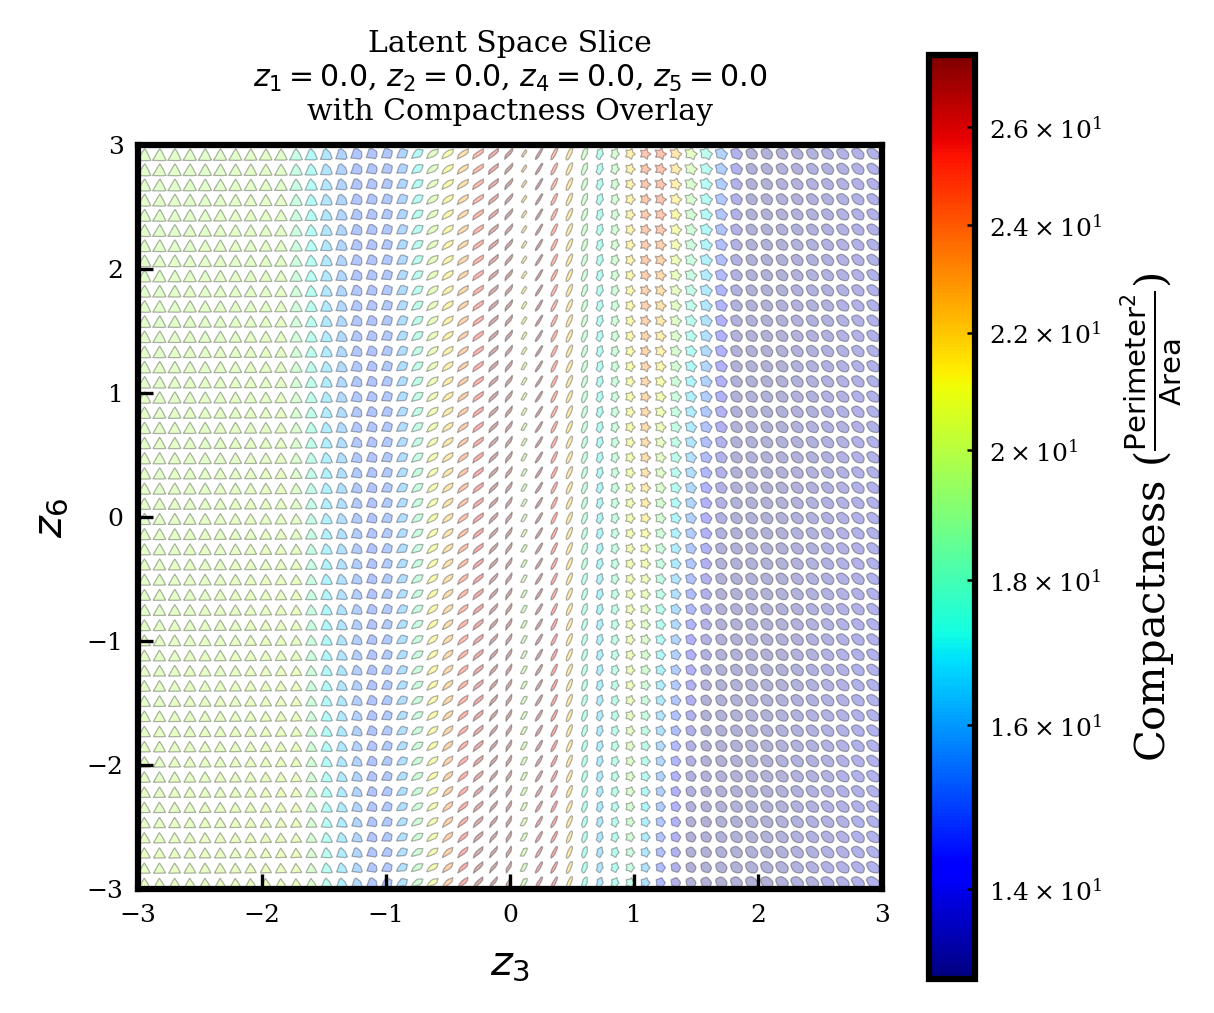
\includegraphics[width=\textwidth]{figures/VAEmodels/model5/varying_z3_z6_fixed_z1=0.0_z2=0.0_z4=0.0_z5=0.0.png}
    \caption{Latent dimensions $Z_3$ and $Z_6$}
    \label{fig:model5_z3_z6}
  \end{subfigure}

  \vspace{0.5em}

  \begin{subfigure}{0.48\textwidth}
    \centering
    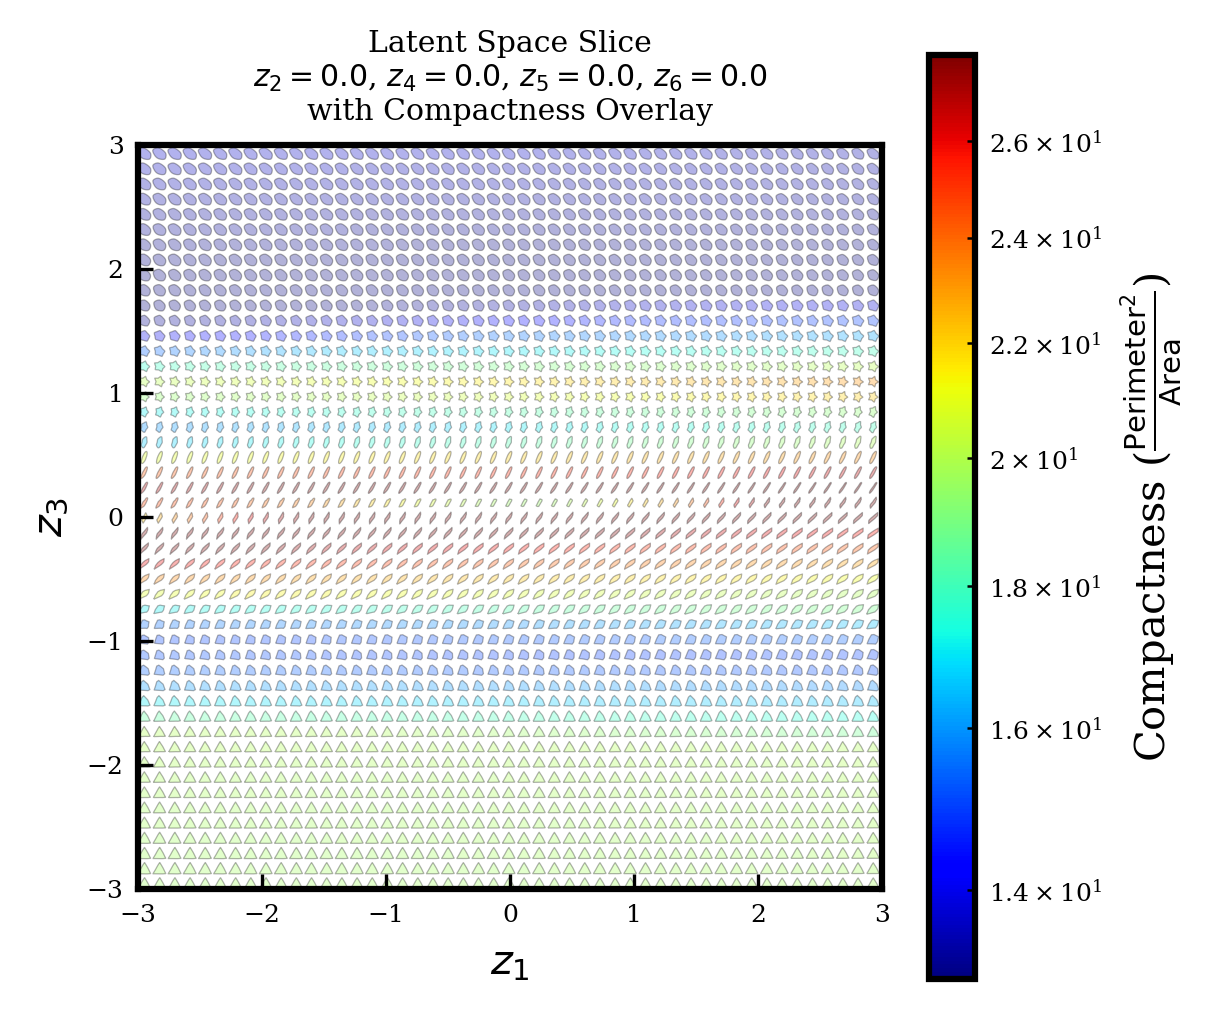
\includegraphics[width=\textwidth]{figures/VAEmodels/model5/varying_z1_z3_fixed_z2=0.0_z4=0.0_z5=0.0_z6=0.0.png}
    \caption{Latent dimensions $Z_1$ and $Z_3$}
    \label{fig:model5_z1_z3}
  \end{subfigure}
  \hfill
  \begin{subfigure}{0.48\textwidth}
    \centering
    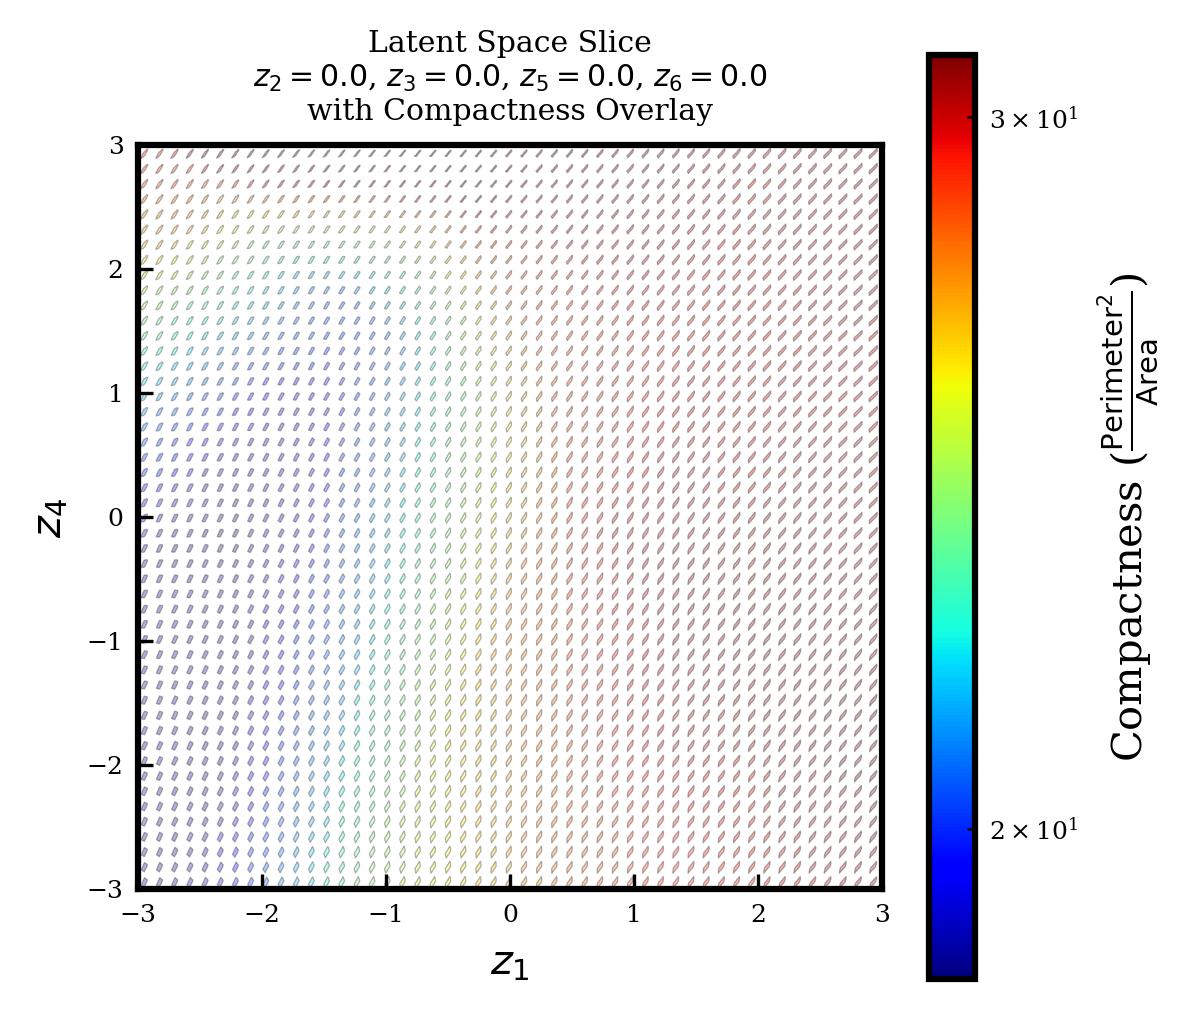
\includegraphics[width=\textwidth]{figures/VAEmodels/model5/varying_z1_z4_fixed_z2=0.0_z3=0.0_z5=0.0_z6=0.0.png}
    \caption{Latent dimensions $Z_1$ and $Z_4$}
    \label{fig:model5_z1_z4}
  \end{subfigure}

  \caption{Model 5 - Latent space visualisation with compactness colourmap.}
  \label{fig:model5_latent_visualisations}
\end{figure}


\subsection{Genetic Algorithm}
To demonstrate the effect of transforming design problems into a low-dimensional latent representation prior to performing optimisation, we first demonstrate the capability of a genetic algorithm to optimise for the geometric compactness metric (Equation~\eqref{eq:compactness}) for high-dimensional, random noise shapes defined by a series of nodes of fixed connectivity as described in Section~\ref{Geometry}. While the end use-case, and as is demonstrated in this research, is to explore designs that reflect realistic samples, we will first approach the problem of random noise, an arguably more complex geometric challenge and starting condition to solve for. Examples of such starting representations are shown in Figure~\ref{fig:random_noise_ga_shapes}. We begin with an initial resolution (i.e, nodes defining the random polygons) of 10 and apply the genetic algorithm on polygons up to resolution of 300 nodes (see Table~\ref{tab:GA_models_original}). Despite the shapes being represented on a 2D manifold, the dimensionality of the design problem and hence the design space is defined by the number of varying parameters, or number of geometric nodes in the case of this research and it is expected that as we move towards increasing resolutions, the effectiveness of the GA to optimise for compactness will deteriorate. After motivating the necessity to explore more efficient design-space representations, we proceed to perform optimisation via the genetic algorithm directly in the latent space, whereby the genes of the individuals are represented by the latent values of the latent vectors for each $L$-dimensional latent representation starting from $L=2$ up to $L=6$. In contrast to the 200-node representation, this yields a significant reduction in the dimensionality of the design space.

\subsubsection{Genetic Algorithm - Random Polygon Results}\label{random_polygon_ga}
The following section presents the initial starting population of random polygons and samples of the final population after 1000 generations of the genetic algorithm for each of the GAs lsted in Table~\ref{tab:GA_models_original}.

\subsubsection*{GA1 - Random Noise Polygon: Resolution = 10; Number of Parents = 4; Initial Population = 100}

In Figure~\ref{fig:GA1_before_after_GA}, we present a sample of the initial population of random noise shapes, defined by 10 nodes in 2D. The genetic algorithm, GA1, is applied to an initial population of 100 and evolved for 1000 generations to these random noise shapes. Figure~\ref{fig:GA1_final} shows a sample of the resultant shapes after the 1000th generation. The sample demonstrates the GA has iterated towards circular-like geometries, only limited by the resolution of 10 not permitting smooth sided circles. The fitness curve in Figure~\ref{fig:GA1_fitness_curve} displays a maximum fitness value of ~0.075, which is defined as the inverse of the compactness metric - this maximum is reached after 100 generations of GA evolution. Shapes with higher fitness values will tend towards circles, if defined by a suitably high number of nodes. 

\begin{figure}[H]
    \centering
    \begin{subfigure}[b]{0.45\textwidth}
        \centering
        \includegraphics[width=\textwidth]{figures/GAResults/GA1/10point_initial_pop.png}
        \caption{Initial starting population}
        \label{fig:GA1_starting}
    \end{subfigure}
    \hfill
    \begin{subfigure}[b]{0.45\textwidth}
        \centering
        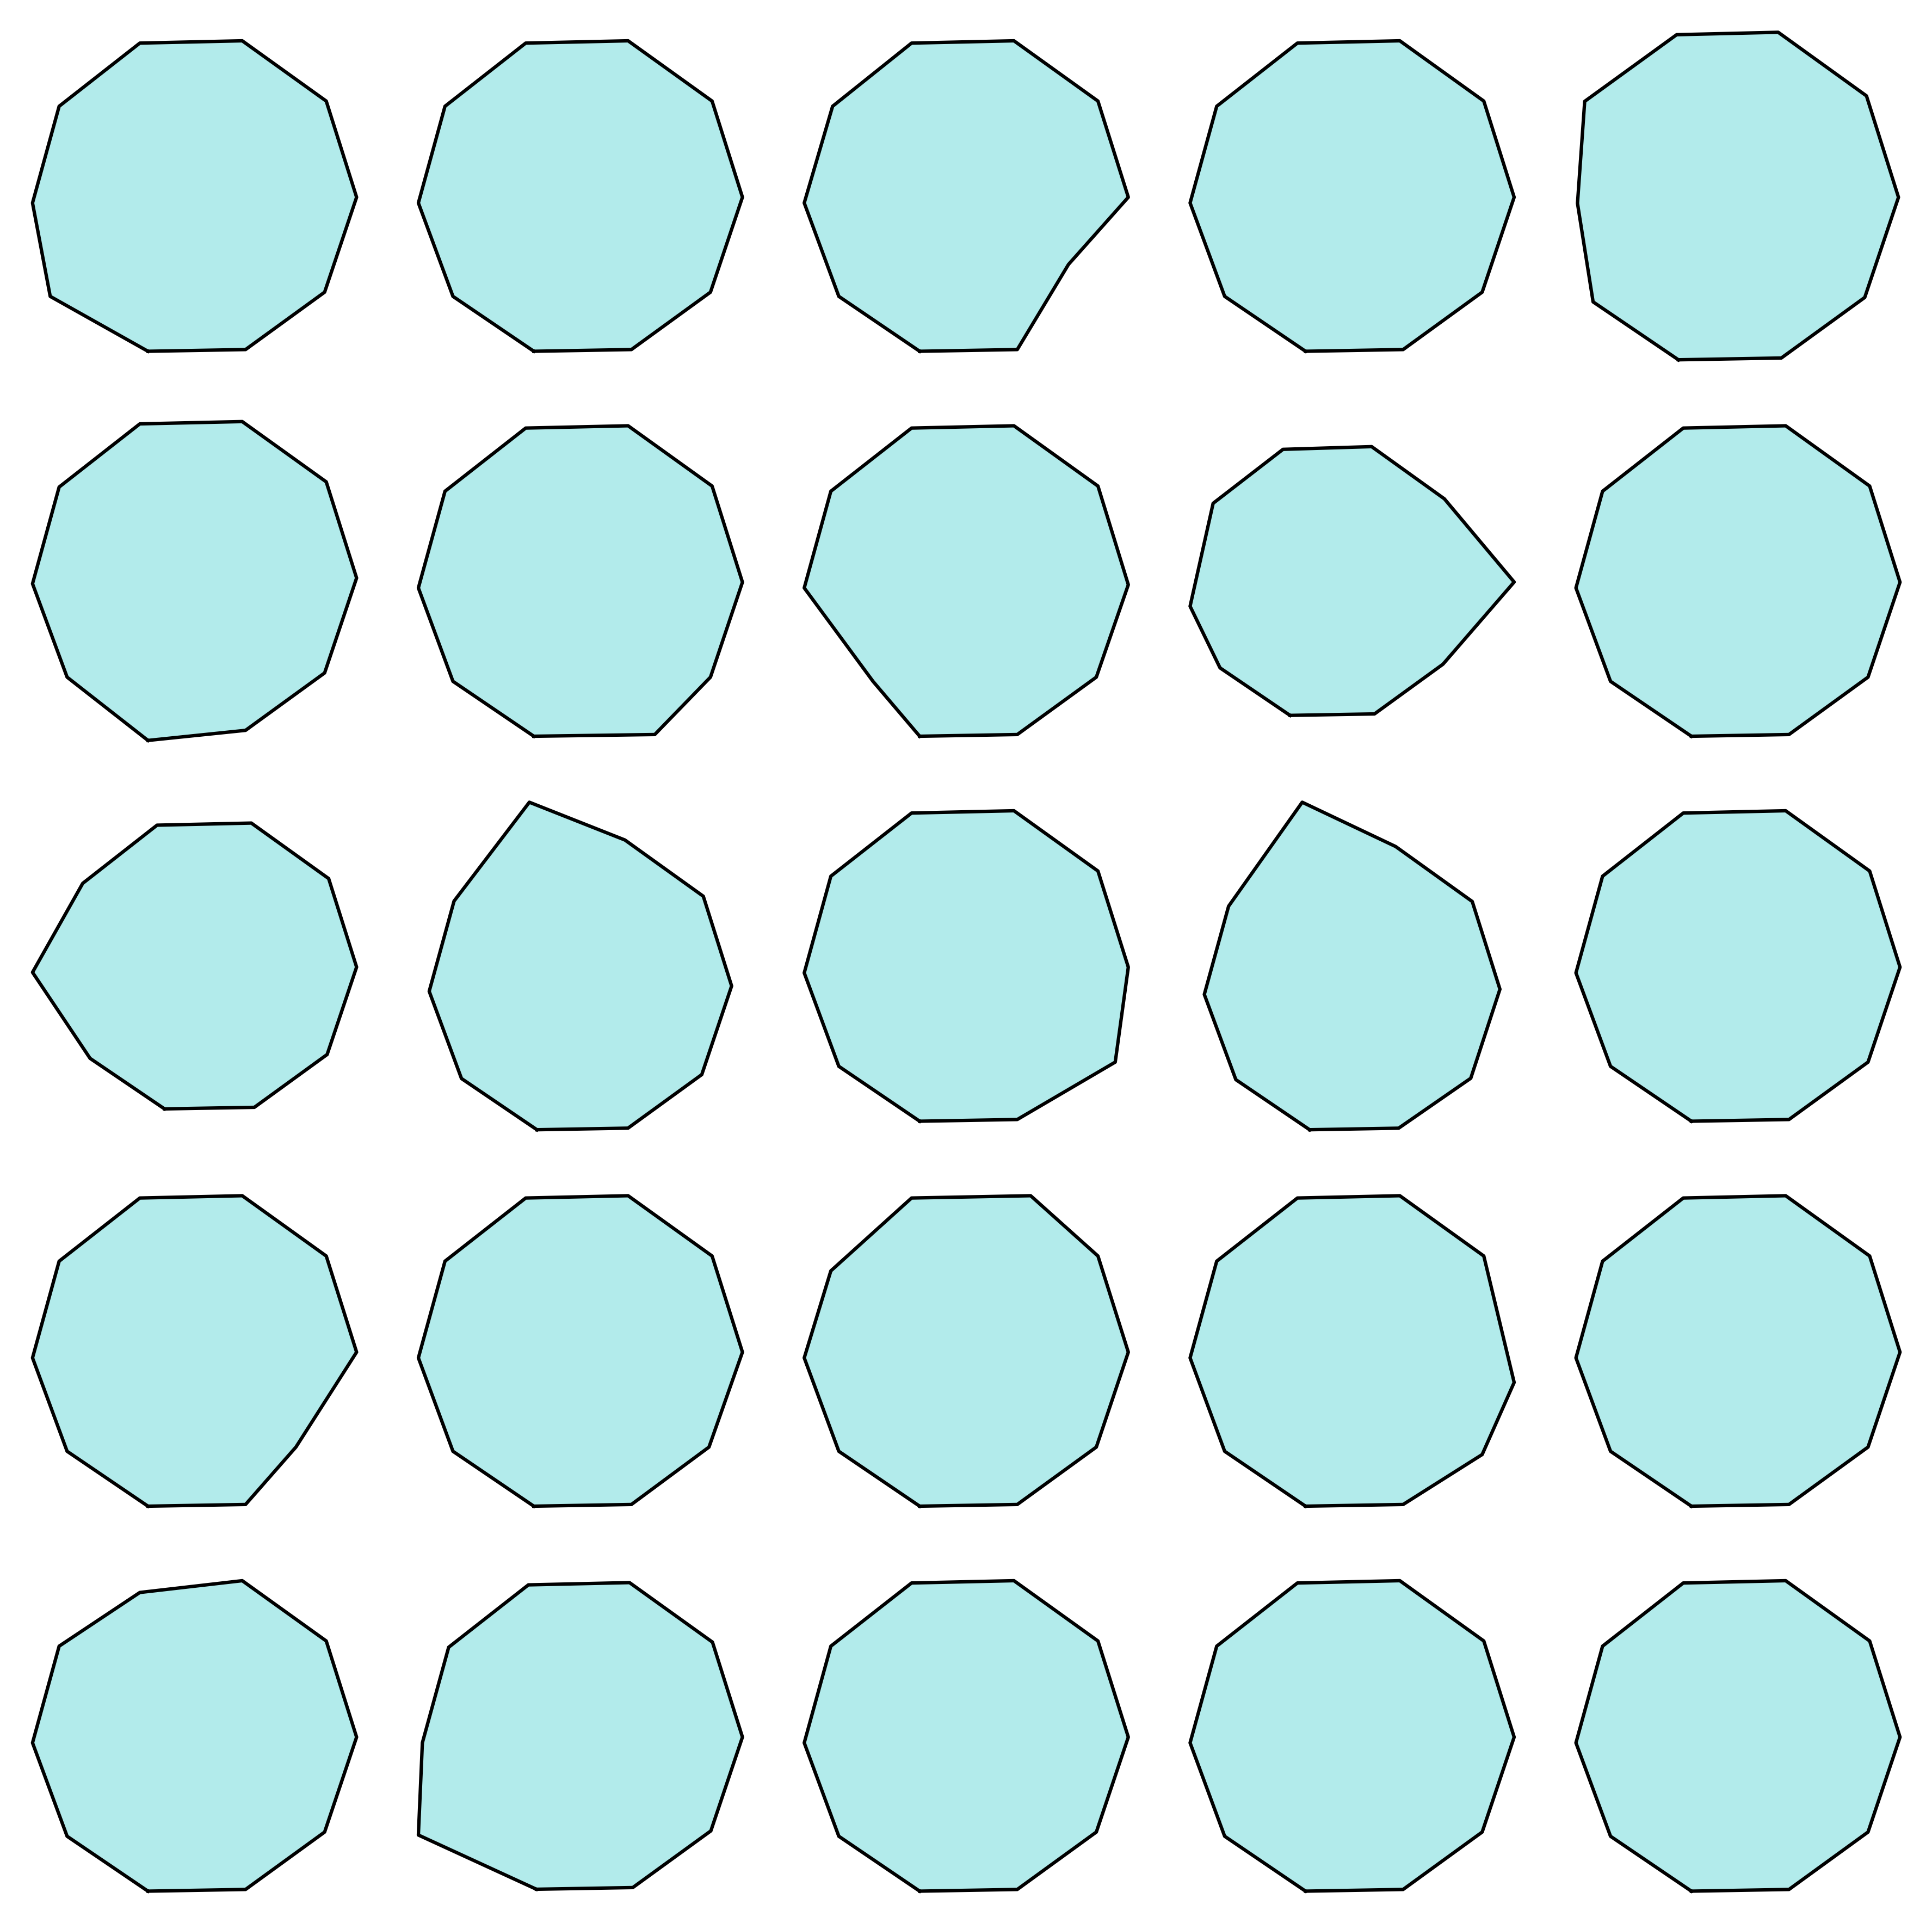
\includegraphics[width=\textwidth]{figures/GAResults/GA1/final_population.png}
        \caption{After 1000 generations of GA evolution.}
        \label{fig:GA1_final}
    \end{subfigure}
    \caption{GA1 starting and final population after optimising for compactness metric.}
    \label{fig:GA1_before_after_GA}
\end{figure}

\begin{figure}[H]
    \centering
    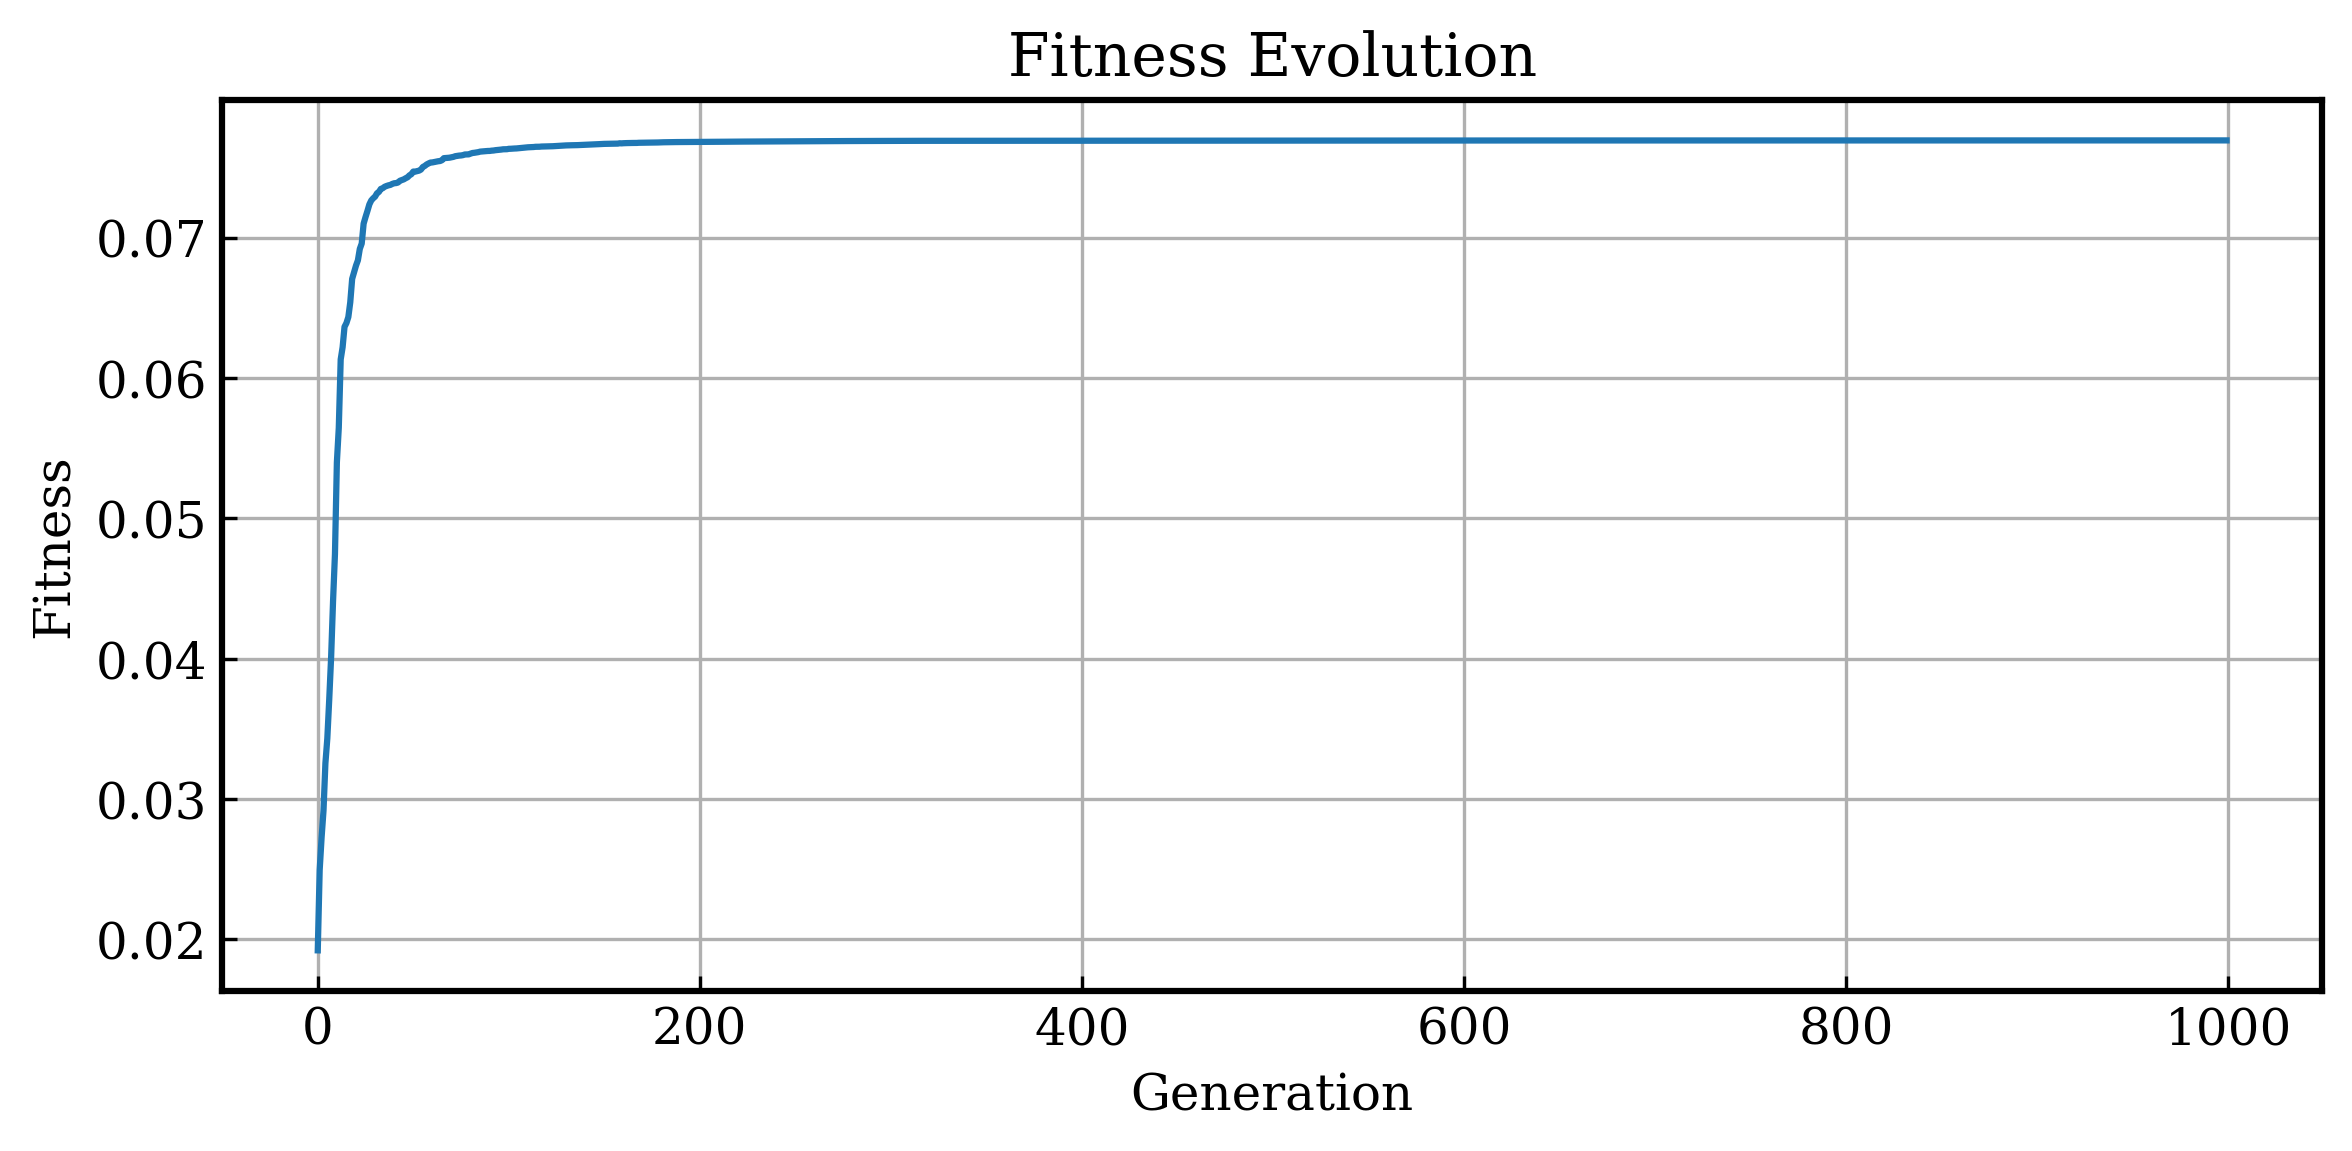
\includegraphics[width=0.75\linewidth]{figures/GAResults/GA1/1000gens_4pars_100initpop_5pcent_mut.png}
    \caption{GA1 Genetic Algorithm Fitness Score Evolution}
    \label{fig:GA1_fitness_curve}
\end{figure}

\subsubsection*{GA2 - Random Noise Polygon: Resolution = 10; Number of Parents = 10; Initial Population = 100}

Similarly, in Figure~\ref{fig:GA2_before_after_GA} for GA2, we increase the number of parents used during each evolution to 10 from 4 to increase the diversity of shapes that are considered for mutation and crossover at each evolution. The resolution and initial population size is maintained. A similar result is seen, with circular like shapes realised after 1000 generations, and a fitness value of ~0.075, though occurring after 50 generations as seen in Figure~\ref{fig:GA2_fitness}

\begin{figure}[H]
    \centering
    \begin{subfigure}[b]{0.45\textwidth}
        \centering
        \includegraphics[width=\textwidth]{figures/GAResults/GA2/10point_initial_pop.png}
        \caption{Initial starting population}
        \label{fig:GA2_starting}
    \end{subfigure}
    \hfill
    \begin{subfigure}[b]{0.45\textwidth}
        \centering
        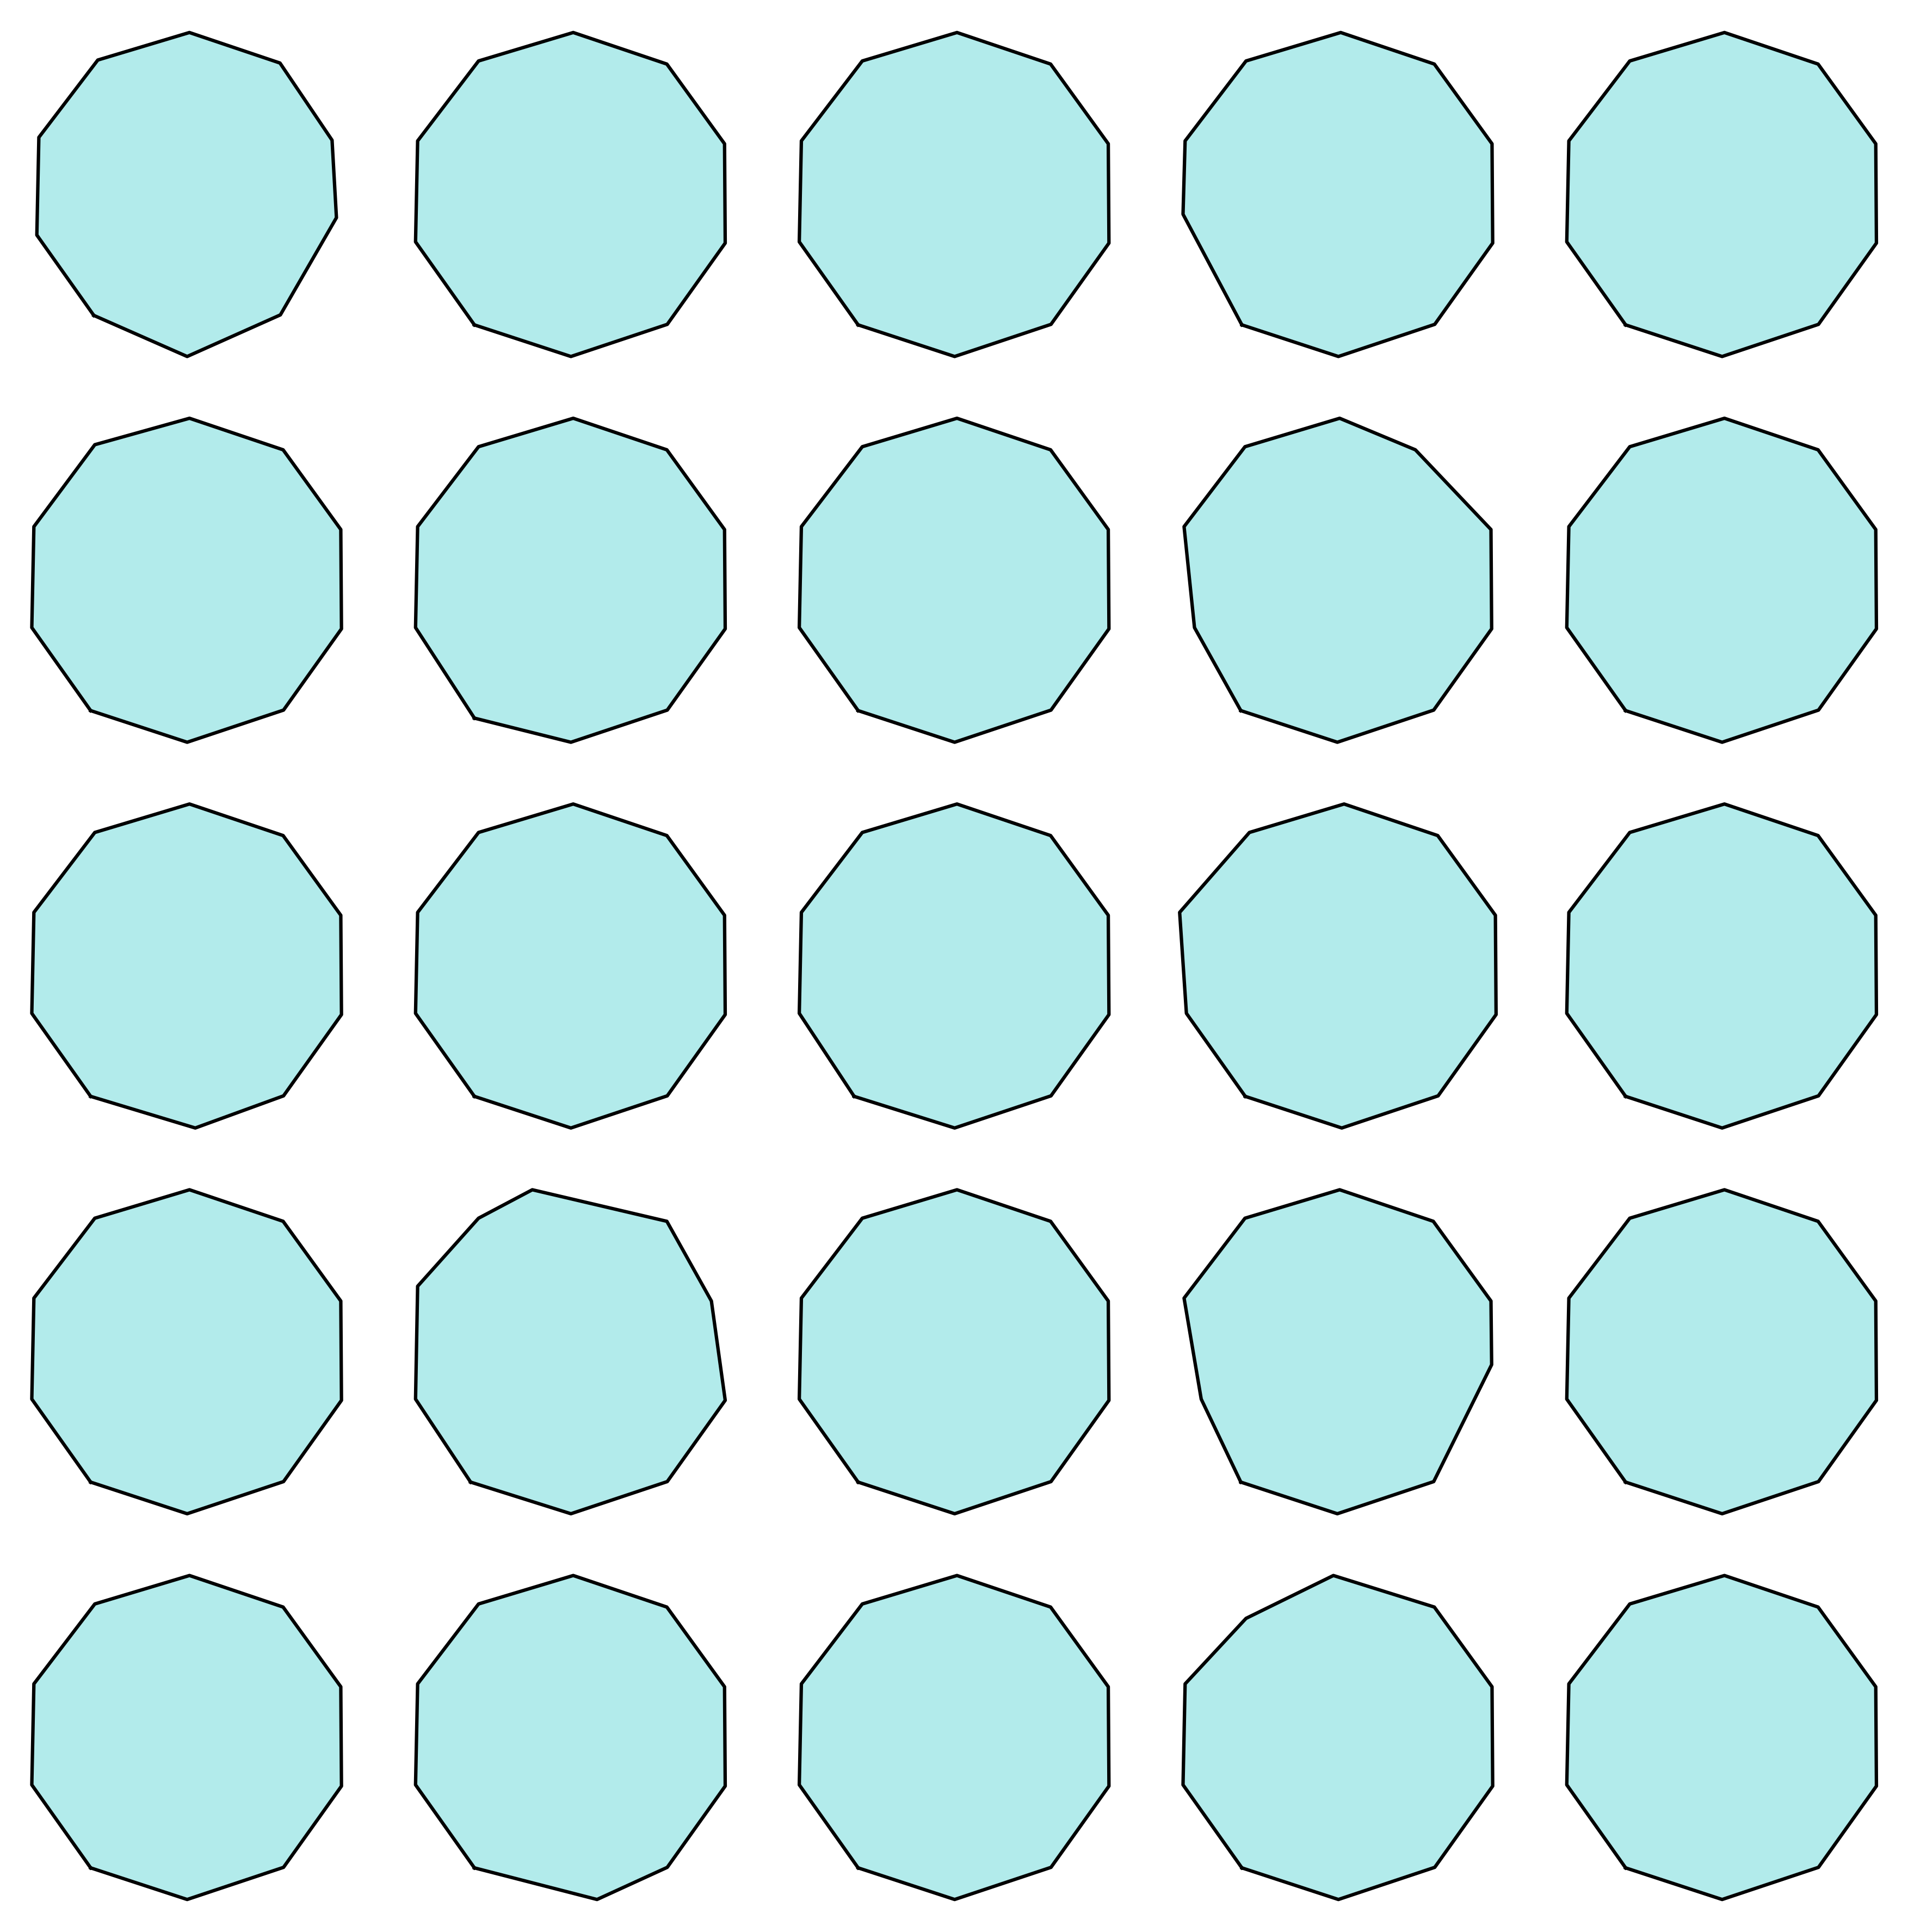
\includegraphics[width=\textwidth]{figures/GAResults/GA2/final_population.png}
        \caption{After 1000 generations of GA evolution.}
        \label{fig:GA2_final}
    \end{subfigure}
    \caption{GA2 starting and final population after optimising for compactness metric.}
    \label{fig:GA2_before_after_GA}
\end{figure}

\begin{figure}[H]
    \centering
    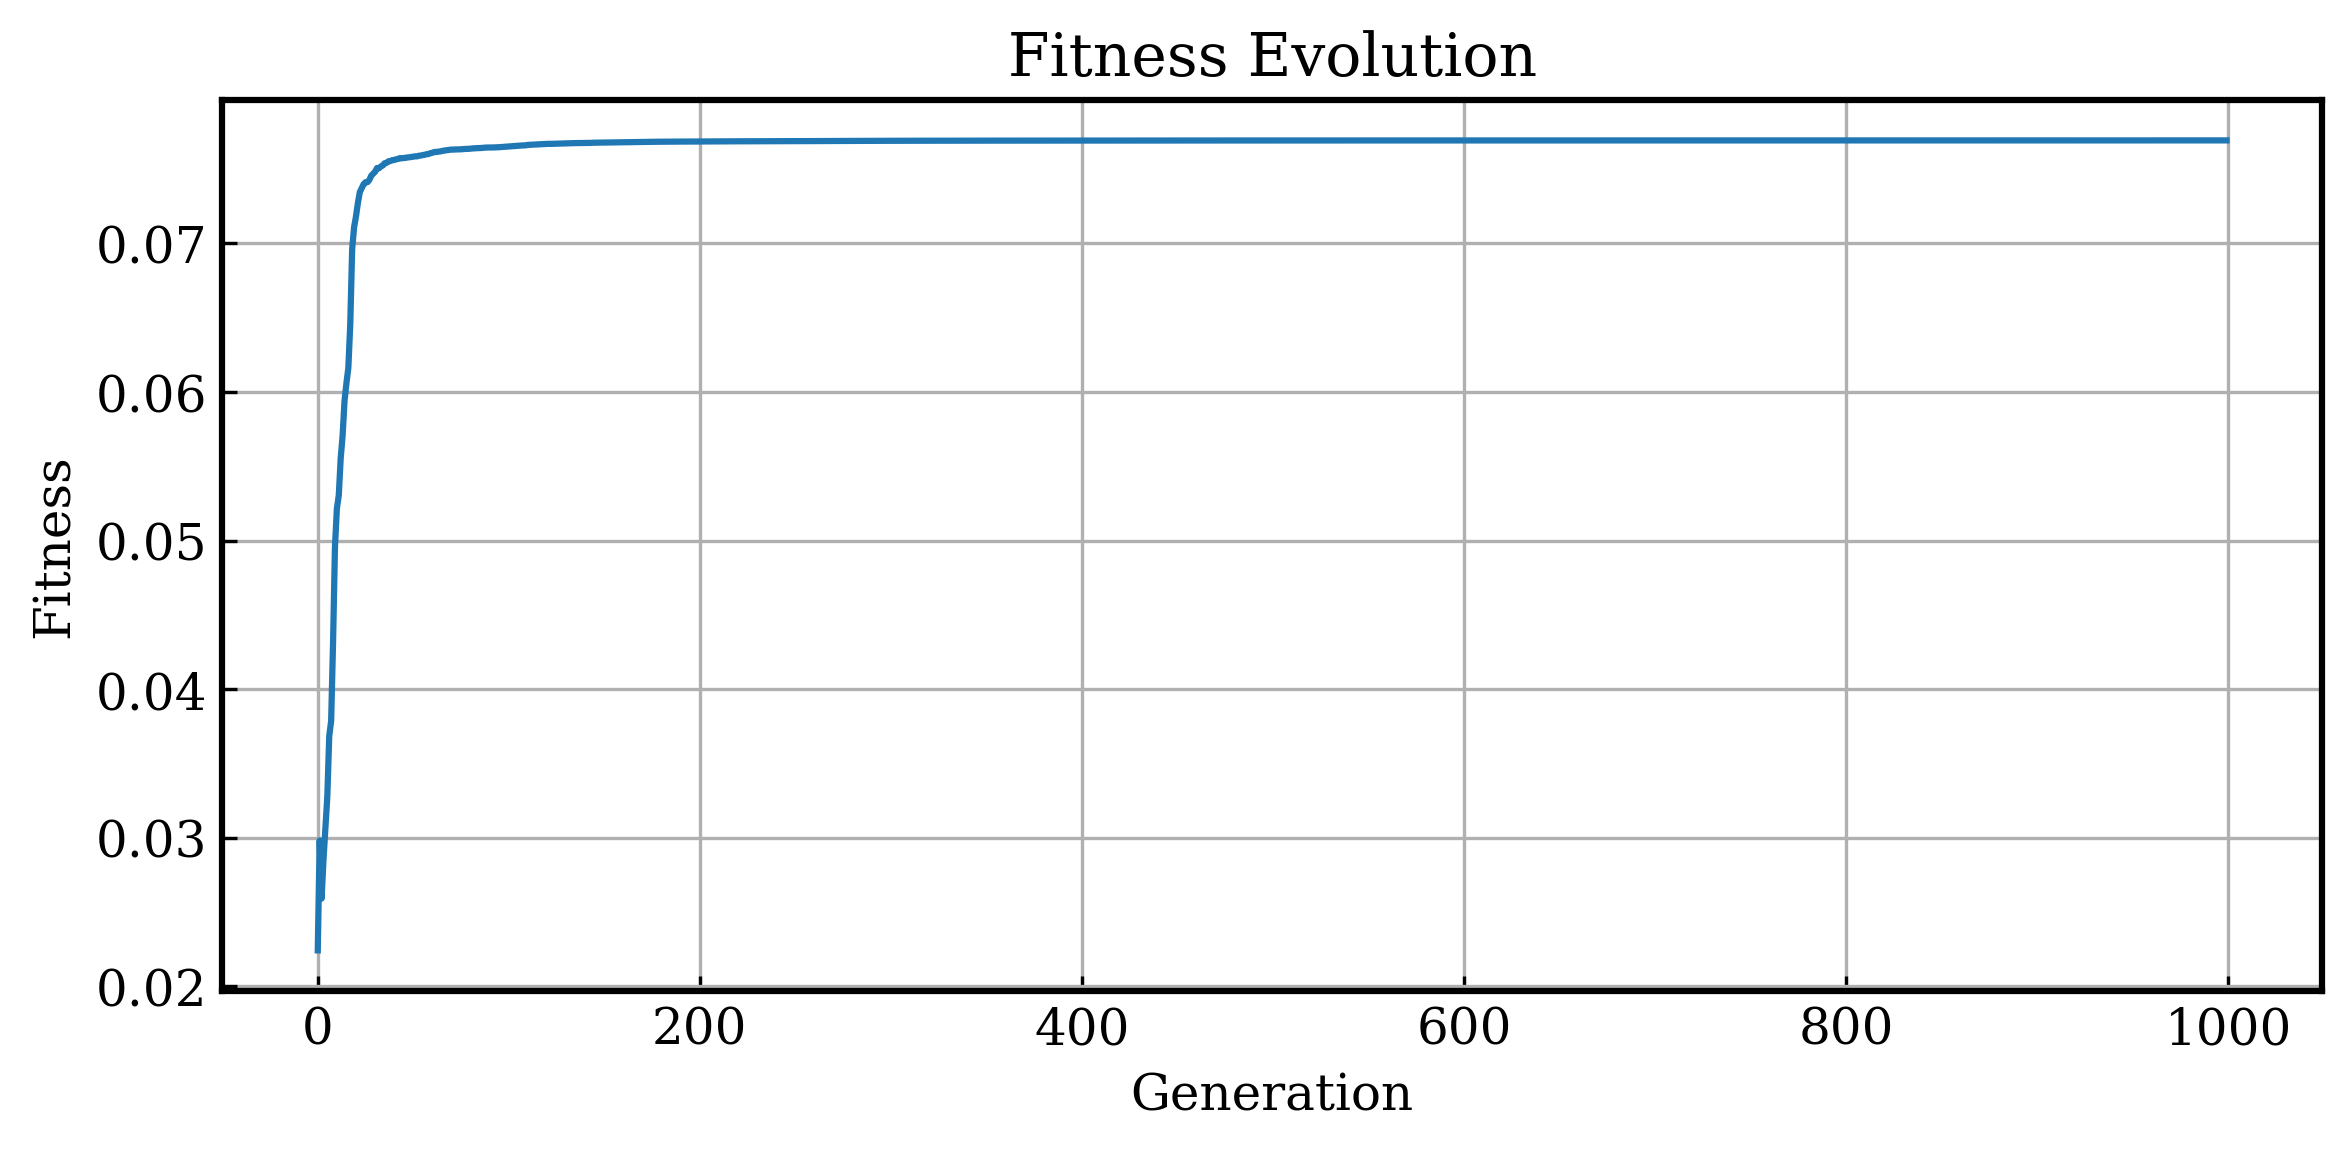
\includegraphics[width=0.75\linewidth]{figures/GAResults/GA2/1000gens_10pars_100initpop_5pcent_mut.png}
    \caption{GA2 Genetic Algorithm Fitness Score Evolution}
    \label{fig:GA2_fitness}
\end{figure}



\subsubsection*{GA3 - Random Noise Polygon: Resolution = 30; Number of Parents = 10; Initial Population = 100}
GA3 further increases the resolution of the initial population, with a total of 30 nodes defining the geometries. Figure~\ref{fig:GA3_before_after_GA} shows samples of the the initial and final population afte 100 evolutions, with Figure~\ref{fig:GA3_fitness} showing a final fitness value of 0.075, but being achieved after later evolutions (~800).
\begin{figure}[H]
    \centering
    \begin{subfigure}[b]{0.45\textwidth}
        \centering
        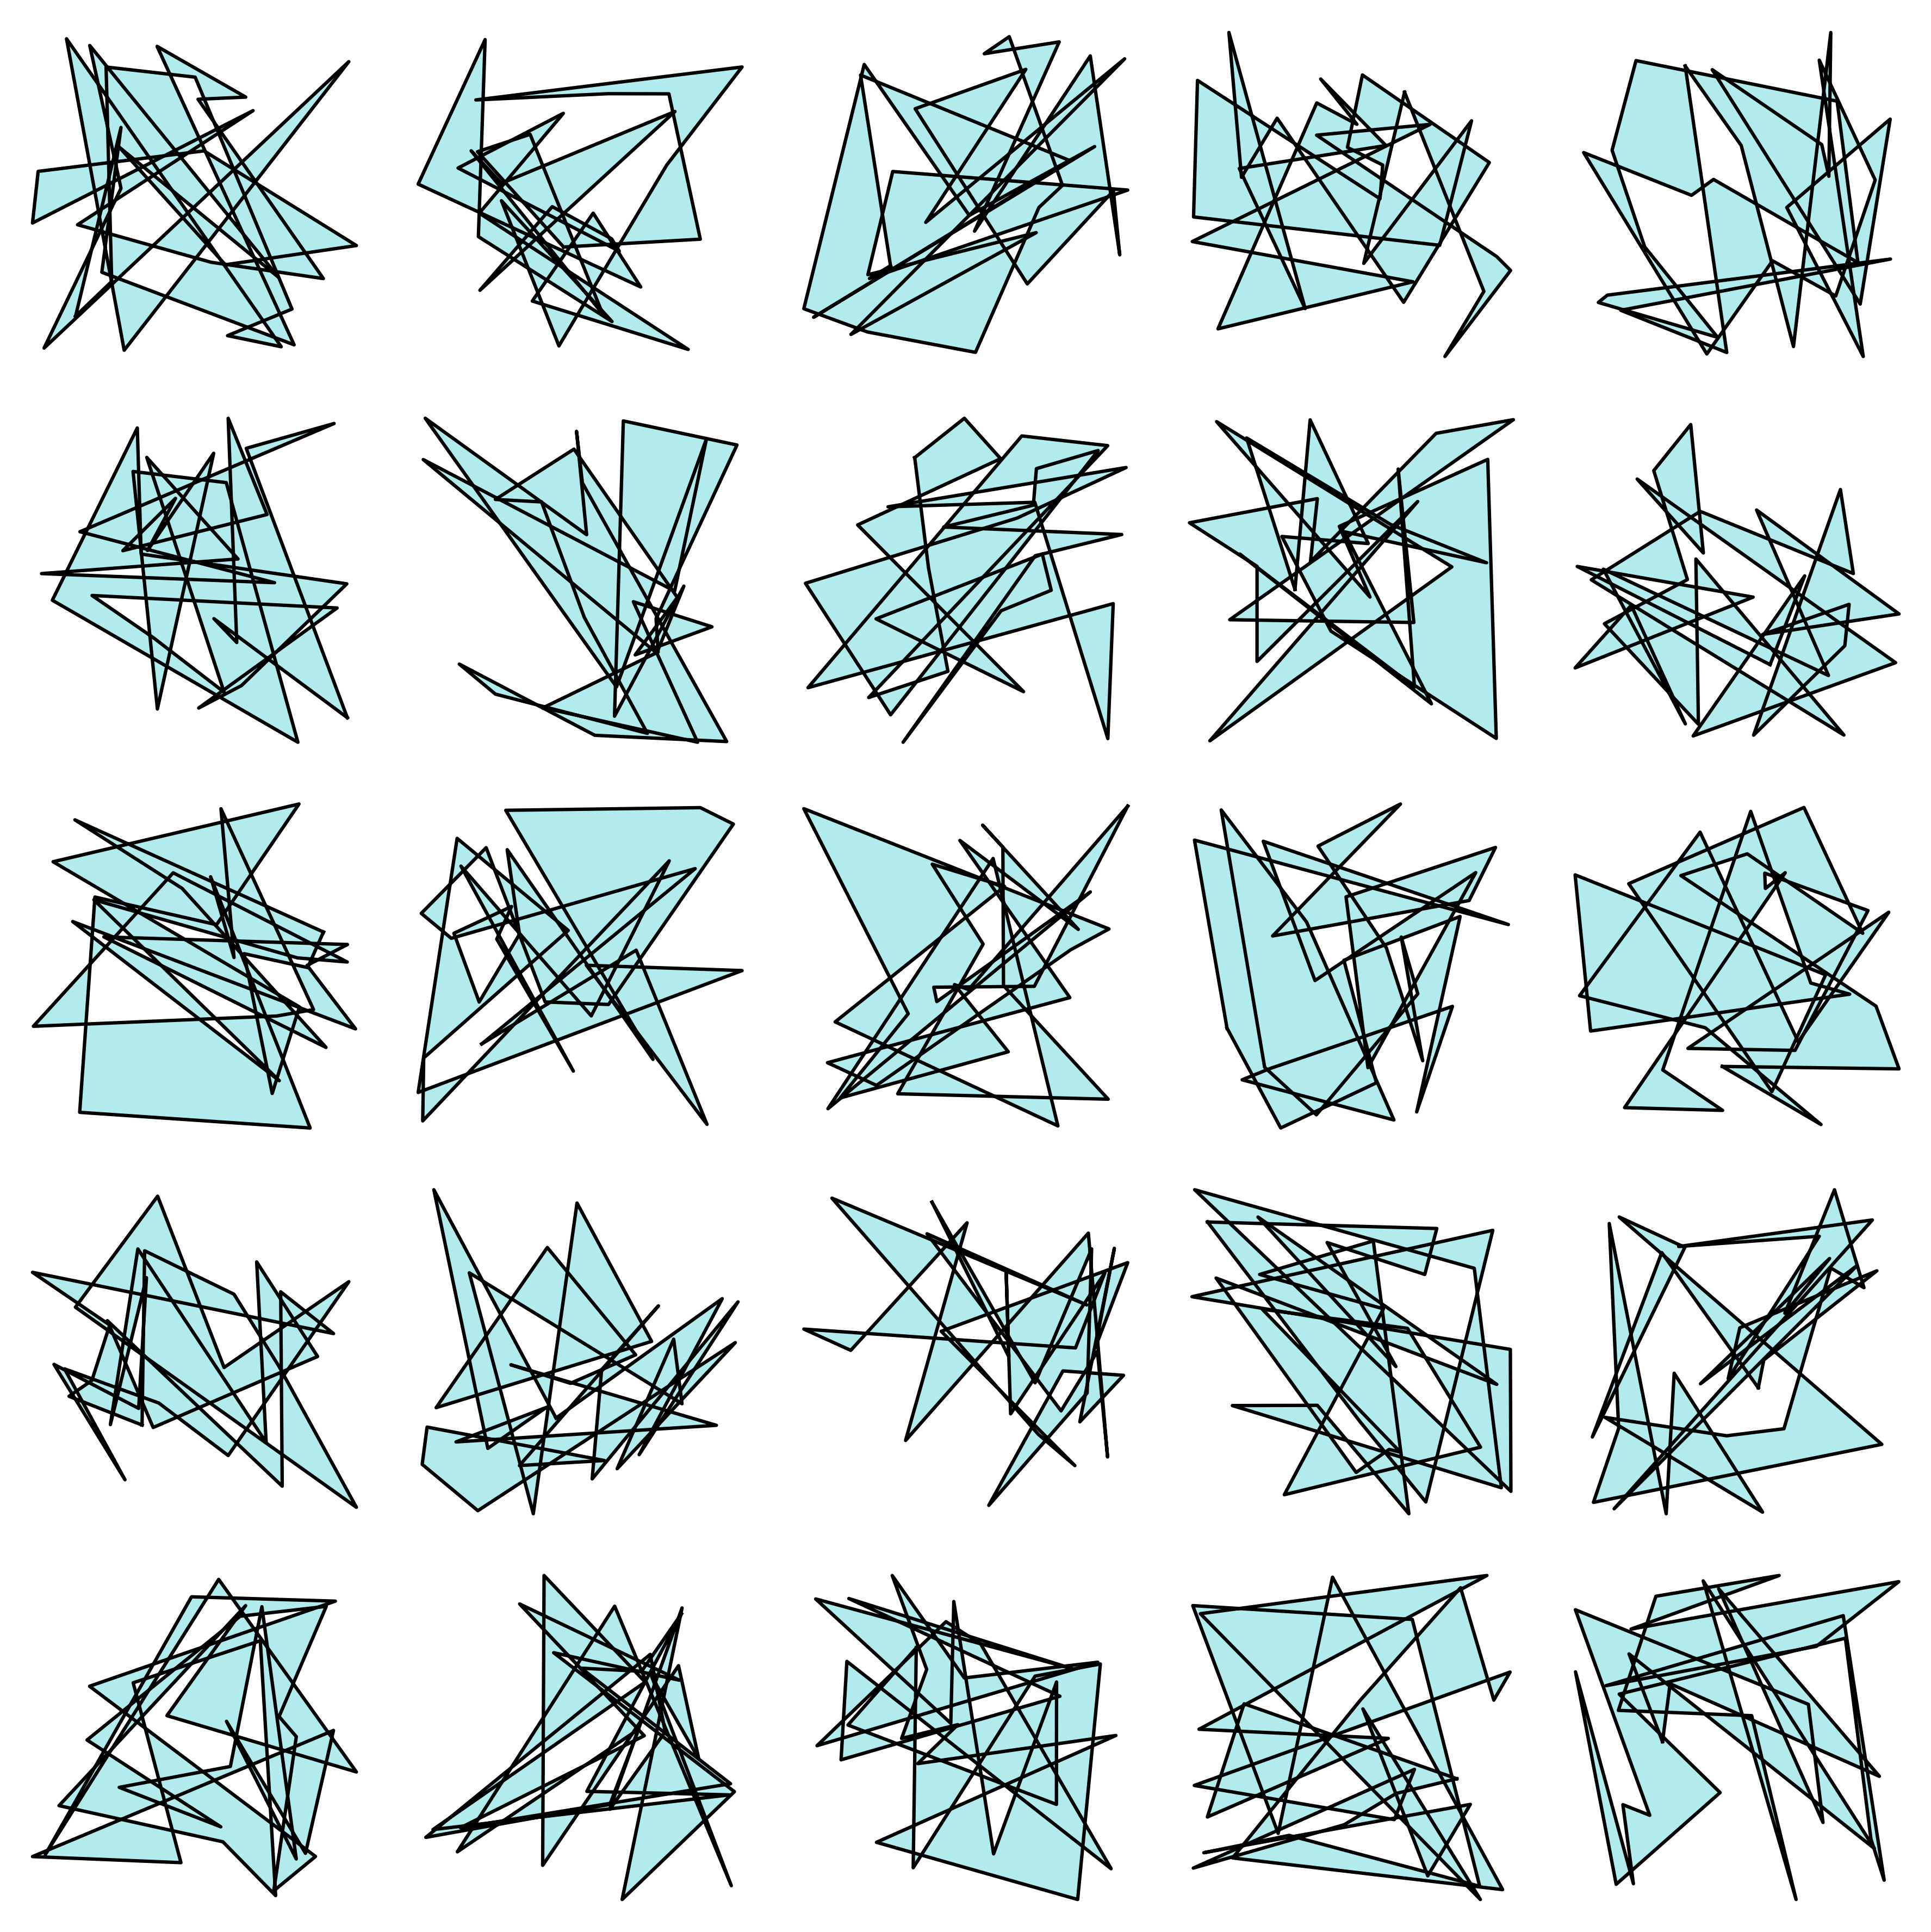
\includegraphics[width=\textwidth]{figures/GAResults/GA3/30point_initial_pop.png}
        \caption{Initial starting population}
        \label{fig:GA3_starting}
    \end{subfigure}
    \hfill
    \begin{subfigure}[b]{0.45\textwidth}
        \centering
        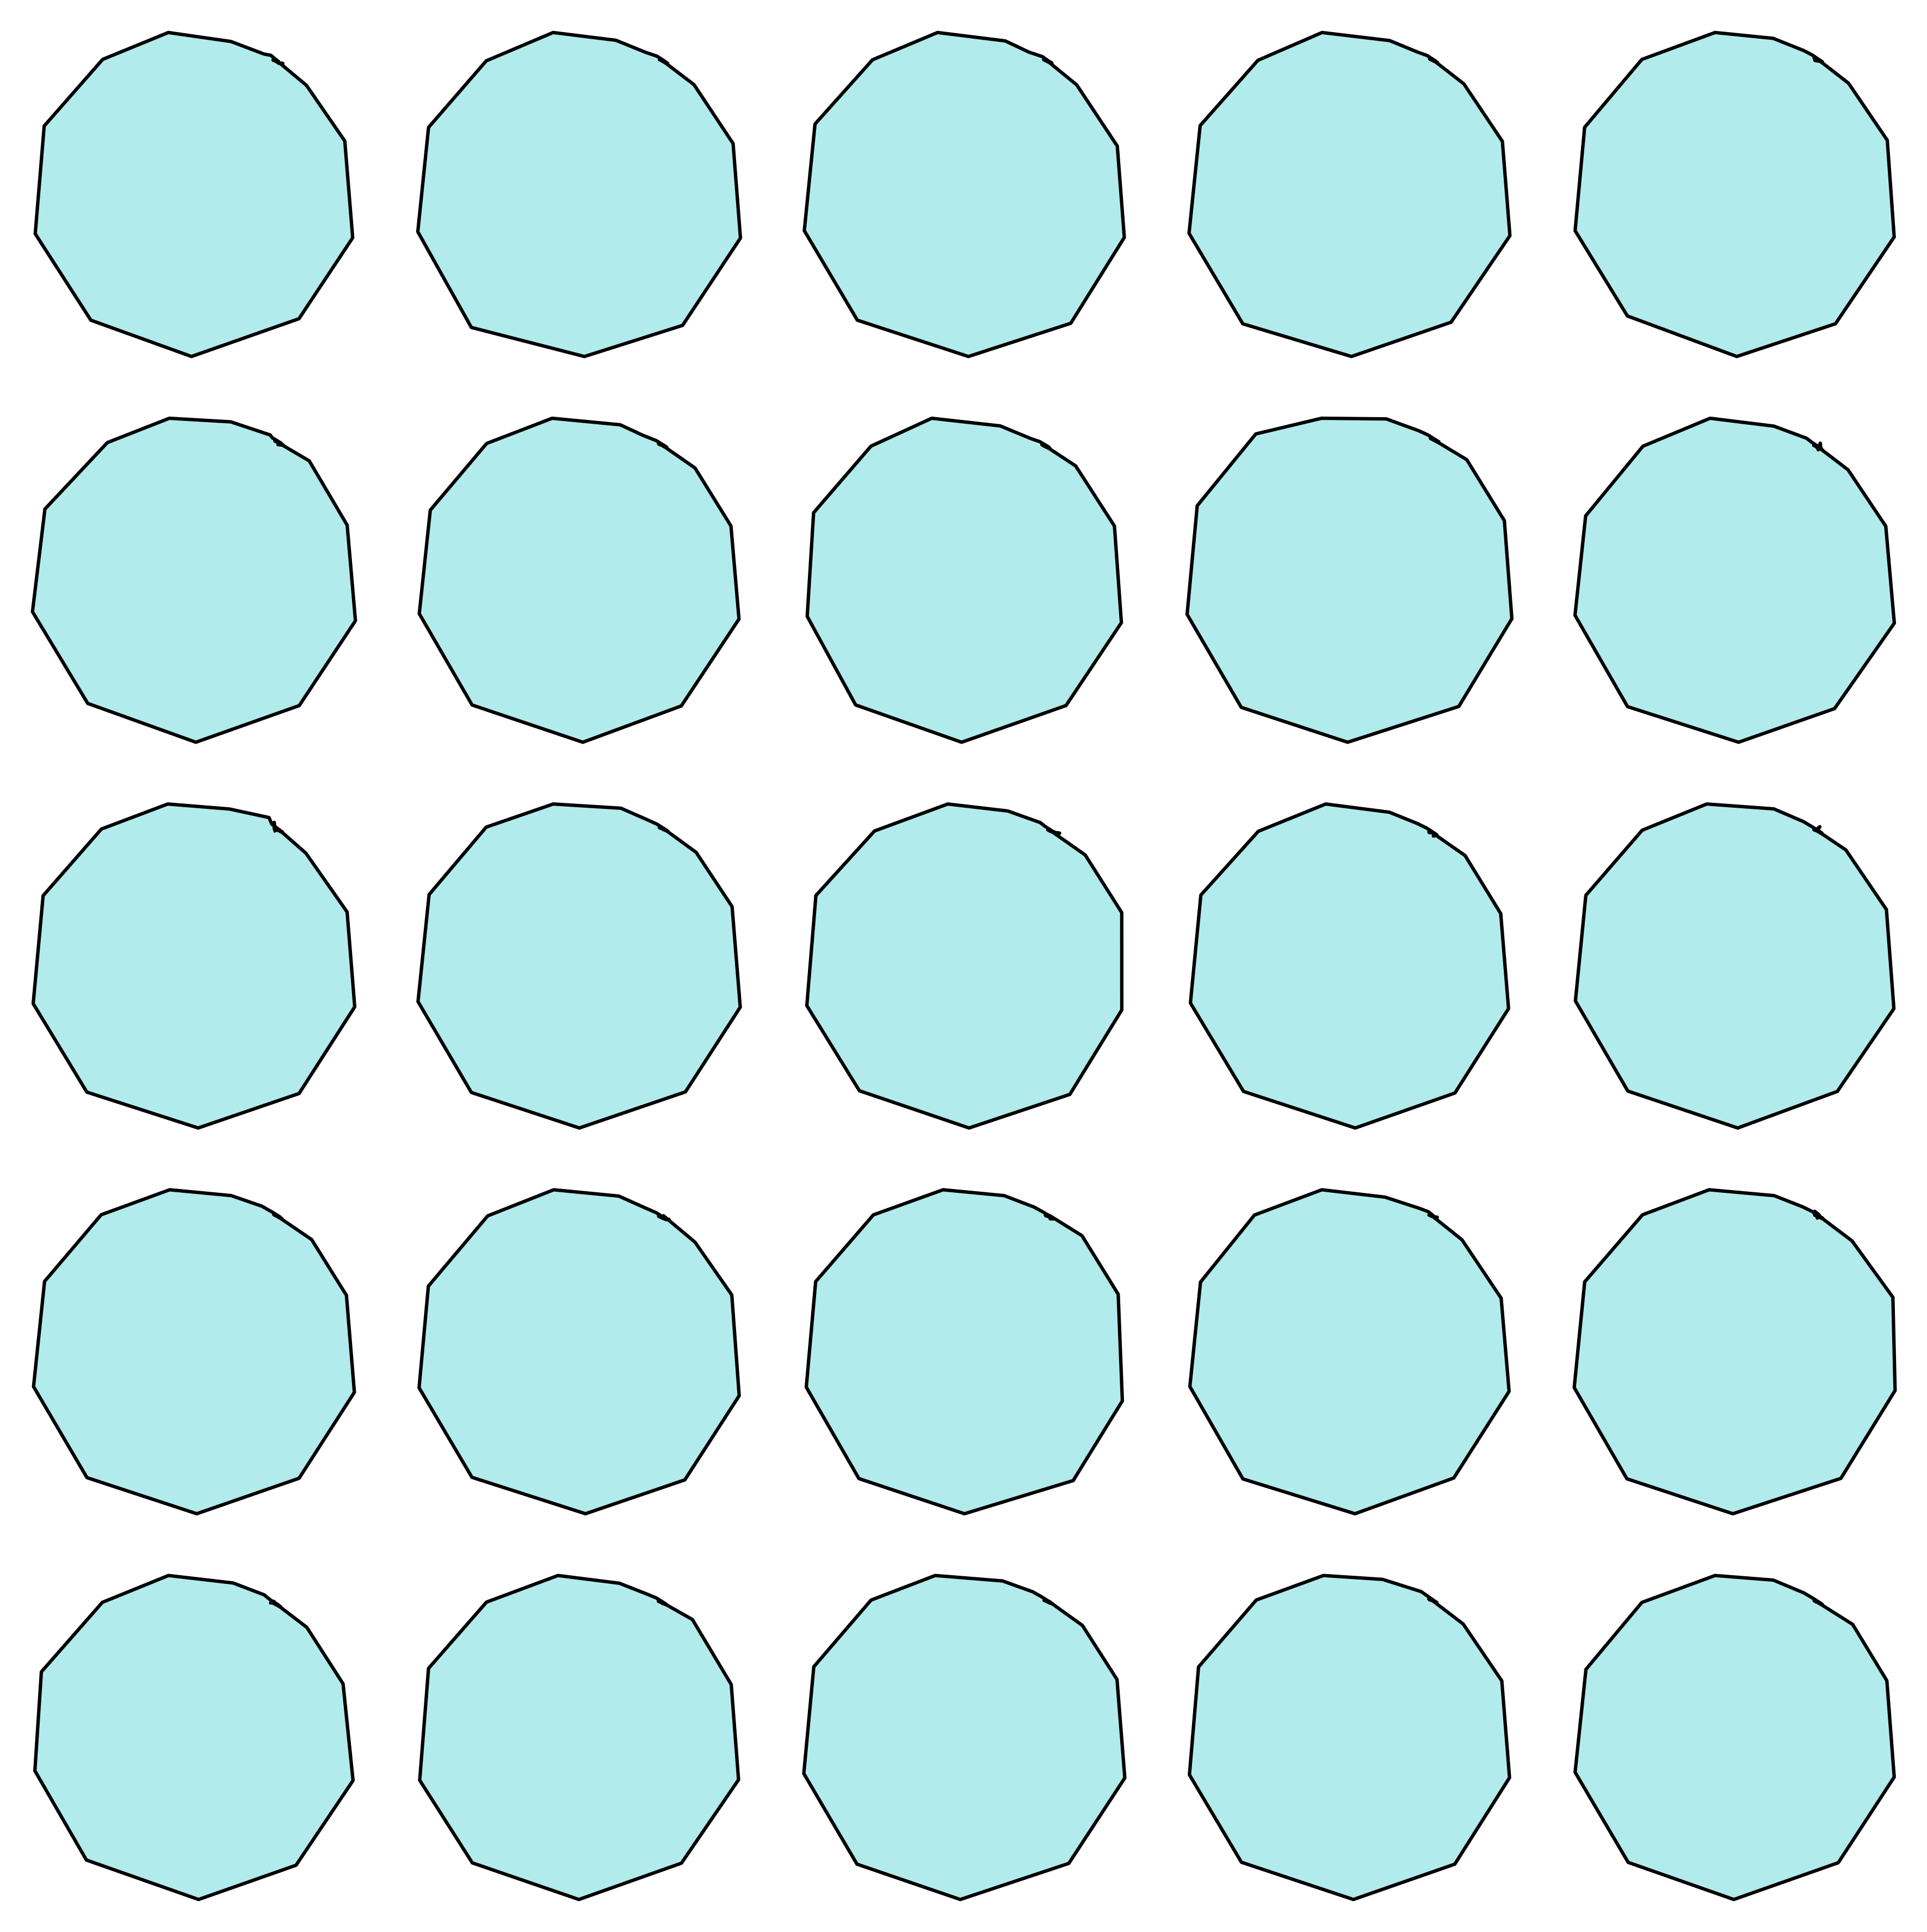
\includegraphics[width=\textwidth]{figures/GAResults/GA3/final_population.png}
        \caption{After 1000 generations of GA evolution.}
        \label{fig:GA3_final}
    \end{subfigure}
    \caption{GA3 starting and final population after optimising for compactness metric.}
    \label{fig:GA3_before_after_GA}
\end{figure}

\begin{figure}[H]
    \centering
    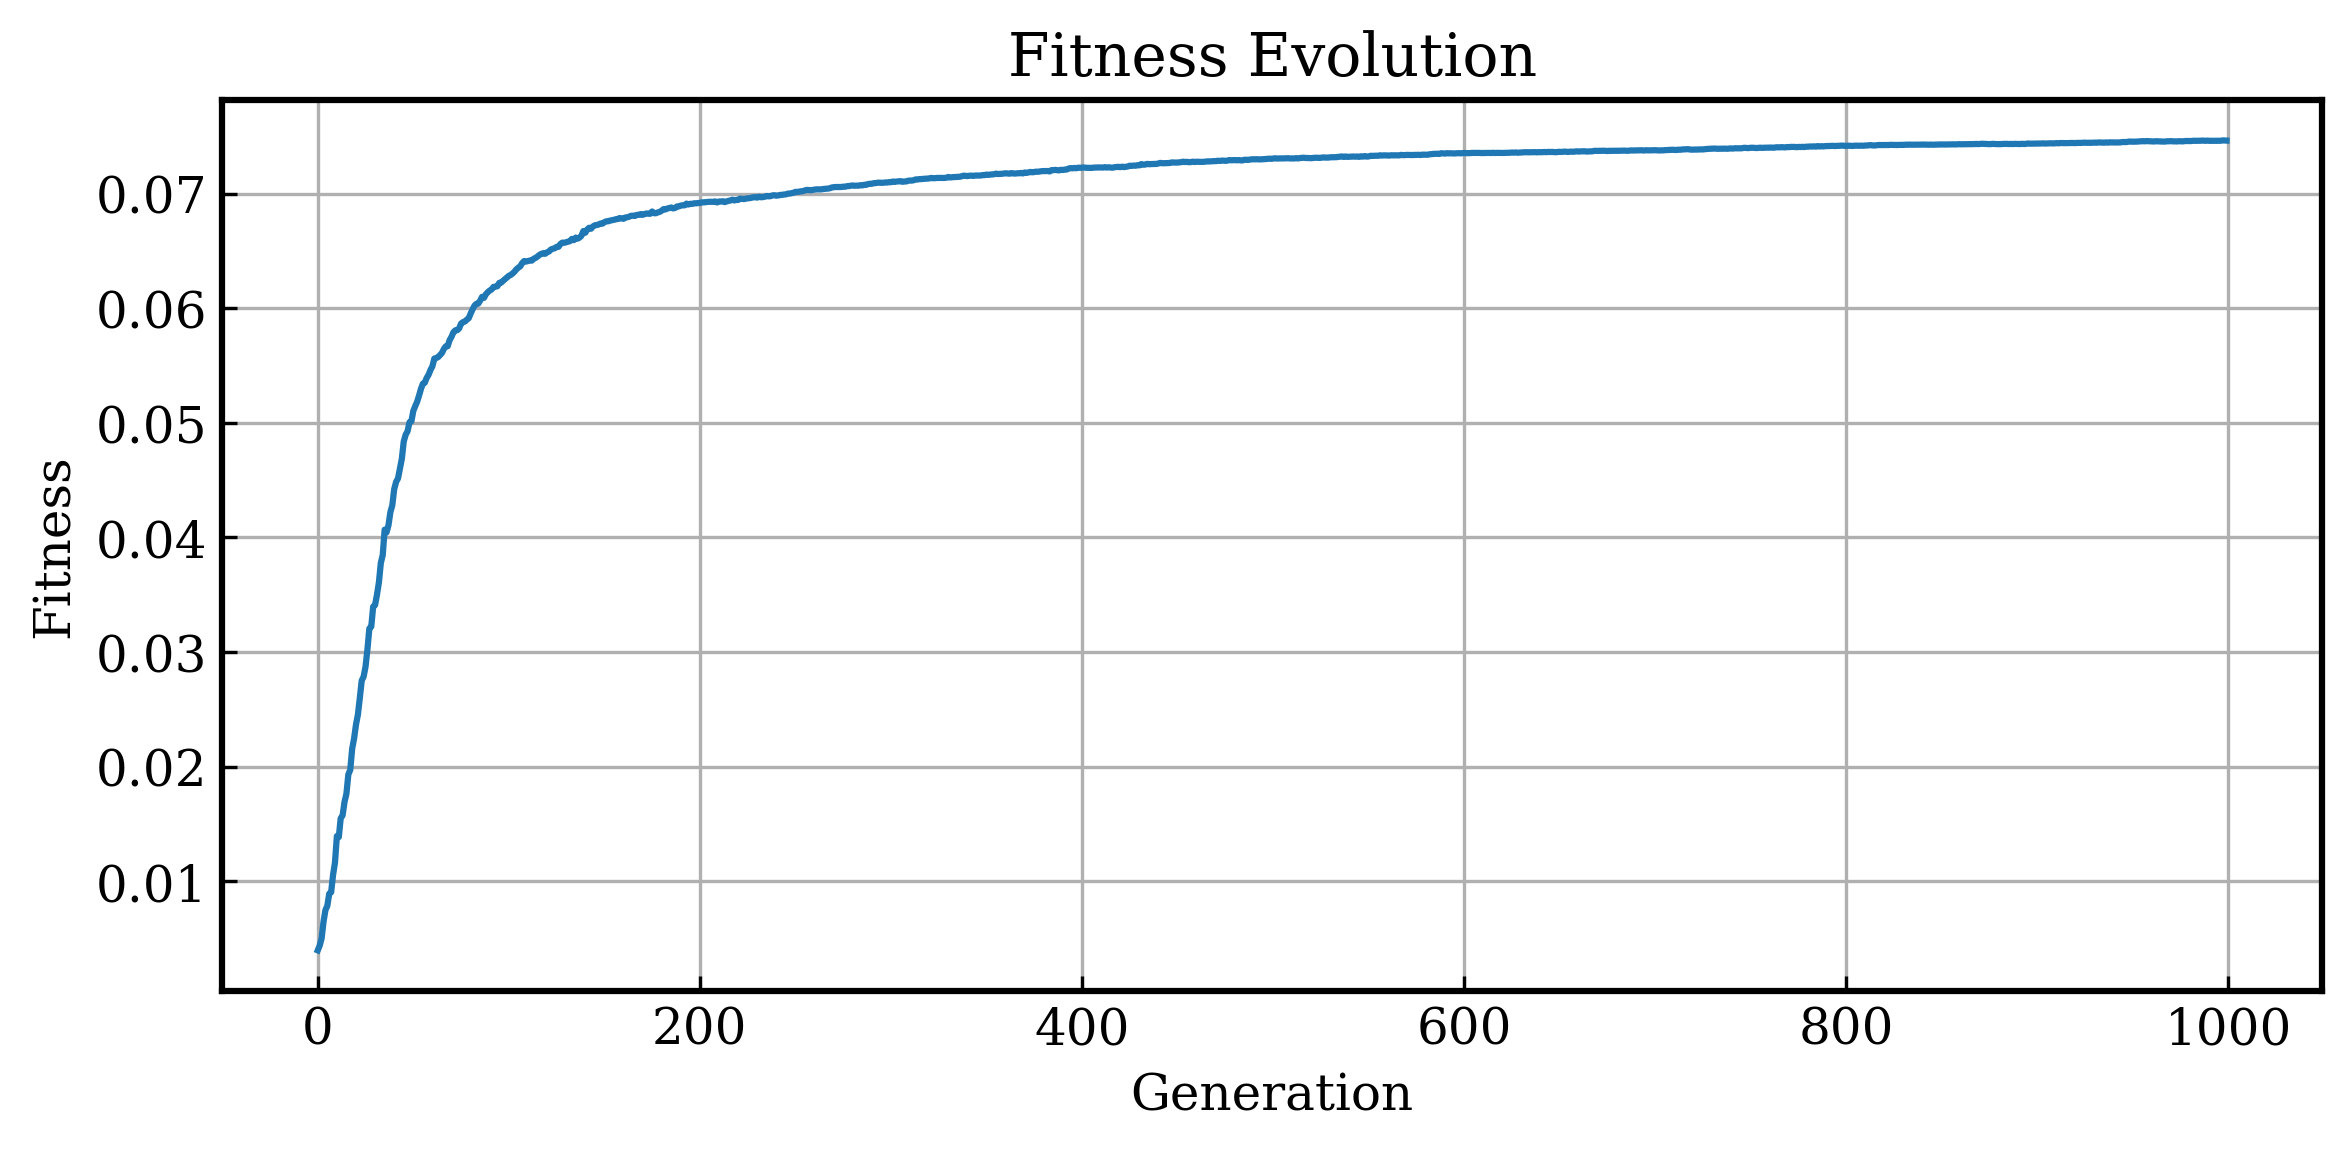
\includegraphics[width=0.75\linewidth]{figures/GAResults/GA3/1000gens_10pars_100initpop_5pcent_mut.png}
    \caption{GA3 Genetic Algorithm Fitness Score Evolution}
    \label{fig:GA3_fitness}
\end{figure}

\subsubsection*{GA4 - Random Noise Polygon: Resolution = 50; Number of Parents = 10; Initial Population = 100}
When increasing the resolution to 50 nodes, maintaining an initial population of 100 and 10 parents in the GA evolution, we see the final generation being less reflected of a circular design. This is evident in Figure~\ref{fig:GA4_before_after_GA} and the final fitness reaching only 0.07 after 1000 evolutions in the fitness curve, shown in Figure~\ref{fig:GA4_fitness}. The resultant shapes also demonstrate block like artefacts, where the optimised nodes have fixated around specific points, such as those seen accumulated in the top left of Figure~\ref{fig:GA4_final}.

\begin{figure}[H]
    \centering
    \begin{subfigure}[b]{0.45\textwidth}
        \centering
        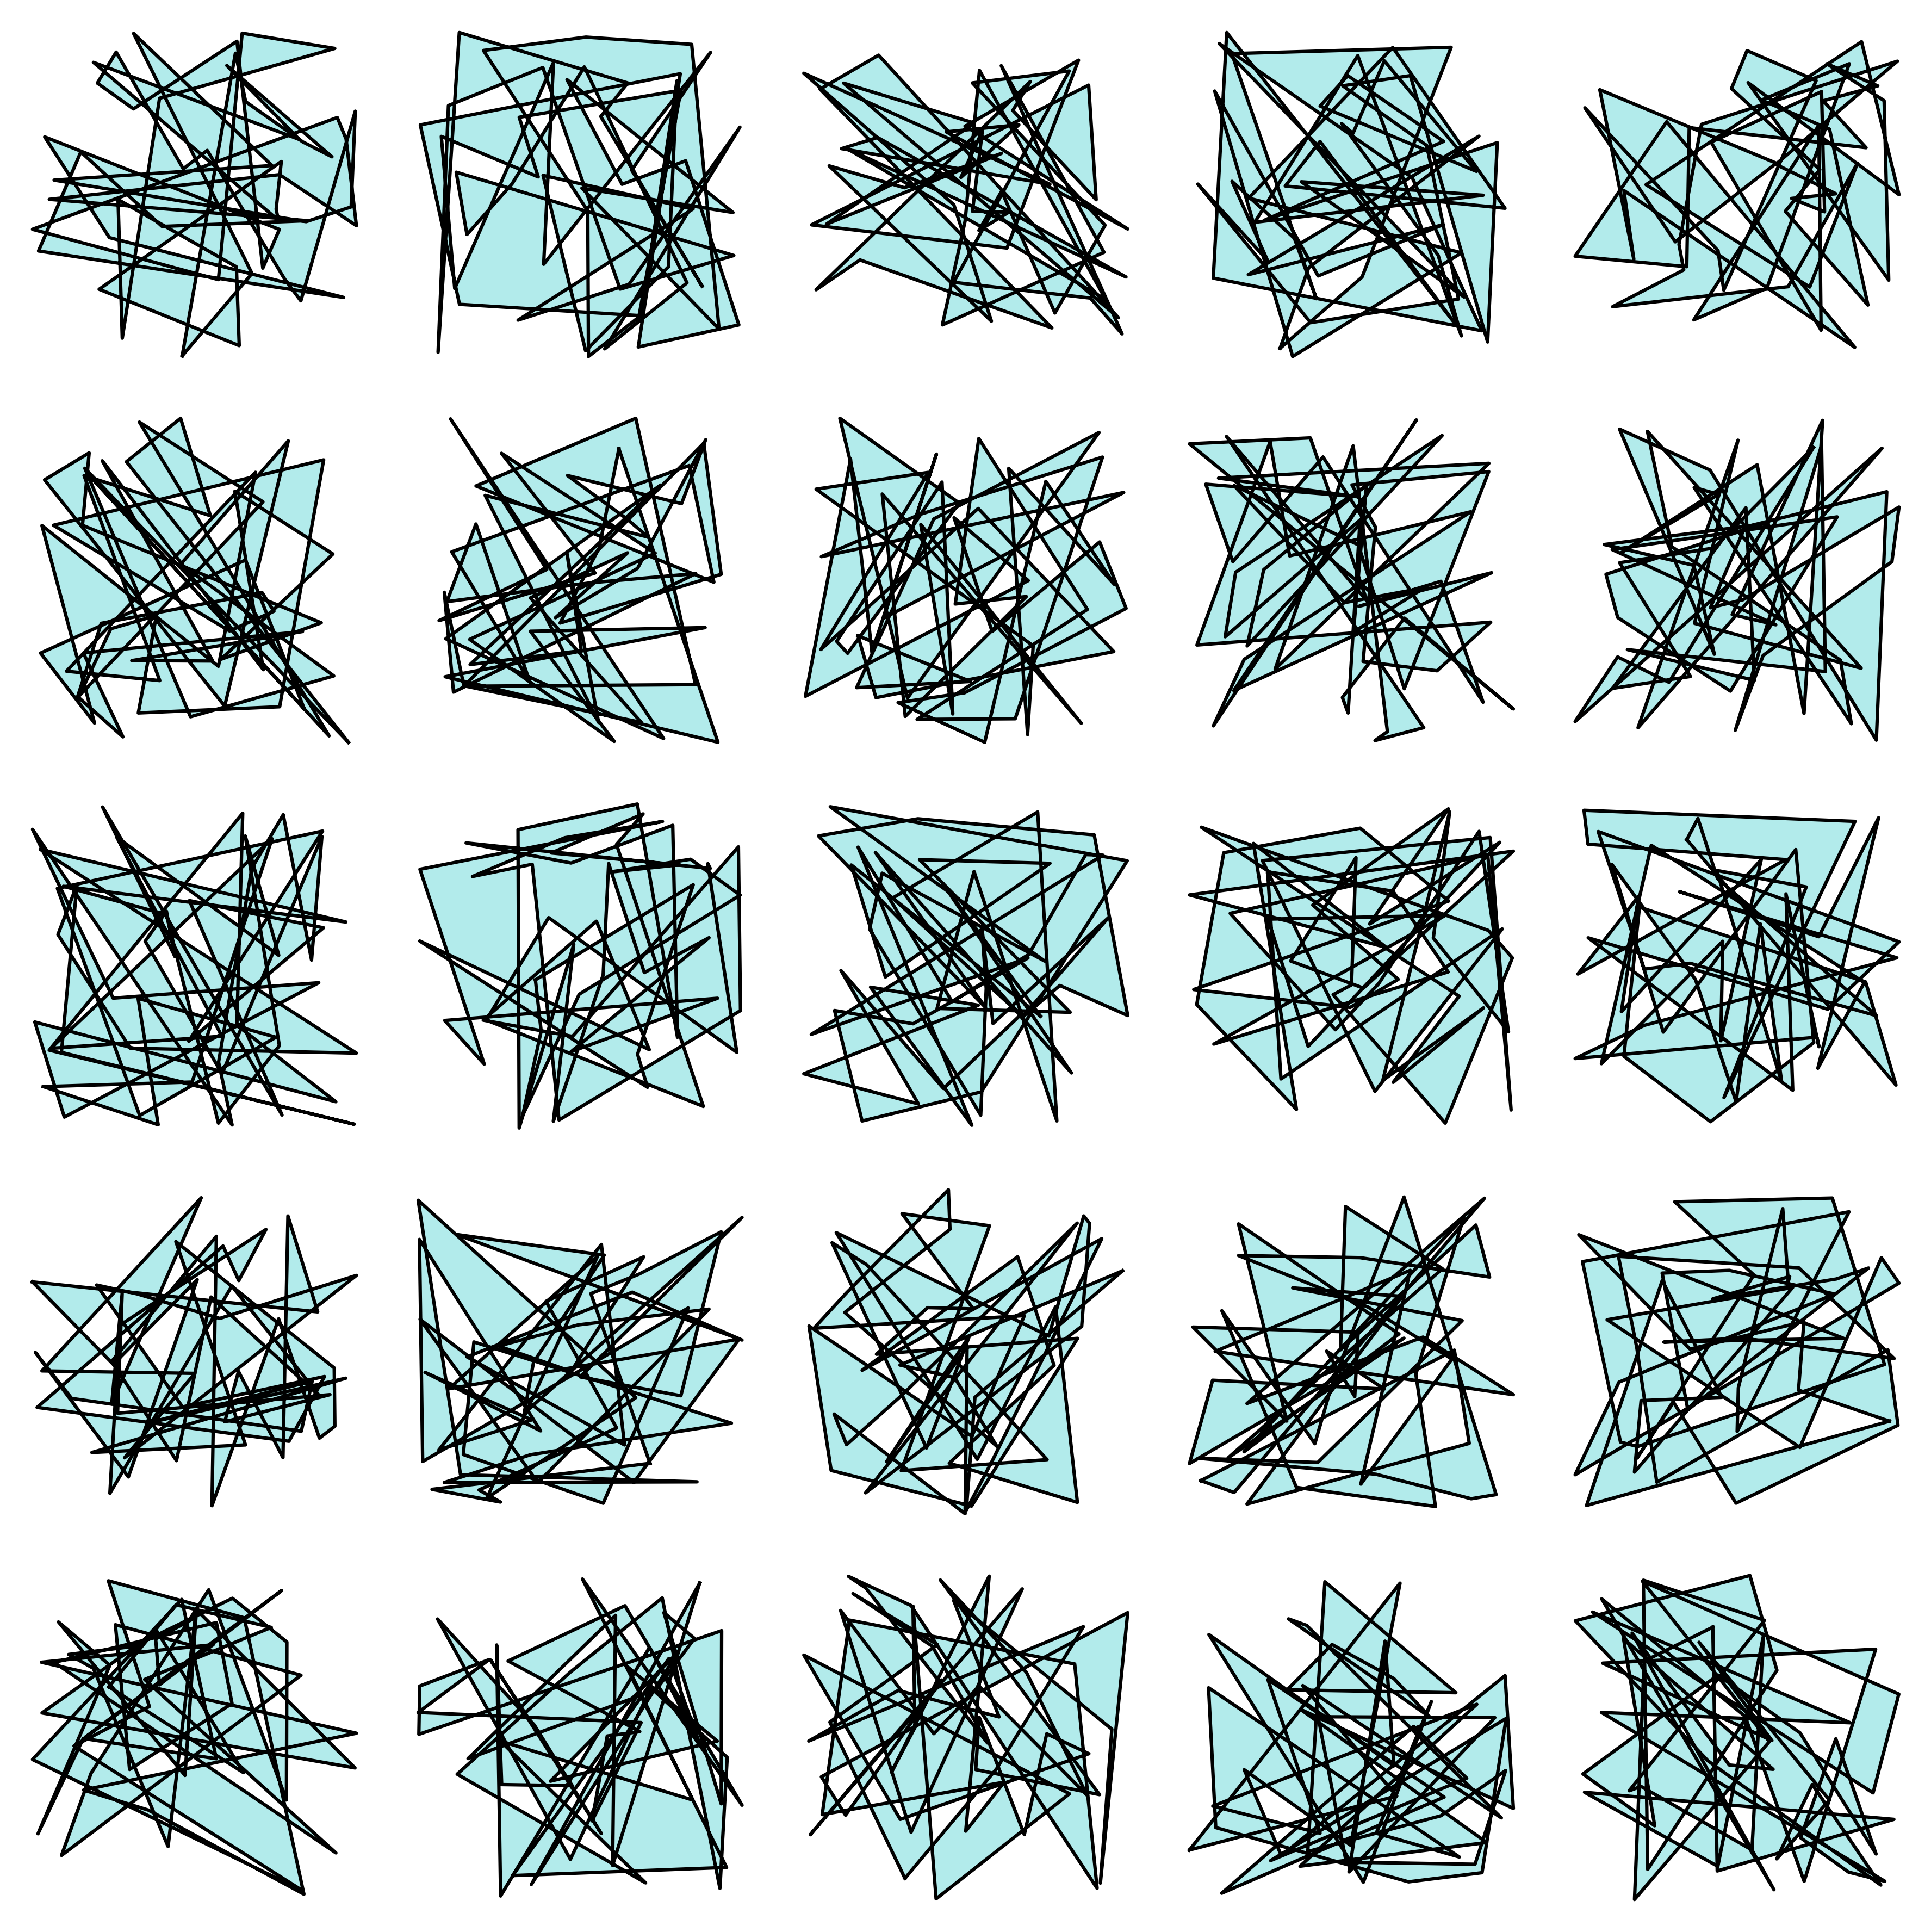
\includegraphics[width=\textwidth]{figures/GAResults/GA4/50point_initial_pop.png}
        \caption{Initial starting population}
        \label{fig:GA4_starting}
    \end{subfigure}
    \hfill
    \begin{subfigure}[b]{0.45\textwidth}
        \centering
        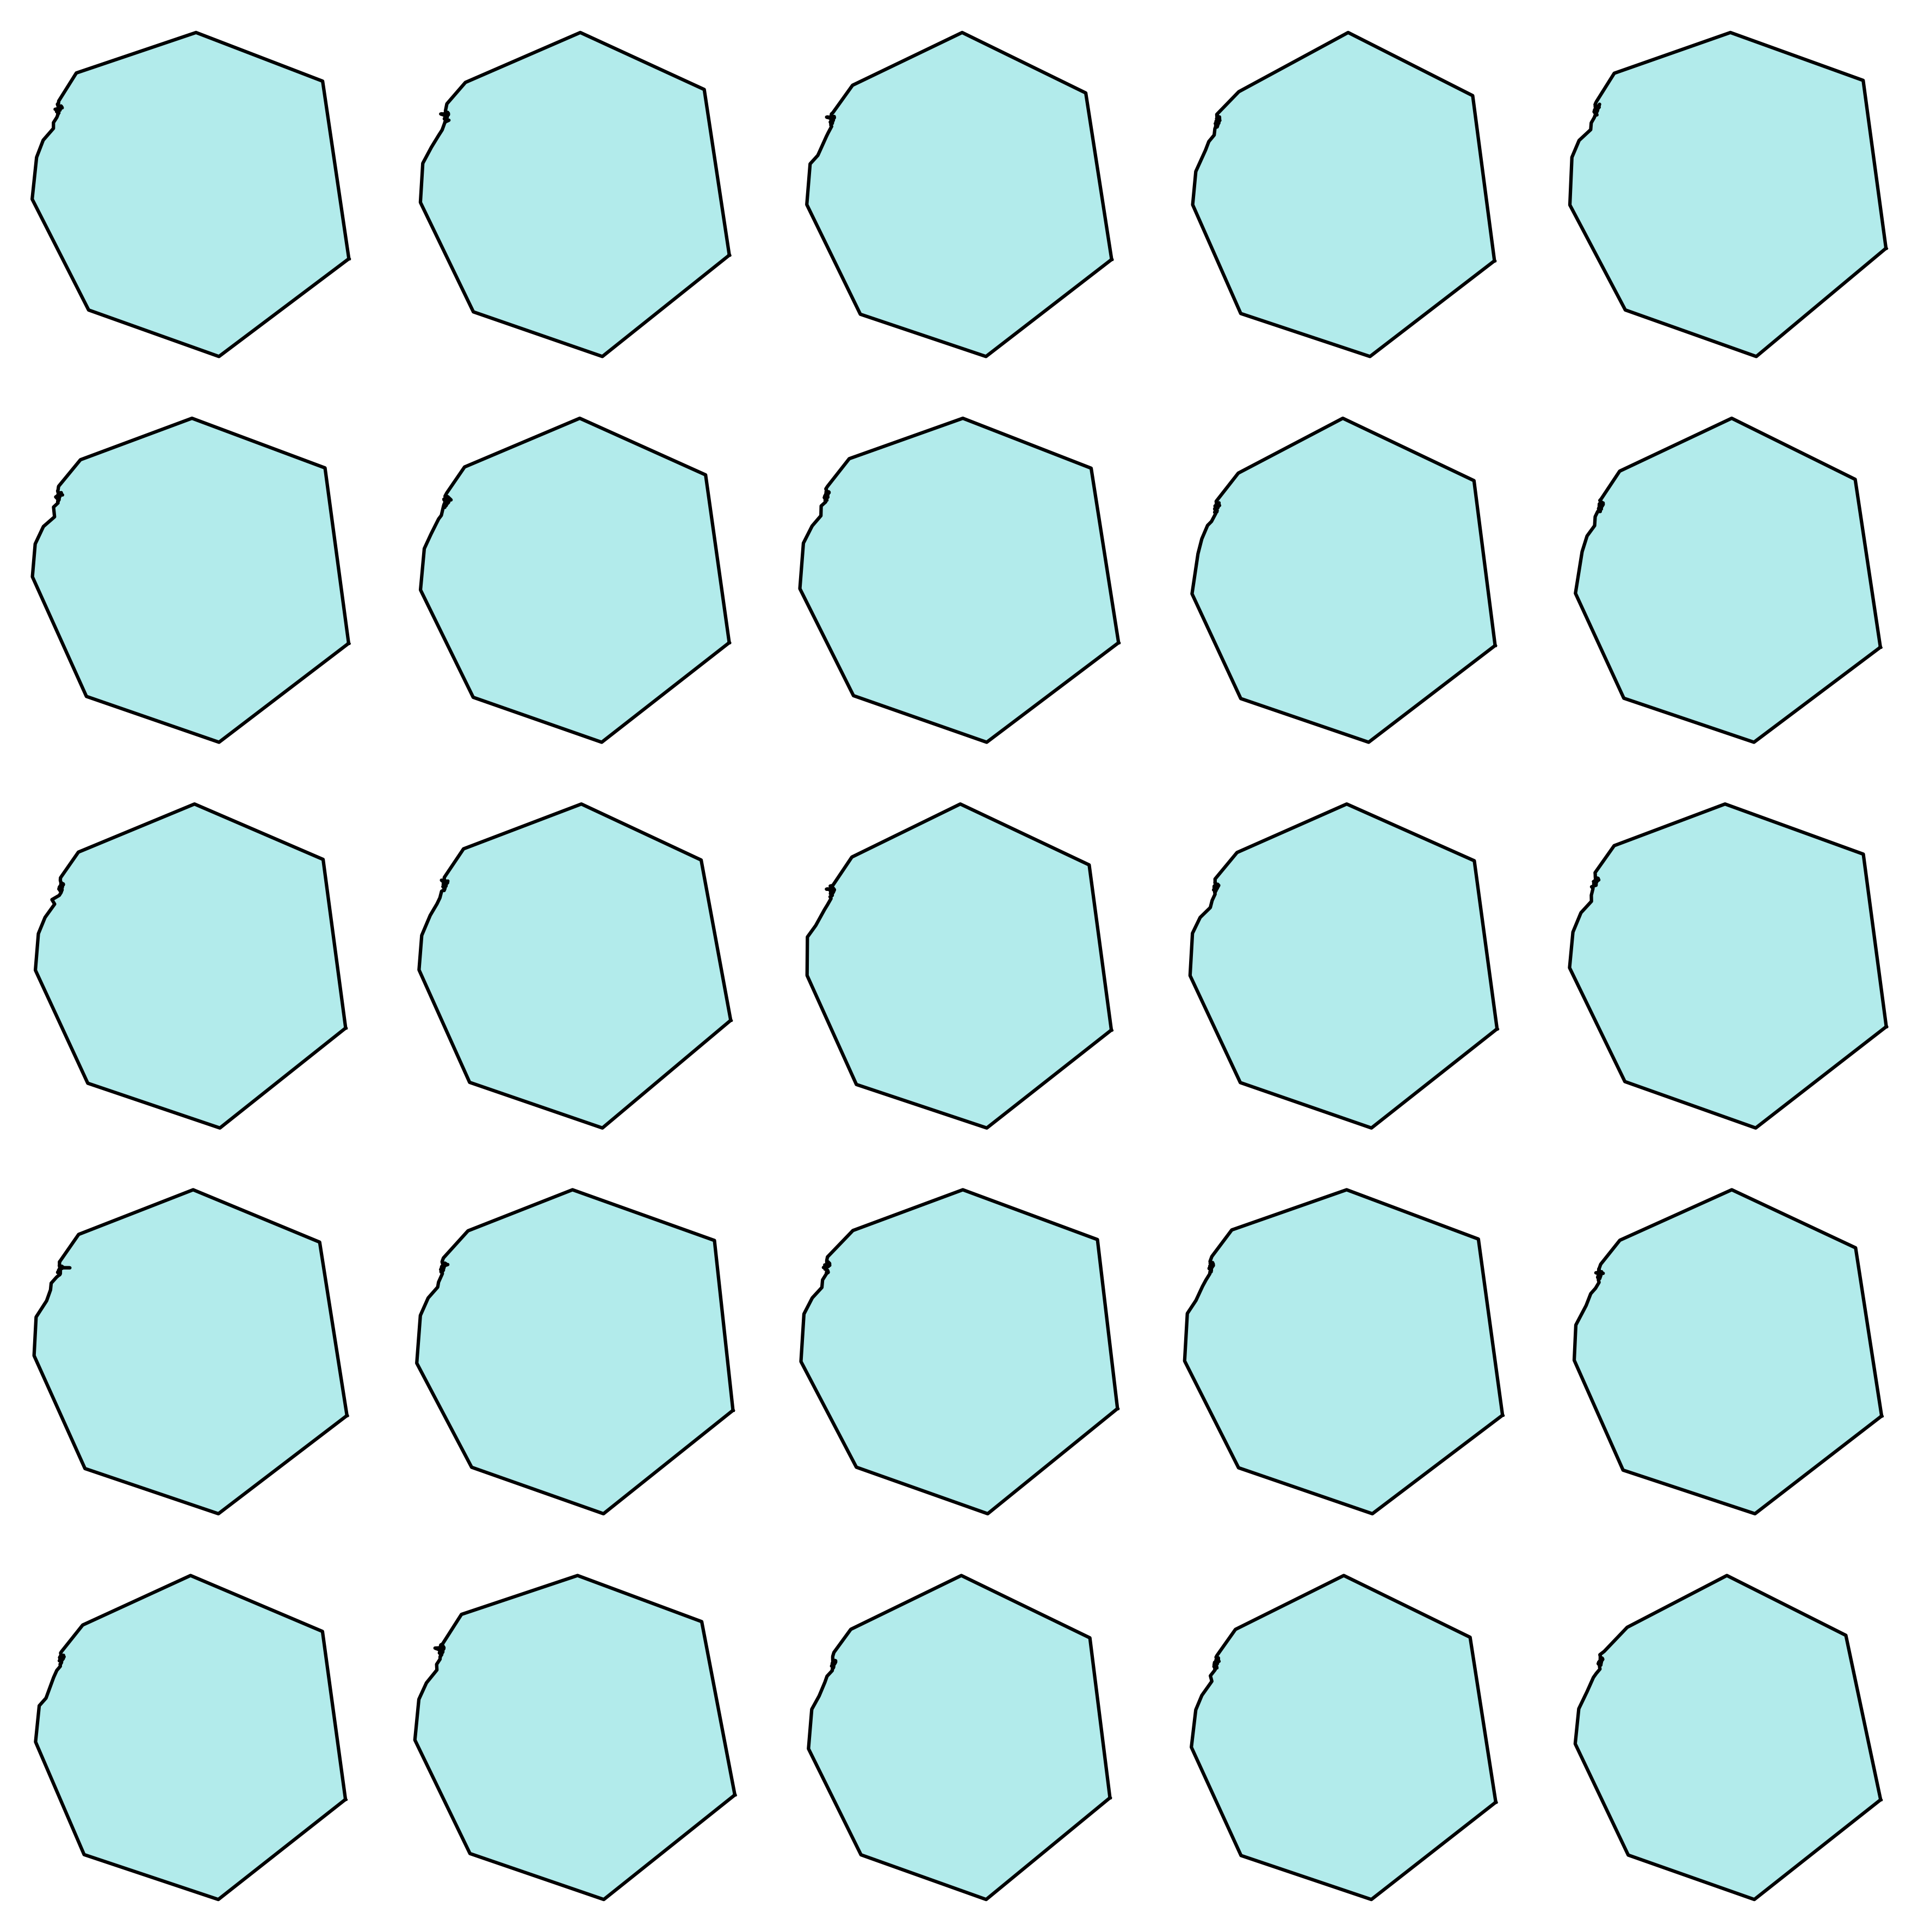
\includegraphics[width=\textwidth]{figures/GAResults/GA4/final_population.png}
        \caption{After 1000 generations of GA evolution.}
        \label{fig:GA4_final}
    \end{subfigure}
    \caption{GA4 starting and final population after optimising for compactness metric.}
    \label{fig:GA4_before_after_GA}
\end{figure}

\begin{figure}[H]
    \centering
    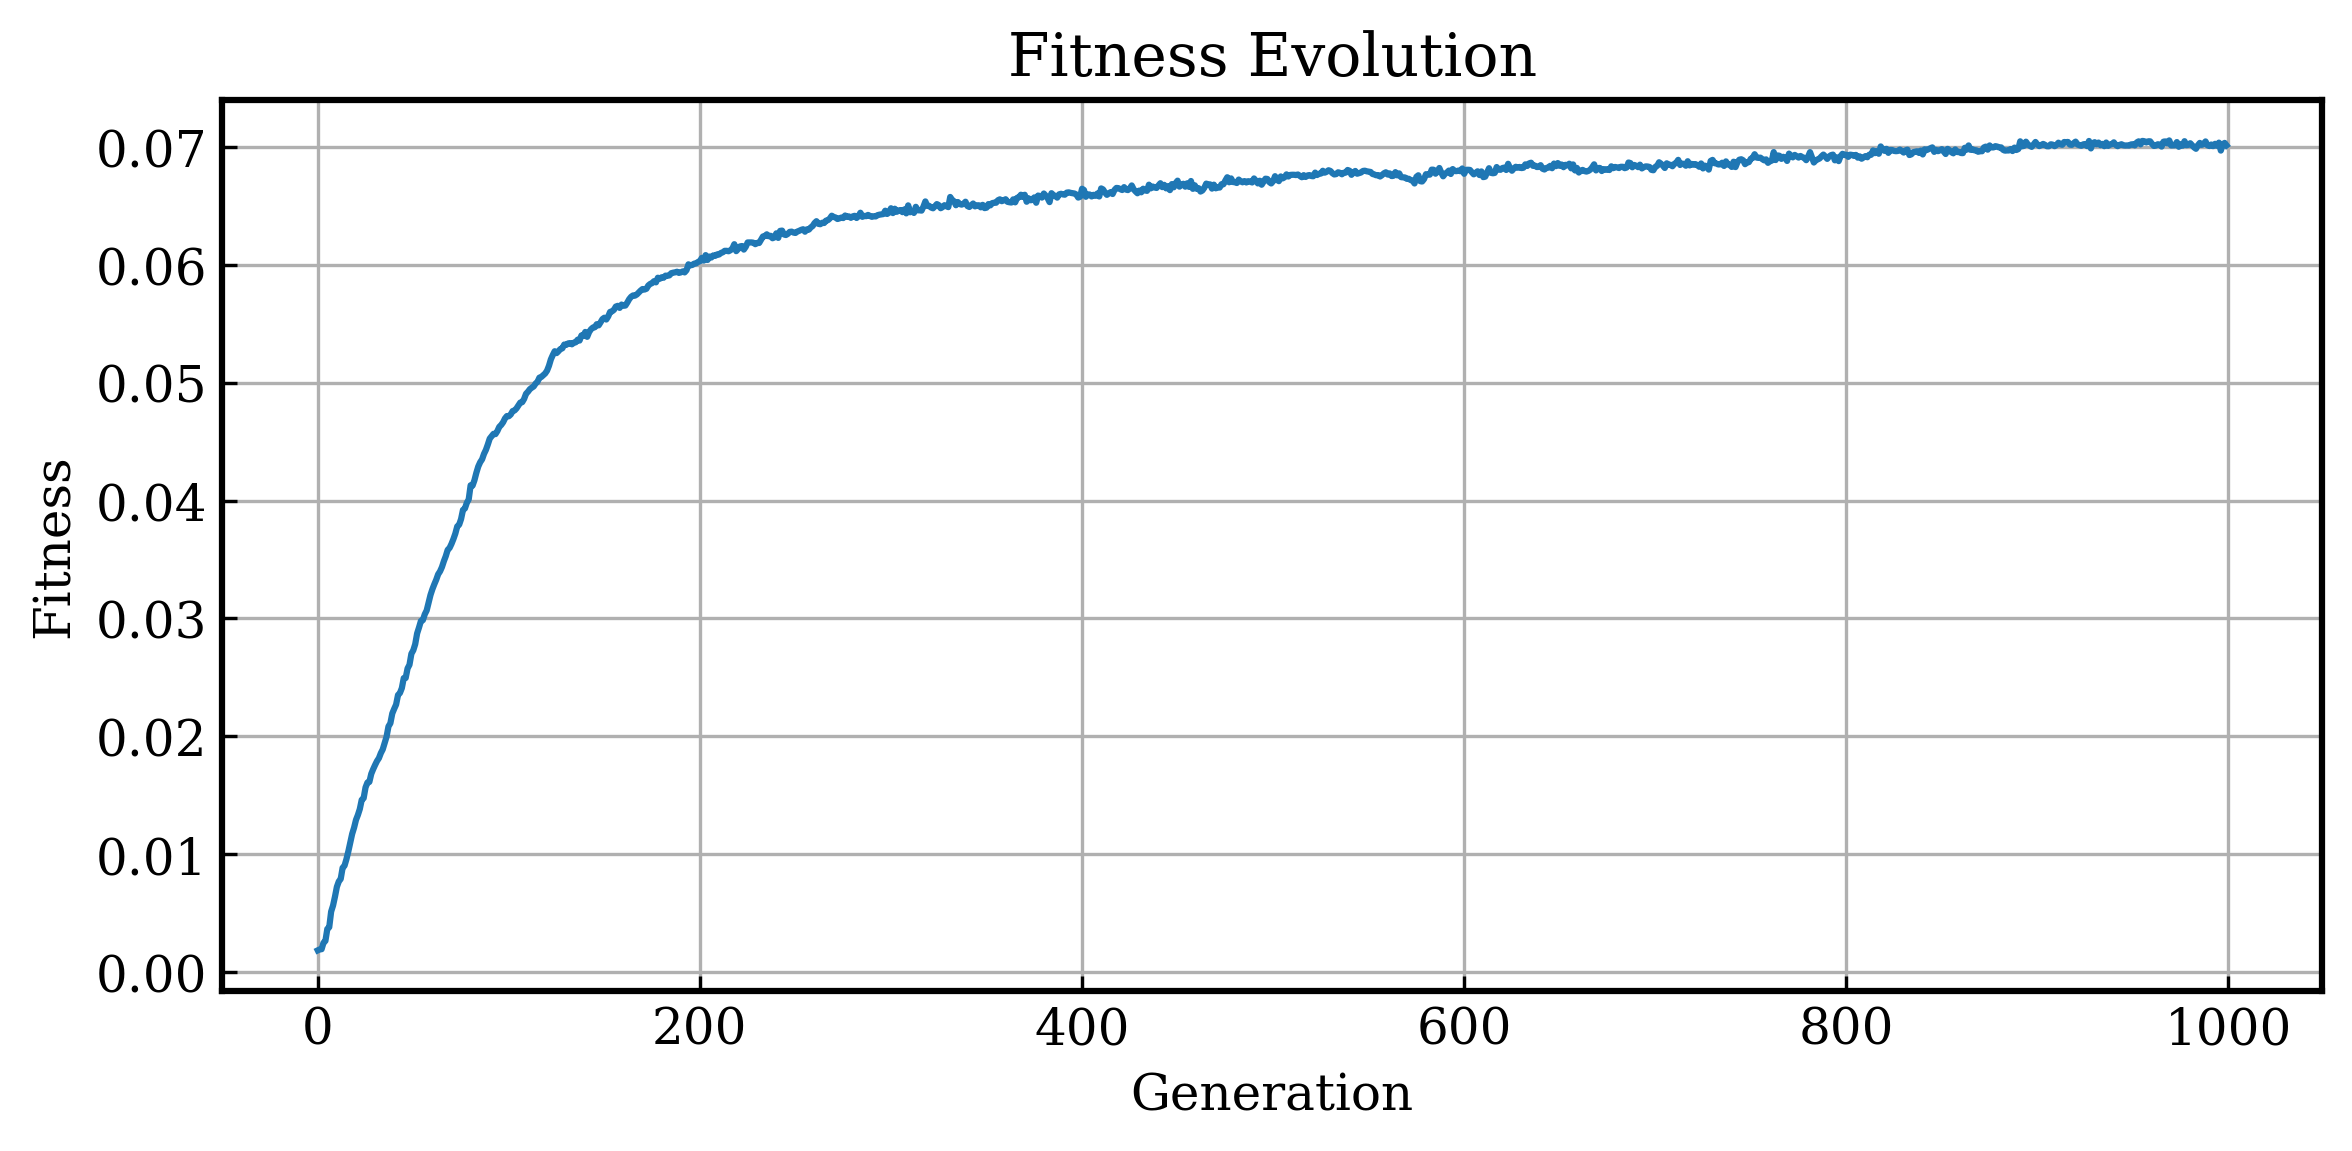
\includegraphics[width=0.75\linewidth]{figures/GAResults/GA4/1000gens_10pars_100initpop_5pcent_mut.png}
    \caption{GA4 Genetic Algorithm Fitness Score Evolution}
    \label{fig:GA4_fitness}
\end{figure}

\subsubsection*{GA5 - Random Noise Polygon: Resolution = 100; Number of Parents = 10; Initial Population = 100}
Doubling the resolution of the design problem to 100 reveals a significant drop off in the ability of the genetic algorithm to optimise for compactness, despite evolving for 1000 generations. For such high resolutions, it is expected that increasing the initial population, or evolving for more generations may suffice to find an optimal solution, however, in the context of engineering design this is not always a tractable luxury to assume. Often data is sparse, or computationally expensive to generate, and therefore evaluating so many samples is not possible.
The fitness curve also demonstrates deterioration in performance with a final maximum fitness value in the population of 0.06 - a 20 \% reduction in fitness. In engineering, this may correspond to a 20\% reduction in component performance, which could easily translate into a equal or greater loss (due to multi-physics effects) in efficiency. For example, a loss of 20\% aero-efficiency in turbo-machinery components could be detrimental to engine performance.

\begin{figure}[H]
    \centering
    \begin{subfigure}[b]{0.45\textwidth}
        \centering
        \includegraphics[width=\textwidth]{figures/GAResults/GA5/100point_initial_pop.png}
        \caption{Initial starting population}
        \label{fig:GA5_starting}
    \end{subfigure}
    \hfill
    \begin{subfigure}[b]{0.45\textwidth}
        \centering
        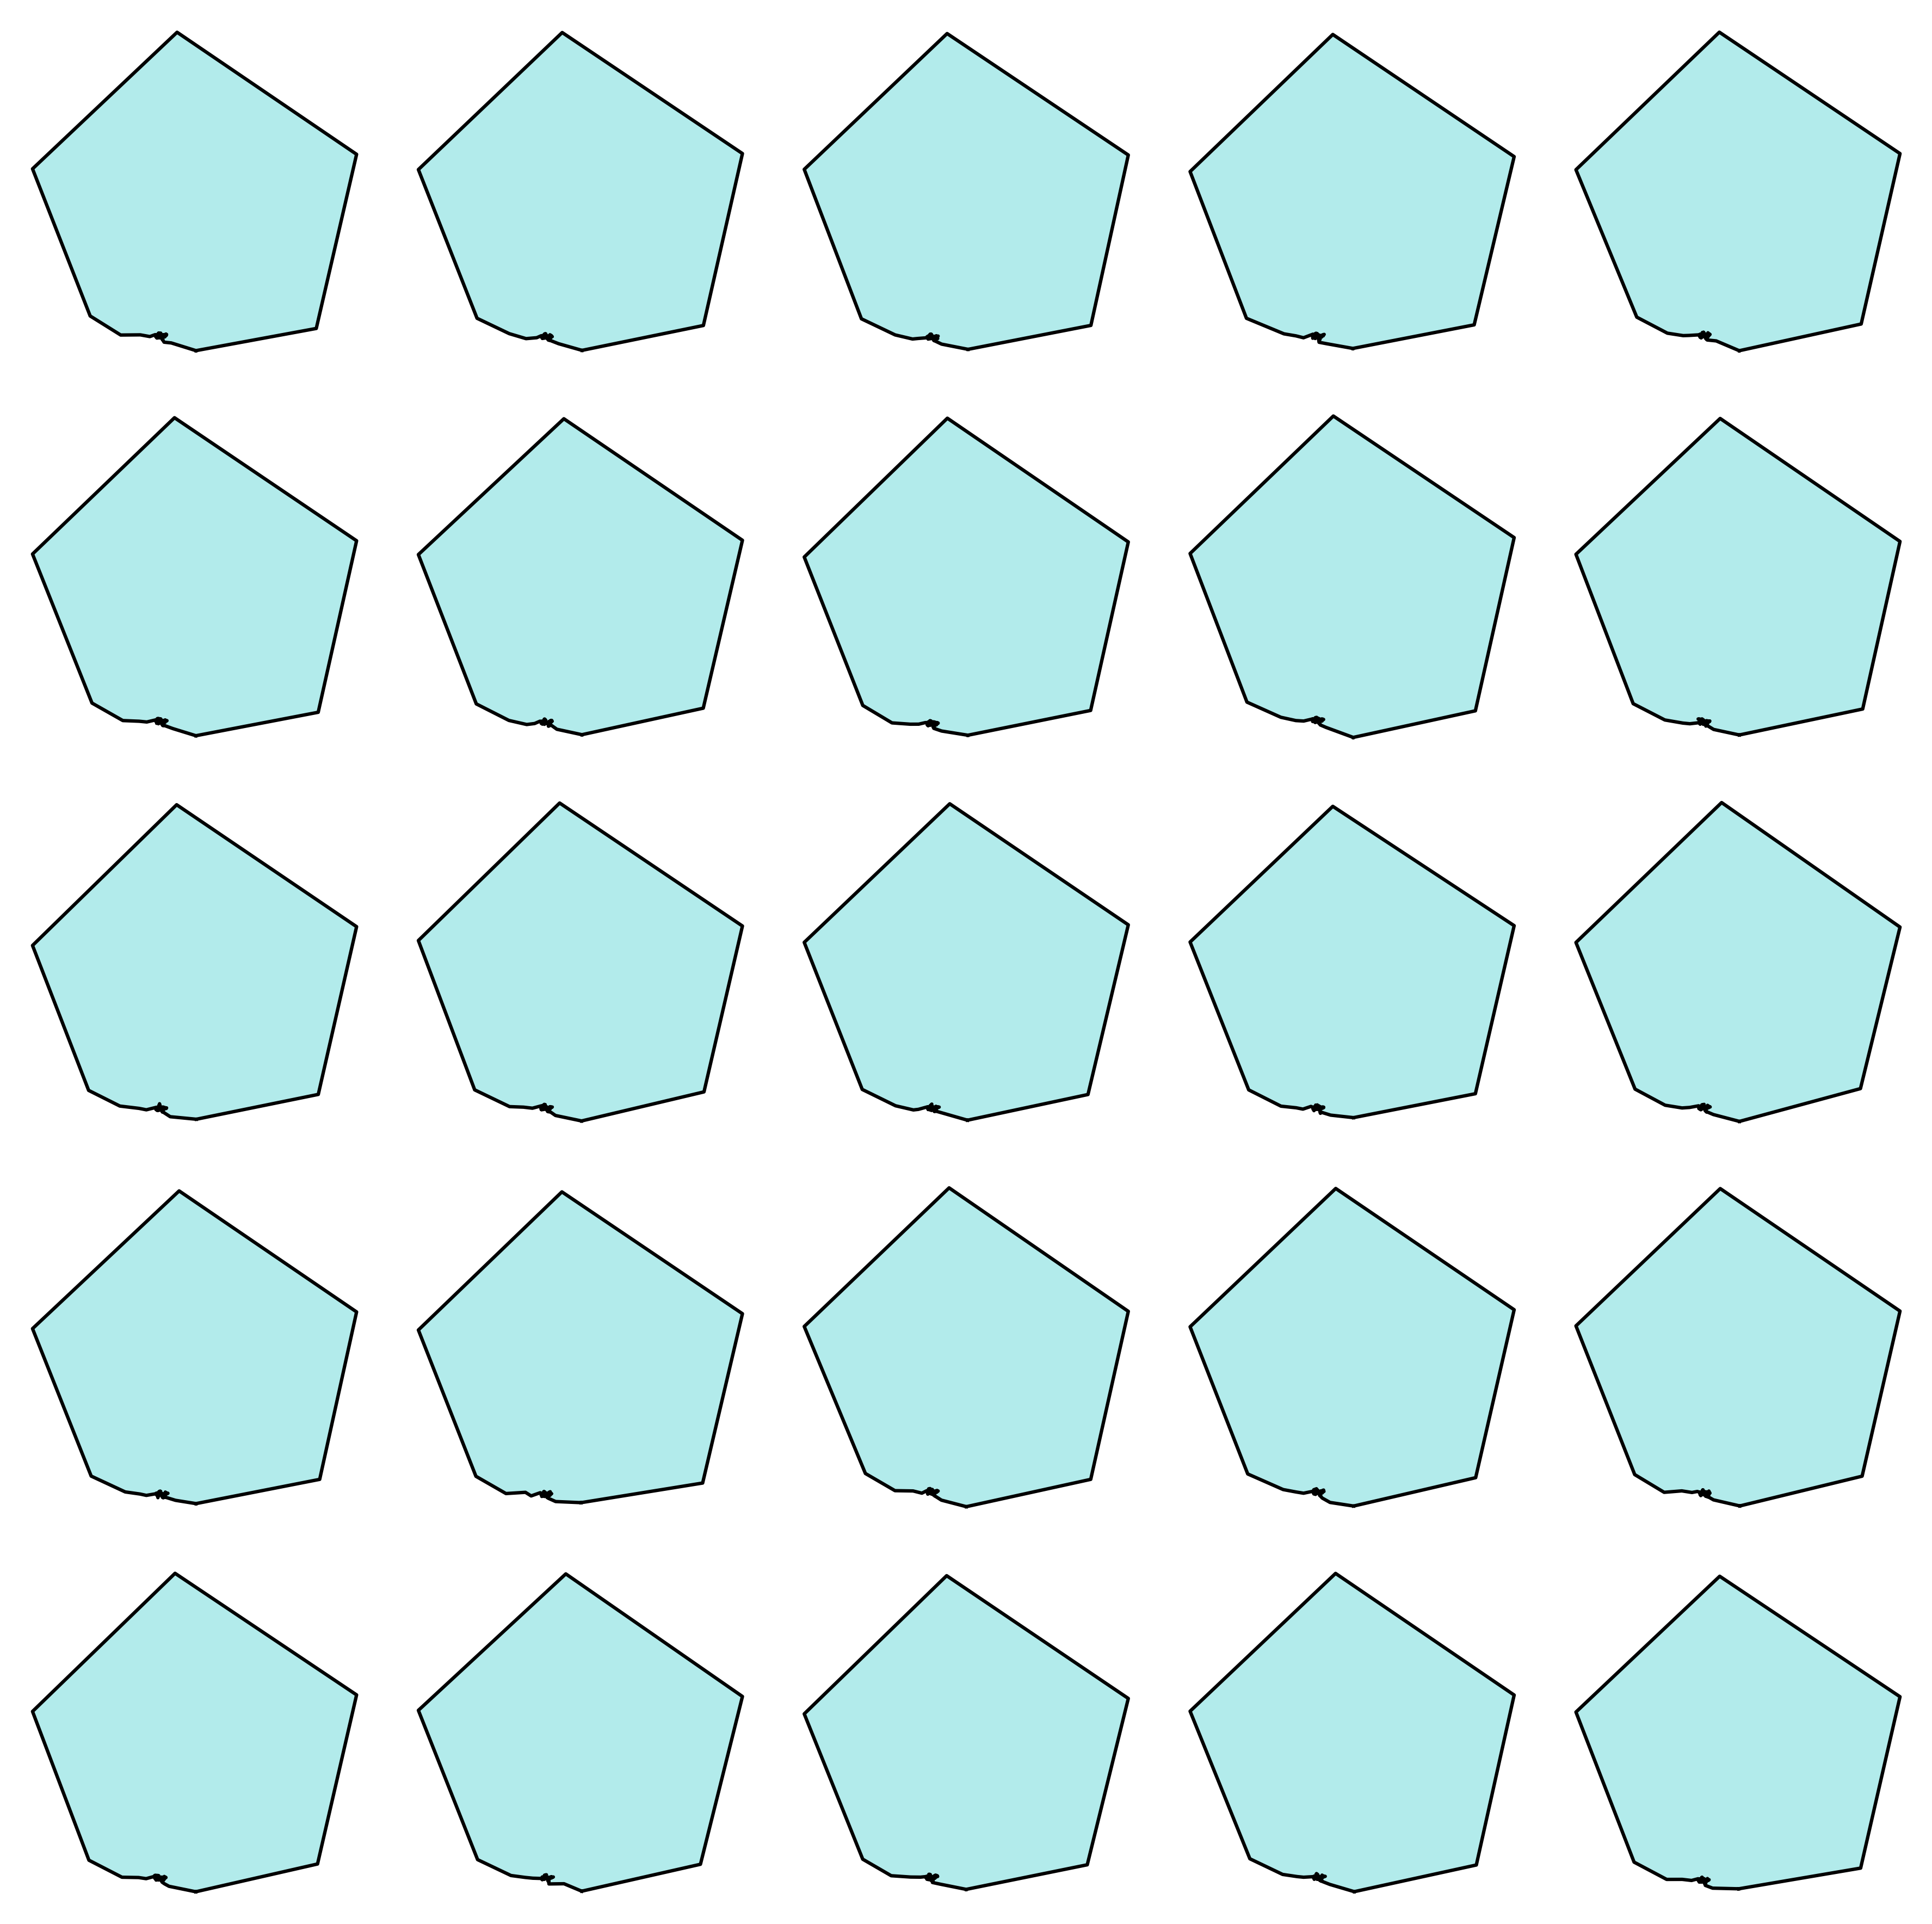
\includegraphics[width=\textwidth]{figures/GAResults/GA5/final_population.png}
        \caption{After 1000 generations of GA evolution.}
        \label{fig:GA5_final}
    \end{subfigure}
    \caption{GA5 starting and final population after optimising for compactness metric.}
    \label{fig:GA5_before_after_GA}
\end{figure}

\begin{figure}[H]
    \centering
    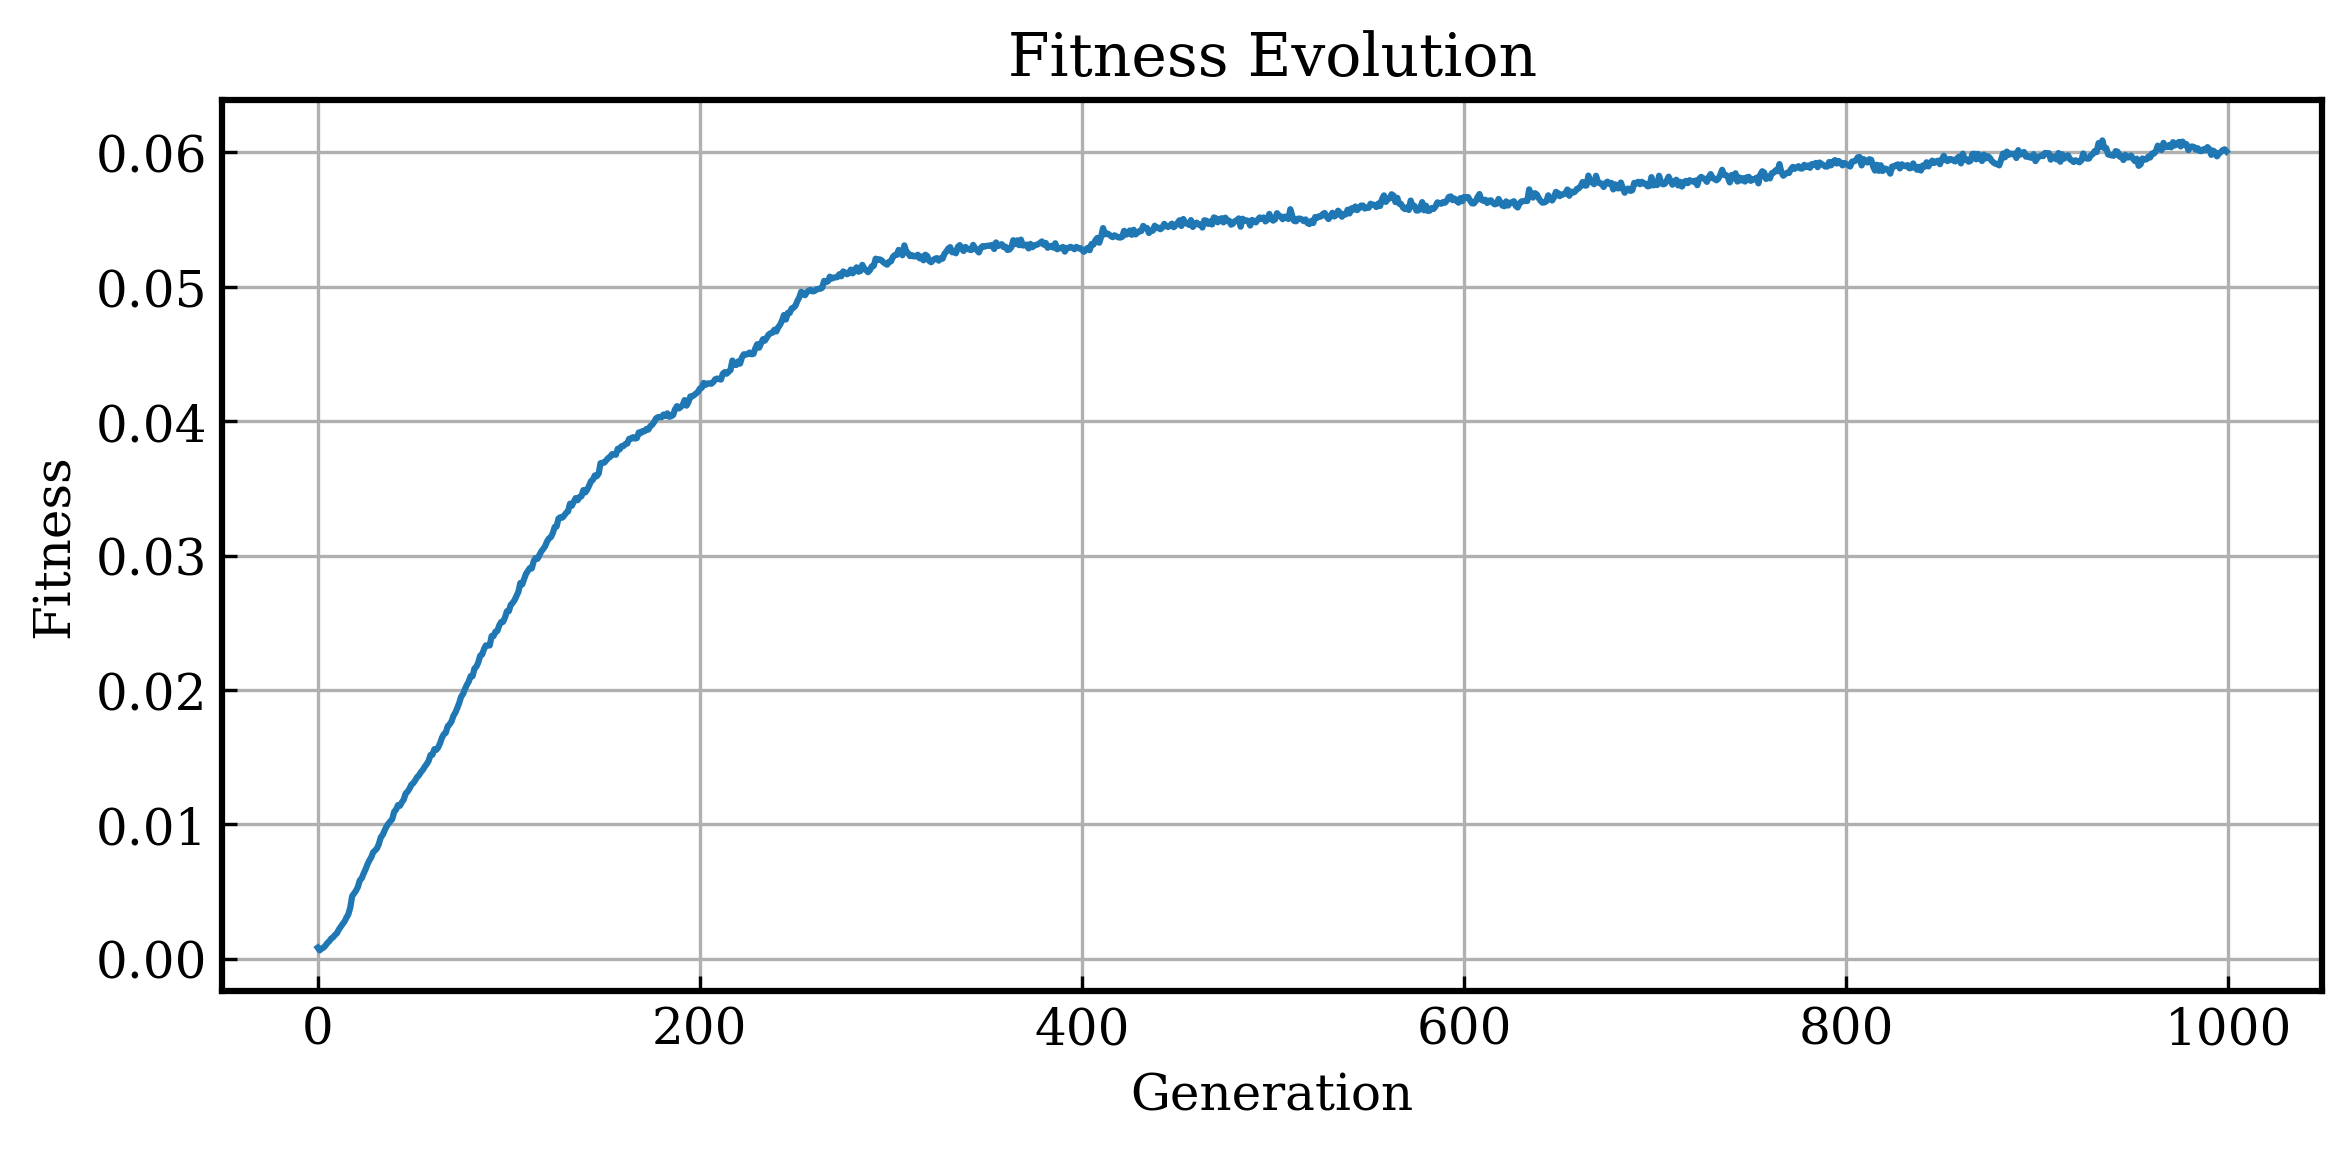
\includegraphics[width=0.75\linewidth]{figures/GAResults/GA5/1000gens_10pars_100initpop_5pcent_mut.png}
    \caption{GA5 Genetic Algorithm Fitness Score Evolution}
    \label{fig:GA5_fitness}
\end{figure}

\subsubsection*{GA6 - Random Noise Polygon: Resolution = 200; Number of Parents = 4; Initial Population = 100}

In Figure~\ref{fig:GA6_before_after_GA}, we see the final generation is only a variation of the original noise with the GA aggregating on a final solution that places a noticeable fraction of the geometry nodes in one region. The fitness curve in this example has not plateaued at all, with a continuously increasing curve that only surpasses 0.03 after 1000 generations. This reflects a greater than 50\% reduction in fitness compared to the original low-dimensional optimisation achieved in GA1, seen in Figure~\ref{fig:GA1_before_after_GA}. We purposely demonstrate the performance here with a low number of parents used in the population competition during crossover, reflecting exploitation versus exploration. If we increase the number of parents to 20 while maintaining the same initial population size and number of generations, Figure~\ref{fig:GA8_before_after_GA} and Figure~\ref{fig:GA8_fitness} demonstrates improvement in the GA's ability to iterate towards a higher fitness value, with a final fitness of 0.07 after 1000 generations.

\begin{figure}[H]
    \centering
    \begin{subfigure}[b]{0.45\textwidth}
        \centering
        \includegraphics[width=\textwidth]{figures/GAResults/GA6/200point_initial_pop.png}
        \caption{Initial starting population}
        \label{fig:GA6_starting}
    \end{subfigure}
    \hfill
    \begin{subfigure}[b]{0.45\textwidth}
        \centering
        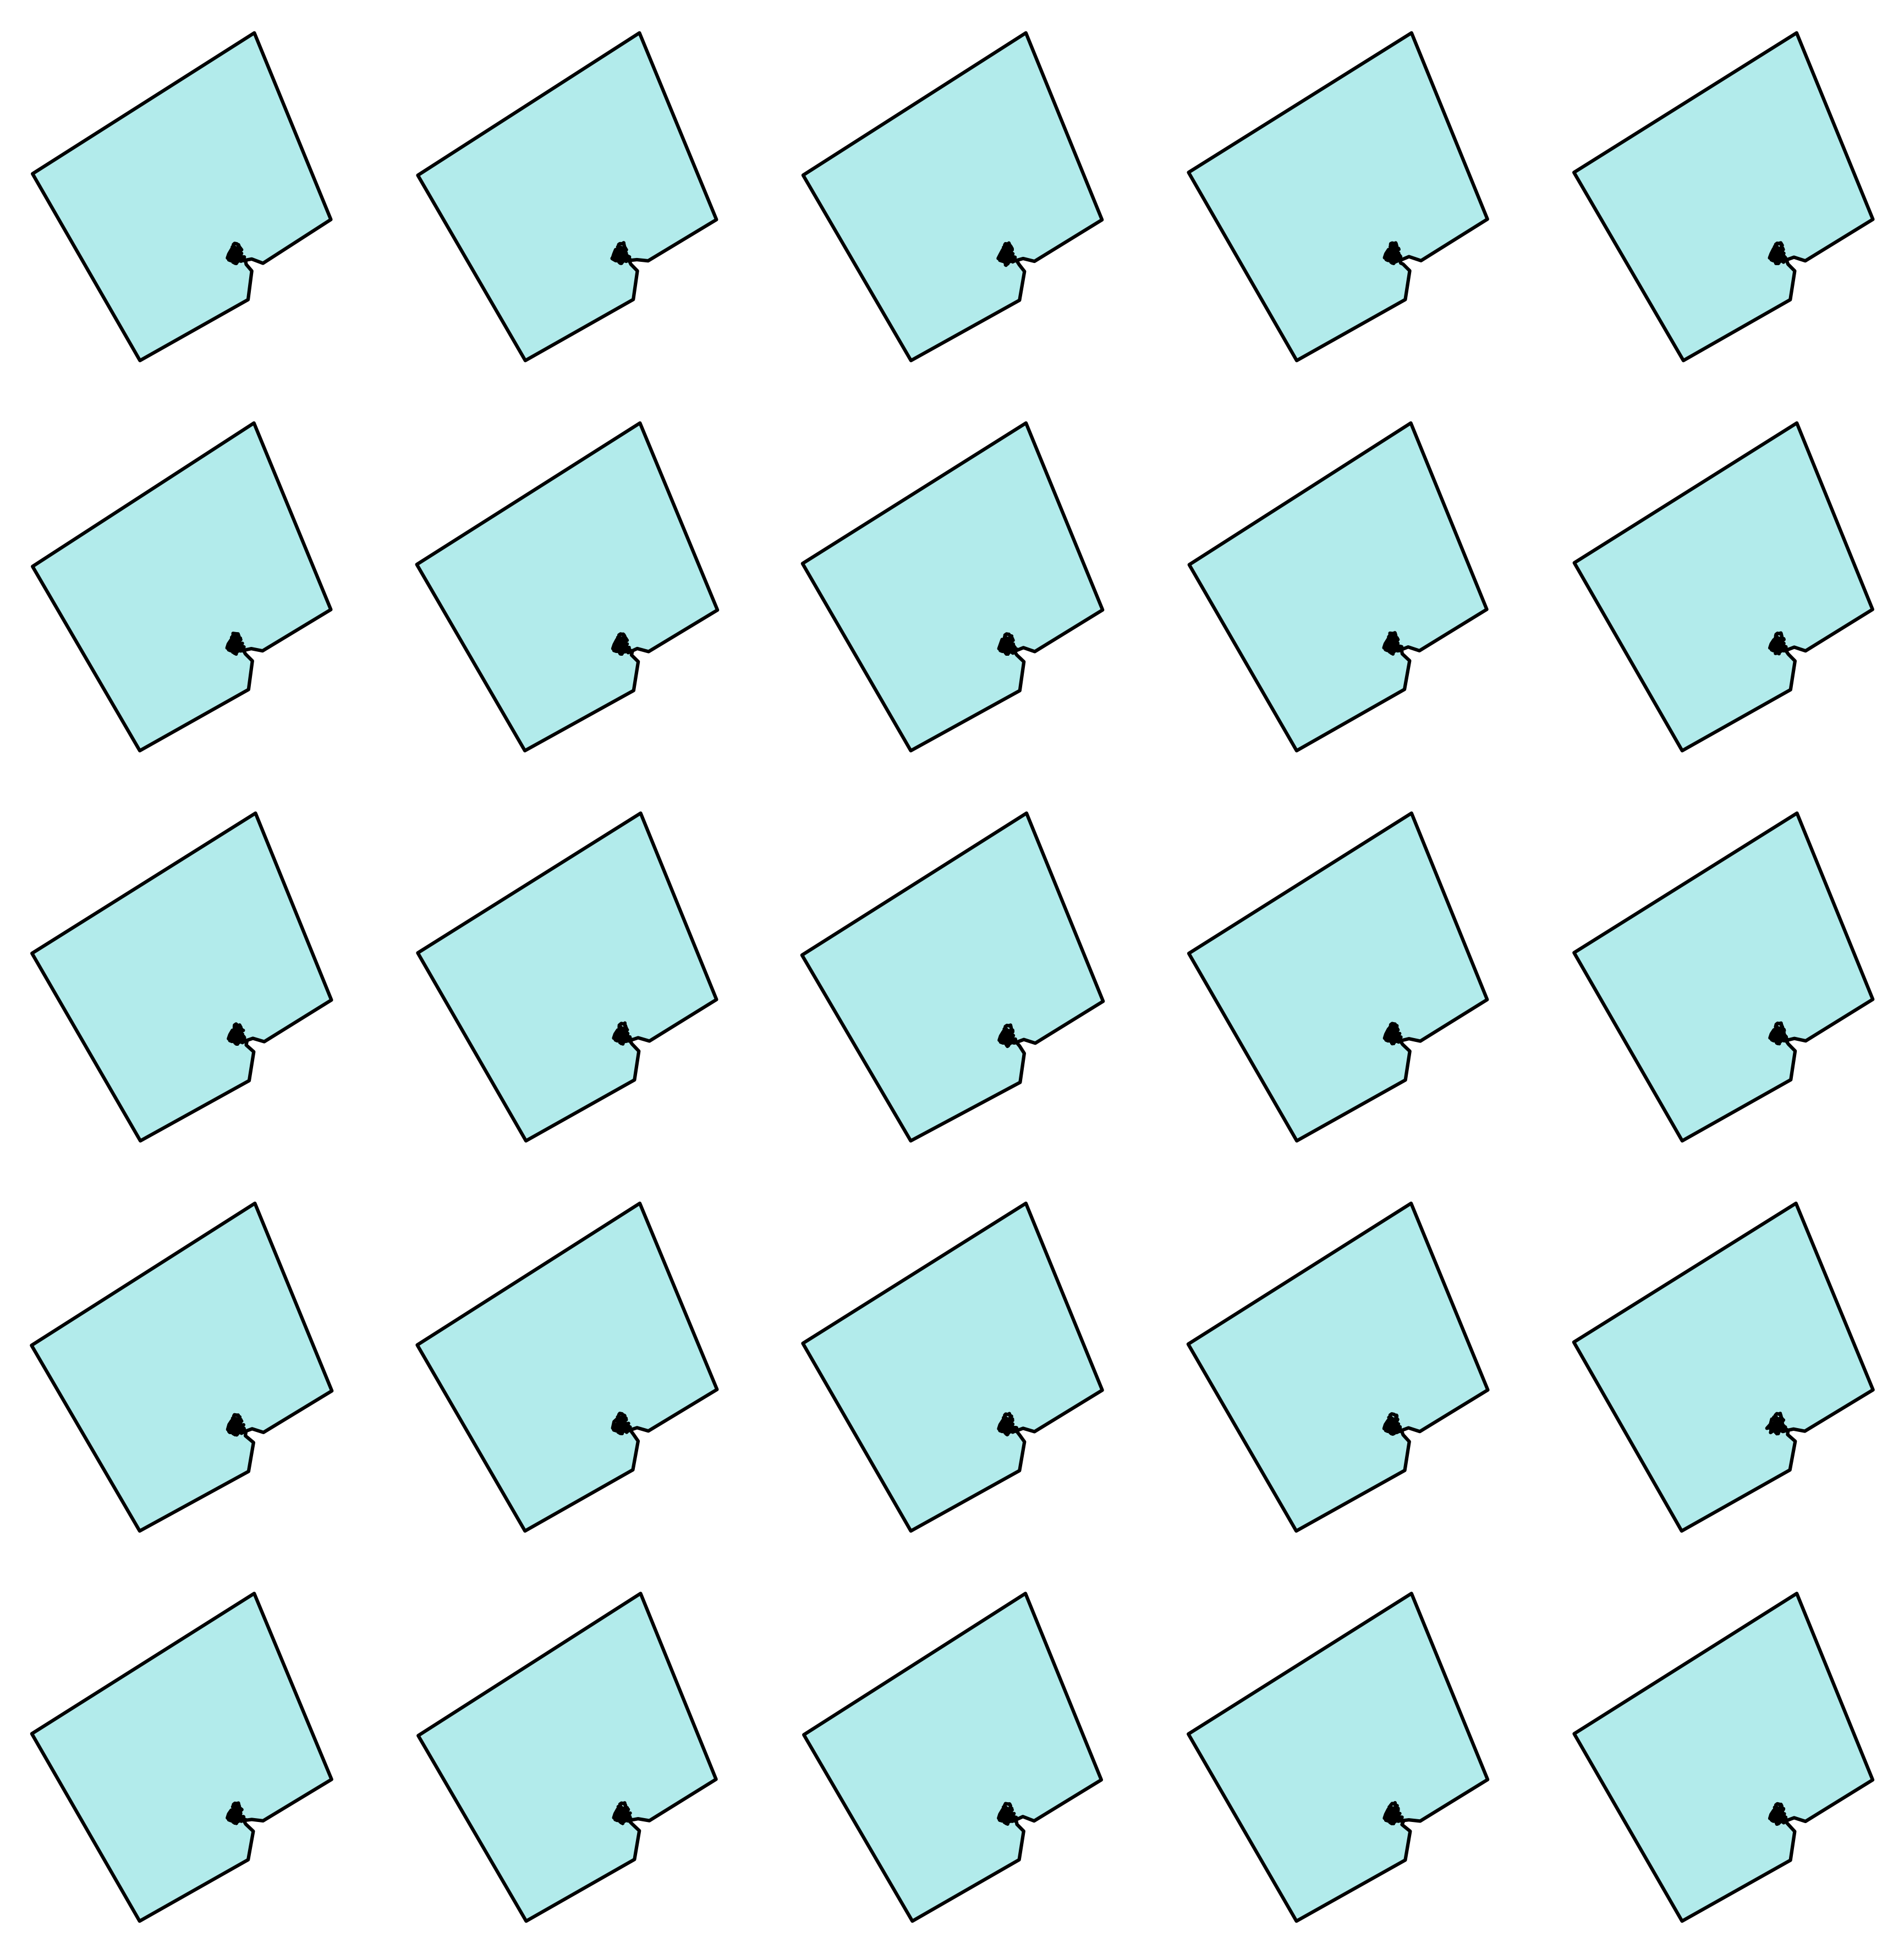
\includegraphics[width=\textwidth]{figures/GAResults/GA6/1000gens_4pars_100initpop_5pcent_mut.png}
        \caption{After 1000 generations of GA evolution.}
        \label{fig:GA6_final}
    \end{subfigure}
    \caption{GA6 starting and final population after optimising for compactness metric.}
    \label{fig:GA6_before_after_GA}
\end{figure}

\begin{figure}[H]
    \centering
    \includegraphics[width=0.75\linewidth]{figures/GAResults/GA6/fitness_curve.png}
    \caption{GA6 Genetic Algorithm Fitness Score Evolution}
    \label{fig:GA6_fitness}
\end{figure}

\subsubsection*{GA7 - Random Noise Polygon: Resolution = 200; Number of Parents = 20; Initial Population = 100}

\begin{figure}[H]
    \centering
    \begin{subfigure}[b]{0.45\textwidth}
        \centering
        \includegraphics[width=\textwidth]{figures/GAResults/GA7/200point_initial_pop.png}
        \caption{Initial starting population}
        \label{fig:GA7_starting}
    \end{subfigure}
    \hfill
    \begin{subfigure}[b]{0.45\textwidth}
        \centering
        \includegraphics[width=\textwidth]{figures/GAResults/GA7/1000gens_20pars_100initpop_5pcent_mut.png}
        \caption{After 1000 generations of GA evolution.}
        \label{fig:GA7_final}
    \end{subfigure}
    \caption{GA7 starting and final population after optimising for compactness metric.}
    \label{fig:GA7_before_after_GA}
\end{figure}

\begin{figure}[H]
    \centering
    \includegraphics[width=0.75\linewidth]{figures/GAResults/GA7/fitness_curve.png}
    \caption{GA7 Genetic Algorithm Fitness Score Evolution}
    \label{fig:GA7_fitness}
\end{figure}

\subsubsection*{GA8 - Random Noise Polygon: Resolution = 200; Number of Parents = 20; Initial Population = 1000}

\begin{figure}[H]
    \centering
    \begin{subfigure}[b]{0.45\textwidth}
        \centering
        \includegraphics[width=\textwidth]{figures/GAResults/GA8/200point_initial_pop.png}
        \caption{Initial starting population}
        \label{fig:GA8_starting}
    \end{subfigure}
    \hfill
    \begin{subfigure}[b]{0.45\textwidth}
        \centering
        \includegraphics[width=\textwidth]{figures/GAResults/GA8/1000gens_20pars_1000initpop_5pcent_mut.png}
        \caption{After 1000 generations of GA evolution.}
        \label{fig:GA8_final}
    \end{subfigure}
    \caption{GA8 starting and final population after optimising for compactness metric.}
    \label{fig:GA8_before_after_GA}
\end{figure}

\begin{figure}[H]
    \centering
    \includegraphics[width=0.75\linewidth]{figures/GAResults/GA8/fitness_curve.png}
    \caption{GA8 Genetic Algorithm Fitness Score Evolution}
    \label{fig:GA8_fitness}
\end{figure}

\subsubsection*{GA9 - Random Noise Polygon: Resolution = 300; Number of Parents = 10; Initial Population = 100}

\begin{figure}[H]
    \centering
    \begin{subfigure}[b]{0.45\textwidth}
        \centering
        \includegraphics[width=\textwidth]{figures/GAResults/GA9/300point_initial_pop.png}
        \caption{Initial starting population}
        \label{fig:GA9_starting}
    \end{subfigure}
    \hfill
    \begin{subfigure}[b]{0.45\textwidth}
        \centering
        \includegraphics[width=\textwidth]{figures/GAResults/GA9/1000gens_10pars_100initpop_5pcent_mut.png}
        \caption{After 1000 generations of GA evolution.}
        \label{fig:GA9_final}
    \end{subfigure}
    \caption{GA9 starting and final population after optimising for compactness metric.}
    \label{fig:GA9_before_after_GA}
\end{figure}

\begin{figure}[H]
    \centering
    \includegraphics[width=0.75\linewidth]{figures/GAResults/GA9/fitness_curve.png}
    \caption{GA9 Genetic Algorithm Fitness Score Evolution}
    \label{fig:GA9_fitness}
\end{figure}

% \subsubsection*{GA10 - Random Noise Polygon: Resolution = 300; Number of Parents = 10; Initial Population = 1000}

% \begin{figure}[H]
%     \centering
%     \begin{subfigure}[b]{0.45\textwidth}
%         \centering
%         \includegraphics[width=\textwidth]{figures/GAResults/GA10/300point_initial_pop.png}
%         \caption{Initial starting population}
%         \label{fig:GA10_starting}
%     \end{subfigure}
%     \hfill
%     \begin{subfigure}[b]{0.45\textwidth}
%         \centering
%         \includegraphics[width=\textwidth]{figures/GAResults/GA10/1000gens_10pars_1000initpop_5pcent_mut.png}
%         \caption{After 1000 generations of GA evolution.}
%         \label{fig:GA10_final}
%     \end{subfigure}
%     \caption{GA10 starting and final population after optimising for compactness metric.}
%     \label{fig:GA10_before_after_GA}
% \end{figure}

% \begin{figure}[H]
%     \centering
%     \includegraphics[width=0.75\linewidth]{figures/GAResults/GA10/fitness_curve.png}
%     \caption{GA10 Genetic Algorithm Fitness Score Evolution}
%     \label{fig:GA10_fitness}
% \end{figure}

\subsubsection{Genetic Algorithm - Latent Representation Results}
The following results demonstrate the evolution of the genetic algorithm for different latent dimension representations starting with 2-dimensions. For each case, we present samples from the initial starting population, as well as the generated shapes after 1000 generations when the GA is run on both the original high-design space, denoted 'original' and the latent representation 'latent'. The fitness curve is also presented to demonstrate the maximum fitness value achieved after 1000 generations in both the original and latent representation.

The initial population used in this section are obtained by sampling latent values from the latent dimensions which are then decoded by the trained VAE, generating novel designs. By using VAE generated shapes, we maintain a population that reflects realistic design points while still retaining novelty in the population due to the generative nature of the VAE. Unlike in section~\ref{random_polygon_ga}, the initial population is close to, or contain features that more closely reflect the final desired design, since the shapes are not defined by random noise, but generated by learned VAE features. As a result, the evolution of shapes is less significant in terms of visual change, and the fitness metric and is more reflective of fine-tuning to obtain an optimised fitness value. In engineering design, this may correspond to expert-driven heuristics informing the global shape, and the optimisation framework proceeds to optimise for specific features or characteristics (e.g., volume fraction, or thickness).

\subsubsection*{GA11 - 2D Latent Vector Representation: Original Resolution = 200; Number of Parents = 10; Initial Population = 50}

Figure~\ref{fig:GA11_before_after_GA} presents a sample of the initial 50 population of random shapes generated by the 2D VAE model (Model 1 in Table~\ref{tab:vae_models}). It is observed that despite being generated from the VAE trained on and realistic shape categories, the generated shapes do contain some abstract designs - though this is expected to add some variability and enable exploration amongst the population. After evolving the GA for 100 generations, the final optimised shapes, with respect to fitness, are displayed in Figure~\ref{fig:GA11__latent_final} and Figure~\ref{fig:GA11_original_final} for the latent and original design spaces respectively.

\begin{figure}[H]
    \centering
    \begin{subfigure}[b]{0.32\textwidth}
        \centering
        \includegraphics[width=\textwidth]{figures/GAResults/GA11/50_init_pop.png}
        \caption{Initial starting population}
        \label{fig:GA11_starting}
    \end{subfigure}
    \hfill
    \begin{subfigure}[b]{0.32\textwidth}
        \centering
        \includegraphics[width=\textwidth]{figures/GAResults/GA11/latent/final_generation.png}
        \caption{Latent: Final generations}
        \label{fig:GA11__latent_final}
    \end{subfigure}
    \hfill
    \begin{subfigure}[b]{0.32\textwidth}
        \centering
        \includegraphics[width=\textwidth]{figures/GAResults/GA11/original/original_final_gen.png}
        \caption{Original: Final Generation}
        \label{fig:GA11_original_final}
    \end{subfigure}
    \caption{GA11 starting and final population after optimising for compactness metric.}
    \label{fig:GA11_before_after_GA}
\end{figure}

The fitness curves are shown in Figure~\ref{fig:GA11_latent_fitness} and \ref{fig:GA11_original_fitness} shows how in the latent dimension, the GA is able to increase the maximum fitness value in the initial population from 0.07905 to 0.07925 - a marginal increase of ~0.25\% in fitness value, while when performed on the original manifold, the fitness value decreases from 0.0709 to 0.0100 after 100 generations, this is reflected in a final population of unphysical noisy shapes as shown in \ref{fig:GA11_original_final}. The maximum fitness value is achieved after less than 10 generations, though an additional marginal increase is seen at 40 generations, for the latent model in Figure~\ref{fig:GA11_latent_fitness}.

\begin{figure}[H]
    \centering
    \includegraphics[width=0.75\linewidth]{figures/GAResults/GA11/latent/100gen_fitness.png}
    \caption{GA11 - Latent: Genetic Algorithm Fitness Score Evolution}
    \label{fig:GA11_latent_fitness}
\end{figure}

\begin{figure}[H]
    \centering
    \includegraphics[width=0.75\linewidth]{figures/GAResults/GA11/original/original_200n_fitness.png}
    \caption{GA11 - Original: Genetic Algorithm Fitness Score Evolution}
    \label{fig:GA11_original_fitness}
\end{figure}

\subsubsection*{GA12 - 2D Latent Vector Representation: Resolution = 200; Number of Parents = 10; Initial Population = 10}

We also apply the GA to the same 2D latent model, but with a reduced initial population to reflect a limited size initial population due to intractable, or computationally expensive evaluations, which is typical in engineering design workflows where only final design iterations are sentenced to numerical simulation, or physical testing. 
Figure~\ref{fig:GA12_starting} shows all 10 samples in the initial population and Figure~\ref{fig:GA12_final} shows the final population after 100 generations of evolution. We see that the final shapes are not present in the initial population and demonstrate a more circular design. The fitness curve in Figure~\ref{fig:GA12_fitness} shows an increase from 0.0765 to 0.0790 fitness, again a marginal ($\lt$1.0\%) increase, though noticeable in the physical final shape. This increase in compactness is achieved after the first generation. 

\begin{figure}[H]
    \centering
    \begin{subfigure}[b]{0.45\textwidth}
        \centering
        \includegraphics[width=\textwidth]{figures/GAResults/GA12/initial_pop10.png}
        \caption{Initial starting population}
        \label{fig:GA12_starting}
    \end{subfigure}
    \hfill
    \begin{subfigure}[b]{0.45\textwidth}
        \centering
        \includegraphics[width=\textwidth]{figures/GAResults/GA12/final_pop10.png}
        \caption{After 1000 generations of GA evolution.}
        \label{fig:GA12_final}
    \end{subfigure}
    \caption{GA12 starting and final population after optimising for compactness metric.}
    \label{fig:GA12_before_after_GA}
\end{figure}

\begin{figure}[H]
    \centering
    \includegraphics[width=0.75\linewidth]{figures/GAResults/GA12/100gen_fitness.png}
    \caption{GA12 - Latent: Genetic Algorithm Fitness Score Evolution}
    \label{fig:GA12_fitness}
\end{figure}


\subsubsection*{GA13 - 3D Latent Vector Representation: Resolution = 200; Number of Parents = 10; Initial Population = 50}

Increasing the latent dimension to 3D now provides an additional gene in the genetic algorithm for which crossover and mutation can occur. The initial population is created by sampling latent values for the 3D latent dimensions for 50 samples, defining the initial population (shown in Figure~\ref{fig:GA13_starting}). After 100 generations, we observe a sample of the 50 final generation in Figure~\ref{fig:GA13_latent_final} after the GA is performed over the three latent dimensions. As previously observed, the final population samples closely reflect circular designs. Whereas when the GA is performed in the original design space, samples from the final generation are shown in Figure~\ref{fig:GA13_original_final}. The GA is observed to have agglomerated a large number of the 200 nodes to a confined region, as if getting stuck on a local minima in the GA loop, whereby the crossover and mutation is unable to perturb the points effectively to break free of this region.


\begin{figure}[H]
    \centering
    \begin{subfigure}[b]{0.32\textwidth}
        \centering
        \includegraphics[width=\textwidth]{figures/GAResults/GA13/50_init_pop.png}
        \caption{Initial starting population}
        \label{fig:GA13_starting}
    \end{subfigure}
    \hfill
    \begin{subfigure}[b]{0.32\textwidth}
        \centering
        \includegraphics[width=\textwidth]{figures/GAResults/GA13/latent/final_generation.png}
        \caption{Latent: Final Generation}
        \label{fig:GA13_latent_final}
    \end{subfigure}
    \hfill
    \begin{subfigure}[b]{0.32\textwidth}
        \centering
        \includegraphics[width=\textwidth]{figures/GAResults/GA13/original/original_final_gen.png}
        \caption{Original: Final Generation}
        \label{fig:GA13_original_final}
    \end{subfigure}
    \caption{GA13 starting and final population after optimising for compactness metric.}
    \label{fig:GA13_before_after_GA}
\end{figure}
The fitness curves in Figure~\ref{fig:GA13_latent_fitness} and \ref{fig:GA13_original_fitness} show the GAs ability to increase the fitness value from ~0.0786 to above 0.0794 in the latent space, while causing a drop to less than 0.0100 after 100 generations in the original design space. The maximum fitness value is also achieved after only 10 generations in the latent space. 

\begin{figure}[H]
    \centering
    \includegraphics[width=0.75\linewidth]{figures/GAResults/GA13/latent/100gen_fitness.png}
    \caption{GA13 Genetic Algorithm Fitness Score Evolution}
    \label{fig:GA13_latent_fitness}
\end{figure}
\begin{figure}[H]
    \centering
    \includegraphics[width=0.75\linewidth]{figures/GAResults/GA13/original/original_fitness_plot.png}
    \caption{GA13 Genetic Algorithm Fitness Score Evolution}
    \label{fig:GA13_original_fitness}
\end{figure}

\subsubsection*{GA14 - 3D Latent Vector Representation: Resolution = 200; Number of Parents = 10; Initial Population = 10}
Reducing the starting population 10 and running the GA for 100 generations reveals an increase in the maximum fitness value from ~0.0774 to 0.0780 as shown in Figure~\ref{fig:GA14_fitness}, however, the initial population used in this example is less diverse, and only one of the initial population demonstrating some features similar to a circular design. It is observed that visually, the final population of optimised shapes very closely match that of the circular like shape in the initial population, with some very minor deviations around the edge. This lack of diversity in the original population is reflected by lack of novelty or change in the final population.

\begin{figure}[H]
    \centering
    \begin{subfigure}[b]{0.45\textwidth}
        \centering
        \includegraphics[width=\textwidth]{figures/GAResults/GA14/init_pop10.png}
        \caption{Initial starting population}
        \label{fig:GA14_starting}
    \end{subfigure}
    \hfill
    \begin{subfigure}[b]{0.45\textwidth}
        \centering
        \includegraphics[width=\textwidth]{figures/GAResults/GA14/final_pop10.png}
        \caption{After 1000 generations of GA evolution.}
        \label{fig:GA14_final}
    \end{subfigure}
    \caption{GA14 starting and final population after optimising for compactness metric.}
    \label{fig:GA14_before_after_GA}
\end{figure}

\begin{figure}[H]
    \centering
    \includegraphics[width=0.75\linewidth]{figures/GAResults/GA14/100gen_fitness.png}
    \caption{GA14 Genetic Algorithm Fitness Score Evolution}
    \label{fig:GA14_fitness}
\end{figure}

\subsubsection*{GA15 - 4D Latent Vector Representation: Original Resolution = 200; Number of Parents = 10; Initial Population = 50}

A similar result is obtained when performing the GA optimisation on a 4D latent representation, where the final generation after optimisation tends towards circular designs (see Figure~\ref{fig:GA15_latent_final} and the original design space results in abstract shapes, with points fixated on a particular region (see Figure~\ref{fig:GA15_origina_final}).
Observing the fitness curve (Figure~\ref{fig:GA15_latent_final}) does however demonstrate the maximum fitness value is achieved more incrementally, with a gradual increase from ~0.0778 to ~0.0790 between generations 1 and 10, compared to the almost immediate increase seen for the 2D model and 3D latent dimensions. Similarly, when performed on the high-dimensional design space, the GA results in a significant drop in the fitness function towards 0, and then a gradual increase reaching ~0.01 fitness value after 100 generations.

\begin{figure}[H]
    \centering
    \begin{subfigure}[b]{0.32\textwidth}
        \centering
        \includegraphics[width=\textwidth]{figures/GAResults/GA15/50initial_pop.png}
        \caption{Initial starting population}
        \label{fig:GA15_starting}
    \end{subfigure}
    \hfill
    \begin{subfigure}[b]{0.32\textwidth}
        \centering
        \includegraphics[width=\textwidth]{figures/GAResults/GA15/latent/final_generation.png}
        \caption{Latent: Final Generation}
        \label{fig:GA15_latent_final}
    \end{subfigure}
    \hfill
    \begin{subfigure}[b]{0.32\textwidth}
        \centering
        \includegraphics[width=\textwidth]{figures/GAResults/GA15/original/original_final_gen.png}
        \caption{Original: Final Generation}
        \label{fig:GA15_origina_final}
    \end{subfigure}
    \caption{GA15 starting and final population after optimising for compactness metric.}
    \label{fig:GA15_before_after_GA}
\end{figure}

\begin{figure}[H]
    \centering
    \includegraphics[width=0.75\linewidth]{figures/GAResults/GA15/latent/100gens_10pars_5pcentmut.png}
    \caption{GA15 Genetic Algorithm Fitness Score Evolution (latent design space)}
    \label{fig:GA15_fitness}
\end{figure}

\begin{figure}[H]
    \centering
    \includegraphics[width=0.75\linewidth]{figures/GAResults/GA15/original/original_fitness.png}
    \caption{GA15 Genetic Algorithm Fitness Score Evolution (original design space)}
    \label{fig:GA15_fitness}
\end{figure}

\subsubsection*{GA16 - 4D Latent Vector Representation: Resolution = 200; Number of Parents = 10; Initial Population = 10}

When deploying the GA to the 4D latent representation with an initial population of 10 samples, we see after 100 generations the final generation always identically reflect mirror the circular like shape in the initial population in Figure~\ref{fig:GA16_starting}, despite the fitness curve in Figure~\ref{fig:GA16_fitness} showing an increase over the 100 generations to a maximum of ~0.07855, though with no plateau in the fitness value is observed.

\begin{figure}[H]
    \centering
    \begin{subfigure}[b]{0.45\textwidth}
        \centering
        \includegraphics[width=\textwidth]{figures/GAResults/GA16/init_pop10.png}
        \caption{Initial starting population}
        \label{fig:GA16_starting}
    \end{subfigure}
    \hfill
    \begin{subfigure}[b]{0.45\textwidth}
        \centering
        \includegraphics[width=\textwidth]{figures/GAResults/GA16/final_pop10.png}
        \caption{After 1000 generations of GA evolution.}
        \label{fig:GA16_final}
    \end{subfigure}
    \caption{GA16 starting and final population after optimising for compactness metric.}
    \label{fig:GA16_before_after_GA}
\end{figure}

\begin{figure}[H]
    \centering
    \includegraphics[width=0.75\linewidth]{figures/GAResults/GA16/100gen_fitness.png}
    \caption{GA16 Genetic Algorithm Fitness Score Evolution}
    \label{fig:GA16_fitness}
\end{figure}

\subsubsection*{GA17 - 5D Latent Vector Representation: Resolution = 200; Number of Parents = 10; Initial Population = 50}

The initial population and final populations after 100 generations are shown in Figure~\ref{fig:GA17_before_after_GA} for the latent representation and original. It is observed that the final generation after performing GA over the 5 latent dimensions results in circular like shapes, similar to what has been observed before, while the original high-dimensional shapes fail to achieve an optimal fitness value after 100 generations.

\begin{figure}[H]
    \centering
    \begin{subfigure}[b]{0.32\textwidth}
        \centering
        \includegraphics[width=\textwidth]{figures/GAResults/GA17/50_init_pop.png}
        \caption{Initial starting population}
        \label{fig:GA17_starting}
    \end{subfigure}
    \hfill
    \begin{subfigure}[b]{0.32\textwidth}
        \centering
        \includegraphics[width=\textwidth]{figures/GAResults/GA17/latent/final_generation.png}
        \caption{Latent: Final Generation}
        \label{fig:GA17_final}
    \end{subfigure}
    \hfill
    \begin{subfigure}[b]{0.32\textwidth}
        \centering
        \includegraphics[width=\textwidth]{figures/GAResults/GA17/original/original_final_gen.png}
        \caption{Original: Final Generation}
        \label{fig:GA17_final}
    \end{subfigure}
    \caption{GA17 starting and final population after optimising for compactness metric.}
    \label{fig:GA17_before_after_GA}
\end{figure}

\begin{figure}[H]
    \centering
    \includegraphics[width=0.75\linewidth]{figures/GAResults/GA17/latent/100gen_fitness.png}
    \caption{GA17 - Latent: Genetic Algorithm Fitness Score Evolution}
    \label{fig:GA17_latent_fitness}
\end{figure}
\begin{figure}[H]
    \centering
    \includegraphics[width=0.75\linewidth]{figures/GAResults/GA17/original/original_fitness.png}
    \caption{GA17 - Original: Genetic Algorithm Fitness Score Evolution}
    \label{fig:GA17_original_fitness}
\end{figure}

\subsubsection*{GA18 - 5D Latent Vector Representation: Resolution = 200; Number of Parents = 10; Initial Population = 10}

\begin{figure}[H]
    \centering
    \begin{subfigure}[b]{0.45\textwidth}
        \centering
        \includegraphics[width=\textwidth]{figures/GAResults/GA18/init_pop10.png}
        \caption{Initial starting population}
        \label{fig:GA18_starting}
    \end{subfigure}
    \hfill
    \begin{subfigure}[b]{0.45\textwidth}
        \centering
        \includegraphics[width=\textwidth]{figures/GAResults/GA18/final_pop10.png}
        \caption{After 1000 generations of GA evolution.}
        \label{fig:GA18_final}
    \end{subfigure}
    \caption{GA18 starting and final population after optimising for compactness metric.}
    \label{fig:GA18_before_after_GA}
\end{figure}

\begin{figure}[H]
    \centering
    \includegraphics[width=0.75\linewidth]{figures/GAResults/GA18/10gen_fitness.png}
    \caption{GA18 Genetic Algorithm Fitness Score Evolution}
    \label{fig:GA18_fitness}
\end{figure}

\subsubsection*{GA19 - 6D Latent Vector Representation: Resolution = 200; Number of Parents = 10; Initial Population = 50}

\begin{figure}[H]
    \centering
    \begin{subfigure}[b]{0.32\textwidth}
        \centering
        \includegraphics[width=\textwidth]{figures/GAResults/GA19/50init_pop.png}
        \caption{Initial starting population}
        \label{fig:GA19_starting}
    \end{subfigure}
    \hfill
    \begin{subfigure}[b]{0.32\textwidth}
        \centering
        \includegraphics[width=\textwidth]{figures/GAResults/GA19/latent/final_generation.png}
        \caption{After 1000 generations of GA evolution.}
        \label{fig:GA19_latent_final}
    \end{subfigure}
    \hfill
    \begin{subfigure}[b]{0.32\textwidth}
        \centering
        \includegraphics[width=\textwidth]{figures/GAResults/GA19/original/original_final_gen.png}
        \caption{Original: Final Generation}
        \label{fig:GA19_original_final}
    \end{subfigure}
    \caption{GA19 starting and final population after optimising for compactness metric.}
    \label{fig:GA19_before_after_GA}
\end{figure}

\begin{figure}[H]
    \centering
    \includegraphics[width=0.75\linewidth]{figures/GAResults/GA19/latent/100gen_fitness.png}
    \caption{GA19 Genetic Algorithm Fitness Score Evolution}
    \label{fig:GA19_fitness}
\end{figure}

\subsubsection*{GA20 - 6D Latent Vector Representation: Resolution = 200; Number of Parents = 10; Initial Population = 10}

\begin{figure}[H]
    \centering
    \begin{subfigure}[b]{0.45\textwidth}
        \centering
        \includegraphics[width=\textwidth]{figures/GAResults/GA20/init_pop10.png}
        \caption{Initial starting population}
        \label{fig:GA19_starting}
    \end{subfigure}
    \hfill
    \begin{subfigure}[b]{0.45\textwidth}
        \centering
        \includegraphics[width=\textwidth]{figures/GAResults/GA20/final_pop10.png}
        \caption{After 1000 generations of GA evolution.}
        \label{fig:GA20_final}
    \end{subfigure}
    \caption{GA20 starting and final population after optimising for compactness metric.}
    \label{fig:GA20_before_after_GA}
\end{figure}

\begin{figure}[H]
    \centering
    \includegraphics[width=0.75\linewidth]{figures/GAResults/GA20/10gen_fitness.png}
    \caption{GA20 Genetic Algorithm Fitness Score Evolution}
    \label{fig:GA20_fitness}
\end{figure}




\newpage{}

\section{Conclusion}

\newpage{}
\section{Appendix}











\newpage{}
\bibliographystyle{agsm}
\bibliography{sample}

\end{document}